\documentclass[12pt,xcolor=table,aspectratio=169]{beamer}
\usetheme{Frankfurt}
\usecolortheme{rose}
\usepackage{amsthm}
\usepackage{amsmath}
\usepackage{bbm}
\usepackage{amsfonts}
\usepackage{amssymb}
\usepackage{graphicx}
\usepackage{hyperref}
\usepackage[flushleft]{threeparttable}
\usepackage{tabularx}
\usepackage{booktabs}
\usepackage{siunitx}
\usepackage{tikz}
\usetikzlibrary{decorations.pathreplacing,angles,quotes}
%\usepackage{enumitem}% http://ctan.org/pkg/enumitem

%set up course and number

\newcommand{\ClassName}{TBD}
\newcommand{\ClassNumber}{TBD}
\newcommand{\Topic}{TBD}

% Some optional colors. Change or add as you see fit.
%---------------------------------------------------
 \definecolor{ualbertagreen}{HTML}{007C41}
\definecolor{ualbertagold}{HTML}{FFDB05}

\definecolor{calloutgrey}{HTML}{D9D9D9}


%set fonts
\setbeamerfont{subtitle}{size=\large,shape=\scshape,series=\bfseries}
\setbeamerfont{title}{size=\Large,shape=\scshape,series=\bfseries}
\setbeamerfont{author}{size=\large}
\setbeamerfont{date}{size=\large}
\setbeamerfont{caption}{size=\scriptsize}


% Some optional color adjustments to Beamer. Change as you see fit.
%------------------------------------------------------------------
\setbeamercolor{frametitle}{fg=ualbertagreen,bg=white}
\setbeamercolor{title}{fg=ualbertagreen,bg=white}
\setbeamercolor{author}{fg=ualbertagreen,bg=white}
\setbeamercolor{date}{fg=ualbertagreen,bg=white}
\setbeamercolor{local structure}{fg=ualbertagreen}
\setbeamercolor{section in toc}{fg=ualbertagreen,bg=white}
% \setbeamercolor{subsection in toc}{fg=ualbertagreen,bg=white}
\setbeamercolor{footline}{fg=ualbertagreen!50, bg=white}

% definition boxes
\setbeamercolor{block title}{bg=ualbertagreen,fg=white}
\setbeamercolor{block body}{parent=normal text,use=block title,bg=calloutgrey}
%\setbeamercolor{block body}{parent=normal text,use=block title,bg=block title.bg!30!bg}


\setbeamercolor{upper separation line head}{bg=ualbertagreen}
\setbeamercolor{lower separation line head}{bg=ualbertagold}
\setbeamercolor{middle separation line head}{bg=ualbertagold}
\setbeamercolor{frametitle}{fg=ualbertagreen,bg=white}



\setbeamercolor{section in head/foot}{bg=white,fg=ualbertagreen}
\setbeamercolor{author in head/foot}{bg=white,fg=ualbertagreen}
\setbeamercolor{date in head/foot}{bg=white,,fg=ualbertagreen}
\setbeamercolor{title in head/foot}{bg=white,fg=ualbertagreen}

\setbeamercolor{headline}{bg=white,fg=ualbertagreen}




\setbeamercolor*{middle separation line head}{bg=ualbertagreen}
\setbeamercolor*{alerted text}{fg=ualbertagreen}
\setbeamercolor*{example text}{fg=black}
\setbeamercolor*{structure}{fg=black}


\let\Tiny=\tiny



\logo{
   %\ifnum\insertpagenumber>1
   \tikz [remember picture,overlay]
    \node[yshift=.3cm,xshift=1.5cm] at (current page.south west)
        %or: (current page.center)
        {
\includegraphics[width=1in]{../images/UA-ASB-COLOUR.png}};
    %\fi
%
\includegraphics[height=0.8cm]{../images/UA-ASB-COLOUR.png}\vspace{220pt}
}


\setbeamertemplate{title page}{%
  \vbox{}
    \vspace{.5cm}% NEW
  \begingroup
    \centering
    \begin{beamercolorbox}[sep=8pt,center]{title}
      \usebeamerfont{title}\ClassNumber: \ClassName\par%
      \usebeamerfont{title}\inserttitle\par%
     \ifx\insertsubtitle\@empty%
      \else%
        \vskip0.05em%
        {\usebeamerfont{subtitle}\usebeamercolor[fg]{subtitle}\insertsubtitle\par}%
      \fi%
    \end{beamercolorbox}%
    \begin{beamercolorbox}[sep=8pt,center]{author}
      \usebeamerfont{author}\insertauthor
    \end{beamercolorbox}
    \begin{beamercolorbox}[sep=8pt,center]{institute}
      \usebeamerfont{institute}\insertinstitute
    \end{beamercolorbox}

    %\vspace{0.5cm}% NEW
    %\begin{beamercolorbox}[sep=8pt,center]{date}
    %  \usebeamerfont{date}\insertdate
    %\end{beamercolorbox}\vskip0.05em

      \endgroup
  %\vfill
}



\setbeamertemplate{frametitle}{%
    \insertframetitle\par\vskip-10pt
}



\renewcommand{\ClassName}{Business Economics, Organization and Management}
\renewcommand{\ClassNumber}{BUEC 311}

\setbeamertemplate{headline}{%
\leavevmode%
 \hbox{%
    \begin{beamercolorbox}[wd=\paperwidth,ht=5ex,dp=0ex]{white}%
    \usebeamerfont{headline}\hskip6pt\ClassNumber: \inserttitle\par%
    \insertsectionnavigationhorizontal{\paperwidth}{}{\hskip0pt plus1filll}
    \end{beamercolorbox}%
  }
}

\defbeamertemplate*{footline}{my footline}{%
    \ifnum\insertpagenumber=1
        \Tiny{%
            \hfill%
		\vspace*{1pt}%
            %\insertframenumber/\inserttotalframenumber \hspace*{0.1cm}%
            \newline%
            \color{ualbertagold}{\rule{\paperwidth}{0.4mm}}\newline%
            \color{ualbertagold}{\rule{\paperwidth}{.4mm}}%
        }
  \else%
        \Tiny{%
            \hspace{.66\paperwidth}
            %\vspace{25pt}
            \insertframenumber/\inserttotalframenumber
            \newline%
            \color{ualbertagold}{\rule{\paperwidth}{0.4mm}}\newline%
            \color{ualbertagold}{\rule{\paperwidth}{.4mm}}%
        }%
    \fi%
}


\newenvironment{itemize*}%
  {\begin{itemize}%
    \setlength{\itemsep}{0pt}%
    \setlength{\parskip}{0pt}}%
  {\end{itemize}}




\title{Supply and Demand - The Basics}


\date{BUEC 311}

\begin{document}
\setcounter{subsection}{1}
\begin{frame}
   %\tikz [remember picture,overlay]
    %\node[yshift=-1.05cm,xshift=0cm] at (current page.north)
        %or: (current page.center)
        %\node[yshift=-0.95cm,xshift=3.5cm] at (current page.north west)
        %{
\includegraphics[width=3in]{UA-ASB-COLOUR.png}};
    %    {
\includegraphics[width=.4\paperwidth]{../images/UA-ASB-COLOUR.png}}; \vspace{1cm}
   \titlepage
   \vfill
\end{frame}

\section{Introduction}

\frame{
	\frametitle{Outline}
	\begin{enumerate}
	\item The Supply-and-Demand Model
		\begin{itemize}
		\item Demand
		\item Supply
		\item Market Equilibrium
		\end{itemize}
	\item Using the Model
		\begin{itemize}
		\item Changing fundamentals.
		\item The effects of government intervention.
		\end{itemize}
	\item Applying the model in practice.
		\begin{itemize}
		\item When it works.
		\item When if fails.
		\end{itemize}
	\end{enumerate}
\vfill
}


\frame{
	\frametitle{Outline}
	\begin{enumerate}
	\item \alert{The Supply-and-Demand Model}
		\begin{itemize}
		\item Demand
		\item Supply
		\item Market Equilibrium
		\end{itemize}
	\item Using the Model
		\begin{itemize}
		\item Changing fundamentals.
		\item The effects of government intervention.
		\end{itemize}
	\item Applying the model in practice.
		\begin{itemize}
		\item When it works.
		\item When if fails.
		\end{itemize}
	\end{enumerate}
\vfill
}

\section{Demand}


\frame{
	\frametitle{Demand}
	\begin{itemize}
	\item Supply and demand is the core of almost every economic model
	\item[]
	\item This simple model is useful for understanding many markets.
		\begin{itemize}
		\item It works particularly well in markets with many buyers and sellers.
		\end{itemize}
	\item[]
	\item Why is it useful?
		\begin{itemize}
		\item We can use it to make clear predictions about how changes in fundamentals affect
market outcomes.
        \item The limitations are easy to understand
		\end{itemize}
	\end{itemize}
}

\frame{
	\frametitle{Demand}
	\begin{itemize}
	\item The first piece of the model: \textbf{Demand}
	\item[]
	\item Demand is consumer's \textit{desire} to purchase goods and services.
	\item[]
	\item What factors affect this desire? How?
	\end{itemize}
}

\frame{
	\frametitle{Demand}
	\begin{itemize}
	\item While many factors can affect consumer's desire to purchase goods and services, economists
primarily focus on how a good's \textit{own price} affects the quantity demanded.
	\end{itemize}
	\bigskip
		\begin{definition}[Quantity Demanded]
		The quantity demanded is the amount of a good or service a consumer is \textit{willing} to buy
at a given price, holding other factors constant.
		\end{definition}	
}

\frame{
	\frametitle{Demand}
	\begin{itemize}
	\item Empirical evidence suggests that the quantity demanded by consumers follows the \textit{Law
of Demand}.
	\end{itemize}
	
		\begin{definition}[Law of Demand]
		Consumers demand a higher quantity of a good or service when the price is lower (and a lower
quantity of when the price is higher), \textit{holding all other factors that influence the amount
consumers want to consume constant}.
		\end{definition}
		
	\begin{itemize}
	\item We can illustrate this relationship graphically using a \textit{demand curve}.
		\begin{itemize}
		\item To do so, let's use the example of gasoline demand.
		\end{itemize}
	\end{itemize}
}

\frame{
	\frametitle{The Demand Curve}
	%	The demand for gasoline:
	
	\begin{figure}[t!]
	\center
	\resizebox{!}{.45\linewidth}{
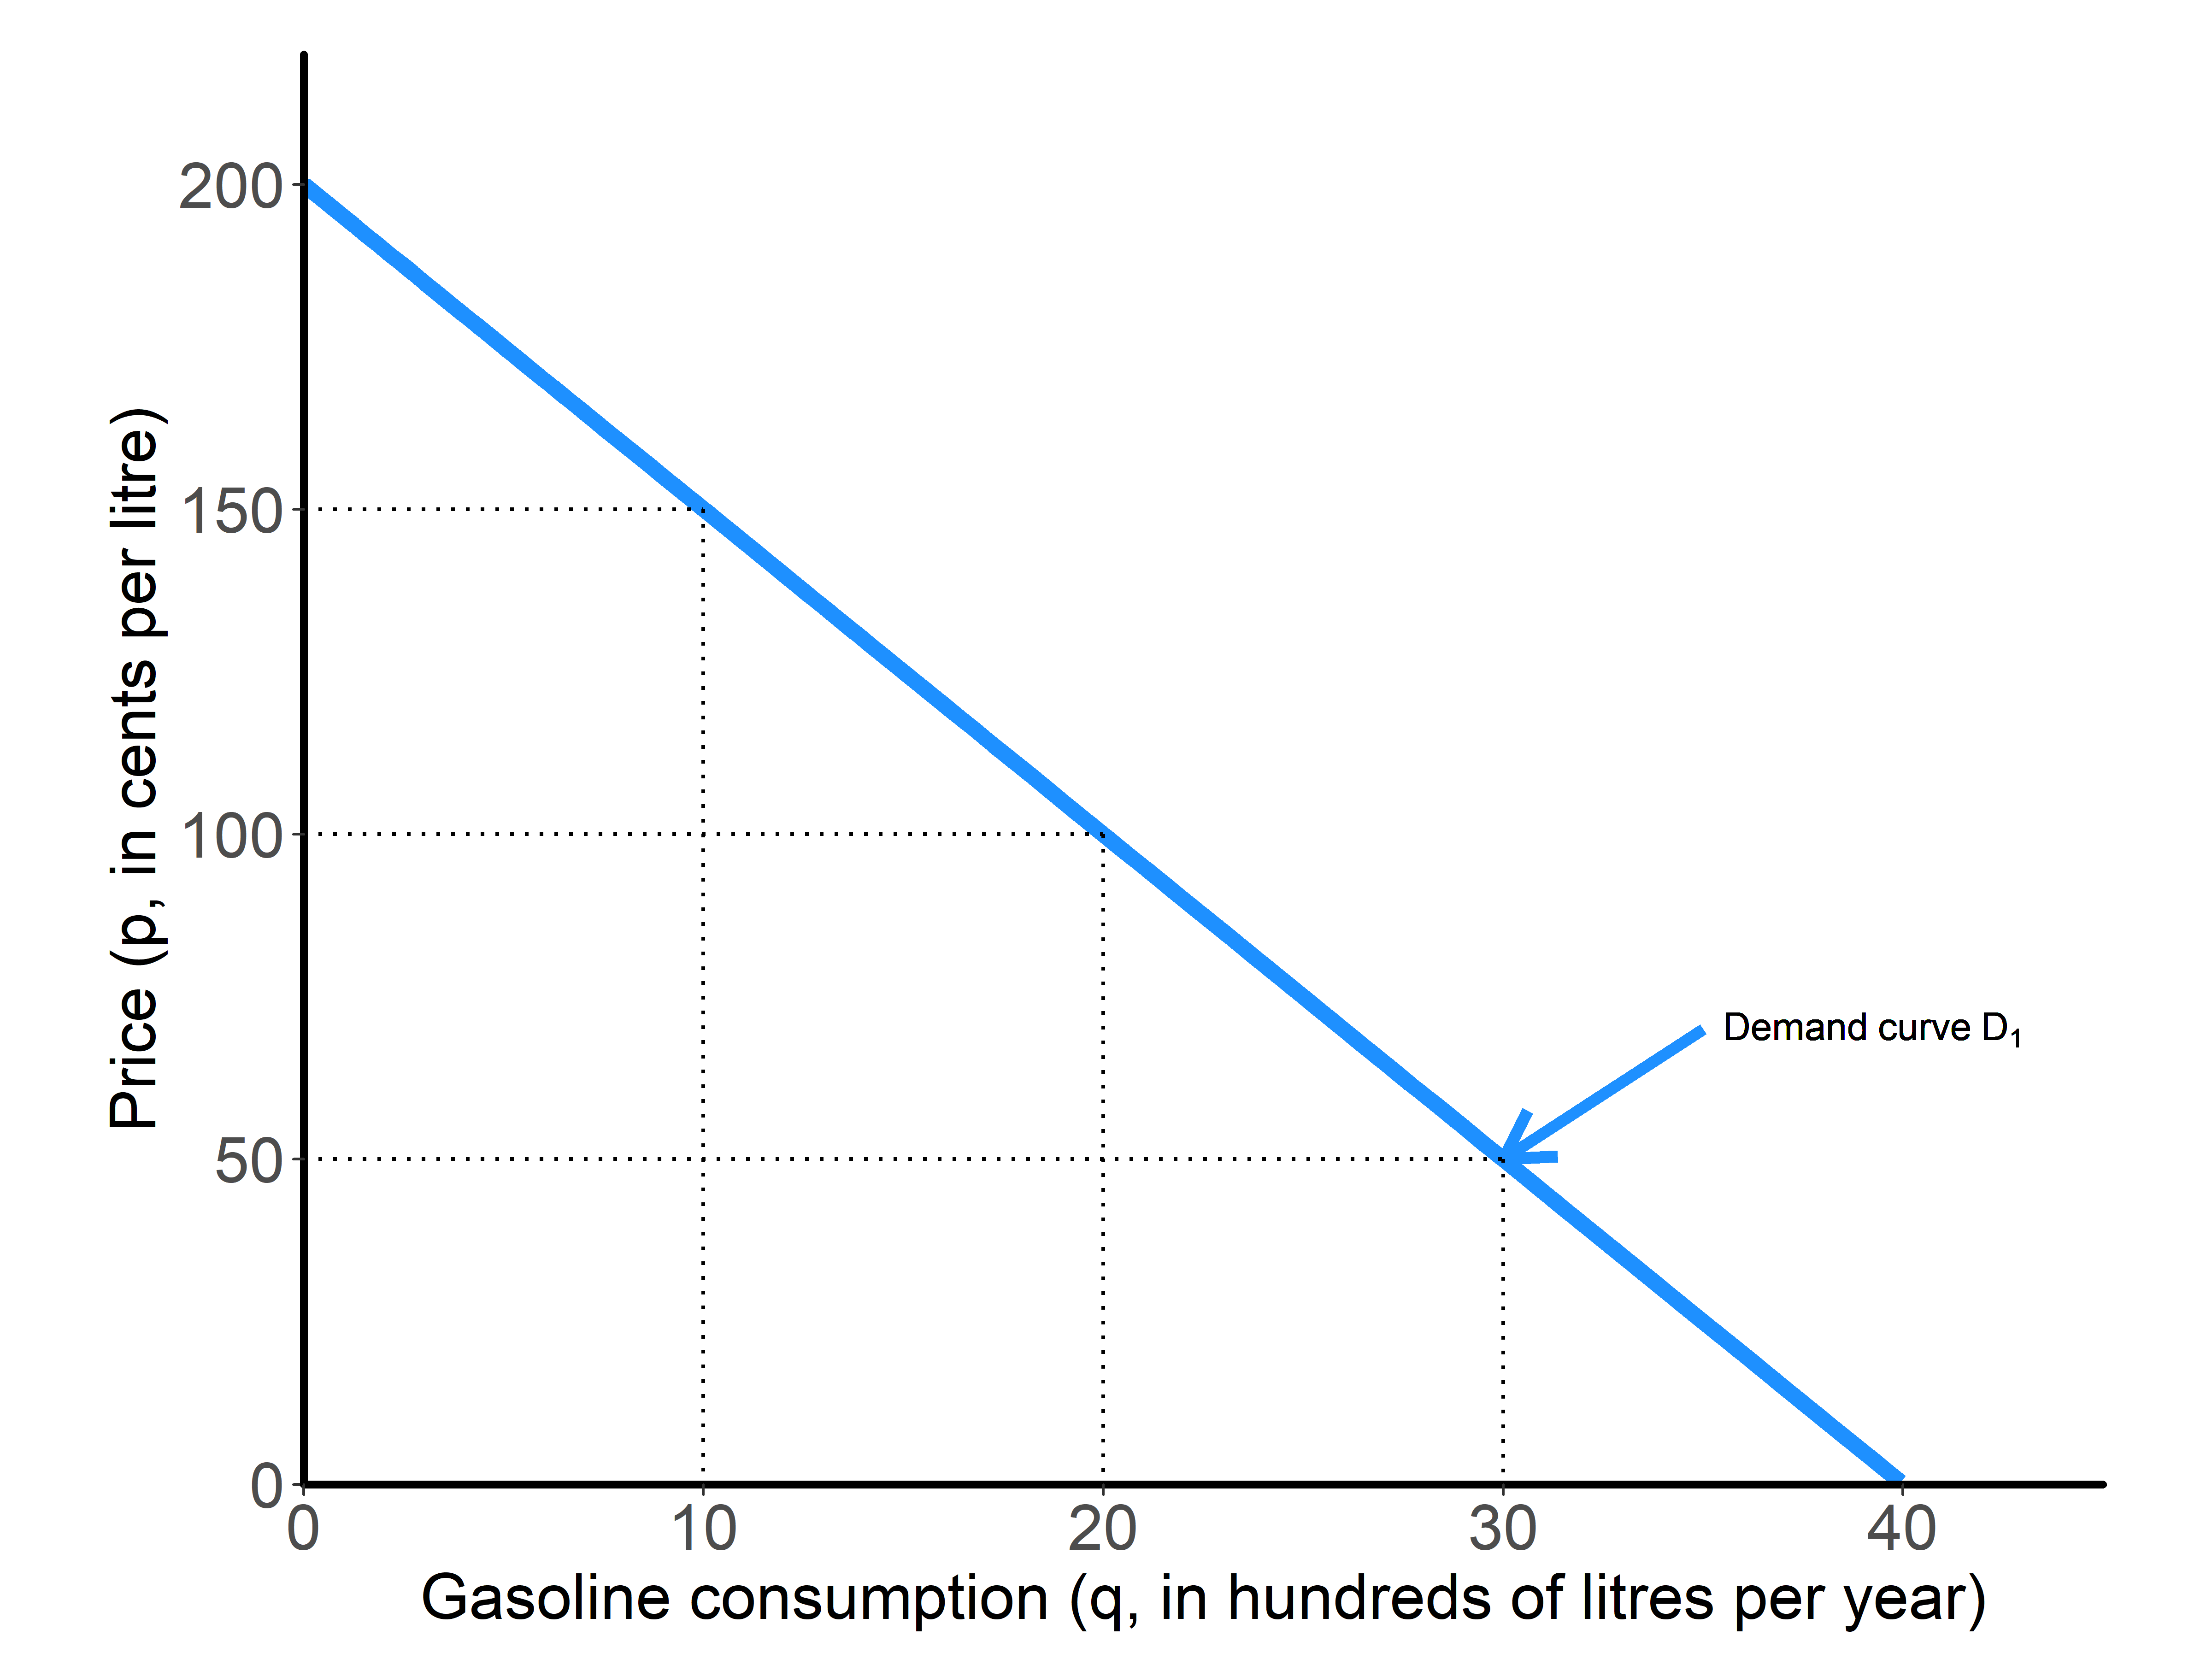
\includegraphics[width=\textwidth]{../images/gas_demand.png}
}
\caption{The demand for gasoline}
\end{figure}
}


\frame{
	\frametitle{The Demand Curve}
	%	The demand for gasoline:
	
	\begin{figure}[t!]
	\center
	\resizebox{!}{.45\linewidth}{
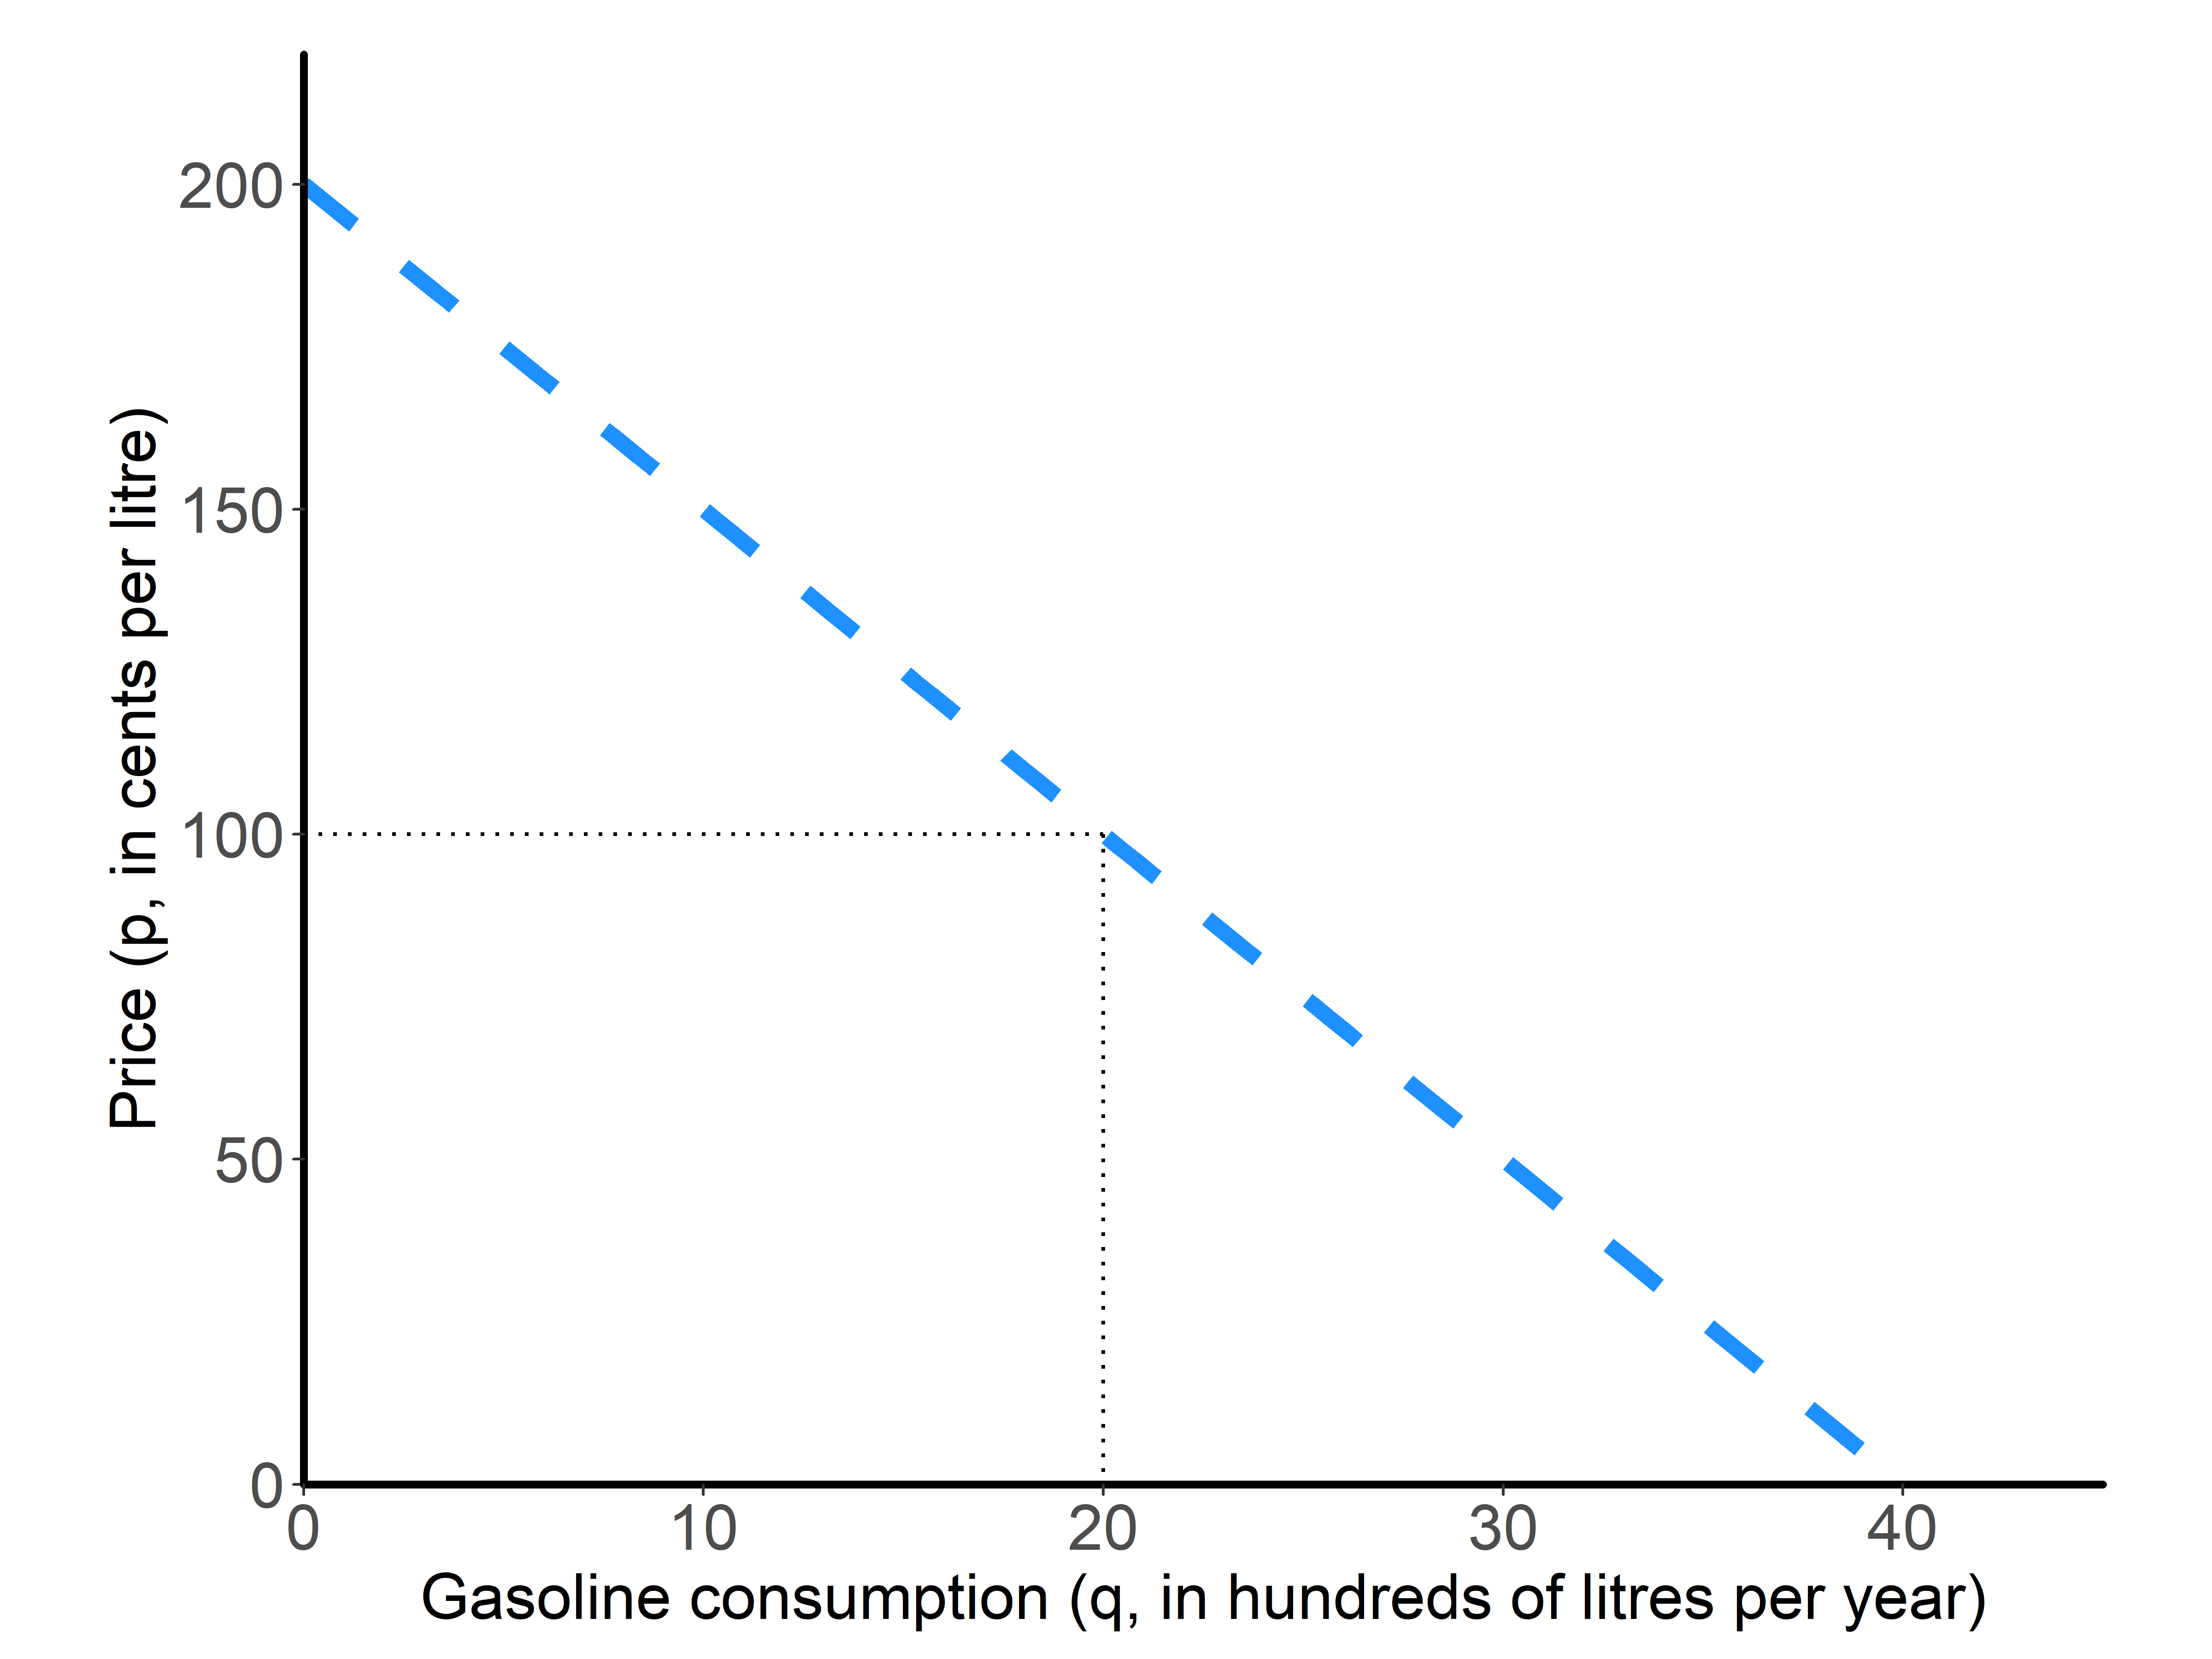
\includegraphics[width=\textwidth]{../images/gas_demand_zoom.png}
}
\caption{The demand for gasoline}
\end{figure}
}


\frame{
	\frametitle{The Demand Curve}
	\begin{itemize}
	\item The demand curve provides a concise answer to the question of what happens to the quantity
demanded as price changes, holding all other factors constant.
		\begin{itemize}
		\item Here: what happens to the demand for gasoline as the price of gasoline increases or
decreases.
		\end{itemize}
	\item[]
	\item Changes in the quantity demanded in response to a price change are referred to as
\textit{movements along the demand curve}.
	\item[]
	\item Why is the demand curve downward sloping?
	\end{itemize}
}

\frame{
	\frametitle{The Demand Curve}
	\begin{itemize}
	\item The demand curve tells us how a change in the price of a good or service affects the
quantity demanded.
		\begin{itemize}
		\item Change in $p$ $\implies$ \textit{movement along the demand curve}.
		\end{itemize}
	\item[]
	\item Recall that other factors also affect the quantity demanded.
		\begin{itemize}
		\item Change in these factors $\implies$ \textit{shift of the demand curve}.
		\end{itemize}
	\item[]
	\item As an example, let's consider an increase in household income. How would you expect that to change gasoline demand?
	\end{itemize}
}

\frame{
	\frametitle{The Demand Curve}
		%	The demand for gasoline:
	
	\begin{figure}[t!]
	\center
	\resizebox{!}{.45\linewidth}{
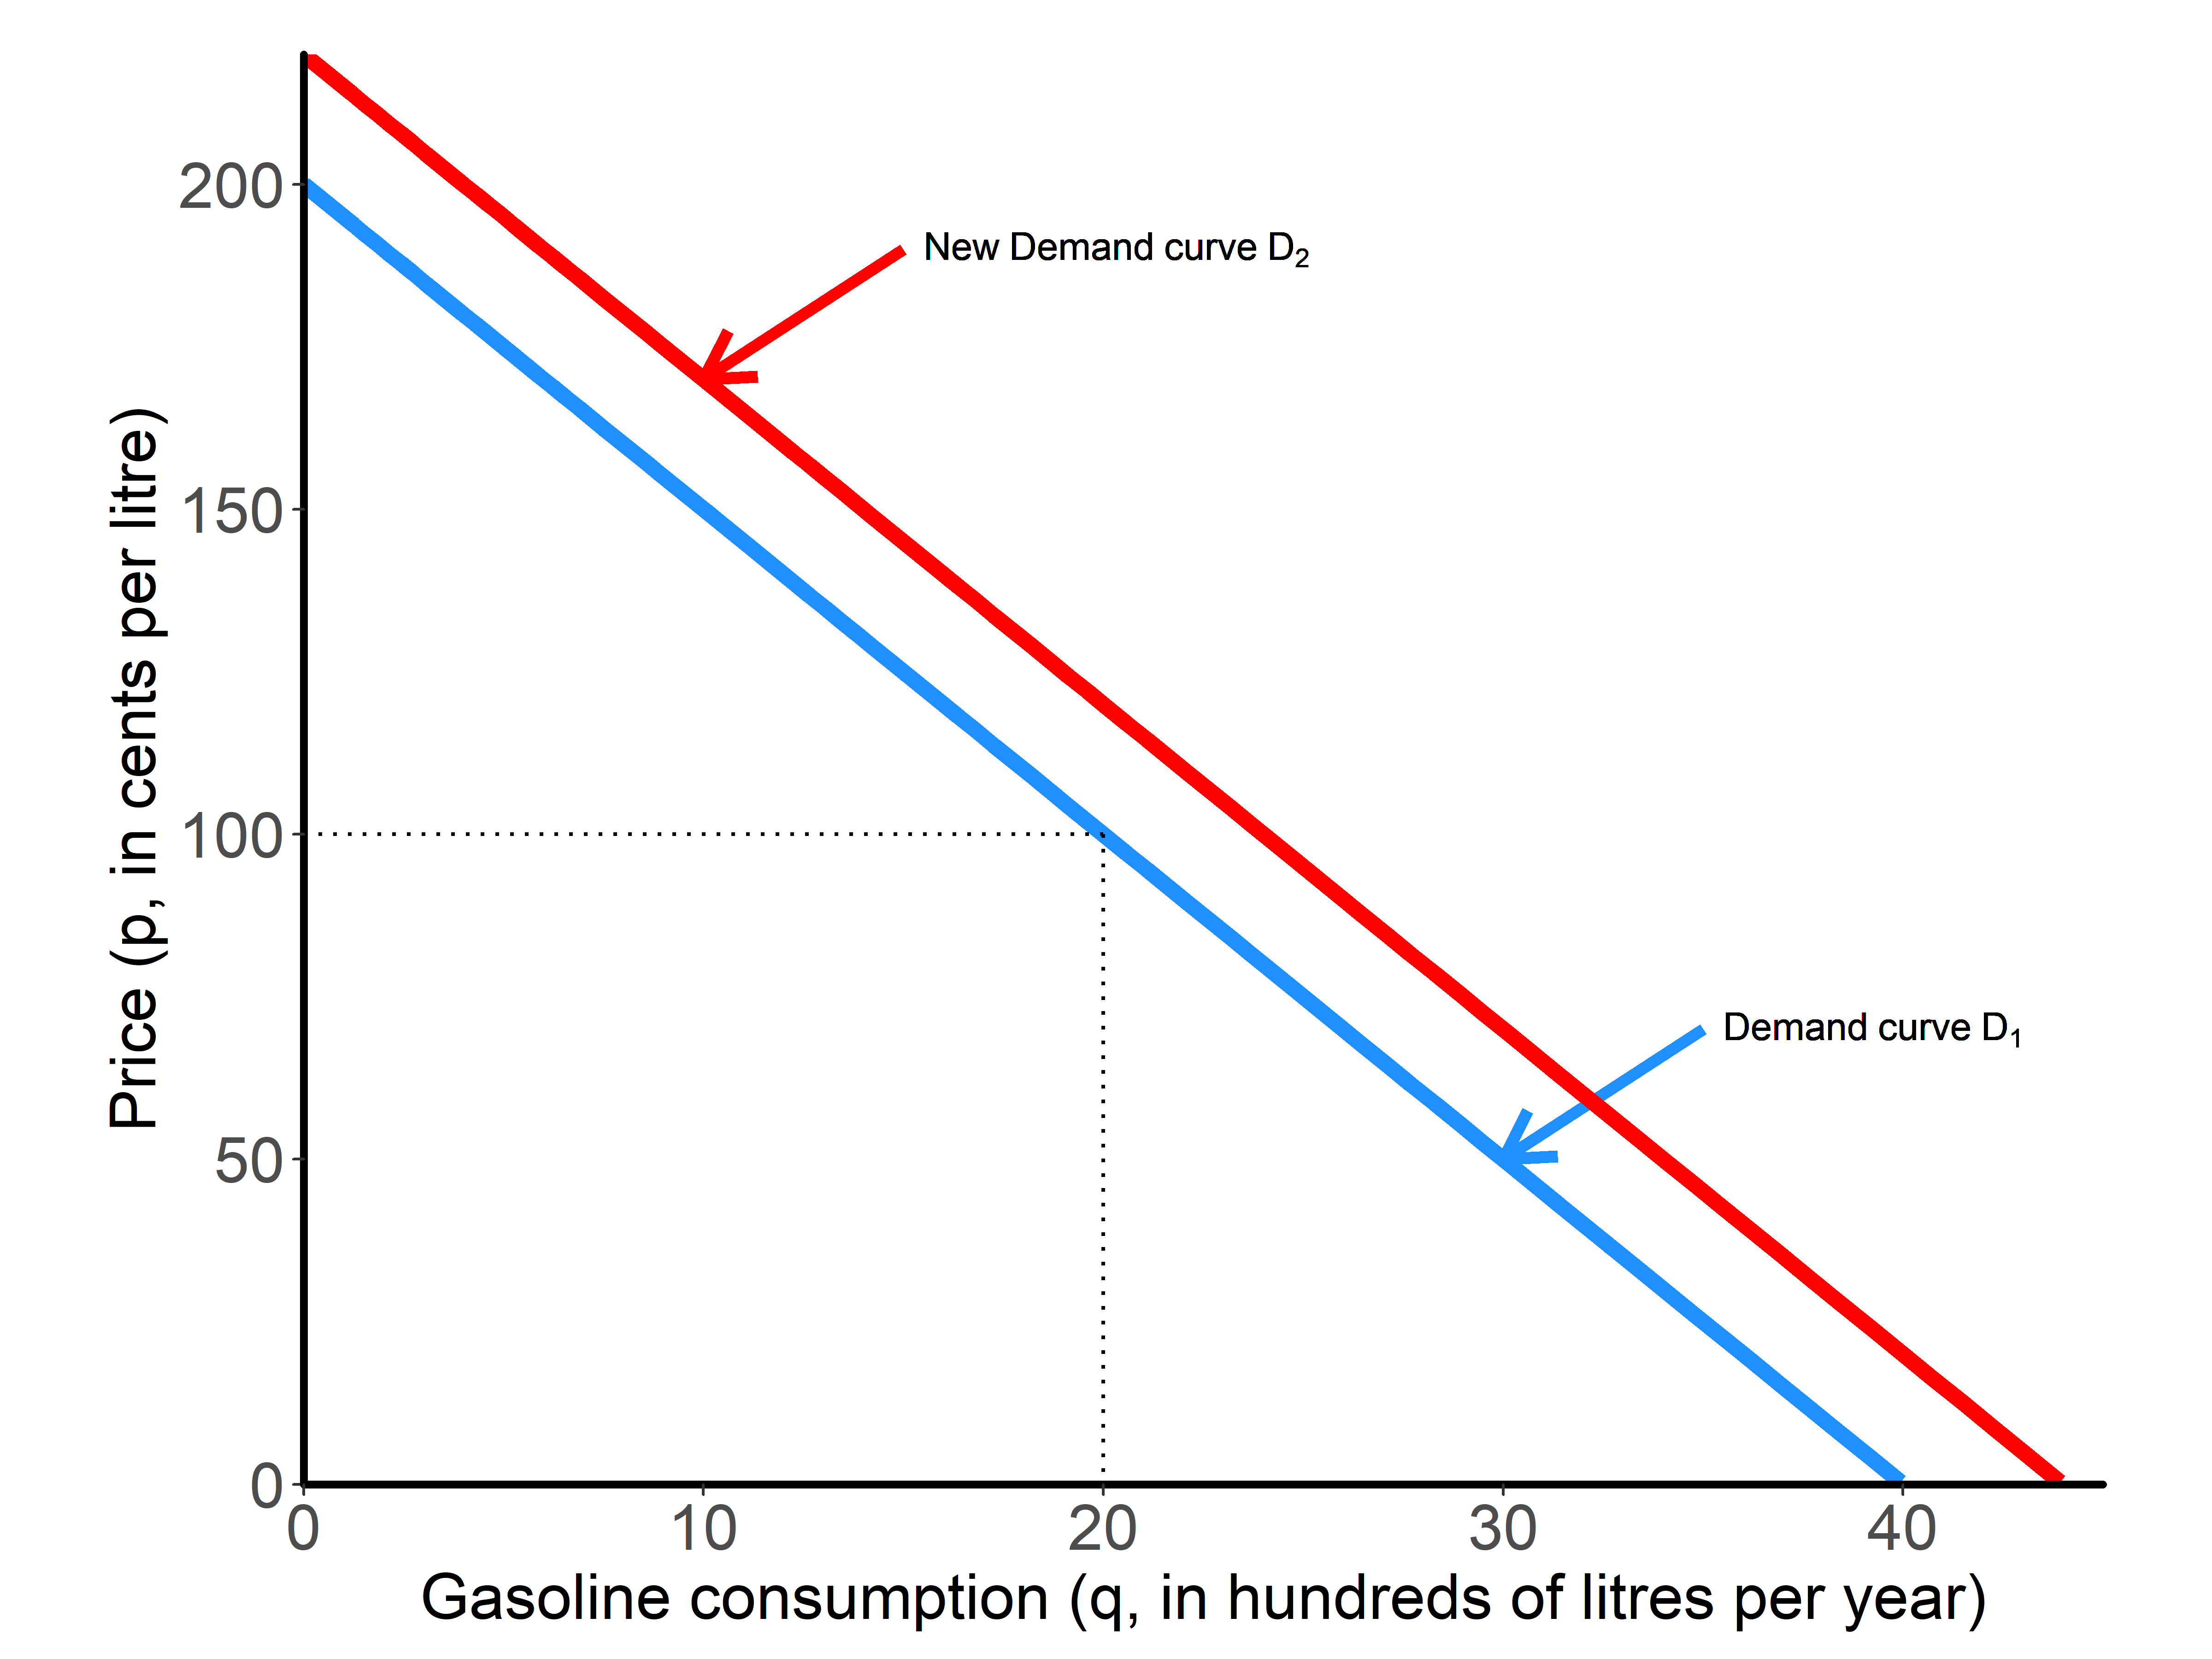
\includegraphics[width=\textwidth]{../images/gas_inc.png}
}
\caption{The effects of an income increase on the demand for gasoline}
\end{figure}
}

\frame{
	\frametitle{The Demand Curve}
		%	The demand for gasoline:
	
	\begin{figure}[t!]
	\center
	\resizebox{!}{.45\linewidth}{
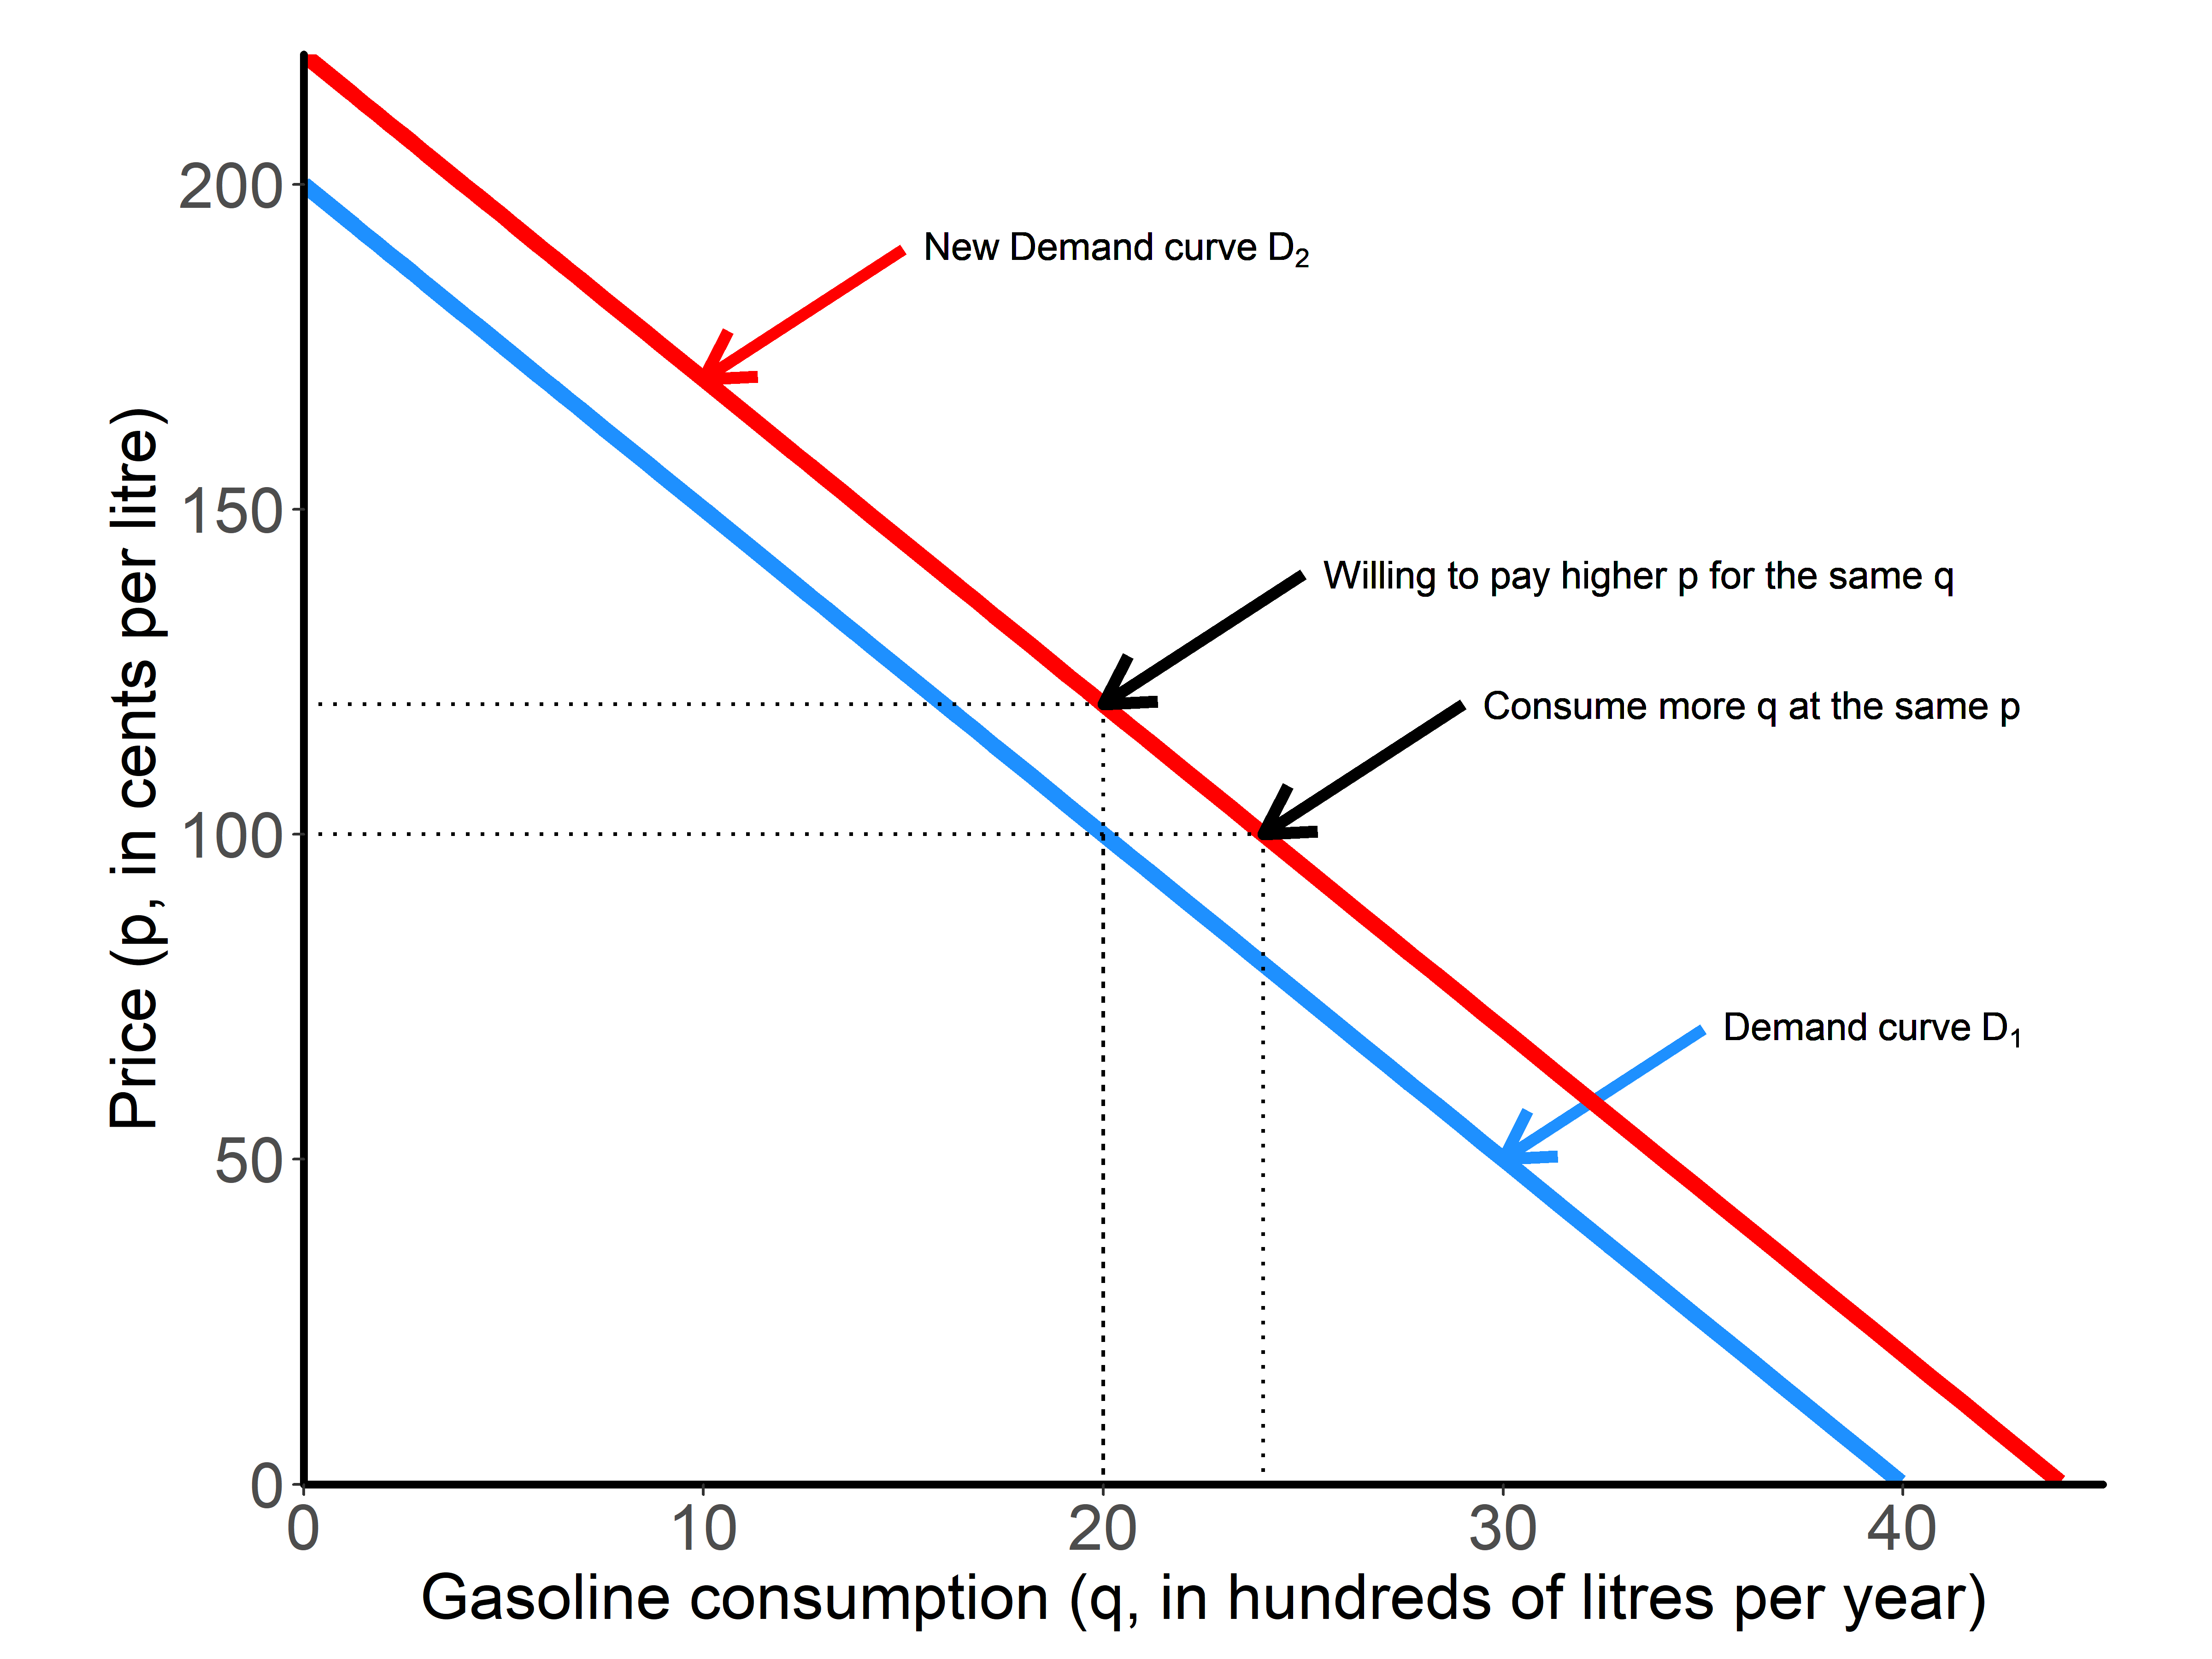
\includegraphics[width=\textwidth]{../images/gas_inc2.png}
}
\caption{The effects of an income increase on the demand for gasoline}
\end{figure}
}


\frame{
	\frametitle{The Demand Curve}
	\begin{itemize}
	\item How the demand curve shifts depends on the factor being considered.
		\begin{itemize}
		\item Income
		\item Price of substitute or compliment
		\item Tastes
		\item Government rules/regulations
		\end{itemize}
	\item[]
	\item As another example, let's consider the effects of an increase in the price tolls in the core of the city, a complement to gasoline.
	\end{itemize}
}

\frame{
	\frametitle{The Demand Curve}
	%	The demand for gasoline:
	
		\begin{figure}[t!]
	\center
	\resizebox{!}{.45\linewidth}{
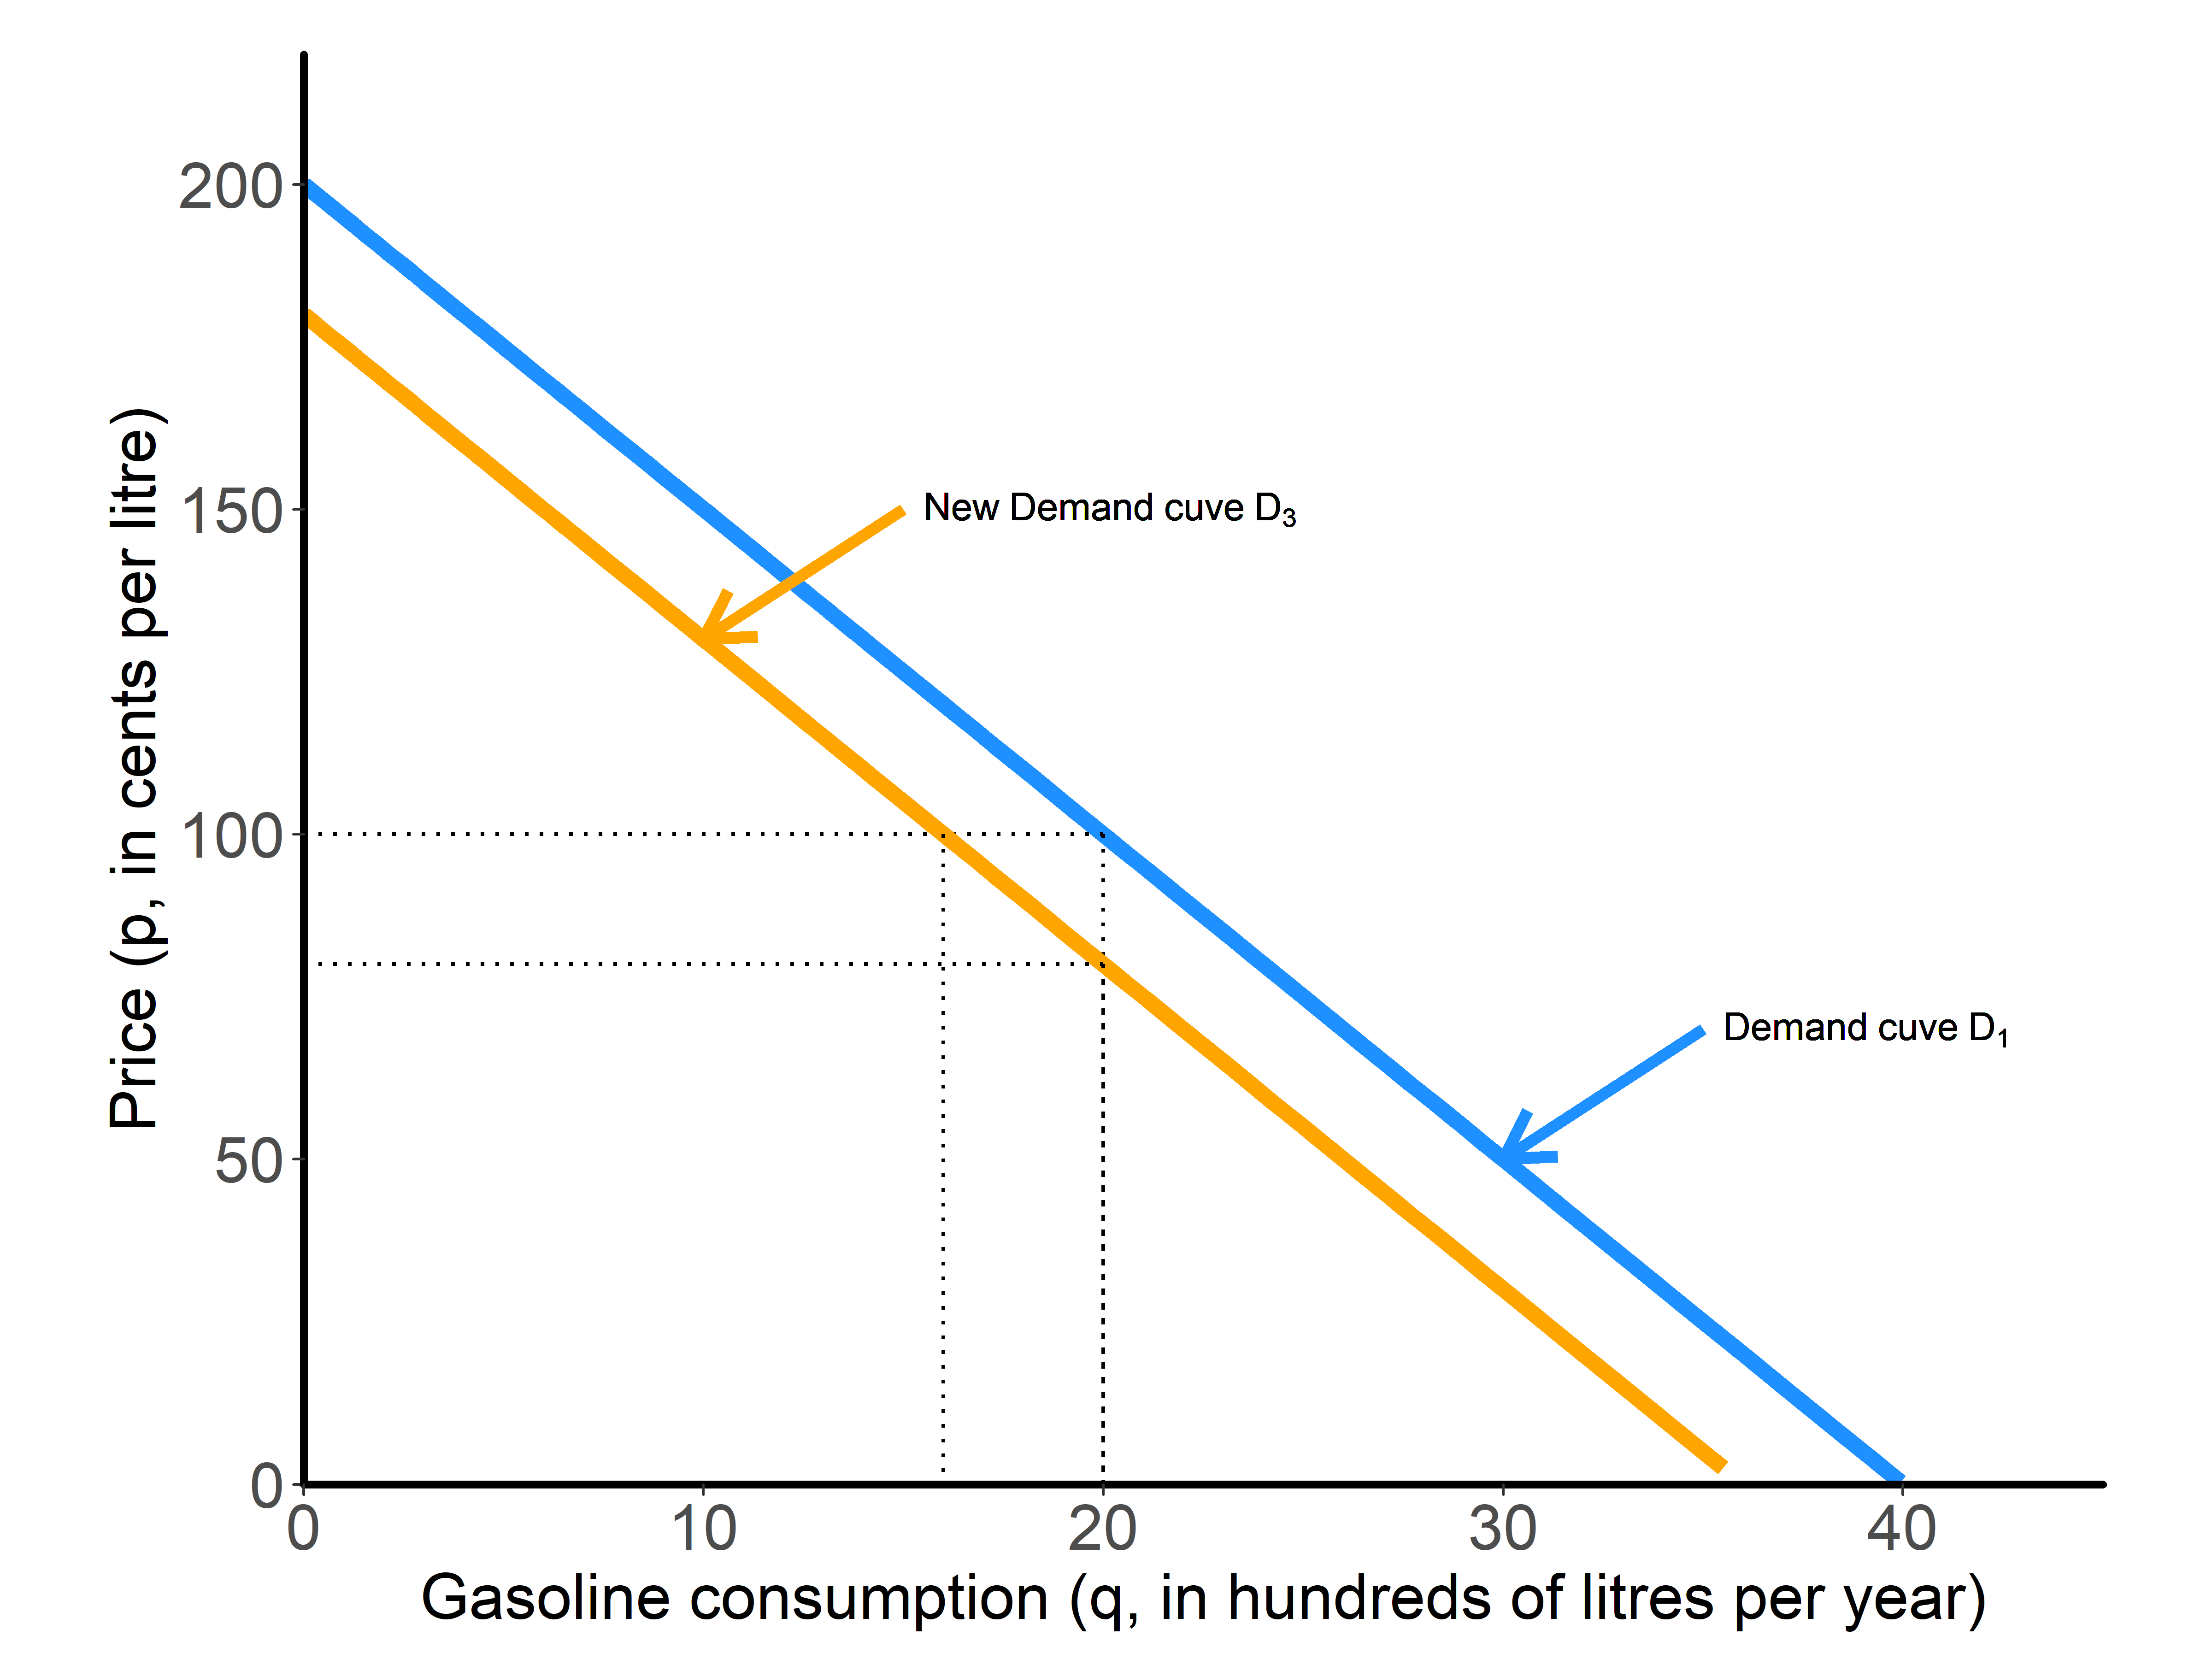
\includegraphics[width=\textwidth]{../images/gas_inc_comp.png}
}
\caption{The effects of an increase in the price of tolls on the demand for gasoline}
\end{figure}
}

\frame{
	\frametitle{The Demand Curve}
	%	The demand for gasoline:
	
		\begin{figure}[t!]
	\center
	\resizebox{!}{.45\linewidth}{
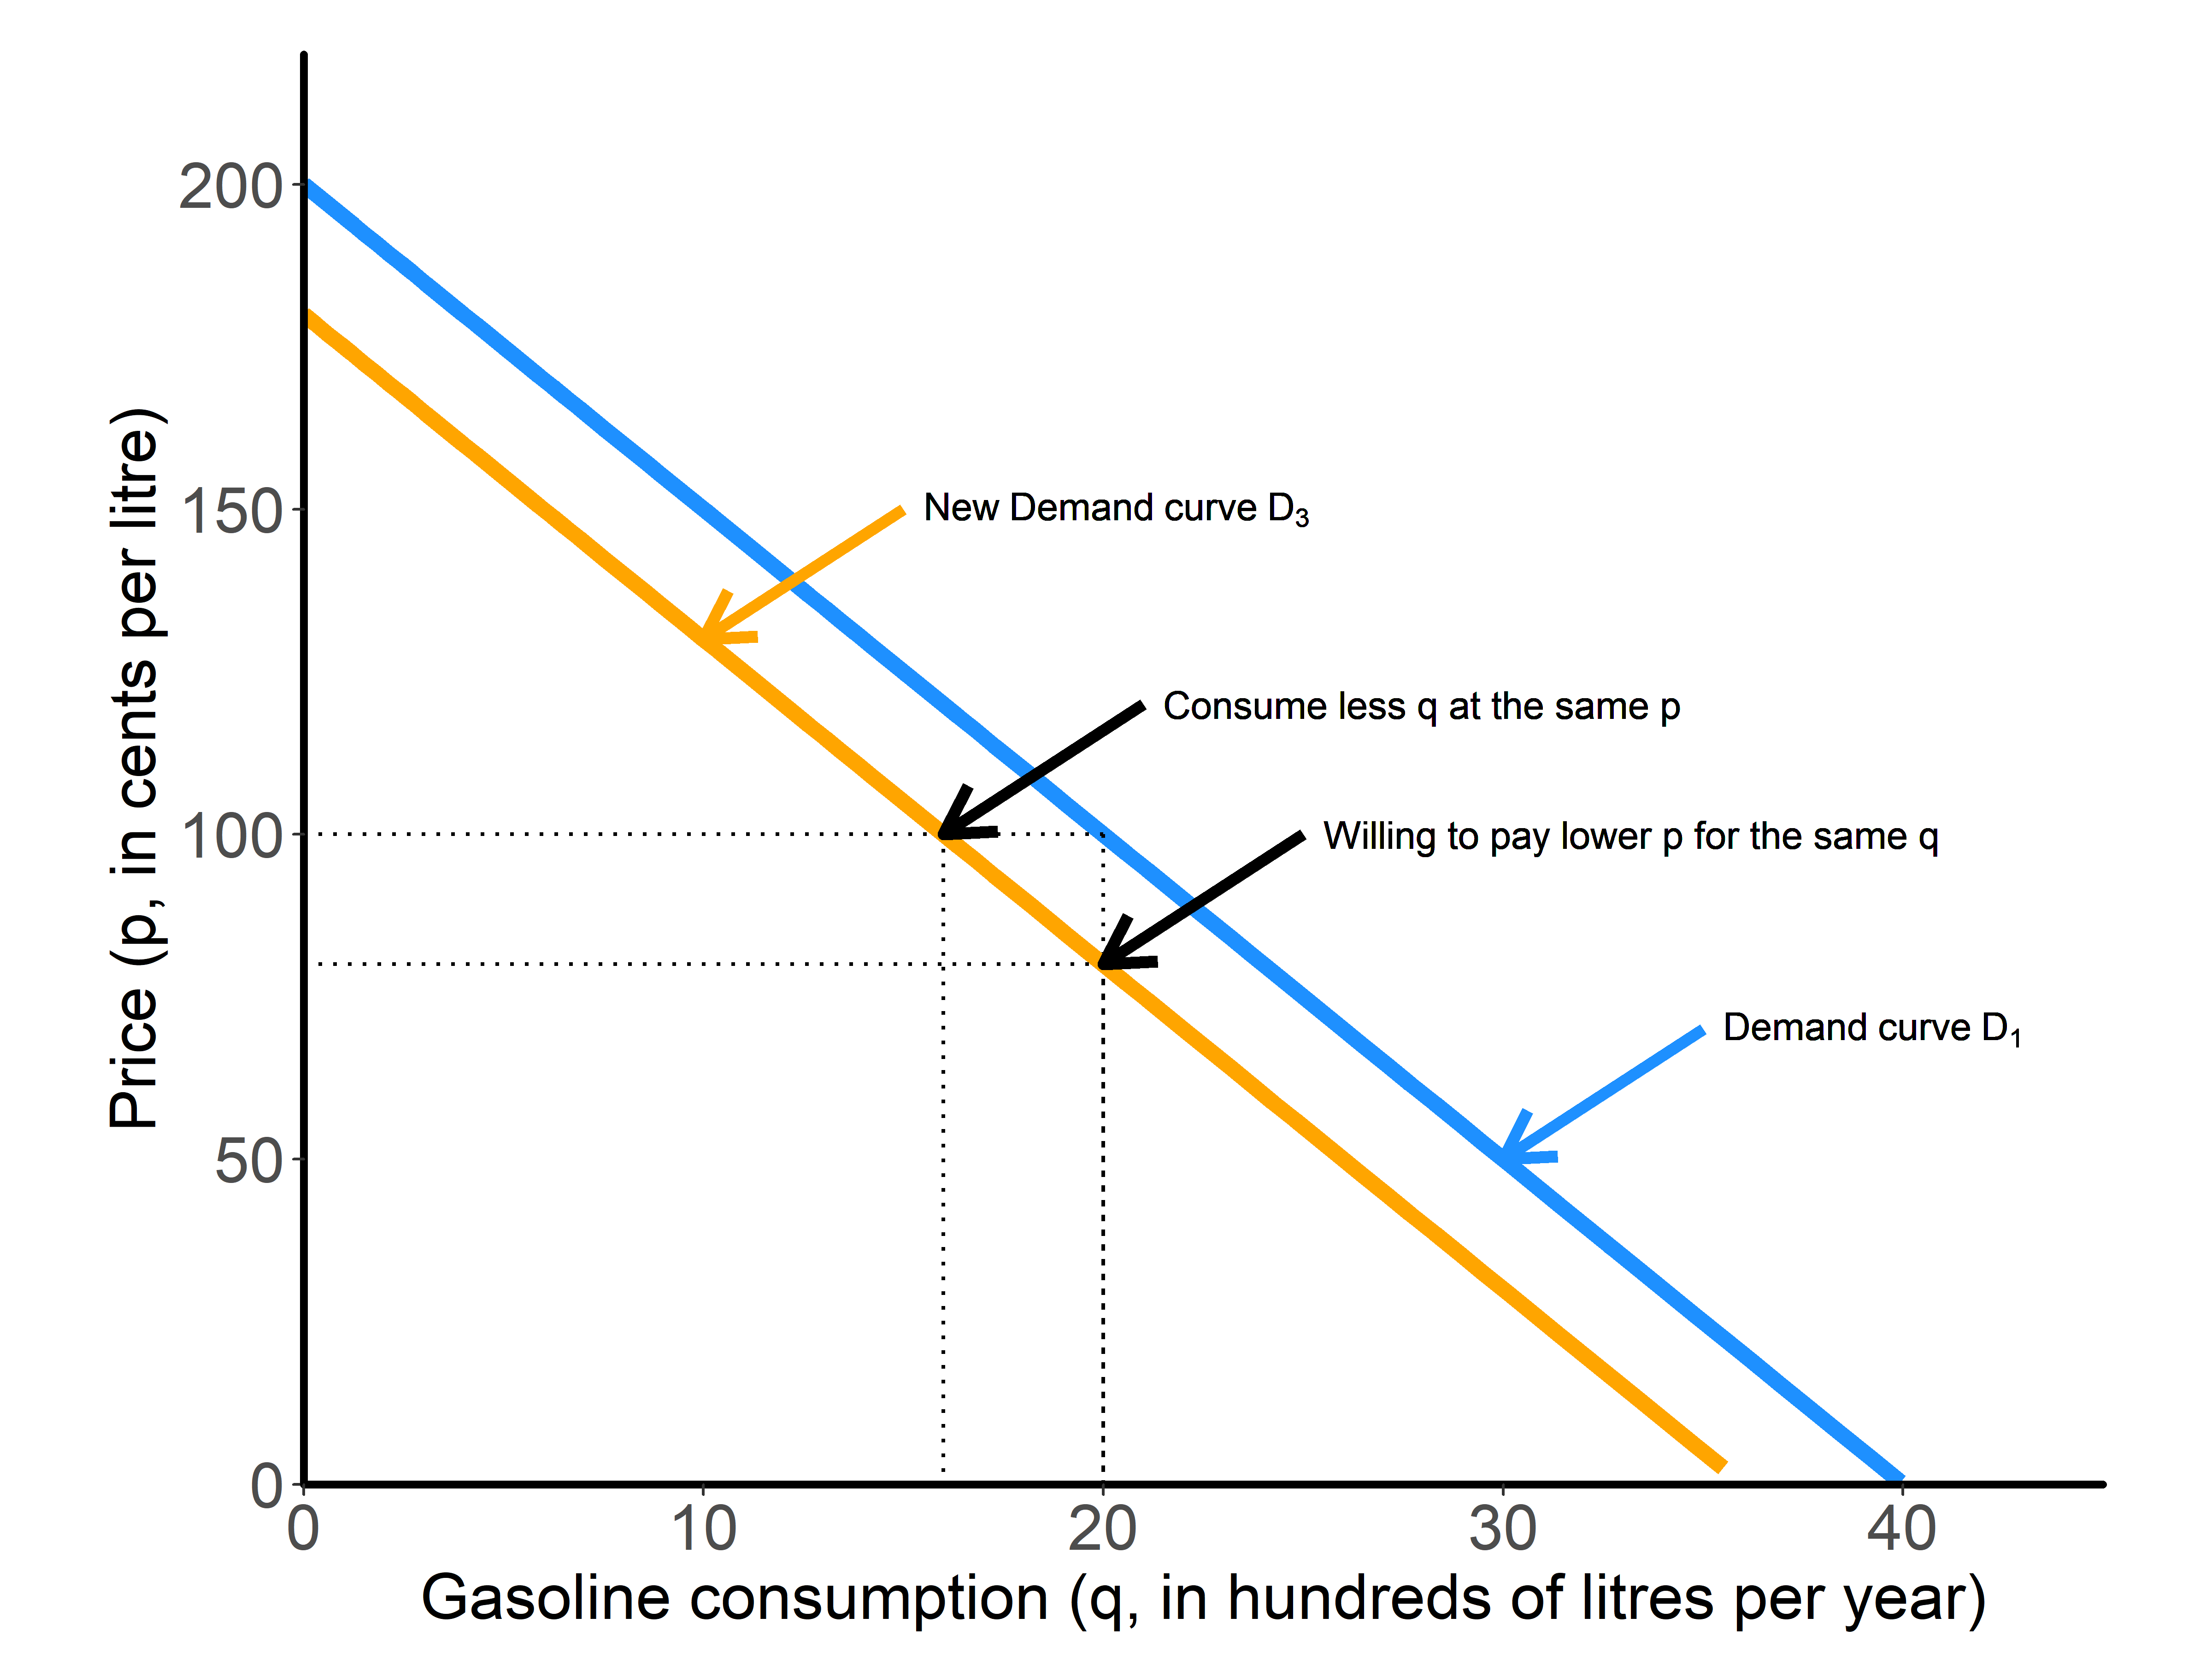
\includegraphics[width=\textwidth]{../images/gas_inc_comp2.png}
}
\caption{The effects of an increase in road tolls on the demand for gasoline}
\end{figure}
}



\frame{
	\frametitle{The Demand Curve}
	\begin{itemize}
	\item The demand curve gives us a precise relationship between price and quantity demanded.
	\item We can also express this same relationship mathematically using a \textit{demand function}.
	\item The demand function is given by:
		\begin{align*}
		Q = D(p,Y,X)
		\end{align*}
	where $Q$ is the quantity demanded, and $D(\cdot)$ is the demand function that depends on the price,
$p$, income, $Y$, and other factors, $X$.
	\item For simplicity, in what follows we will hold other factors ($X$) constant.
	\end{itemize}
}

\frame{
	\frametitle{The Demand Function}
	\begin{itemize}
	\item In the graphs above, I've used the equation
		\begin{align*}
		Q = 30 - \frac{p}{5} + 0.1 Y
		\end{align*}
	where $Q$ is the quantity of gasoline demanded, $p$ is the price of gasoline, and $Y$ is average
household income in thousands of dollars per year.
	\item[]
	\item Functional form reflects available evidence about the demand for gasoline:
		\begin{itemize}
		\item $p$ is negative.
		\item $Y$ is positive.
		\item Constant term ($30$) reflects all other factors.
		\end{itemize}
\item The parameters here ($30$,$\frac{1}{5}$, and $0.1$ aren't estimated, they are simply illustrative.
	\end{itemize}
}

\frame{
	\frametitle{The Demand Function}
	\begin{itemize}
	\item We can obtain the demand curve for gasoline by substituting for income, $Y$.
	\item If household income is \$100,000. the demand for gasoline is given by:
		\begin{align*}
		Q &= 30 - \frac{p}{5} + 0.1\times 100\\
        Q &= 40 - \frac{p}{5}
		\end{align*}
	\item With some algebra we can obtain the \textit{inverse demand curve}:
		\begin{align*}
		Q &= 40 - \frac{p}{5}\\
        5Q &= 200 - p\\
        p &= 200 -5Q
		\end{align*}
	\end{itemize}
}

\frame{
	\frametitle{The Demand Function}
	%	The demand for gasoline:

	\begin{figure}[t!]
	\center
	\resizebox{!}{.45\linewidth}{
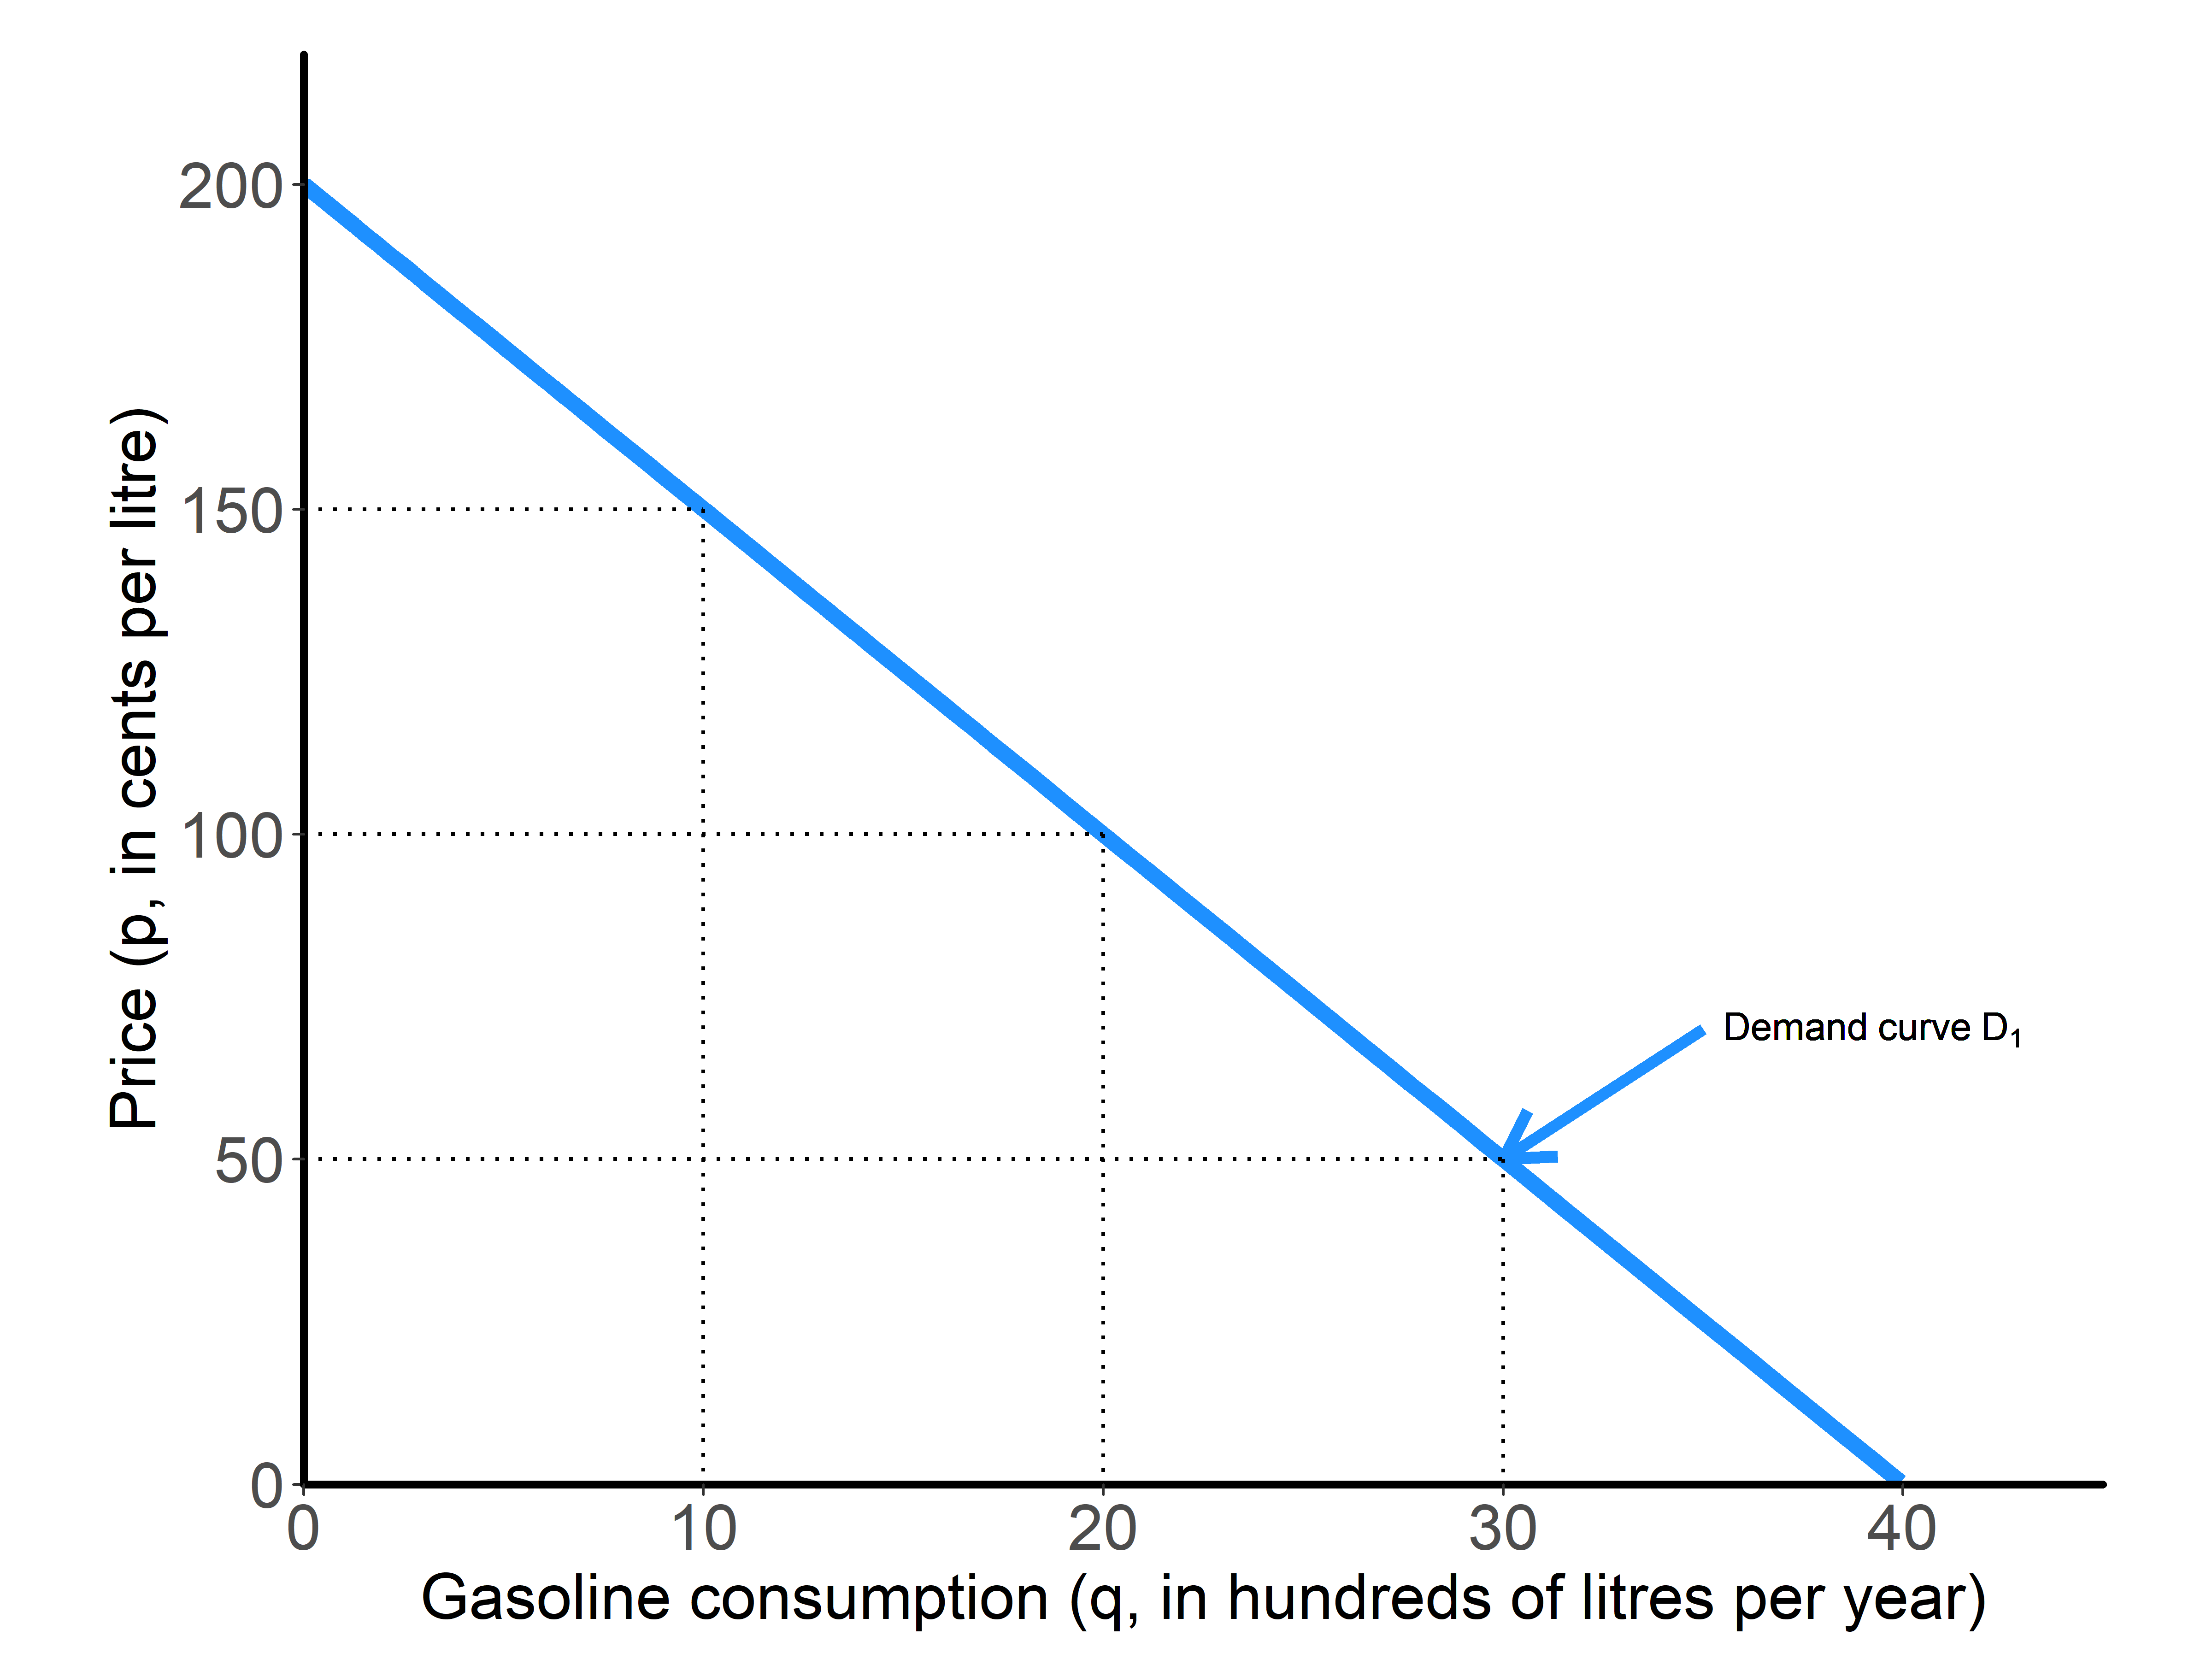
\includegraphics[width=\textwidth]{../images/gas_demand.png}
}
\caption{The demand for gasoline}
\end{figure}
}

\frame{
	\frametitle{The Demand Function}
	\begin{itemize}
	\item The demand function is useful because it allows us to think precisely about how the
quantity demanded will respond to a change in price, holding income (and all other factors) fixed.
\item To see this, let's use two of the (price,quantity) pairs highlighted by the dotted lines in the figure:
\begin{itemize}
\item Let $p_{1}=100$ denote the initial price, and $p_{2}=50$ denote the new price.
\item The quantity demanded at $p_{1}$ is $Q_{1}=D(p_{1})=40-\frac{p_1}{5}=40-\frac{100}{5}=20$ \medskip
\item The quantity demanded at $p_{2}$ is $Q_{2}=D(p_{2})=40-\frac{p_2}{5}
=40-\frac{50}{5}=30$
\end{itemize}
\item Next we can use these to start thinking about response to price changes
\end{itemize}
}



\frame{
	\frametitle{The Demand Function}
	\begin{itemize}
\item In our gasoline example, if the price changes from $p_{1}$ to $p_{2}$, the change in
quantity demanded is given by:
		\begin{align*}
		\Delta Q &= D(p_{2})-D(p_{1}) = [40-\frac{p_2}{5}]-[40-\frac{p_1}{5}]\\
        \Delta Q &= D(p_{2})-D(p_{1}) = \frac{p_1}{5}-\frac{p_2}{5}\\
        \Delta Q &= D(p_{2})-D(p_{1}) = -\frac{1}{5}\Delta P,\,\Delta P=p_{2}-p_{1}
		\end{align*}
\item So, we know that for a given change in price $\Delta P$, the quantity consumed will change by
 $\Delta Q=-\frac{1}{5}\Delta P$
 	\end{itemize}	
}


\frame{
	\frametitle{The Demand Function}
	\begin{itemize}
\item How do we see this? Check the graph:
\begin{center}
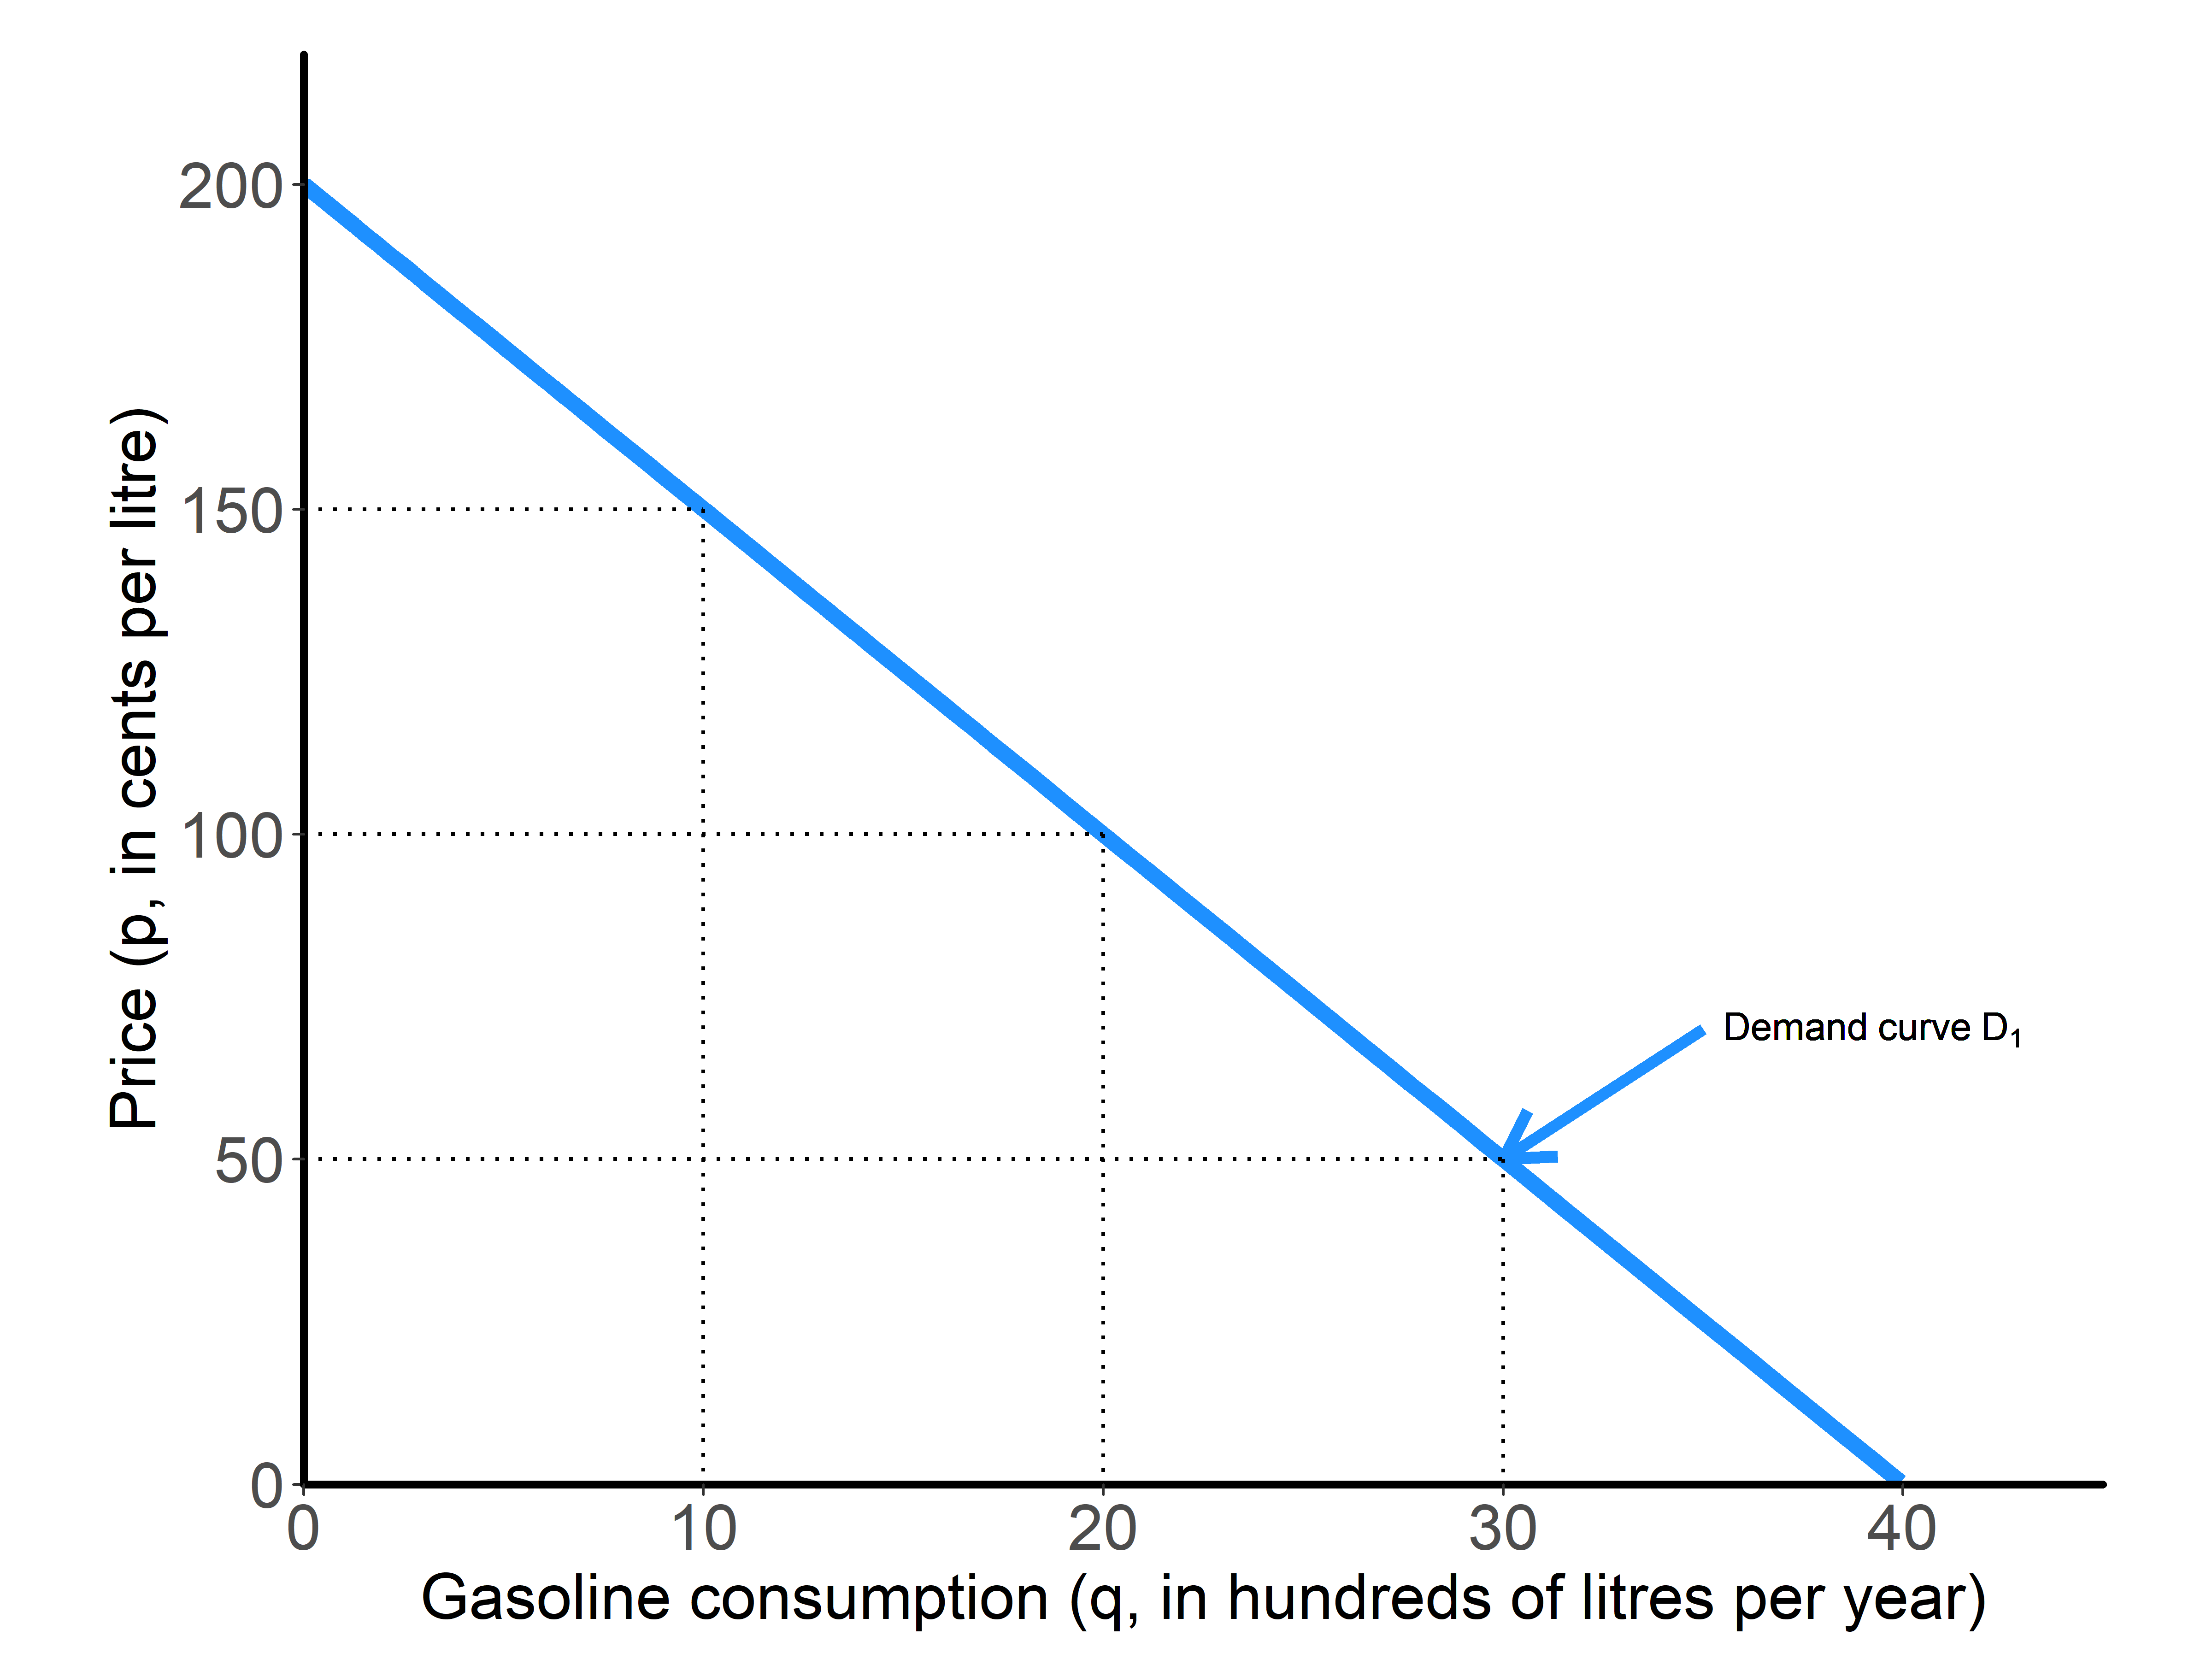
\includegraphics[width=.4\textwidth]{../images/gas_demand.png}
\end{center}
\item Changing the price from 50 to 100 decreases Q from 30 to 20, so $\Delta Q=-10$
\item From the previous slide, $\Delta Q=-\frac{1}{5}\Delta P=-\frac{50}{5}=-10$
 	\end{itemize}	
}



\frame{
	\frametitle{Market Demand}
	\begin{itemize}
	\item In many cases we might have an estimate of the demand from all consumers in a market, but
in some scenarios, we may only know the demands of individual consumers or groups of consumers.
	\item[]
	\item In these cases, we need to add up the demand from each consumer (or group).
	\item[]
	\item \alert{Key point}: Total quantity demanded \textit{at a given price} is equal to the sum of
individual consumer demands \alert{at that price}.
	\end{itemize}
}

\frame{
	\frametitle{Determining Market Demand}
	\begin{itemize}
	\item As an example, suppose there are two people in the market for gasoline. They both have
demand functions given by:
		\begin{align*}
		Q=40-\frac{p}{5}
		\end{align*}
		What is the market demand for gasoline in this case?
	\end{itemize}
}


\frame{
	\frametitle{Determining Market Demand}
	\begin{itemize}
\item Again, check the graph to find yourself an easy anchor point:
\begin{center}
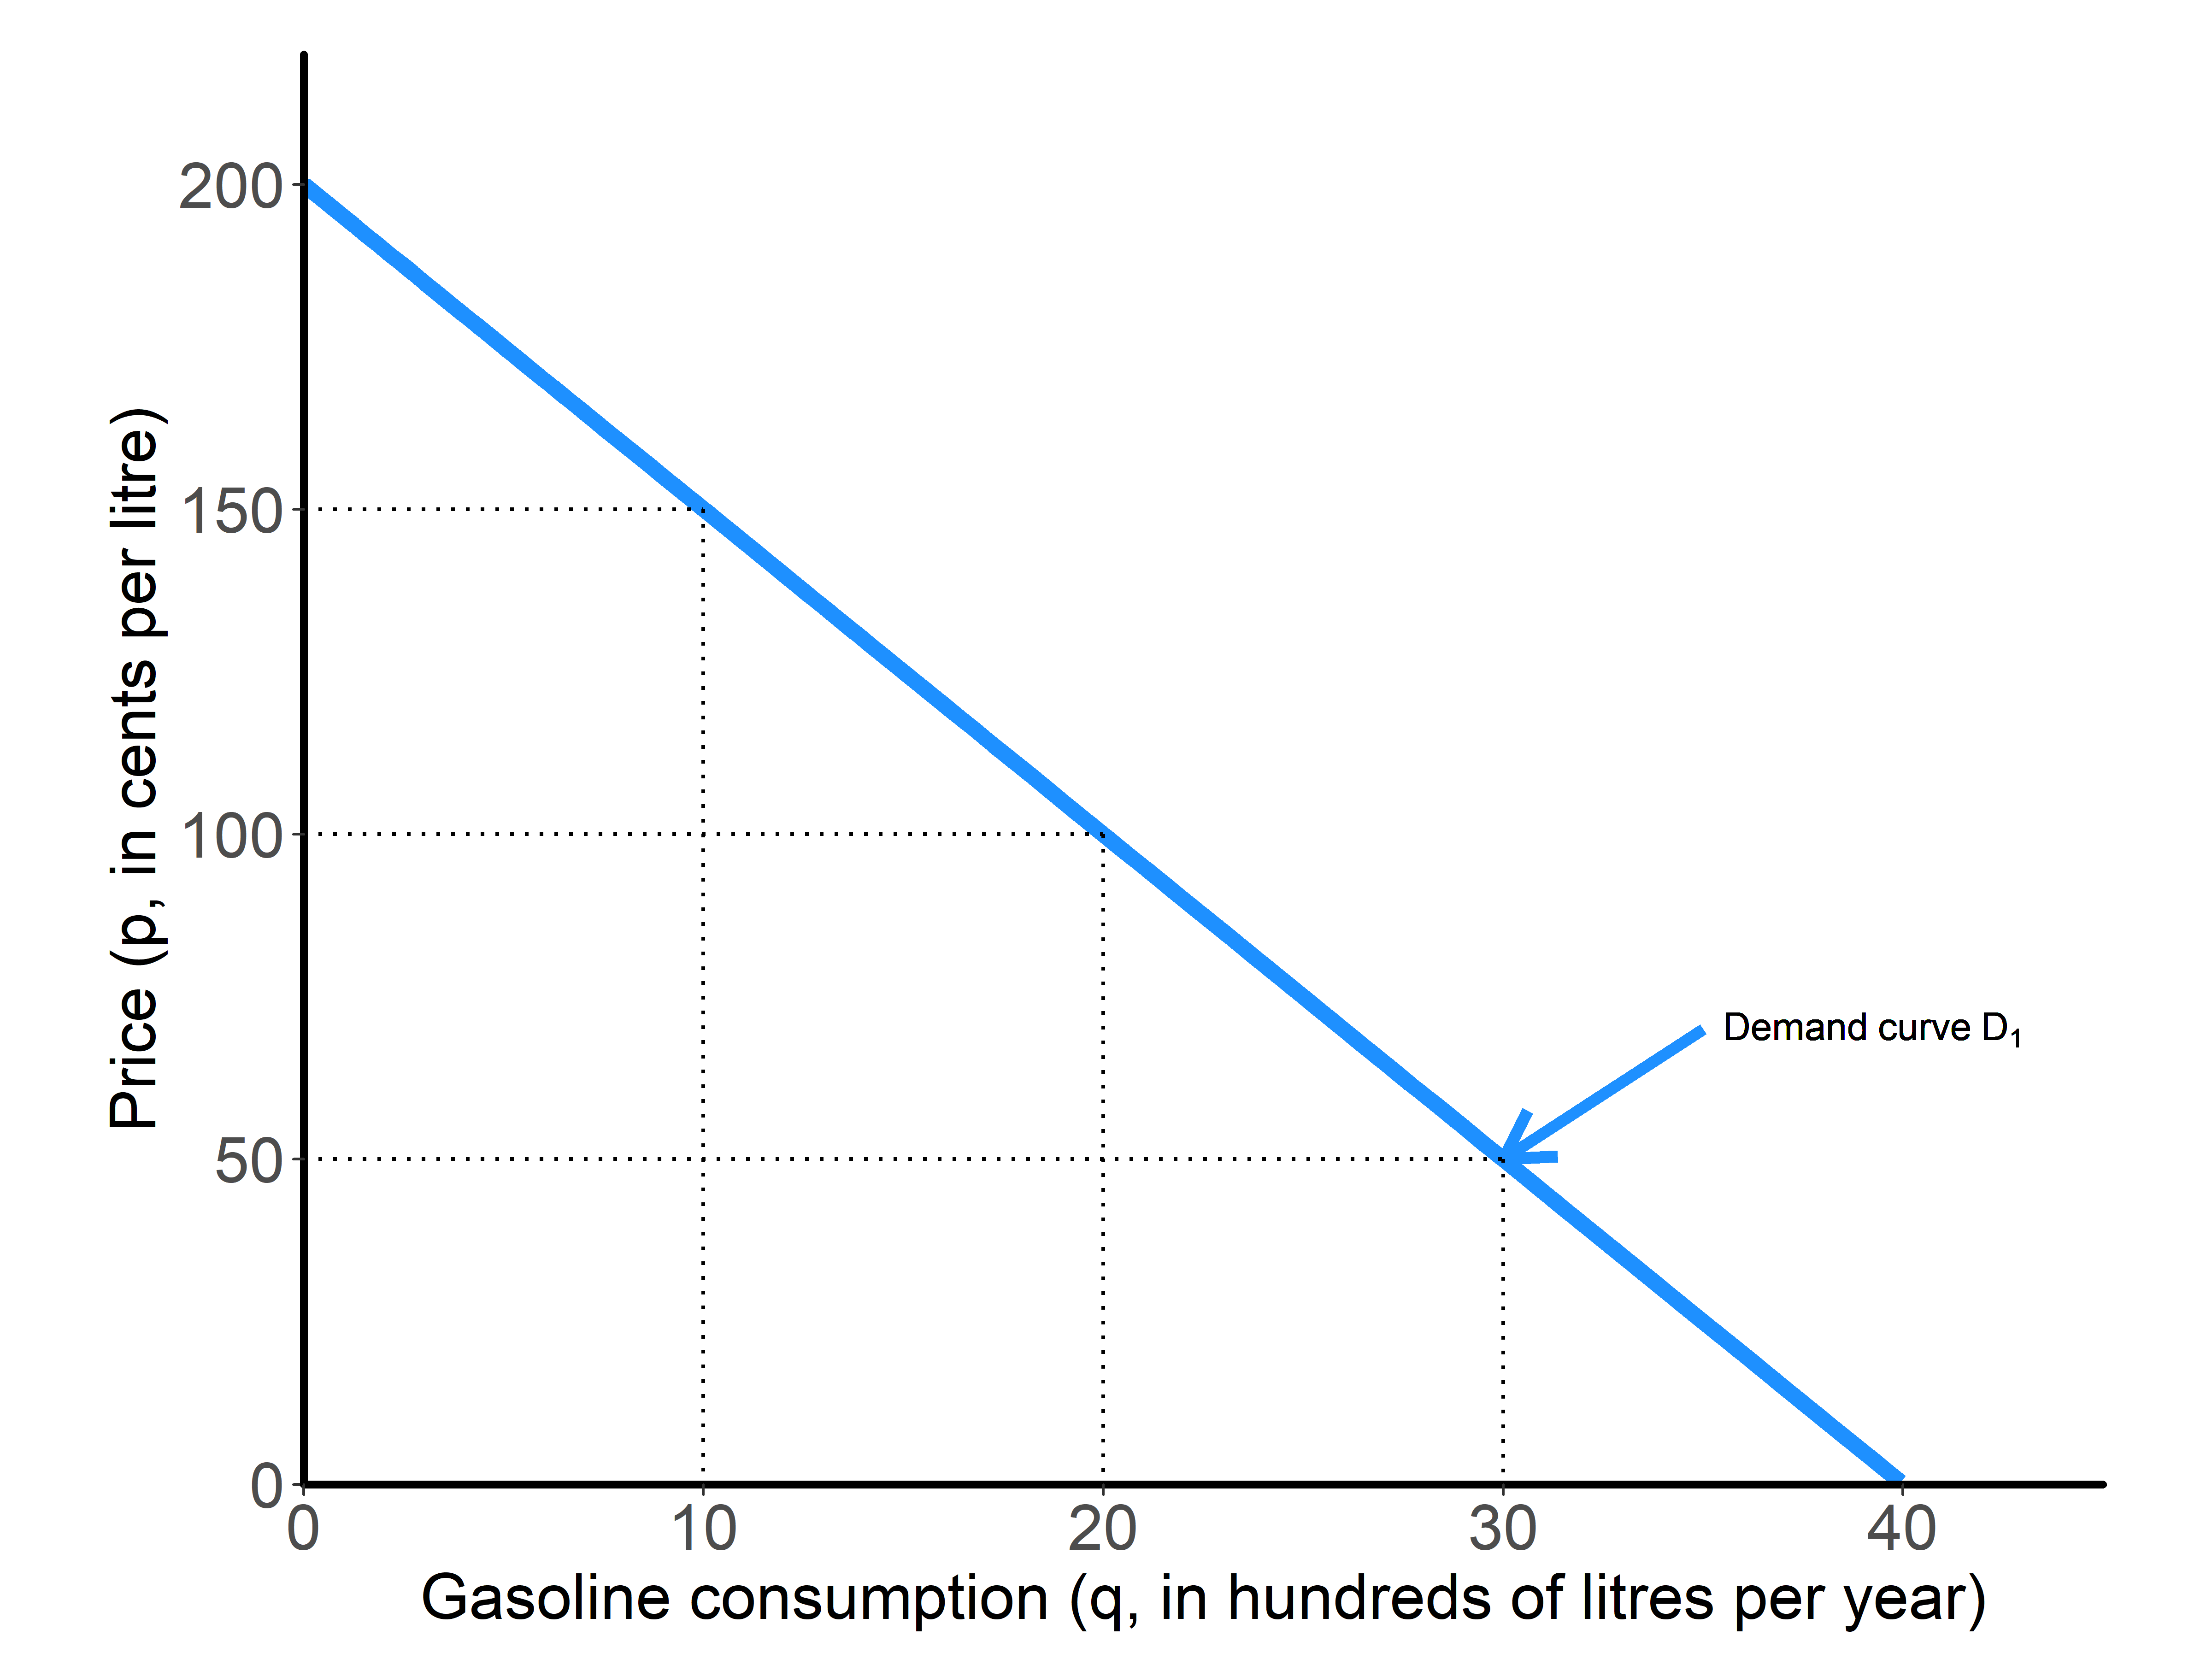
\includegraphics[width=.4\textwidth]{../images/gas_demand.png}
\end{center}
\item What's the demand from one person at price p=100? It's 20.
\item So, if the demand from one person at price p=100 is 20, what's the demand from 2 people?
 	\end{itemize}	
}


\frame{
	\frametitle{Determining Market Demand}
	\begin{itemize}
\item Okay, now let's do the math:\\
\begin{center}
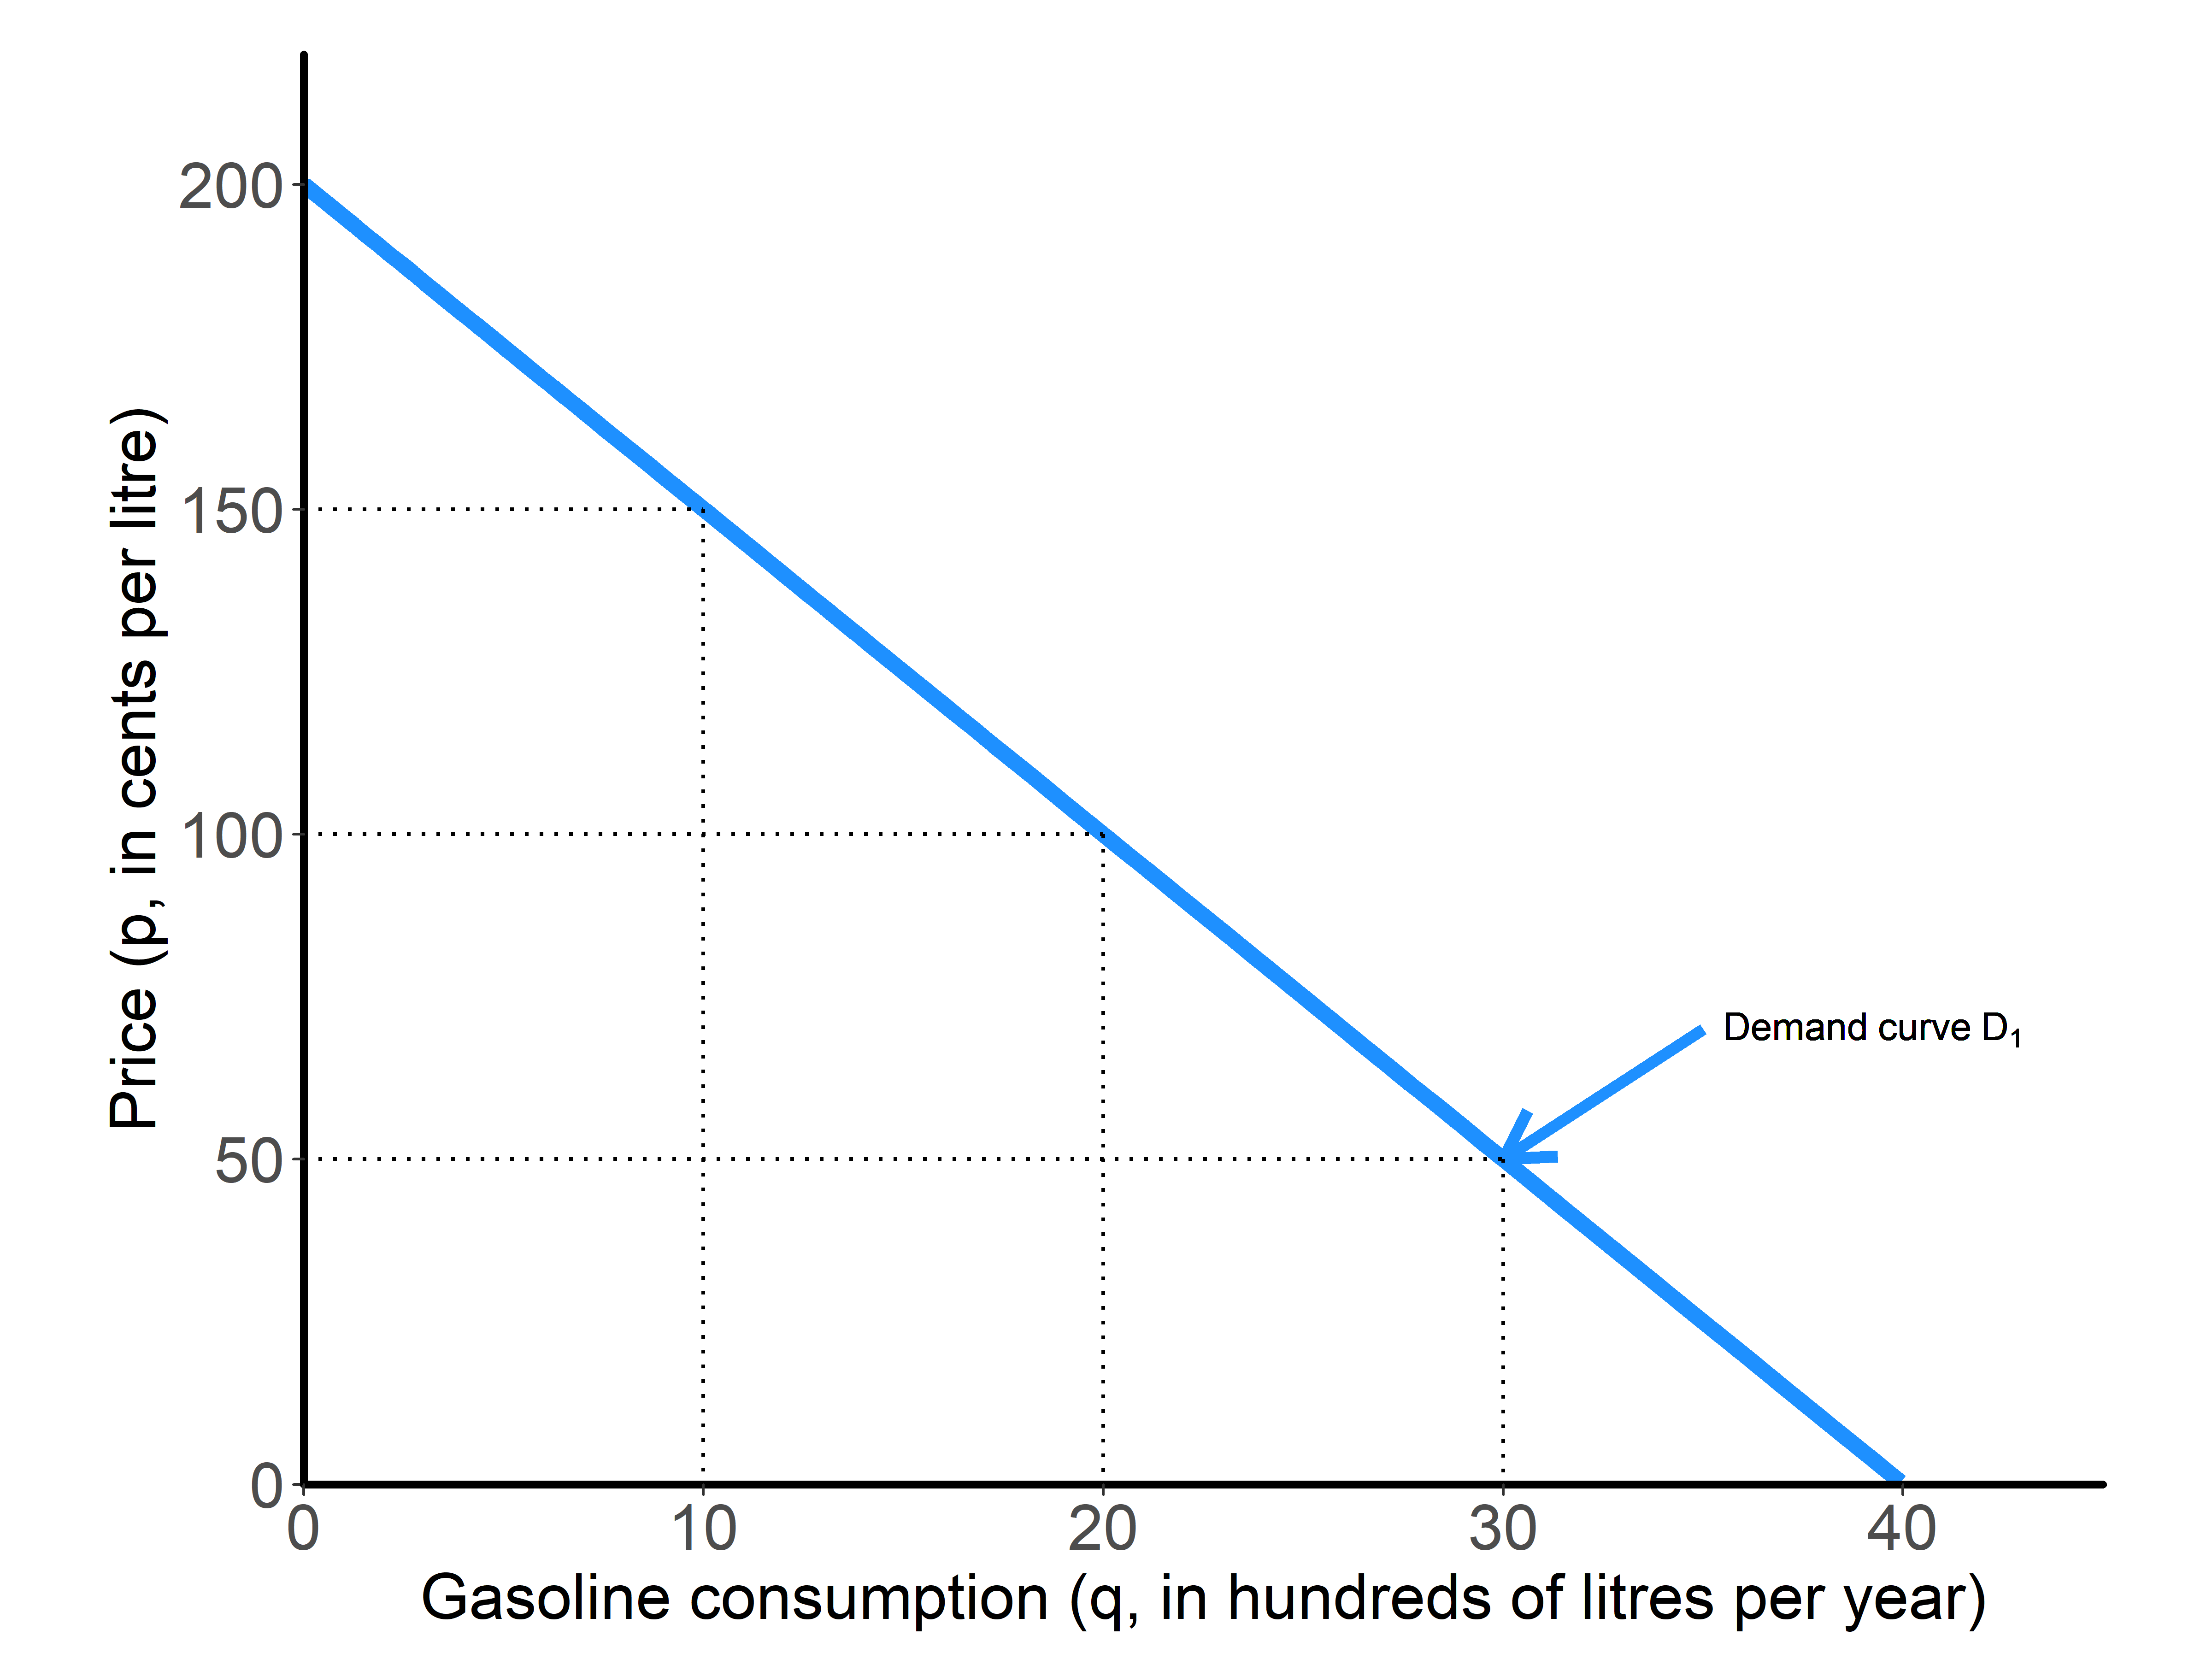
\includegraphics[width=.35\textwidth]{../images/gas_demand.png}
\end{center}
\item If $Q=40-\frac{p}{5}$, adding both sides of two demand functions yields $Q_m=80-\frac{2\times p}{5}$, where $Q_m$, the market demand, is twice individual demand.
\item Now let's check. If $p = 100$, $Q=80-\frac{2\times p}{5}=80-\frac{2\times 100}{5}=40$, which is twice the individual demand at that price - I've done the math correctly.
 	\end{itemize}	
}

\frame{
	\frametitle{Determining Market Demand}
	%	The demand for gasoline:

	\begin{figure}[t!]
	\center
	\resizebox{!}{.45\linewidth}{
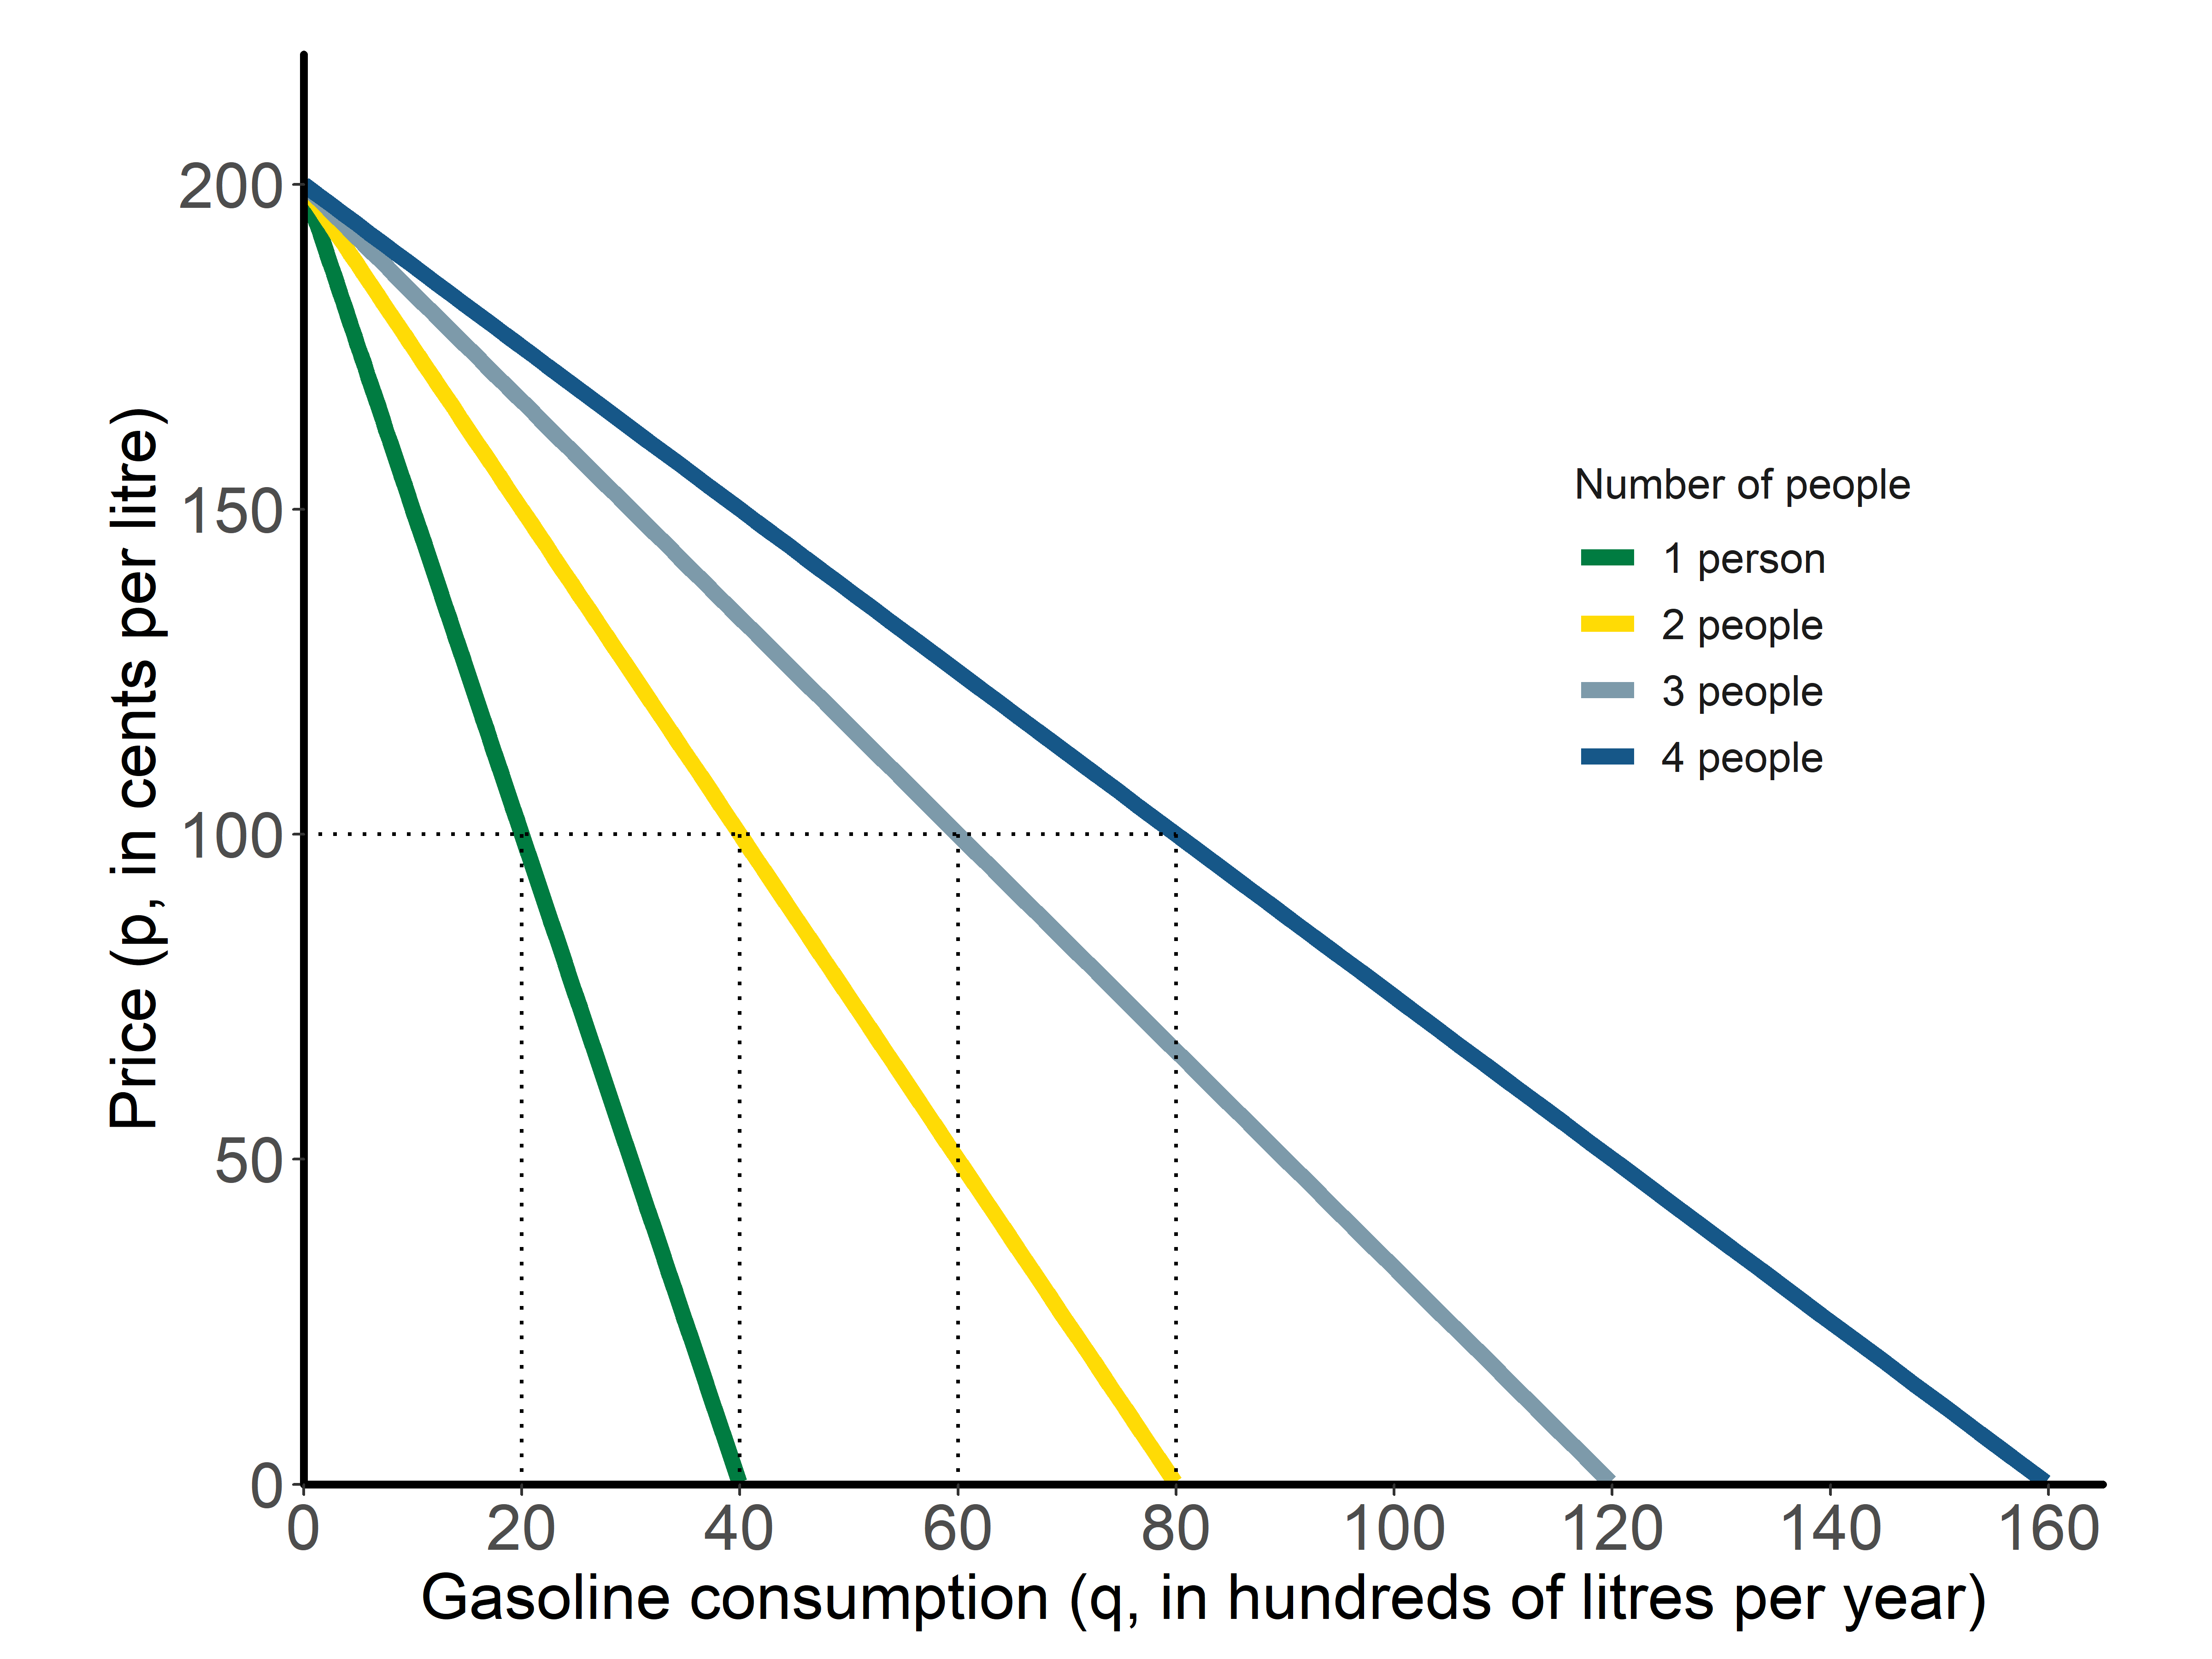
\includegraphics[width=\textwidth]{../images/gas_stack.png}
}
\caption{The demand for gasoline aggregated for 1, 2, 3 or 4 people}
\end{figure}
}

\frame{
	\frametitle{Determining Market Demand}
\begin{definition}[Horizontal Summation]
		When summing demand for a \textit{private good}, you add up the quantity demanded of each individual at each price.

\textbf{Trap: don't look at the graph and add the curves vertically. Just remember, if no one person demands gasoline above price $p_max$, the market doesn't demand any at prices above $p_max$ either}.
		\end{definition}

}

\frame{
	\frametitle{Determining Market Demand}
Test yourself: what's the aggregate demand in this case?
\begin{figure}[t!]
	\center
	\resizebox{!}{.4\linewidth}{
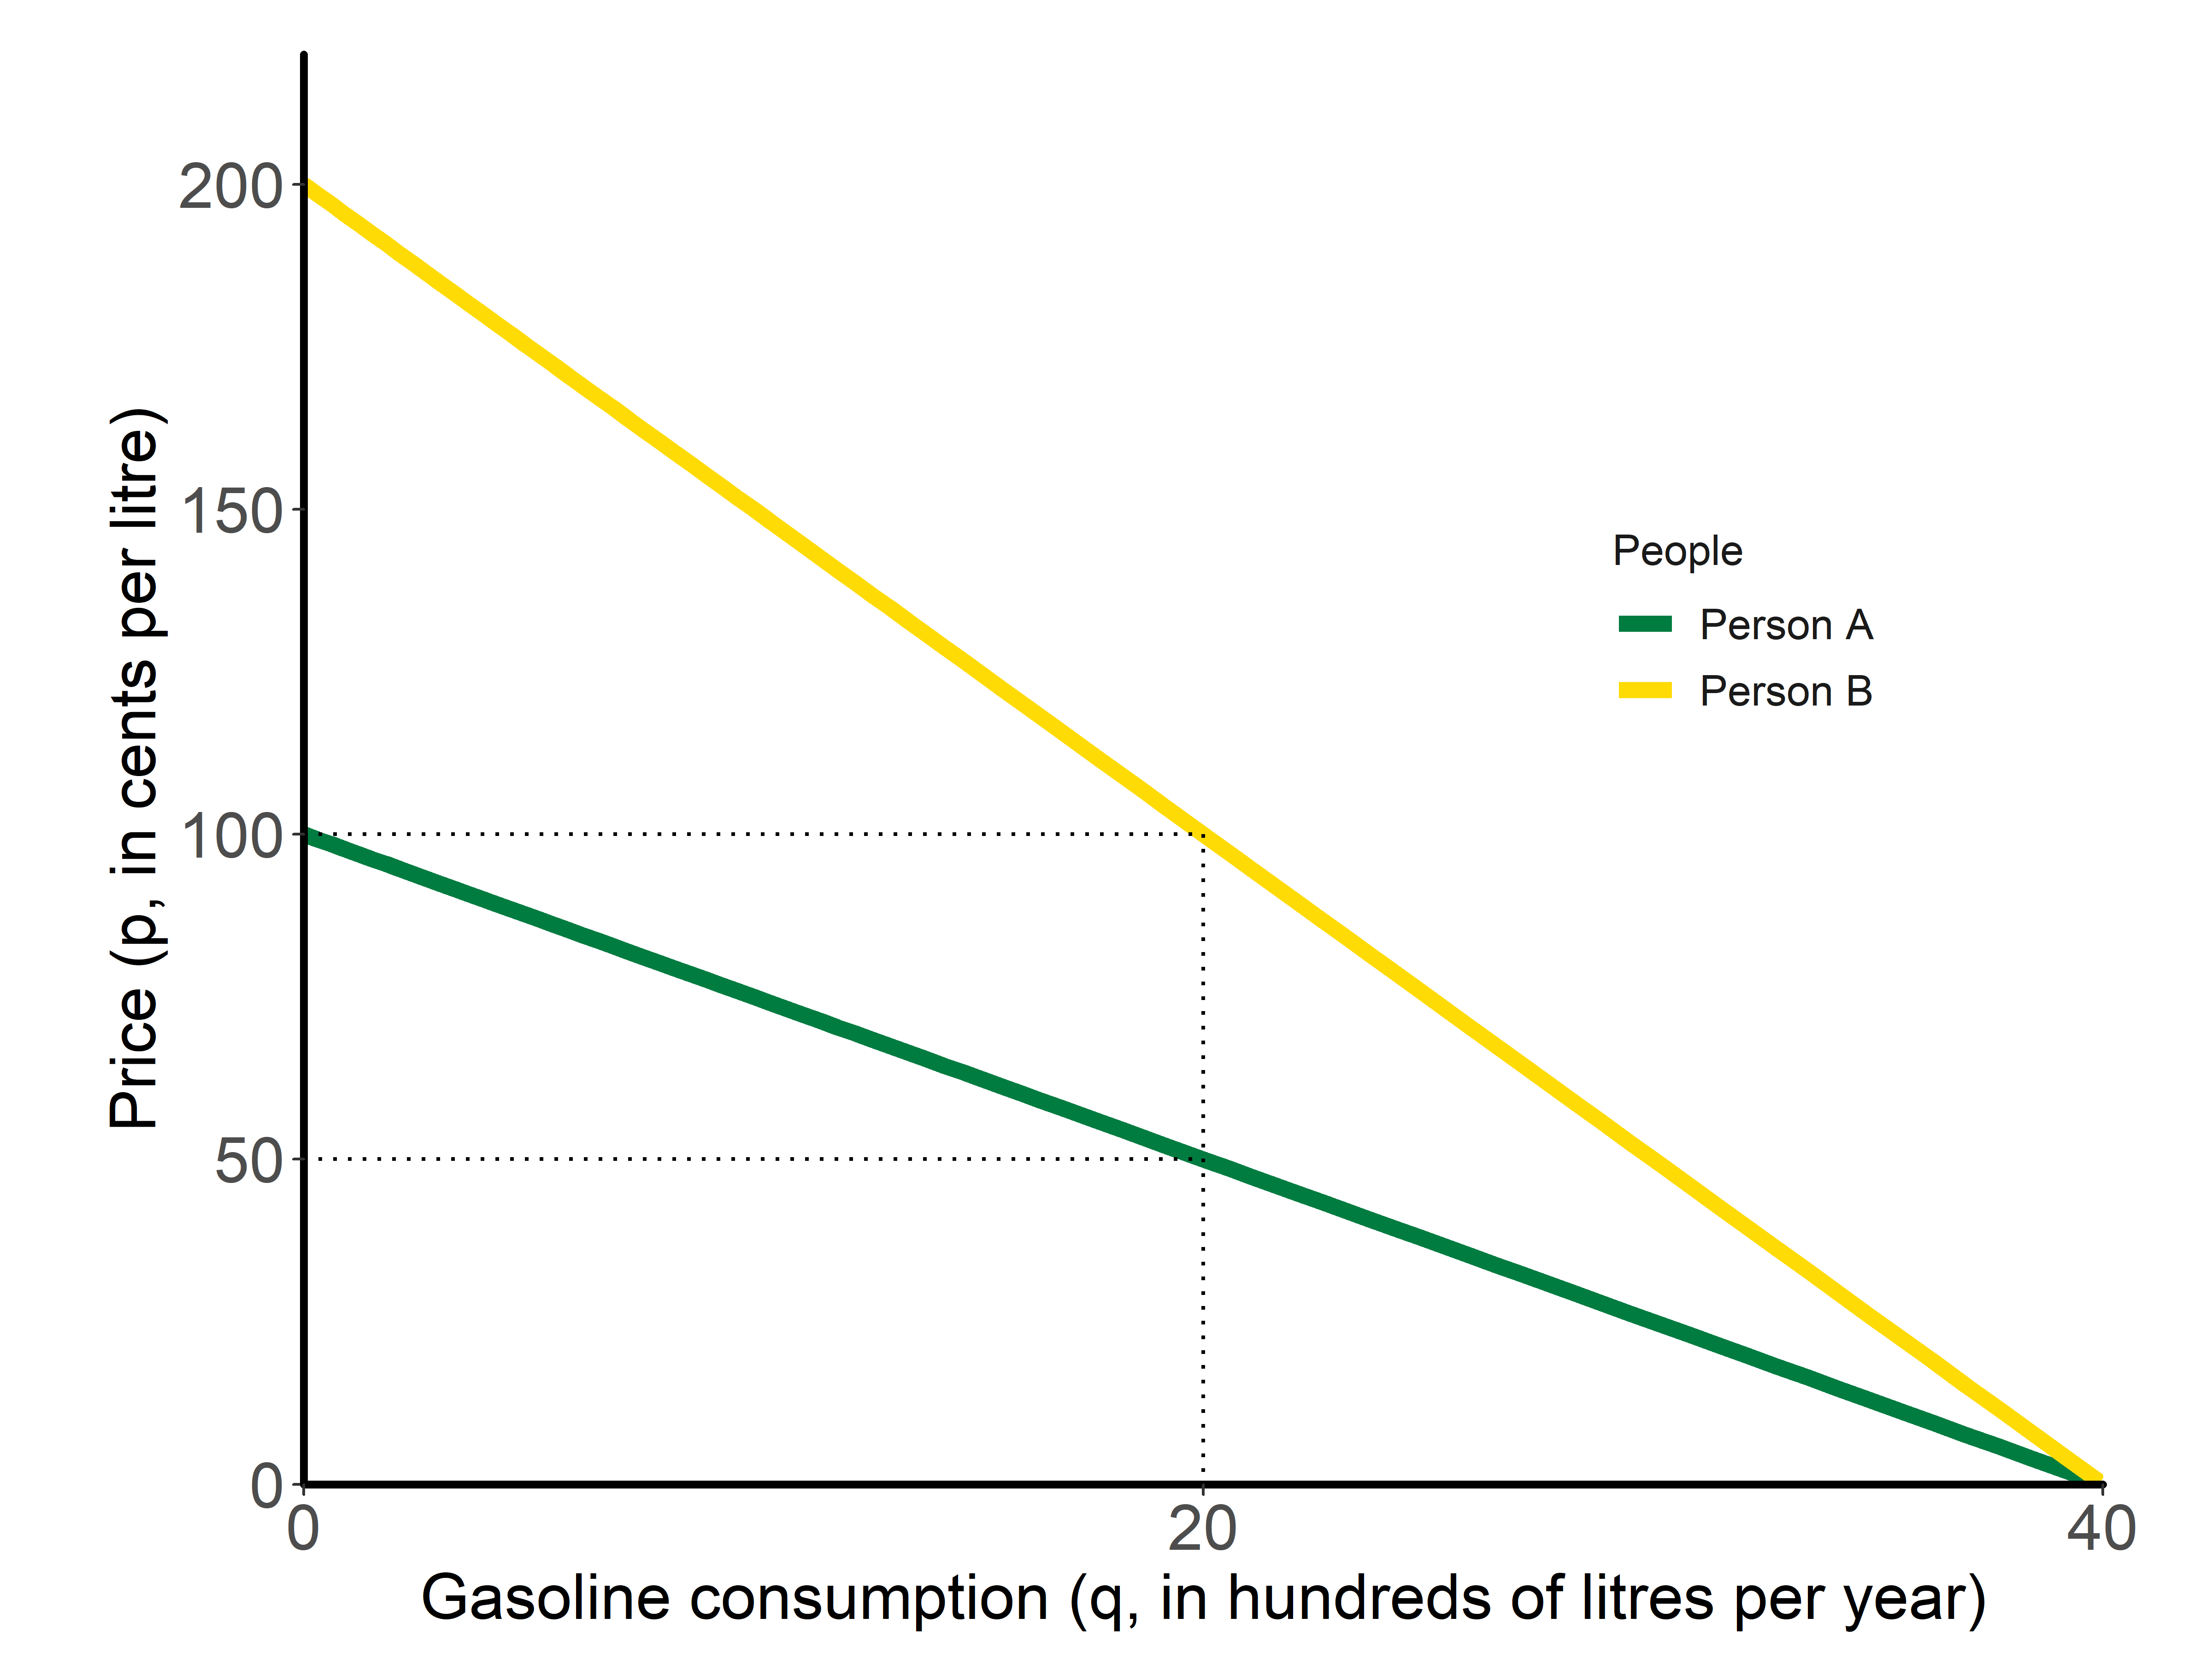
\includegraphics[width=\textwidth]{../images/gas_stack2a.png}
}
\caption{The demand for gasoline}
\end{figure}

}


%\end{document}

\section{Supply}

\frame{
	\frametitle{Supply}
	\begin{itemize}
	\item The second piece of the model: \textbf{Supply}
	\item[]
	\item Supply is producers' willingness to sell goods and services.
	\item[]
	\item What factors affect this willingness? How?
	\end{itemize}	
}

\frame{
	\frametitle{Supply}
	\begin{itemize}
	\item As with demand, economists focus on how the \textit{price} of a good or service affects the
quantity supplied.
	\end{itemize}
	\begin{definition}[Quantity Supplied]
	The amount of a good or service that producers \textit{want} to sell at a given price,
\textit{holding other factors that influence supply decisions constant}.
	\end{definition}
}

\frame{
	\frametitle{Supply}
	\begin{itemize}
	\item Is there a Law of Supply?
	\item[]
	\item We can illustrate the relationship between the price of a good or service and the quantity producers want to sell via a \textit{supply curve}.
	\end{itemize}
}

\frame{
	\frametitle{The Supply Curve}
	%	The demand for gasoline:
	\begin{figure}[t!]
	\center
	\resizebox{!}{.4\linewidth}{
    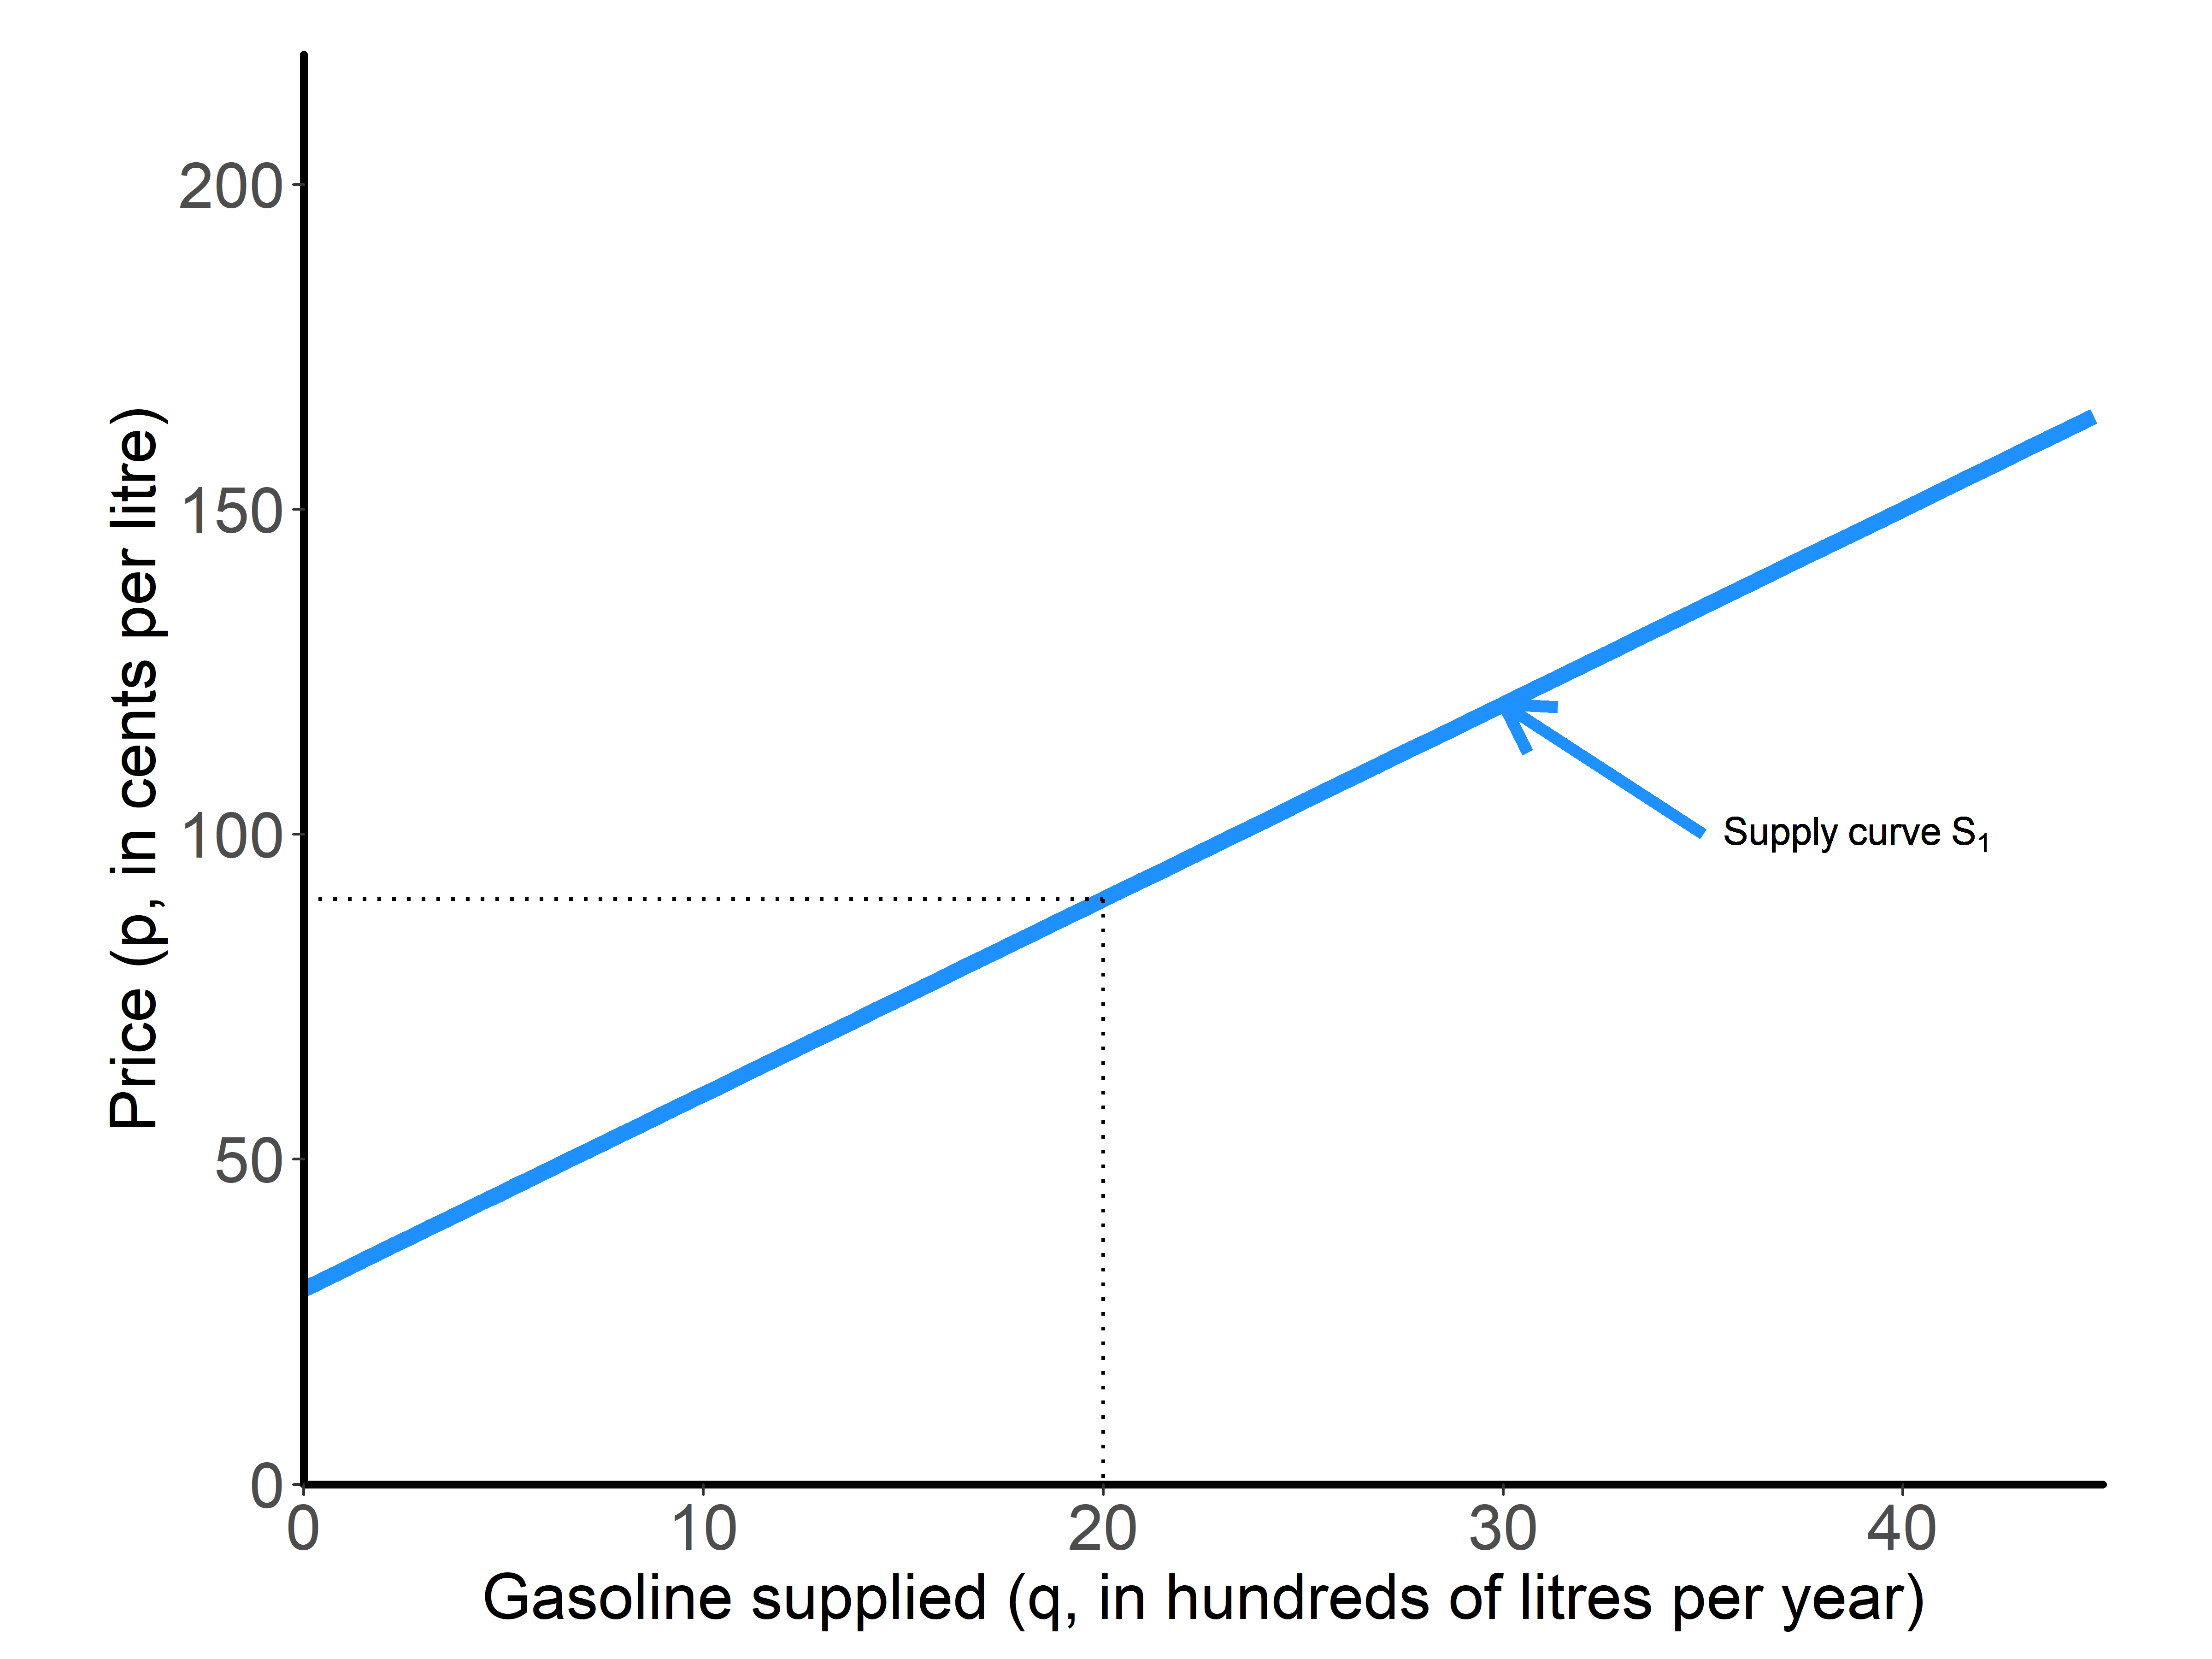
\includegraphics[width=\textwidth]{../images/gas_supply.png}
}
\caption{The supply of gasoline}
\end{figure}
}

\frame{
	\frametitle{The Supply Curve}
	\begin{itemize}
	\item The supply curve provides us an answer to the question of what happens to the quantity
supplied as price changes, holding all other factors fixed.
		\begin{itemize}
		\item Here: what happens to the supply of gasoline as the price of gasoline increases or
decreases.
		\end{itemize}
	\item[]
	\item Changes in the quantity supplied in response to a price change are referred to as
\textit{movements along the supply curve}.
	\item[]
	\item Do supply curves always need to slope upward?
	\end{itemize}
}

\frame{
	\frametitle{The Supply Curve}
	\begin{itemize}
	\item The supply curve tells us how a change in the price of a good or service affects the
quantity supplied.
		\begin{itemize}
		\item Change in $p$ $\implies$ \textit{movement along the supply curve}.
		\end{itemize}
	\item[]
	\item Recall that other factors also affect the quantity supplied.
		\begin{itemize}
		\item Change in these factors $\implies$ shift of the supply curve.
		\end{itemize}
	\item[]
	\item As an example, let's suppose that the price of the key input to gasoline production, crude oil, increases.
	\end{itemize}
}

\frame{
	\frametitle{The Supply Curve}
	%	The demand for gasoline:
	
	\begin{figure}[t!]
	\center
	\resizebox{!}{.4\linewidth}{
    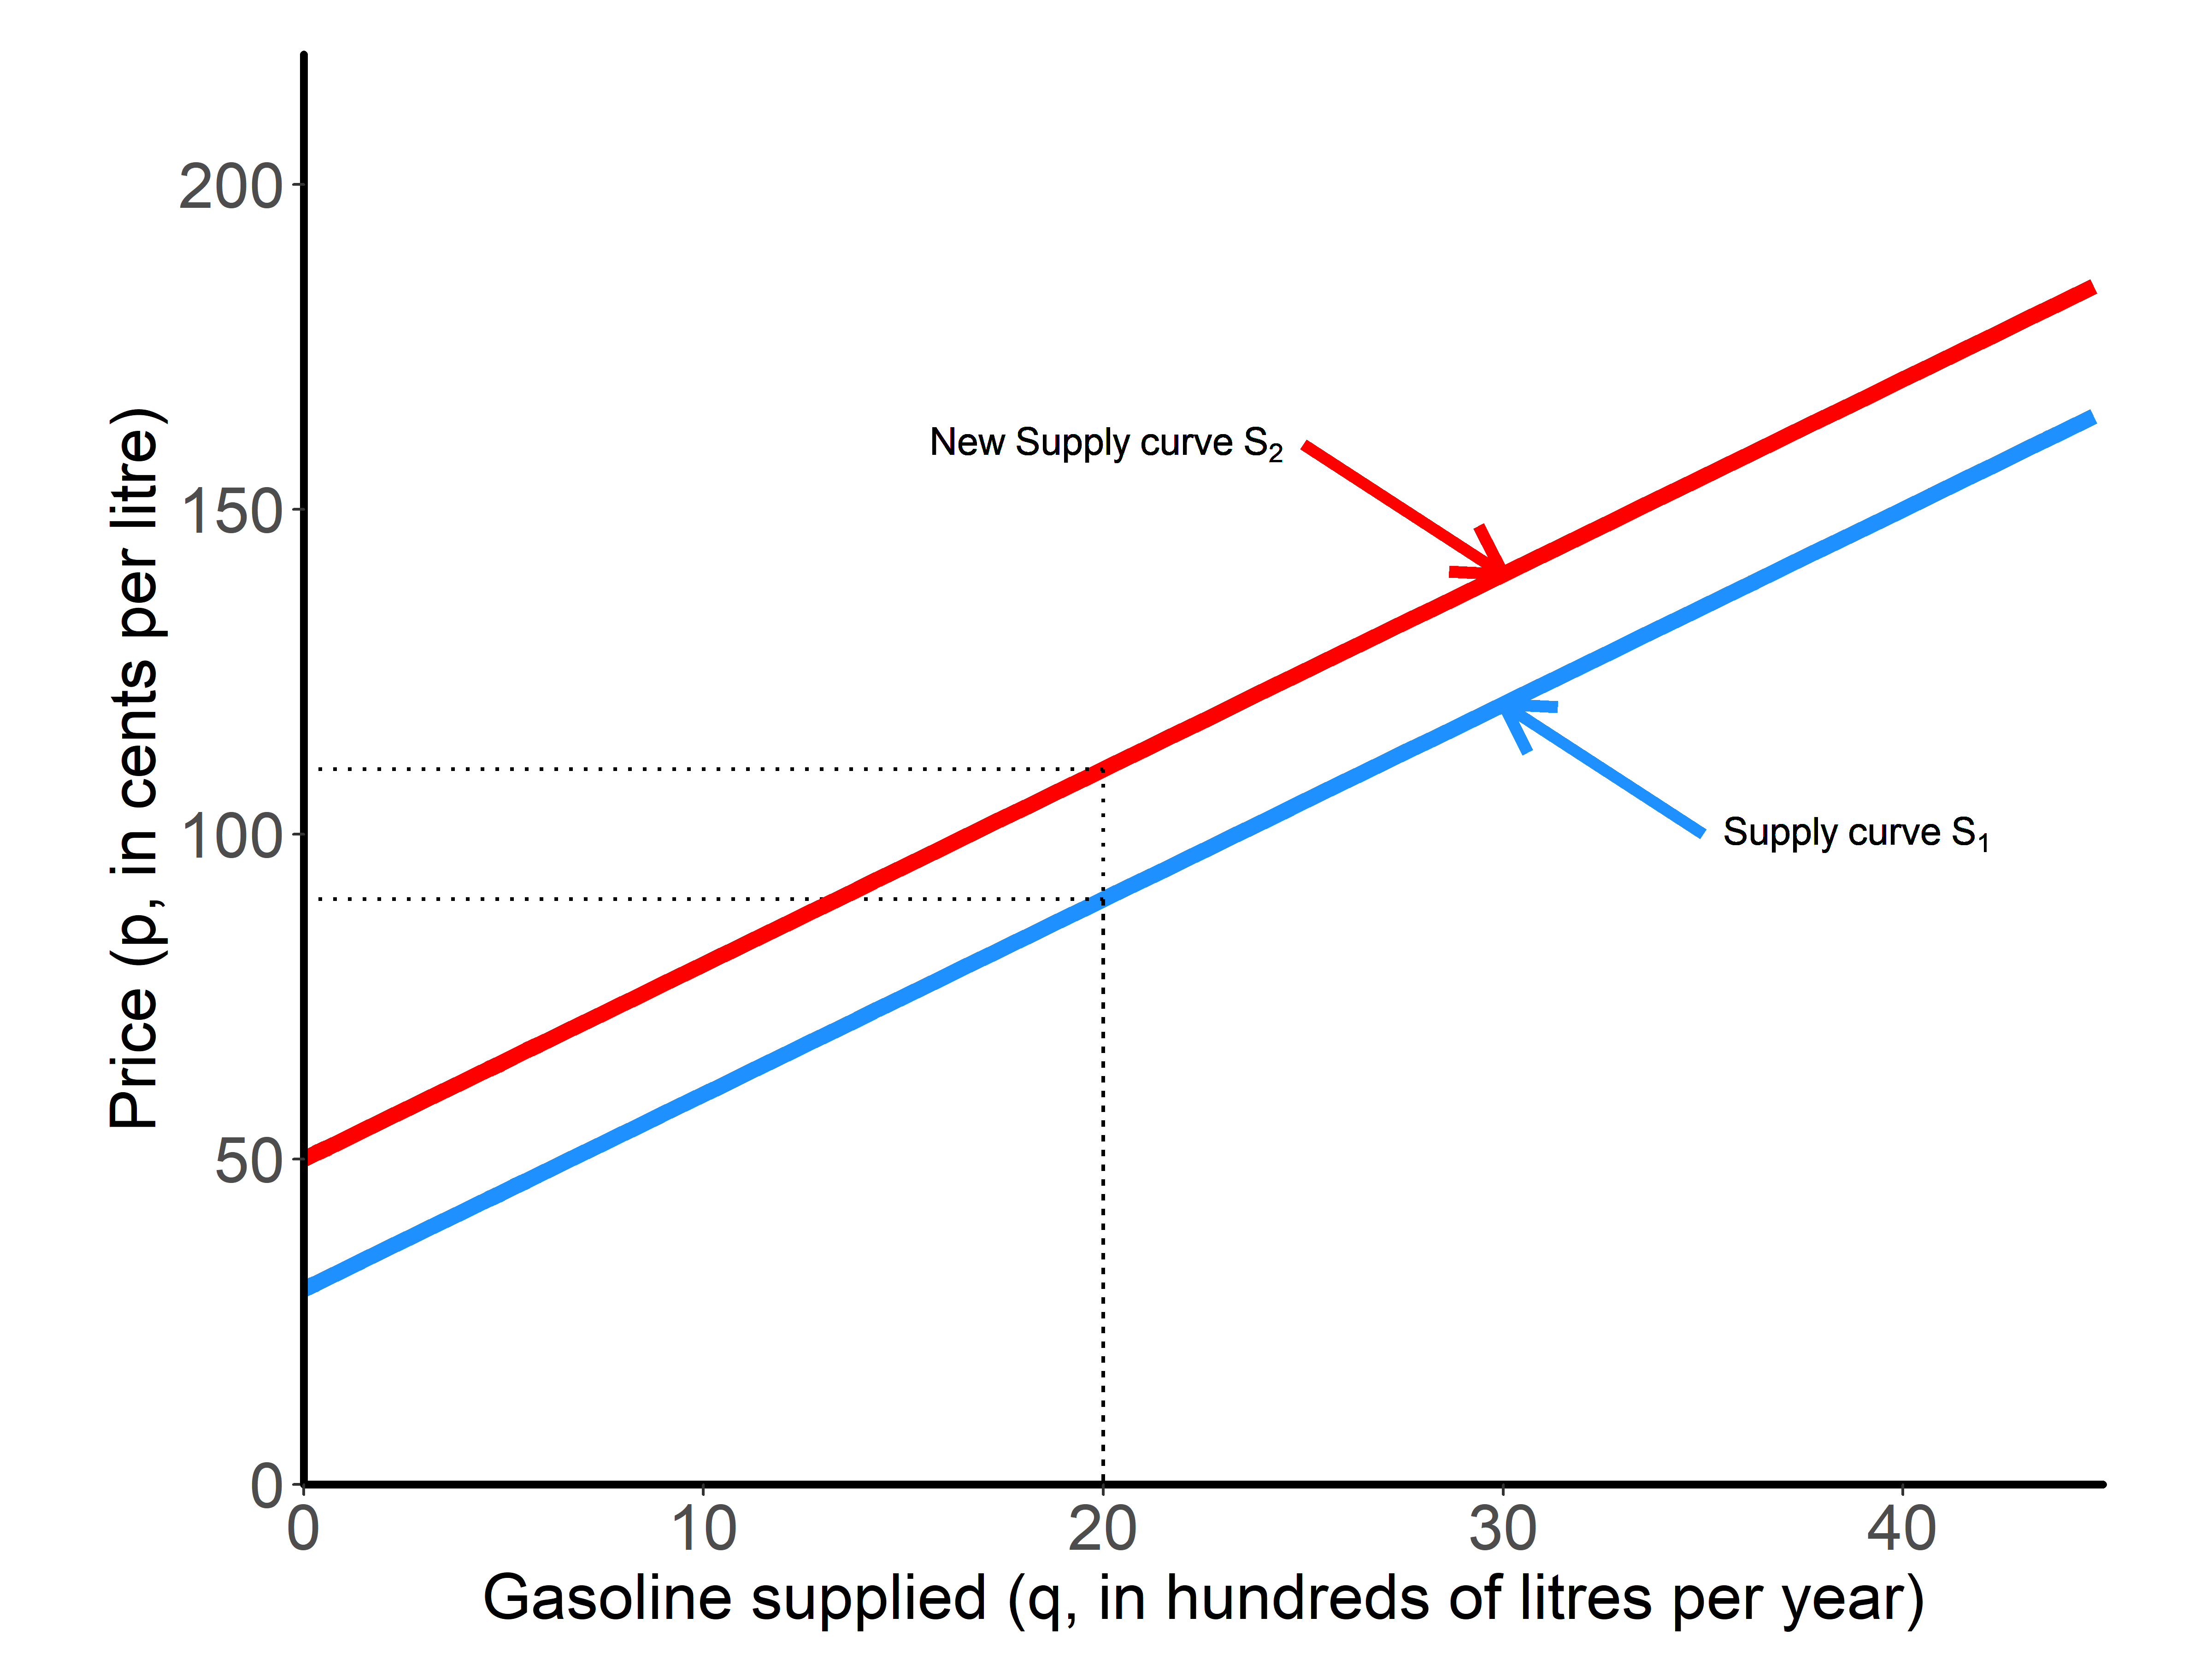
\includegraphics[width=\textwidth]{../images/gas_sup_shift.png}
}
\caption{The effect of a crude oil price increase on the supply of gasoline}
\end{figure}
}

\frame{
	\frametitle{The Supply Curve}
	\begin{itemize}
	\item How the supply curve shifts depends on the factor being considered.
		\begin{itemize}
		\item Prices.
		\item Production costs.
		\item Technological change.
		\item Government regulation.
		\end{itemize}
	\item[]
	\item As another example, let's consider the effects of a decrease in the price of blending components.
	\end{itemize}

}

\frame{
	\frametitle{The Supply Curve}
	%	The demand for gasoline:
\begin{figure}[t!]
	\center
	\resizebox{!}{.4\linewidth}{
    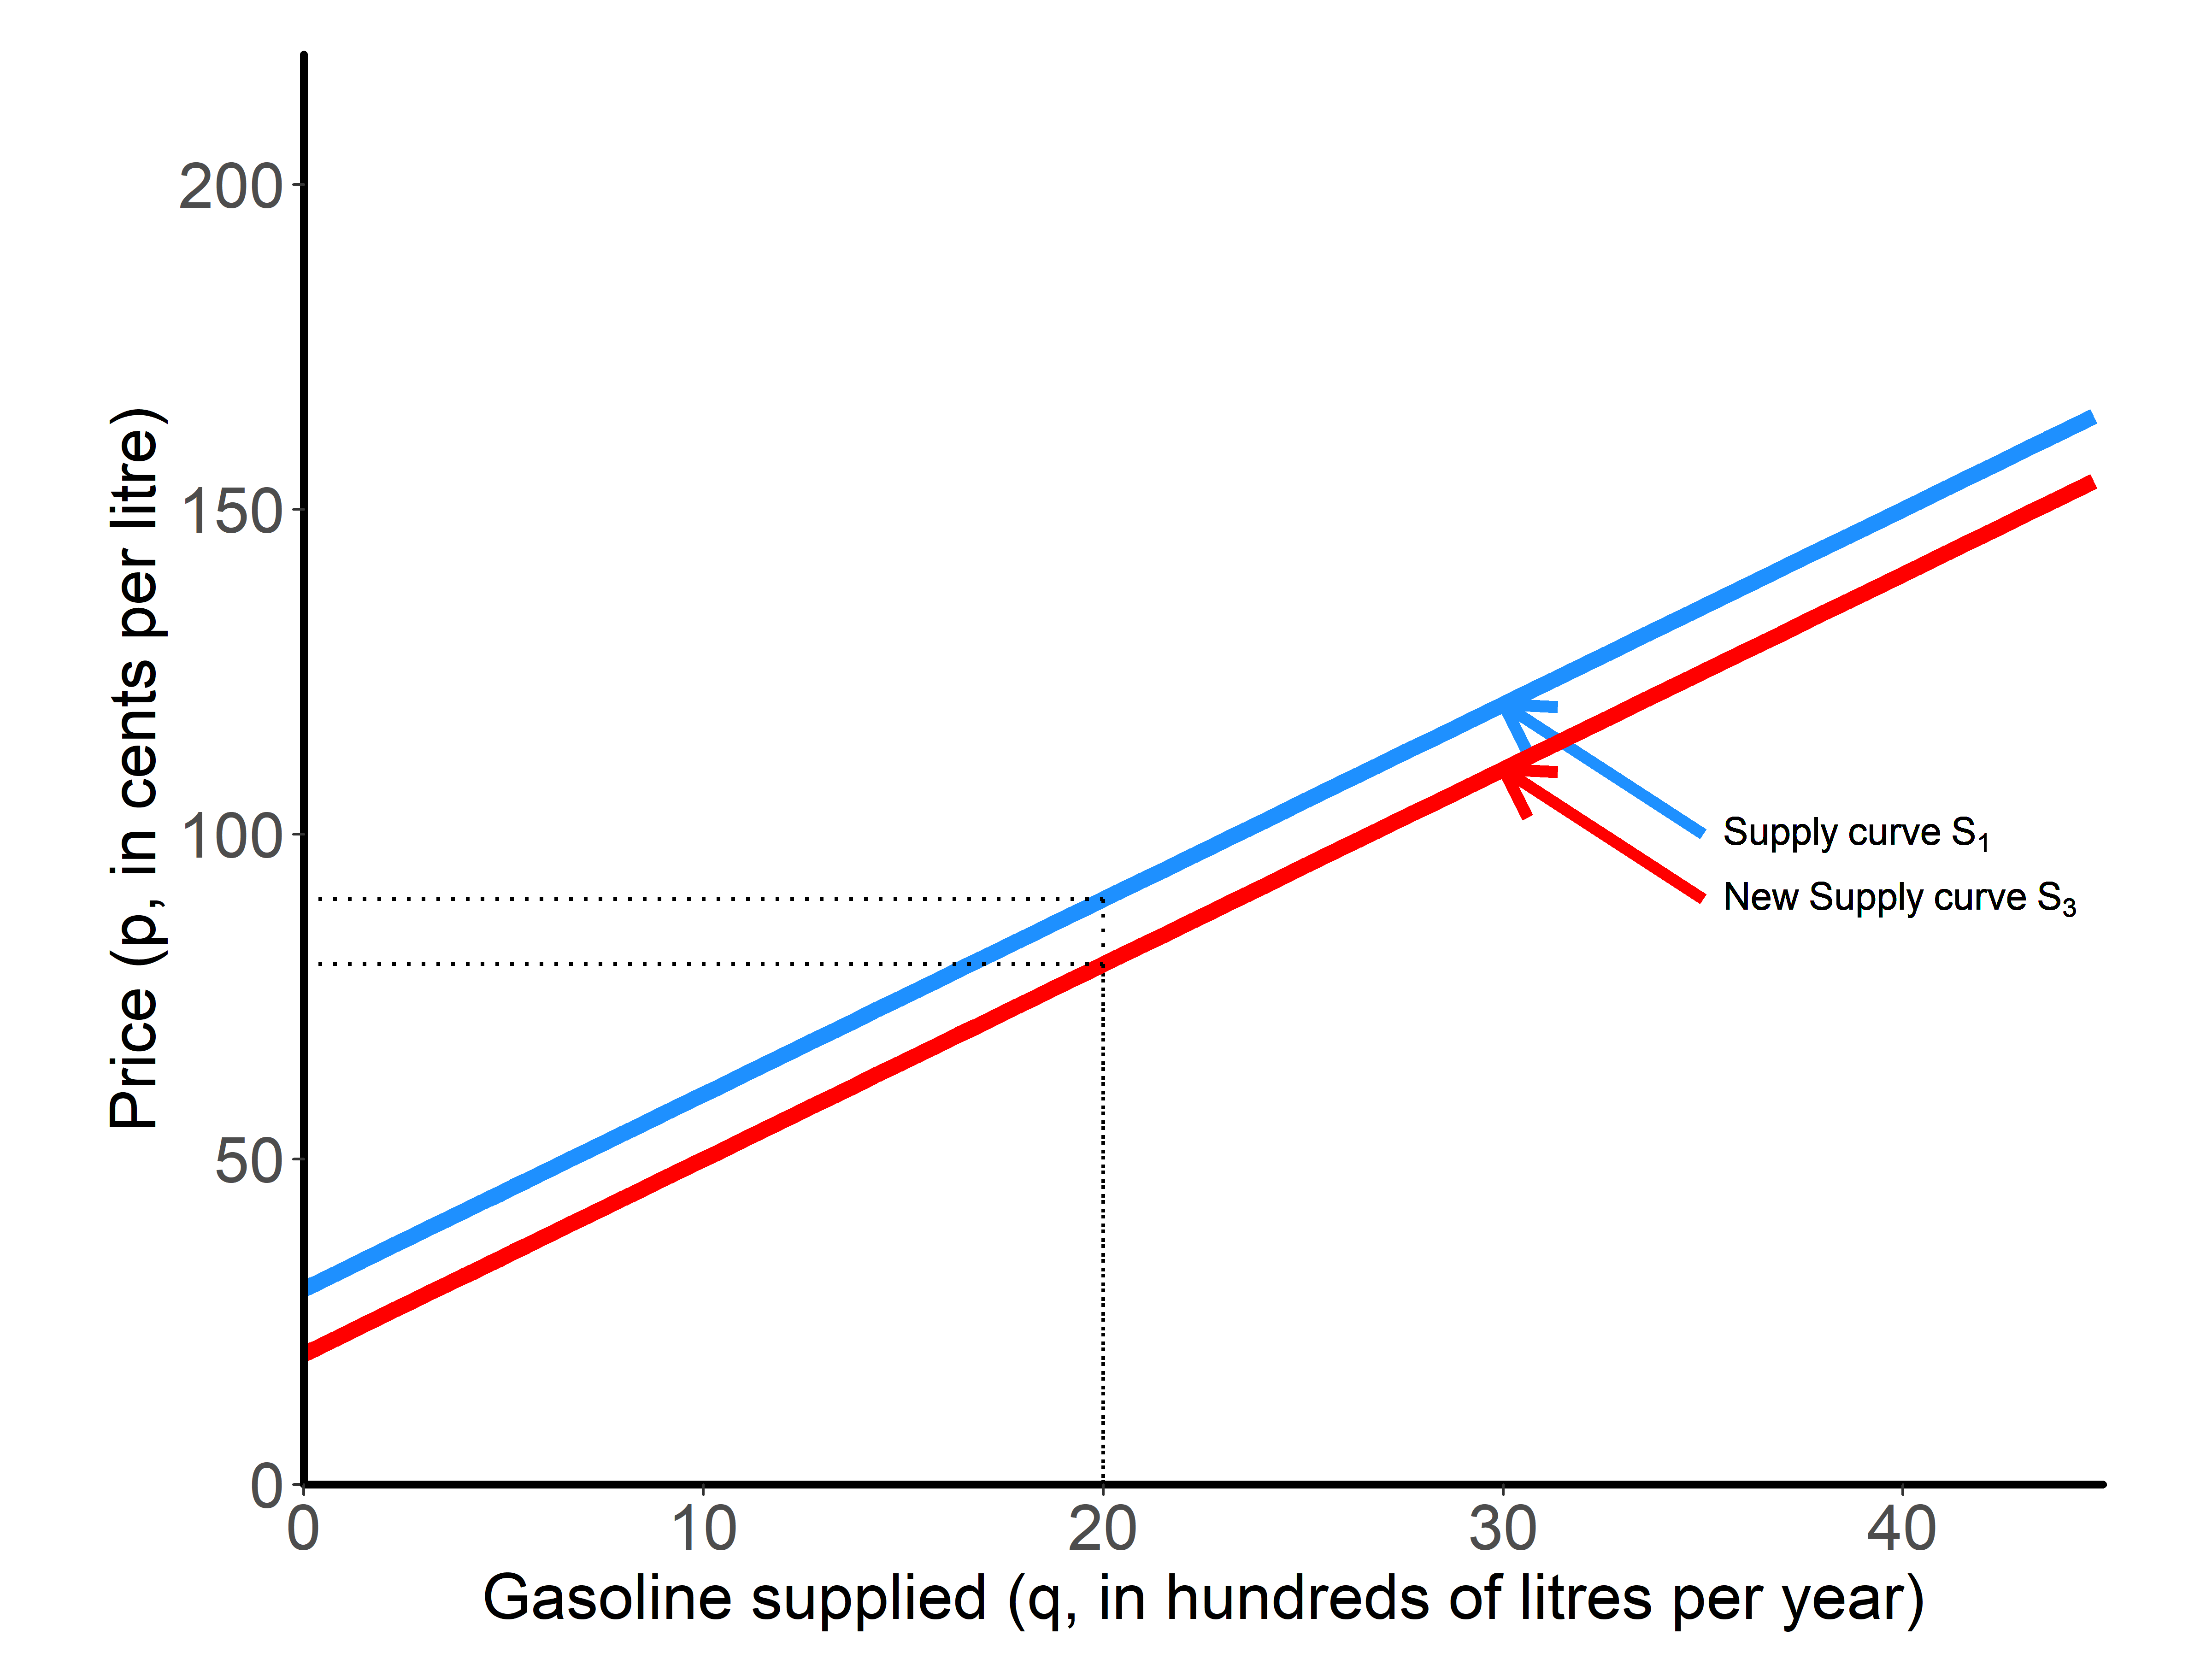
\includegraphics[width=\textwidth]{../images/gas_sup_shift_2.png}
}
\caption{The effect of a blending component cost decreases on the supply of gasoline}
\end{figure}
}

\frame{
	\frametitle{The Supply Curve}
	\begin{itemize}
	\item The supply curve displays the relationship between price and quantity supplied.
	\item We can also express this same relationship mathematically using a \textit{supply function}.
	\item The supply function is given by:
		\begin{align*}
		Q = S(p,p_{y},X)
		\end{align*}
		where $Q$ is the quantity supplied, and $S(-)$ is the supply function that depends on the
price, $p$, the price of other possible inputs or outputs $p_{y}$, and other factors, $X$.
		\item For simplicity, in what follows, we will hold other factors ($X$) constant.
	\end{itemize}
}

\frame{
	\frametitle{The Supply Function}
	\begin{itemize}
	\item Suppose that the estimated supply function for gasoline is given by:
		\begin{align*}
		Q =  10 + \frac{p}{3} - 0.5 p_{y}
		\end{align*}
		where $Q$ is the quantity of gasoline supplied, $p$ is the price of gasoline, and $p_{y}$ is the price of crude oil (these are just placeholder parameters).
		\begin{itemize}
		\item the own-price effect, $p$, is positive: higher p means higher Q.
		\item the impact of crude price changes, $p_{y}$ is negative: higher crude prices means less gasoline supplied at a given price.
		\item The constant term (10) reflects all other factors.
		\end{itemize}
	\end{itemize}
}

\frame{
	\frametitle{The Supply Function}
	\begin{itemize}
	\item We can obtain the supply curve by substituting for the price of crude oil, $p_{y}$.
	\item[]
	\item Suppose the price of oil is \$40 per barrel. Then the supply of gasoline is given by:
		\begin{align*}
		Q & = 10 + \frac{p}{3} - 0.5 p_{y}= 10 + \frac{p}{3} - 20\\
		 & = \frac{p}{3} - 10
		\end{align*}
	\item Rearranging we can obtain the \textit{inverse supply curve}, $p= 30+ 3Q$
	\item This is the same relationship depicted on the next slide.
	\end{itemize}
}

\frame{
	\frametitle{The Supply Function}
	%	The demand for gasoline:
	
		\begin{figure}[t!]
	\center
	\resizebox{!}{.4\linewidth}{
    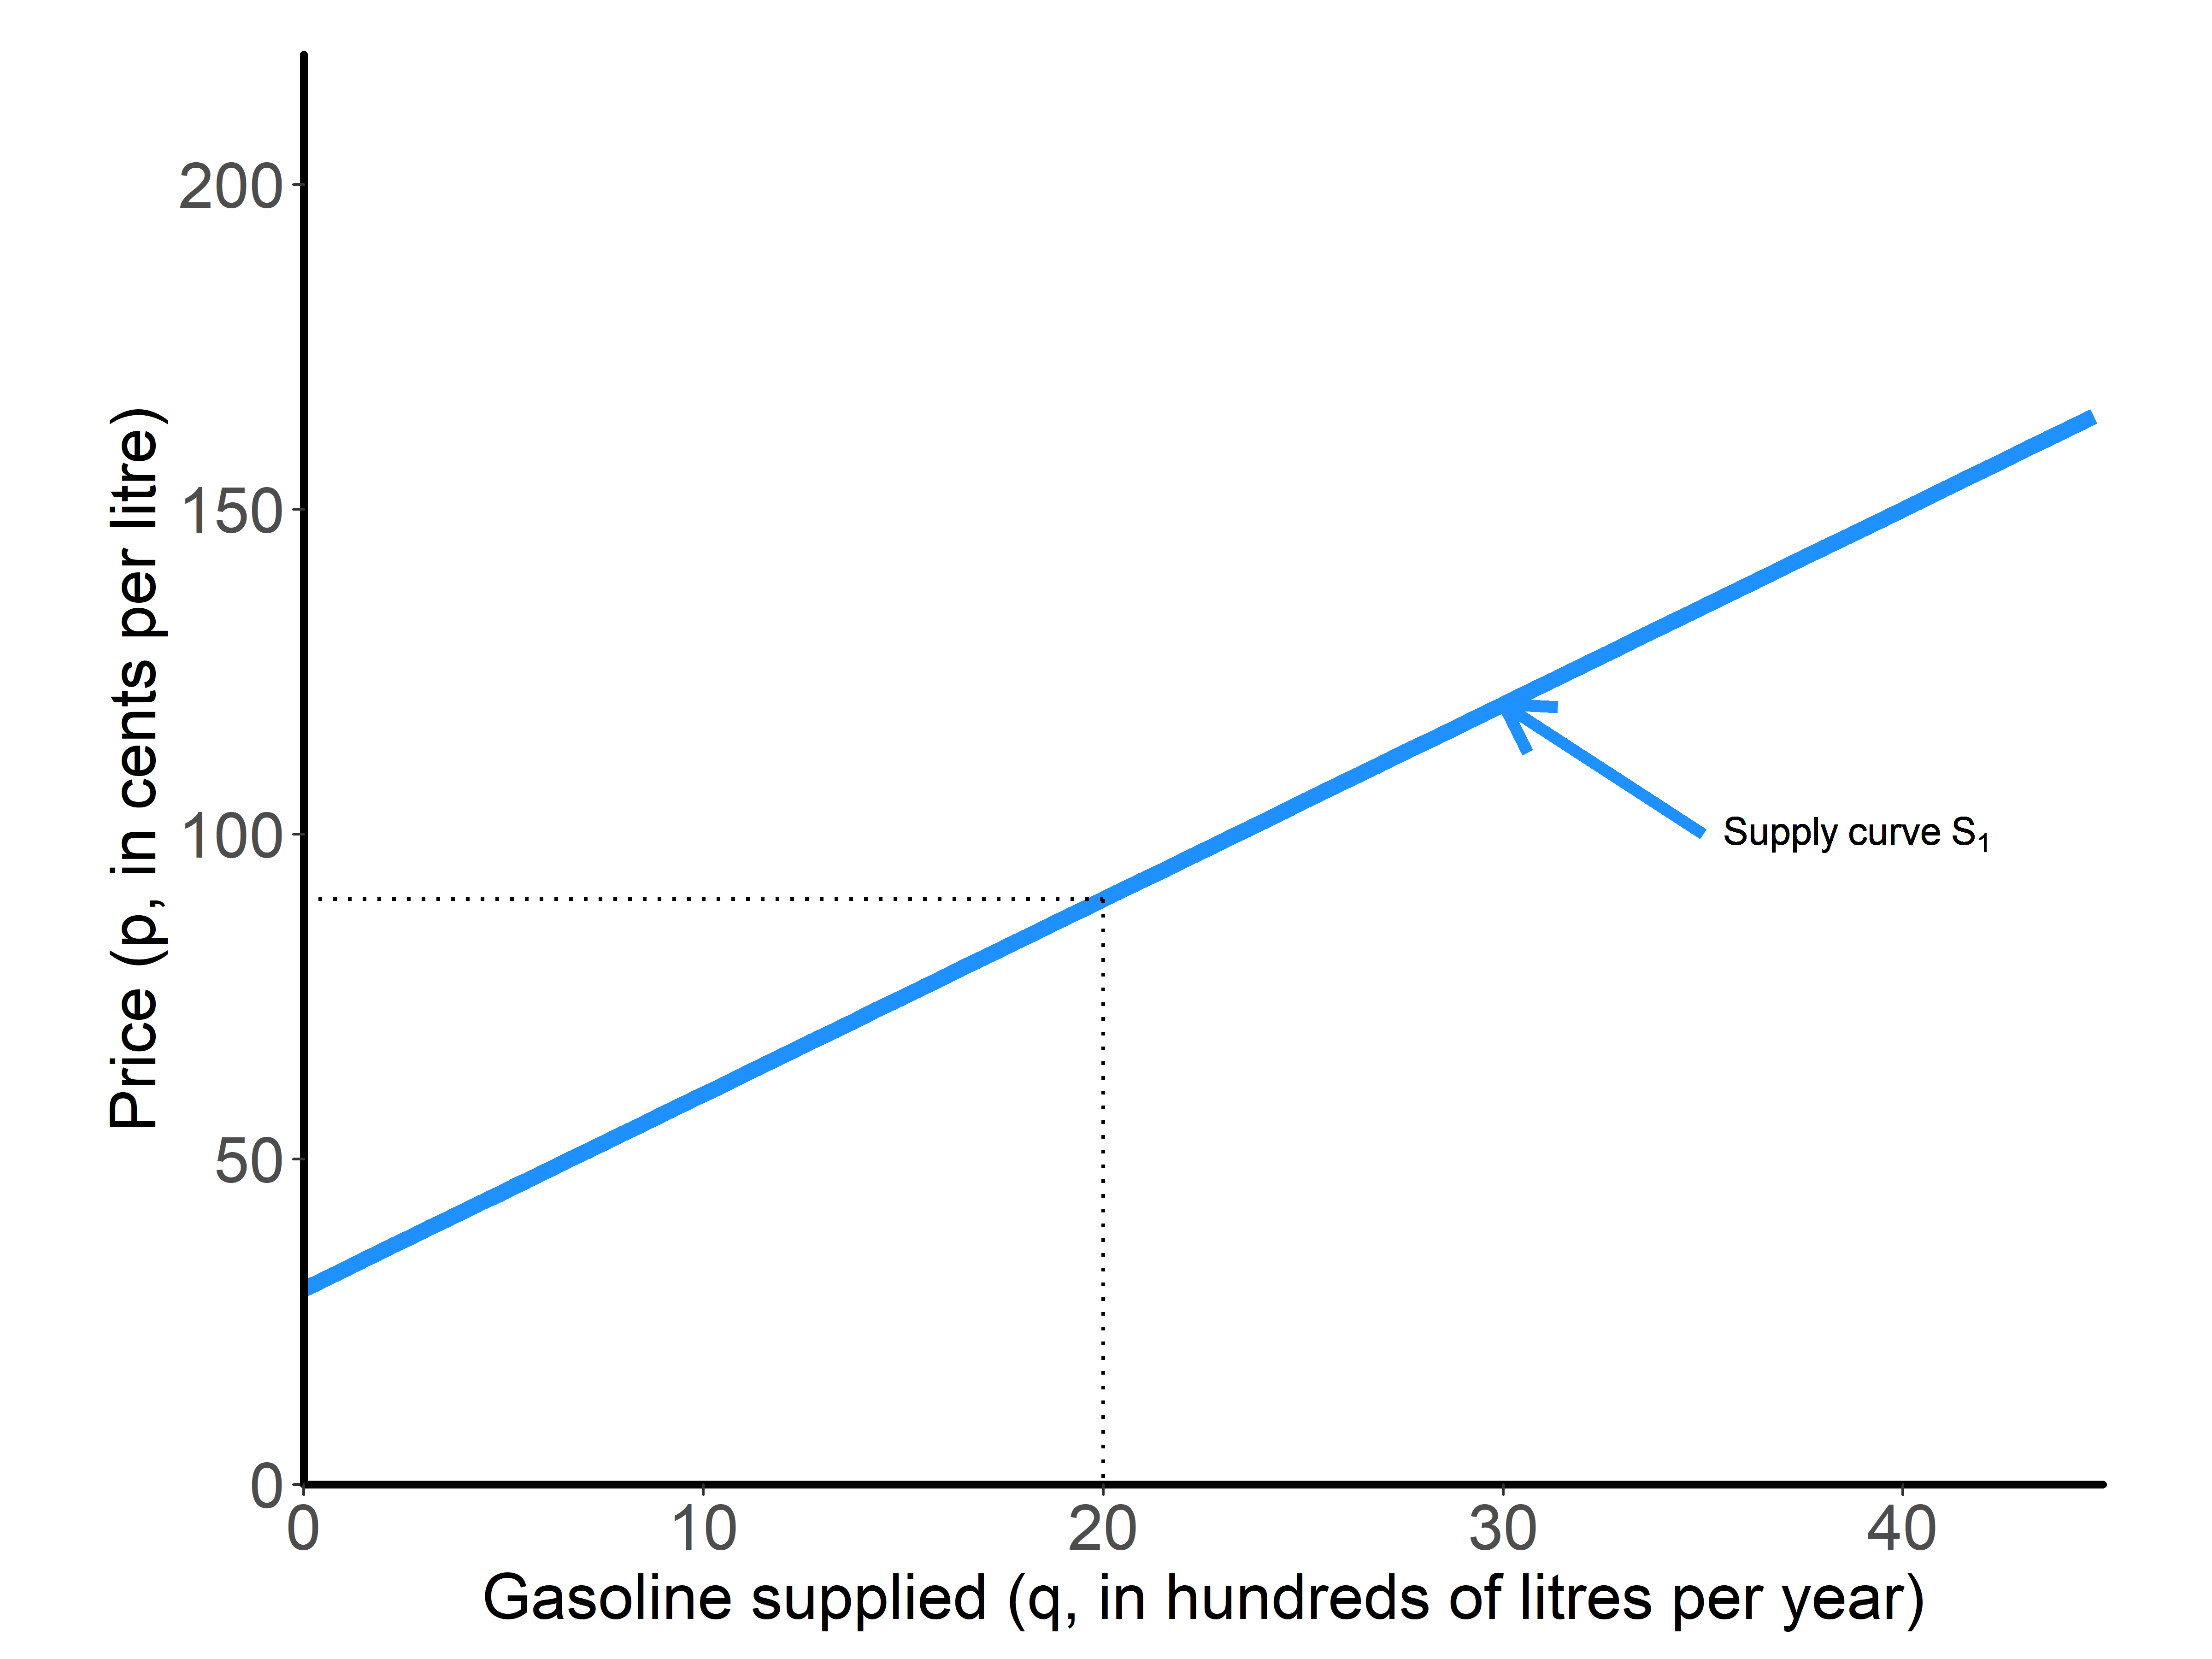
\includegraphics[width=\textwidth]{../images/gas_supply.png}
}
\caption{The supply of gasoline}
\end{figure}
}

\frame{
	\frametitle{The Supply Function}
	\begin{itemize}
	\item The supply function allows us to think precisely about how price changes affect the
quantity supplied, holding all other factors fixed.
    \item Let's use a simpler example here of $Q=2p$ and let $p_{1}$ denote the initial price, and $p_{2}$ denote the new price.
    \item The quantity supplied at $p_{1}$ is $Q_{1} = S(p_{1})=2p_1$, and the quantity supplied  at $p_{2}$ is $Q_{2} = S(p_{2})=2 p_2$
    \item The change in quantity supplied as price goes from $p_{1}$ to $p_{2}$ is $\Delta Q =
Q_{2}-Q_{1} = S(p_{2})-S(p_{1})$.
	
	\item In our simplified example, if the price changes from $p_{1}$ to $p_{2}$, the change in
quantity supplied is given by:
		\begin{align*}
		\Delta Q &= S(p_{2}) - S(p_{1}) = [2 p_{2}]- [2 p_{1}]\\
			& = 2 [p_{2}-p_{1}] = 2 \Delta p
		\end{align*}
	\end{itemize}
}

\frame{
	\frametitle{Determining Market Supply}
	\begin{itemize}
	\item In some cases, we may not have an estimate of total market supply, but rather estimates of
the supply curves of each producer in the market.
	\item[]
	\item To obtain total market supply, we need to add up the supply from each producer.
	\item[]
	\item Hint: Are you adding up prices or quantities?

	\end{itemize}
}	

\frame{
	\frametitle{Determining Market Supply}
	\begin{itemize}
	\item As an example, suppose there are 3 producers in the market for gasoline. They both have
supply functions given by:
		\begin{align*}
		Q = 2p
		\end{align*}
		what is the market supply of gasoline in this case?
	\end{itemize}
}



\frame{
	\frametitle{Determining Market Supply}
	%	The demand for gasoline:
\begin{figure}[t!]
	\center
	\resizebox{!}{.4\linewidth}{
    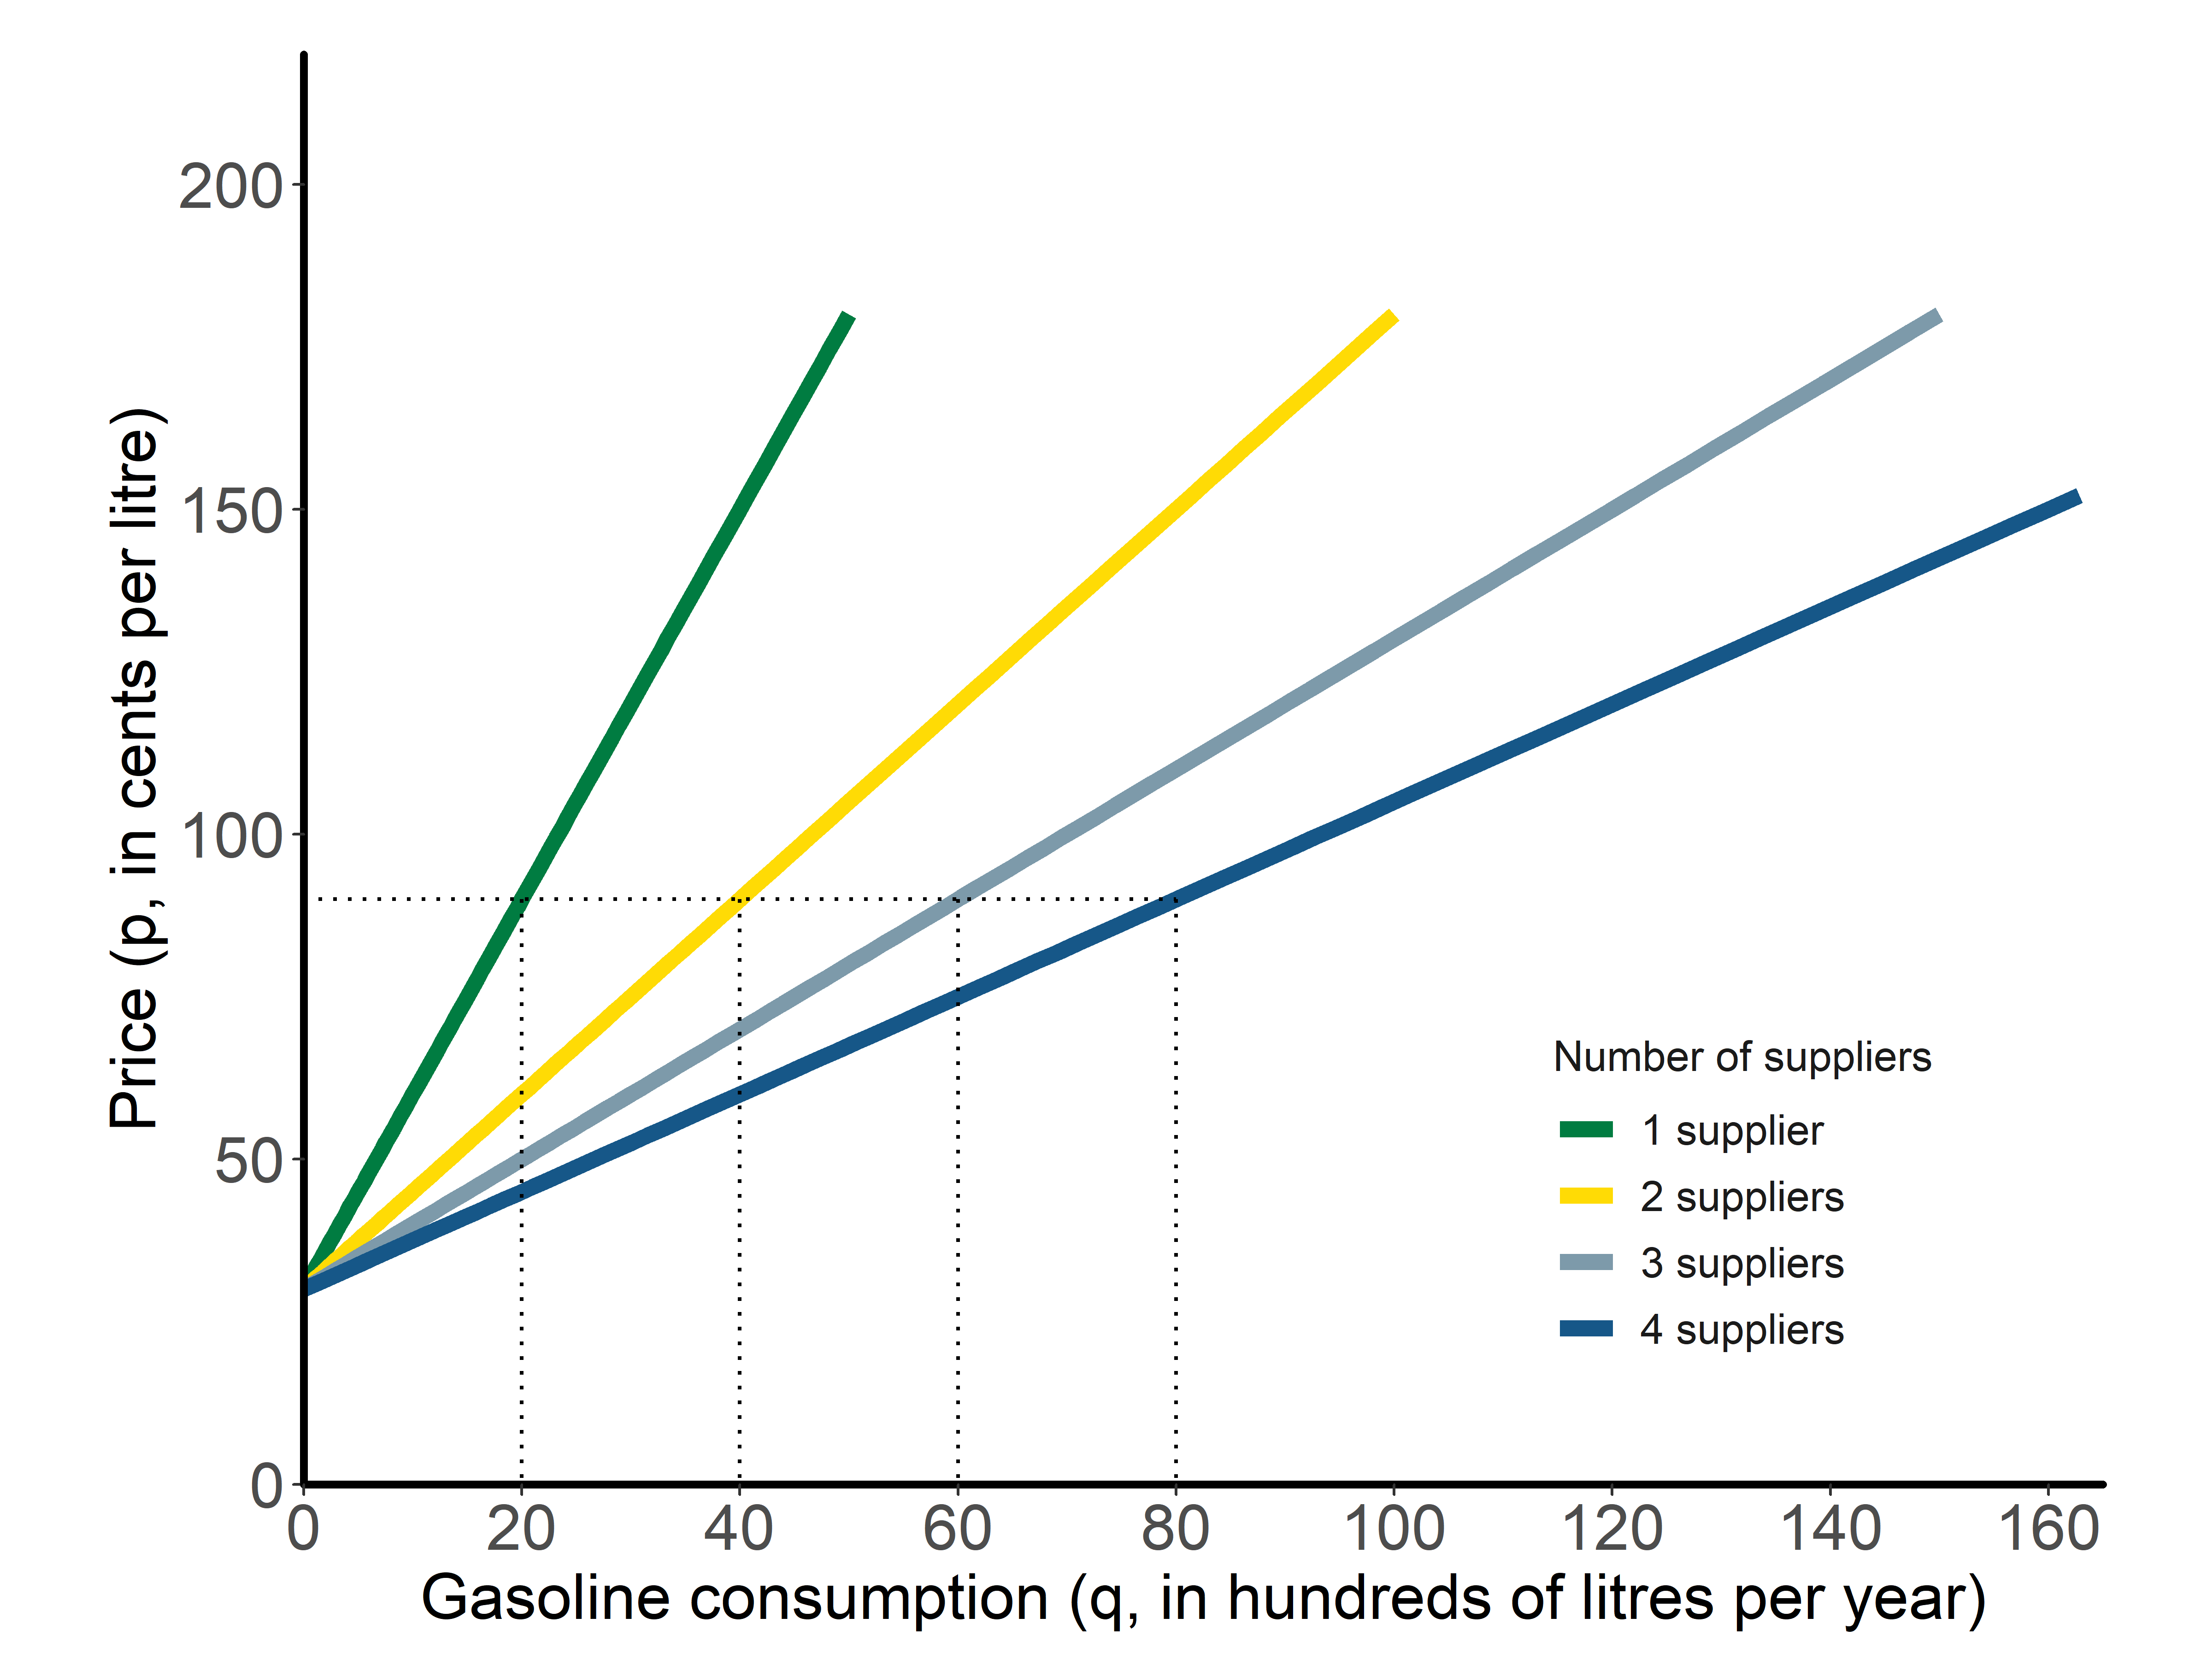
\includegraphics[width=\textwidth]{../images/gas_sup_stack.png}
}
\caption{The aggregate supply of gasoline using the same equations as above}
\end{figure}
}


\section{Equilibrium}

\frame{
	\frametitle{Market Equilibrium}
	\begin{itemize}
	\item Once we know supply and demand in the market, we can determine the \textit{market
equilibrium}.
	\end{itemize}
	\begin{definition}[Market Equilibrium]
	The market is in equilibrium when all market participants are able to buy or sell as much as they
want; no participant wants to change their behaviour given what other market participants are doing.
	\end{definition}
}

\frame{
	\frametitle{Market Equilibrium}
	\begin{itemize}
	\item How can we determine the market equilibrium from the supply and demand curves?
	\end{itemize}
}

\frame{
	\frametitle{Market Equilibrium}
	
		\begin{figure}[t!]
    \center
	\resizebox{!}{.4\linewidth}{
    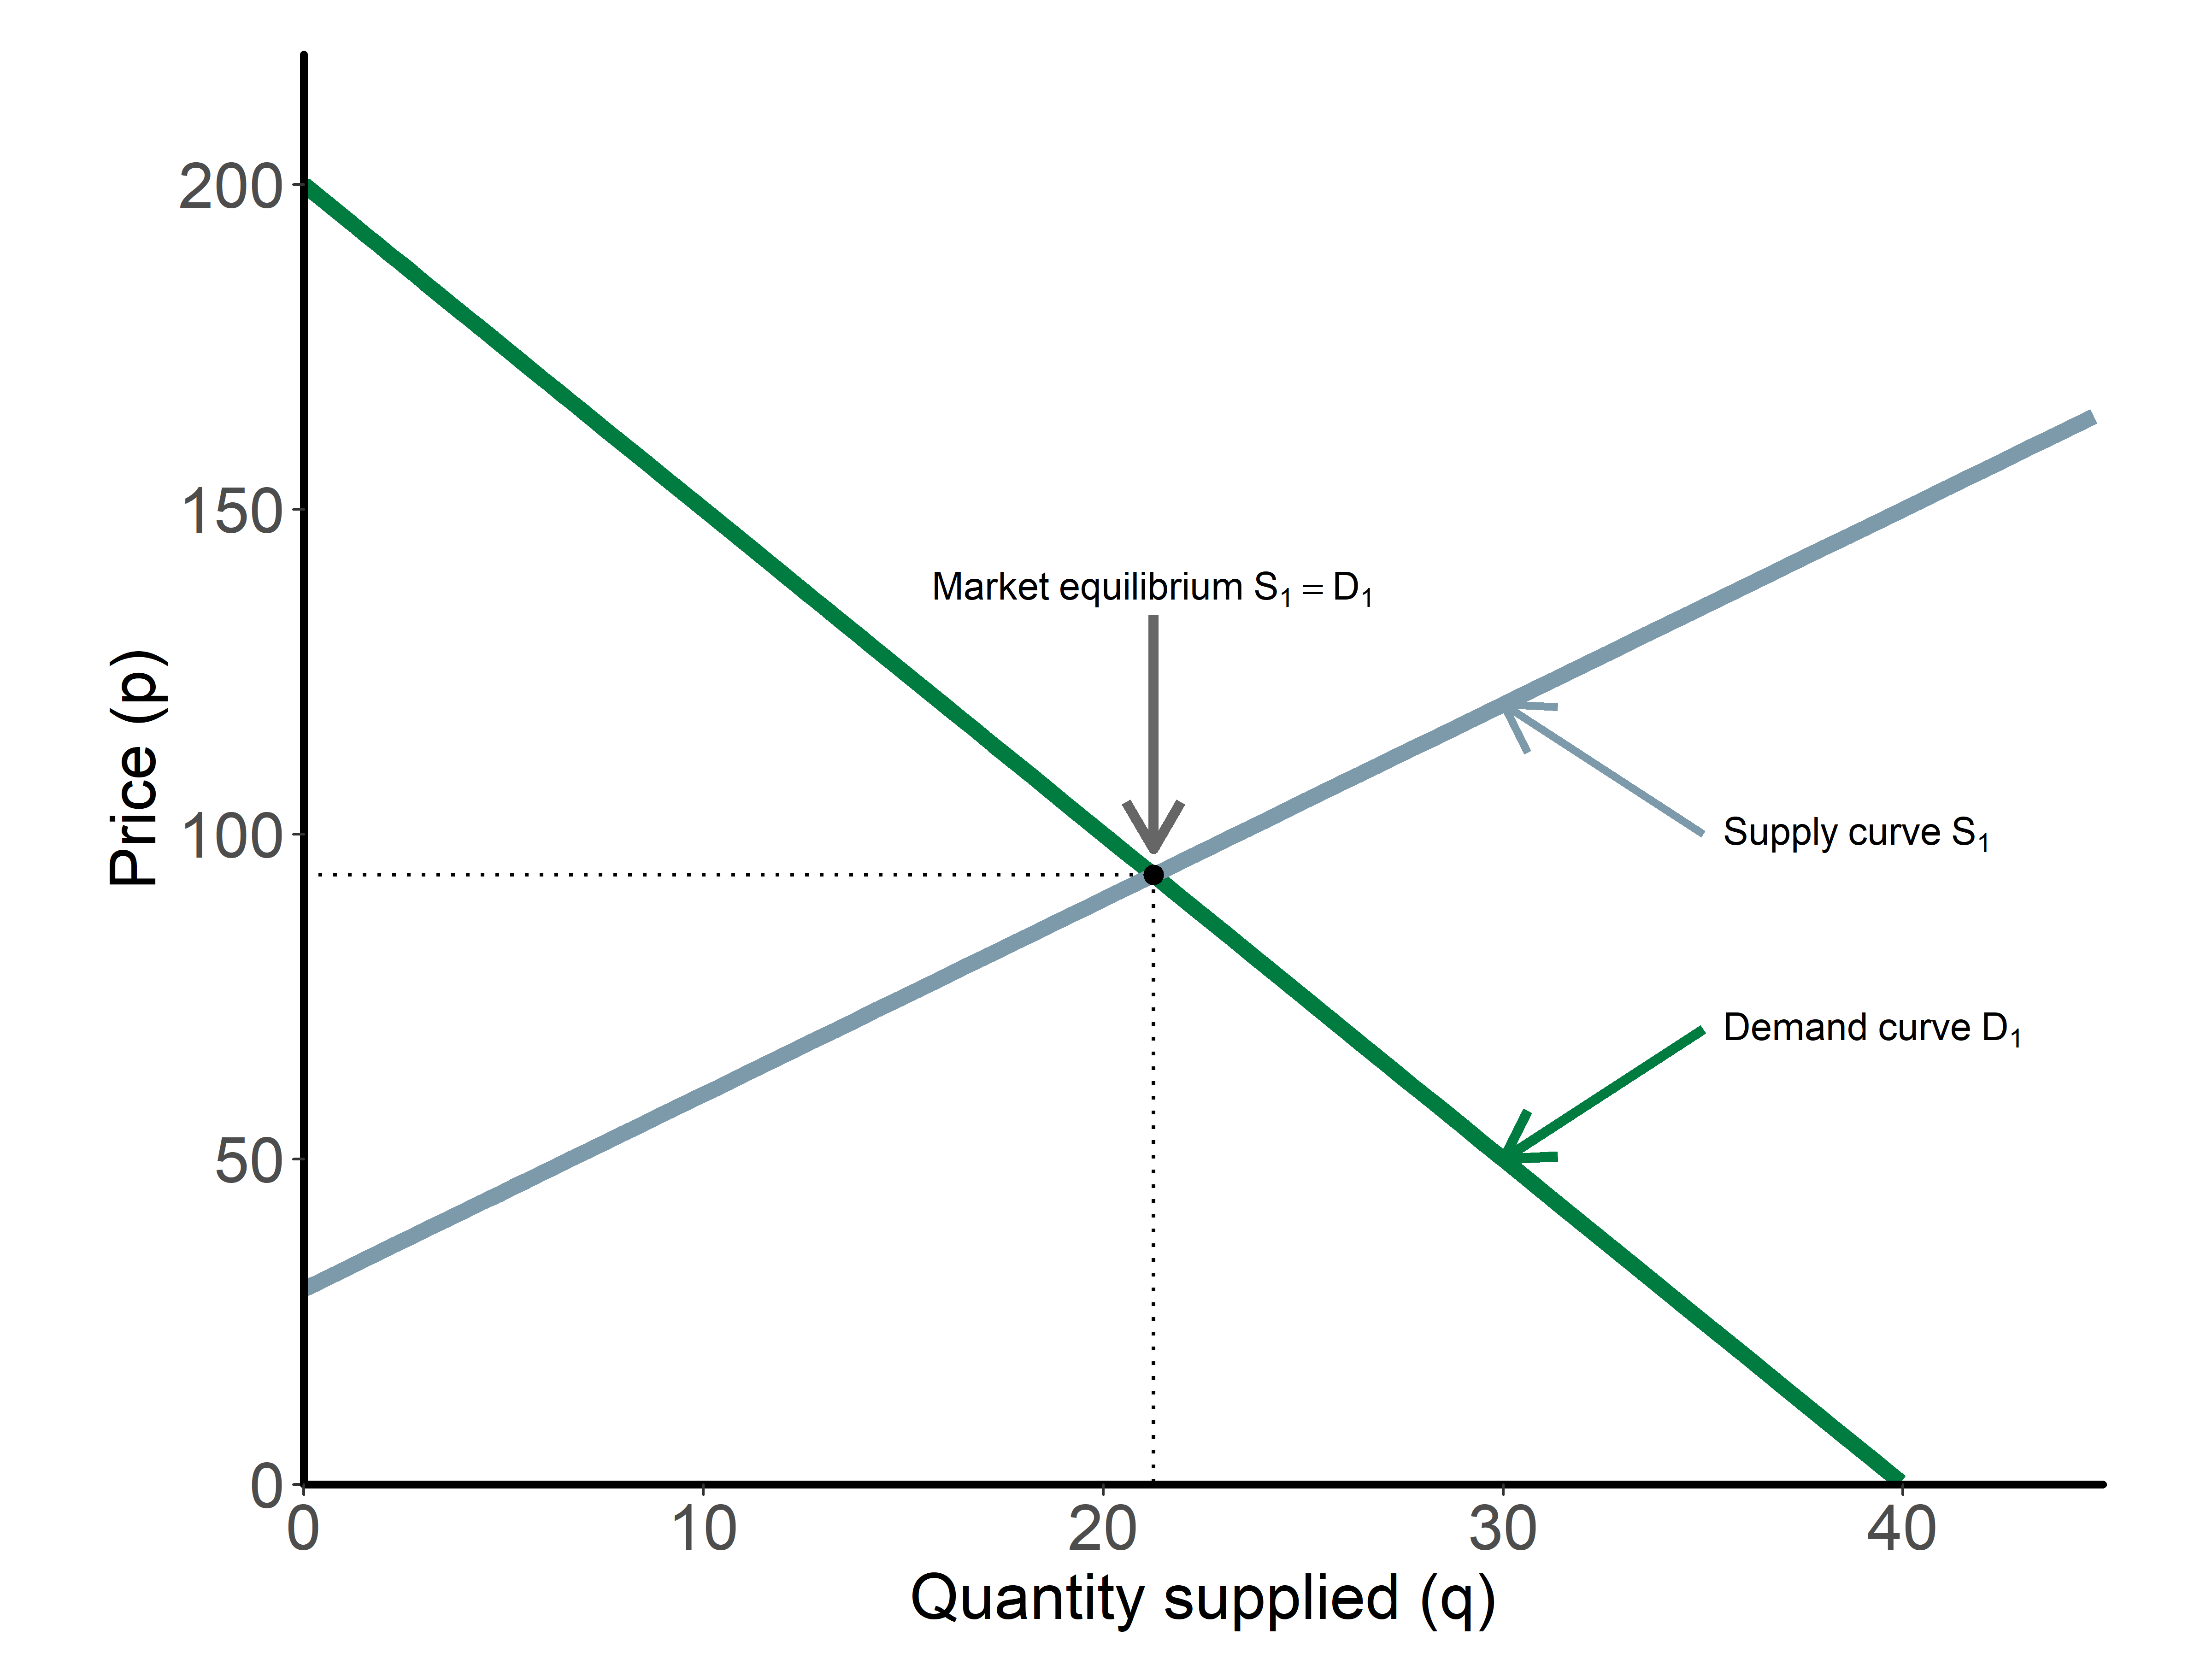
\includegraphics[width=\textwidth]{../images/basic_equil.png}
}
	
\caption{Equilibrium in the market}
\end{figure}
}


\frame{
	\frametitle{Market Equilibrium}
	\begin{definition}[Equilibrium Price]
	The equilibrium price is the $p$ at which consumers can buy as much as they want, and sellers can
sell as much as they want.
	\end{definition}
	
	\begin{definition}[Equilibrium Quantity]
	The equilibrium quantity is the $q$ such that the quantity demanded equals the quantity supplied.
	\end{definition}
}

\frame{
	\frametitle{Market Equilibrium}
	
		\begin{figure}[t!]
    \center
	\resizebox{!}{.4\linewidth}{
    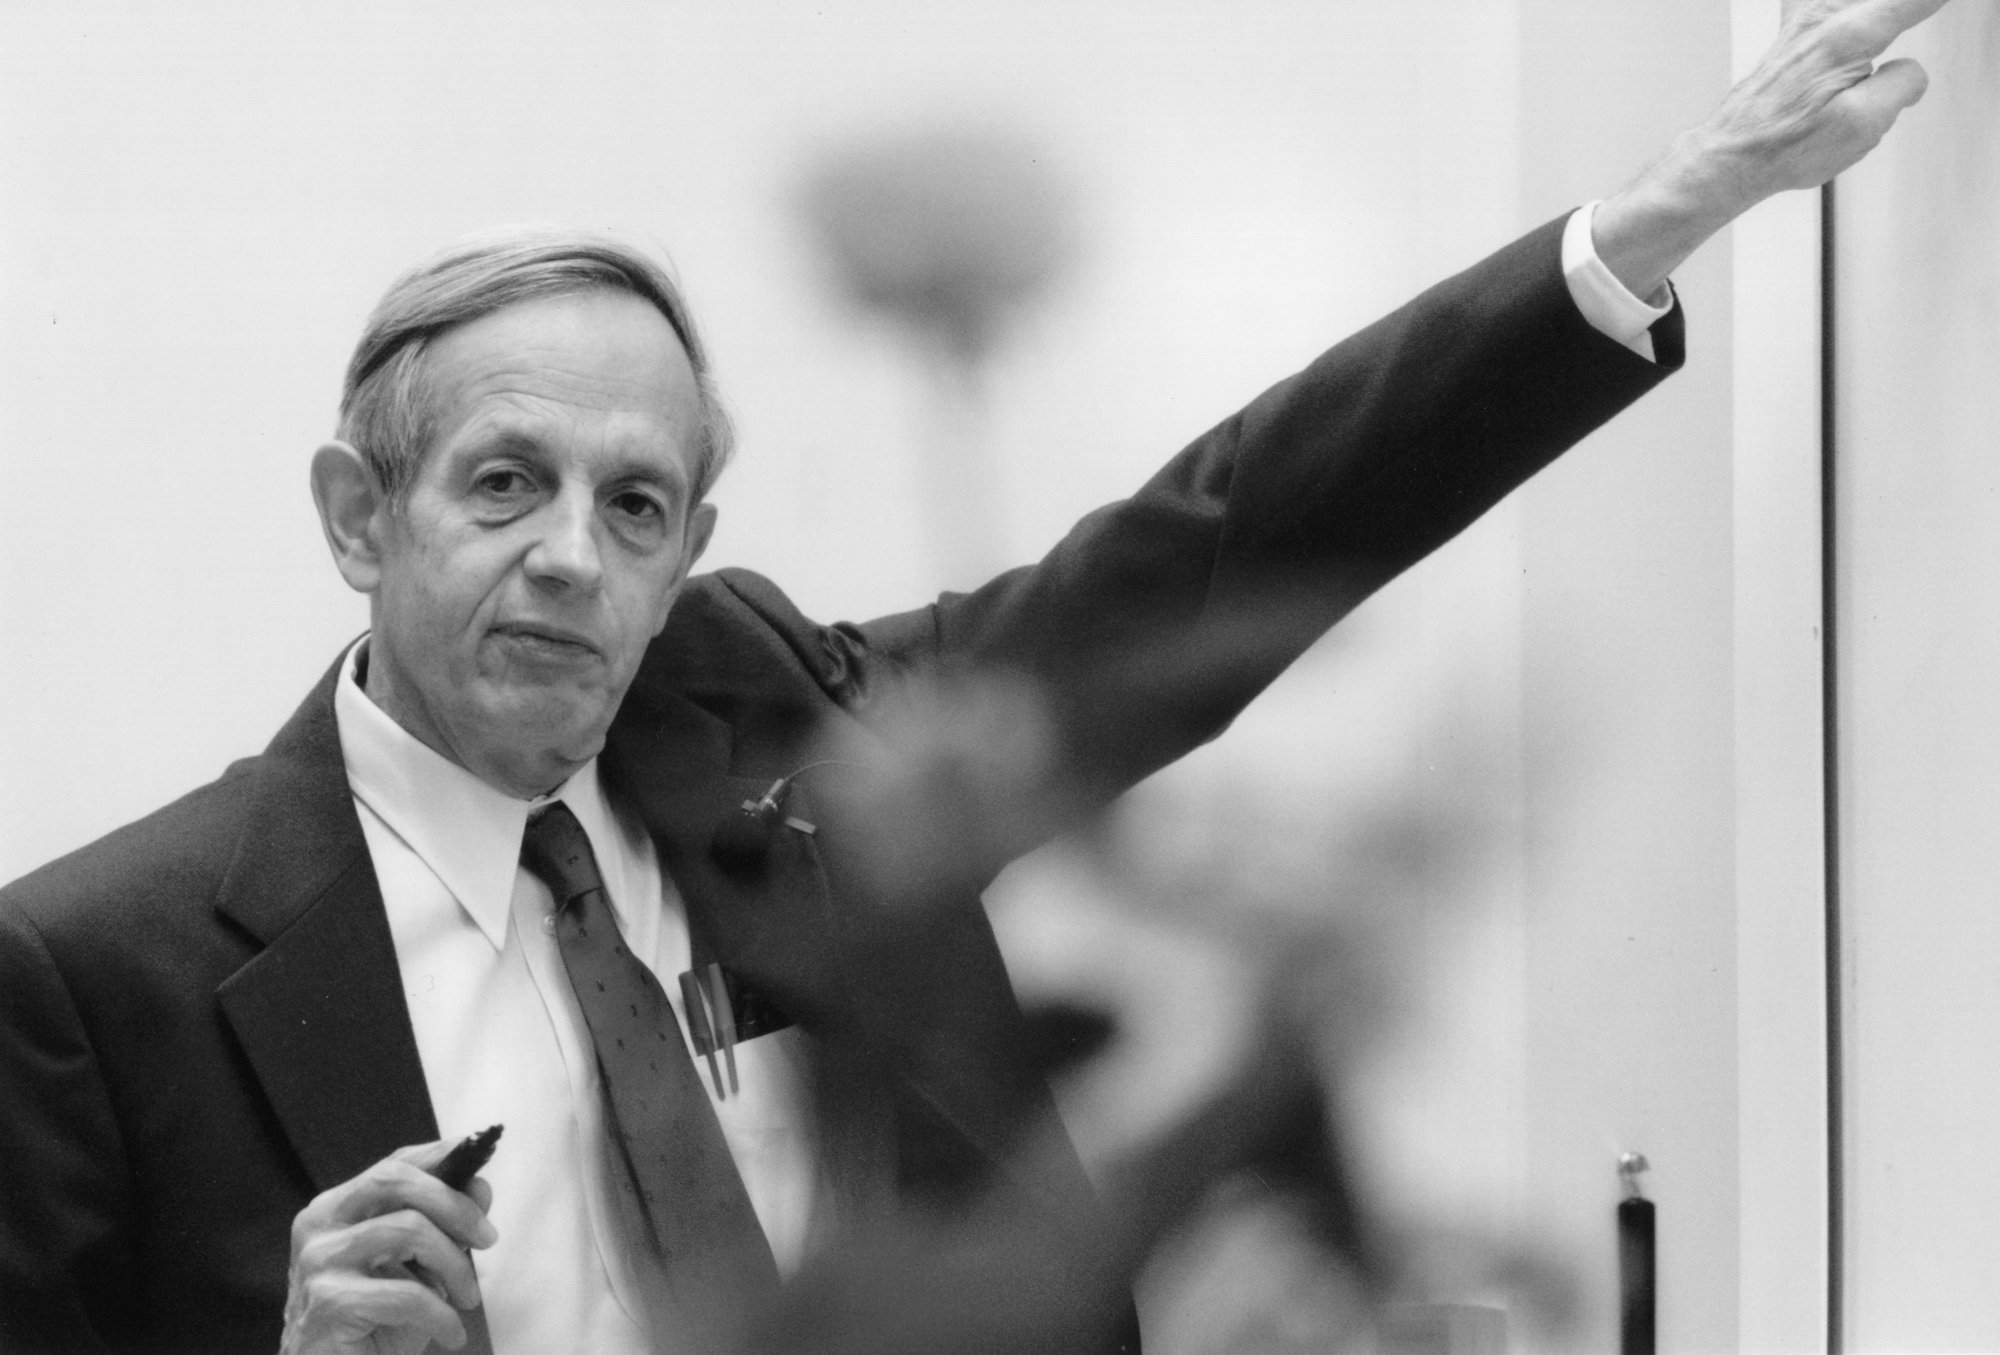
\includegraphics[width=\textwidth]{../images/nash.jpg}
}
	\caption{Our modern understanding of equilibrium in the market is largely due to this economist. Image: PBS}
\end{figure}
}

\frame{
	\frametitle{Market Equilibrium}
	
		\begin{figure}[t!]
    \center
	\resizebox{!}{.4\linewidth}{
    
\includegraphics[width=\textwidth]{../images/nash_2.jpg}
}
	\caption{They even made a movie about him: A Beautiful Mind (2001)}
\end{figure}
}


\frame{
	\frametitle{Market Equilibrium}
	
		\begin{figure}[t!]
    \center
	\resizebox{!}{.4\linewidth}{
    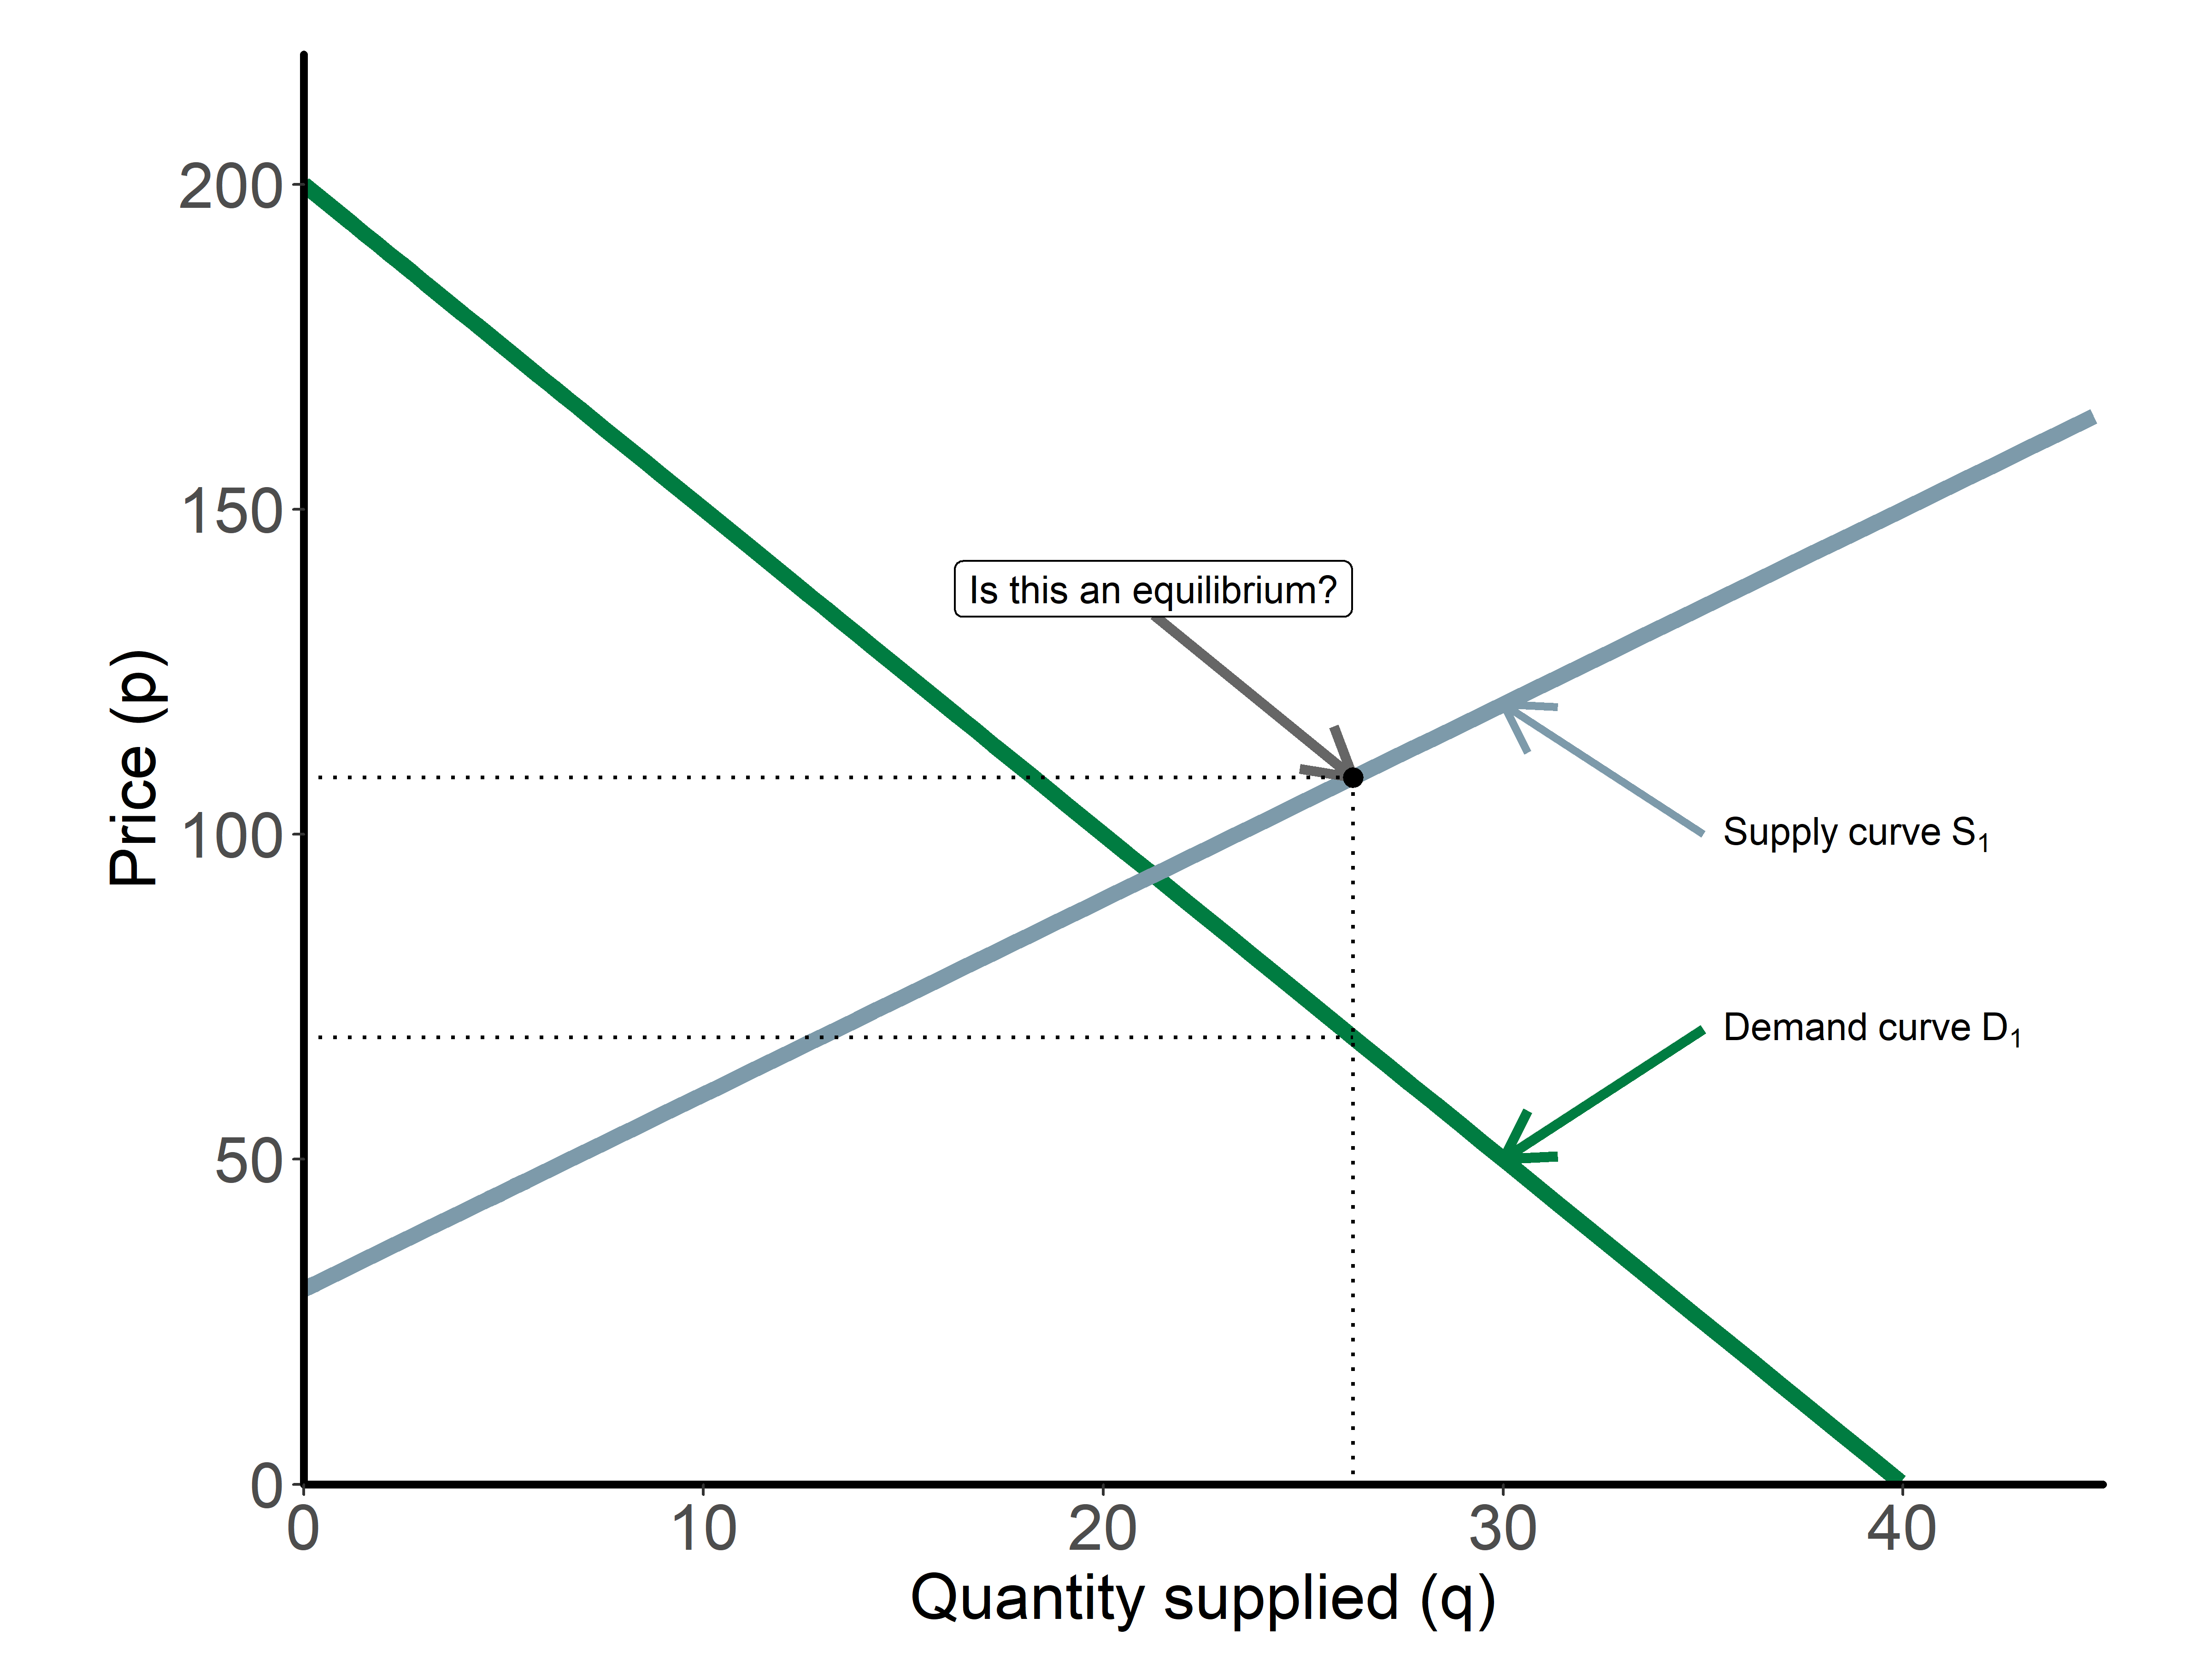
\includegraphics[width=\textwidth]{../images/equil_expl_1.png}
}
\caption{Off-equilibrium points, and the rationale of equilibrium}
\end{figure}
}
	

\frame{
	\frametitle{Market Equilibrium}
	
		\begin{figure}[t!]
    \center
	\resizebox{!}{.4\linewidth}{
    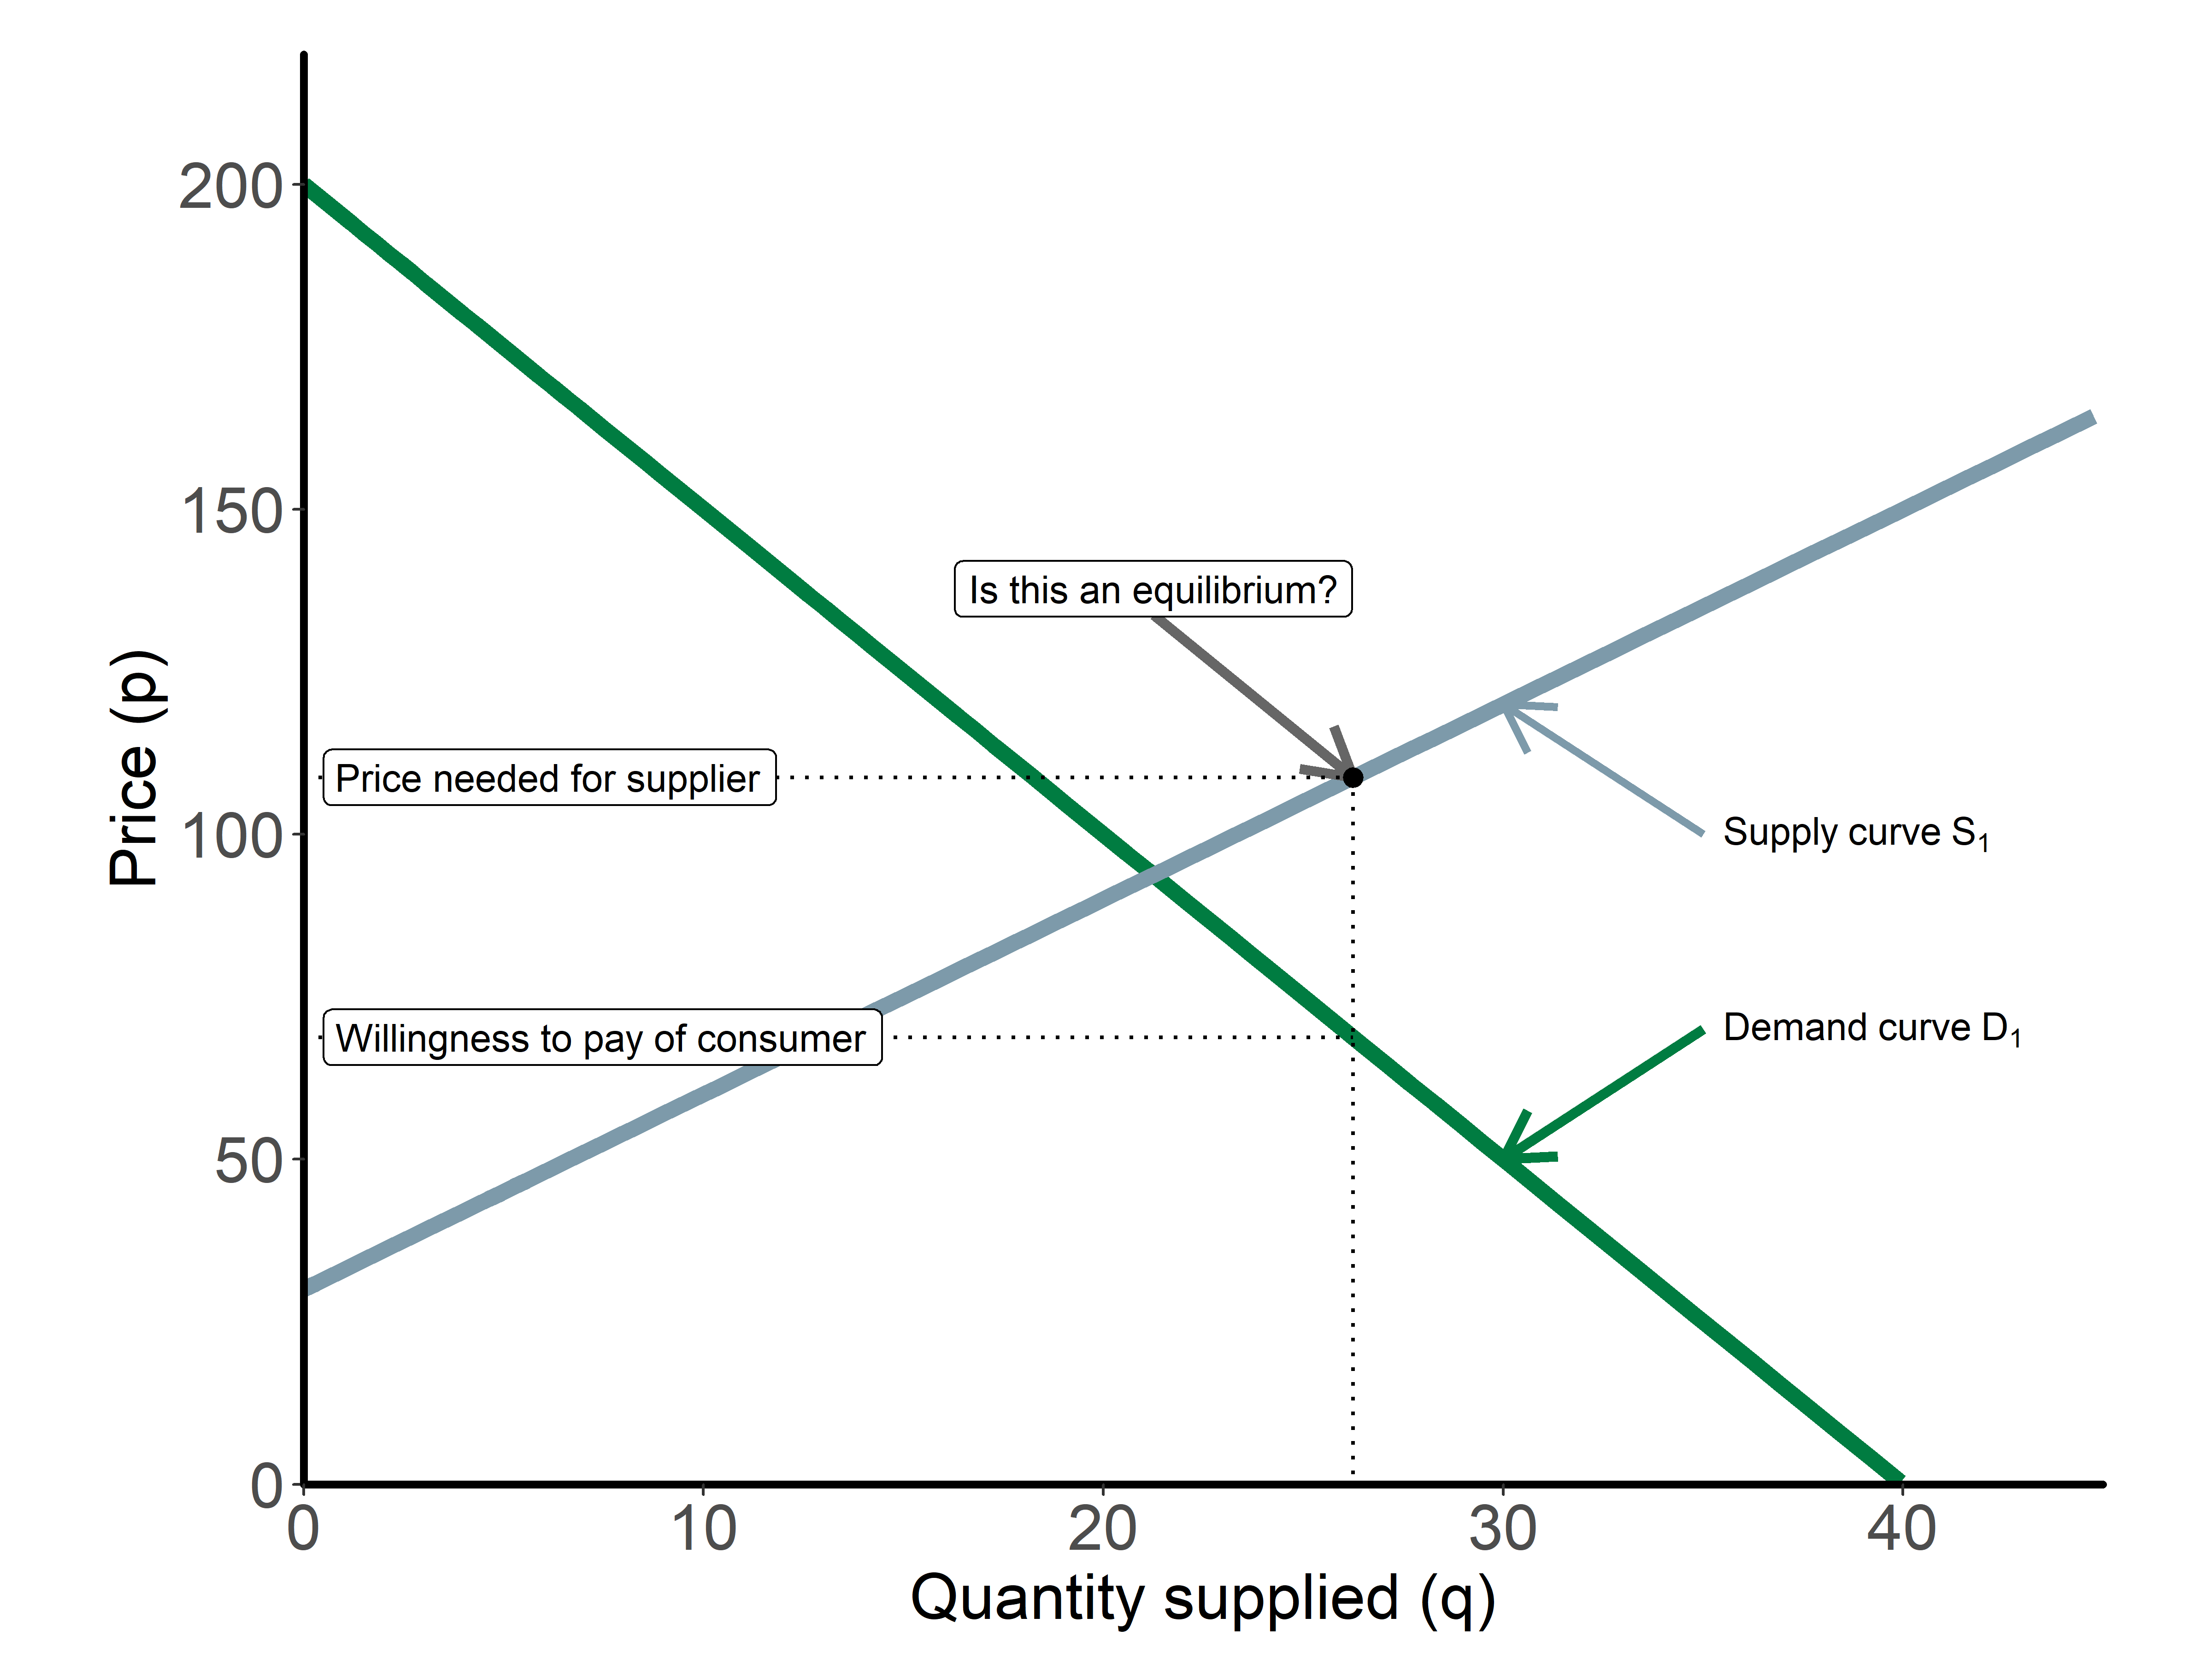
\includegraphics[width=\textwidth]{../images/equil_expl_2.png}
}
\caption{Off-equilibrium points, and the rationale of equilibrium}
\end{figure}
}

\frame{
	\frametitle{Market Equilibrium}
	
		\begin{figure}[t!]
    \center
	\resizebox{!}{.4\linewidth}{
    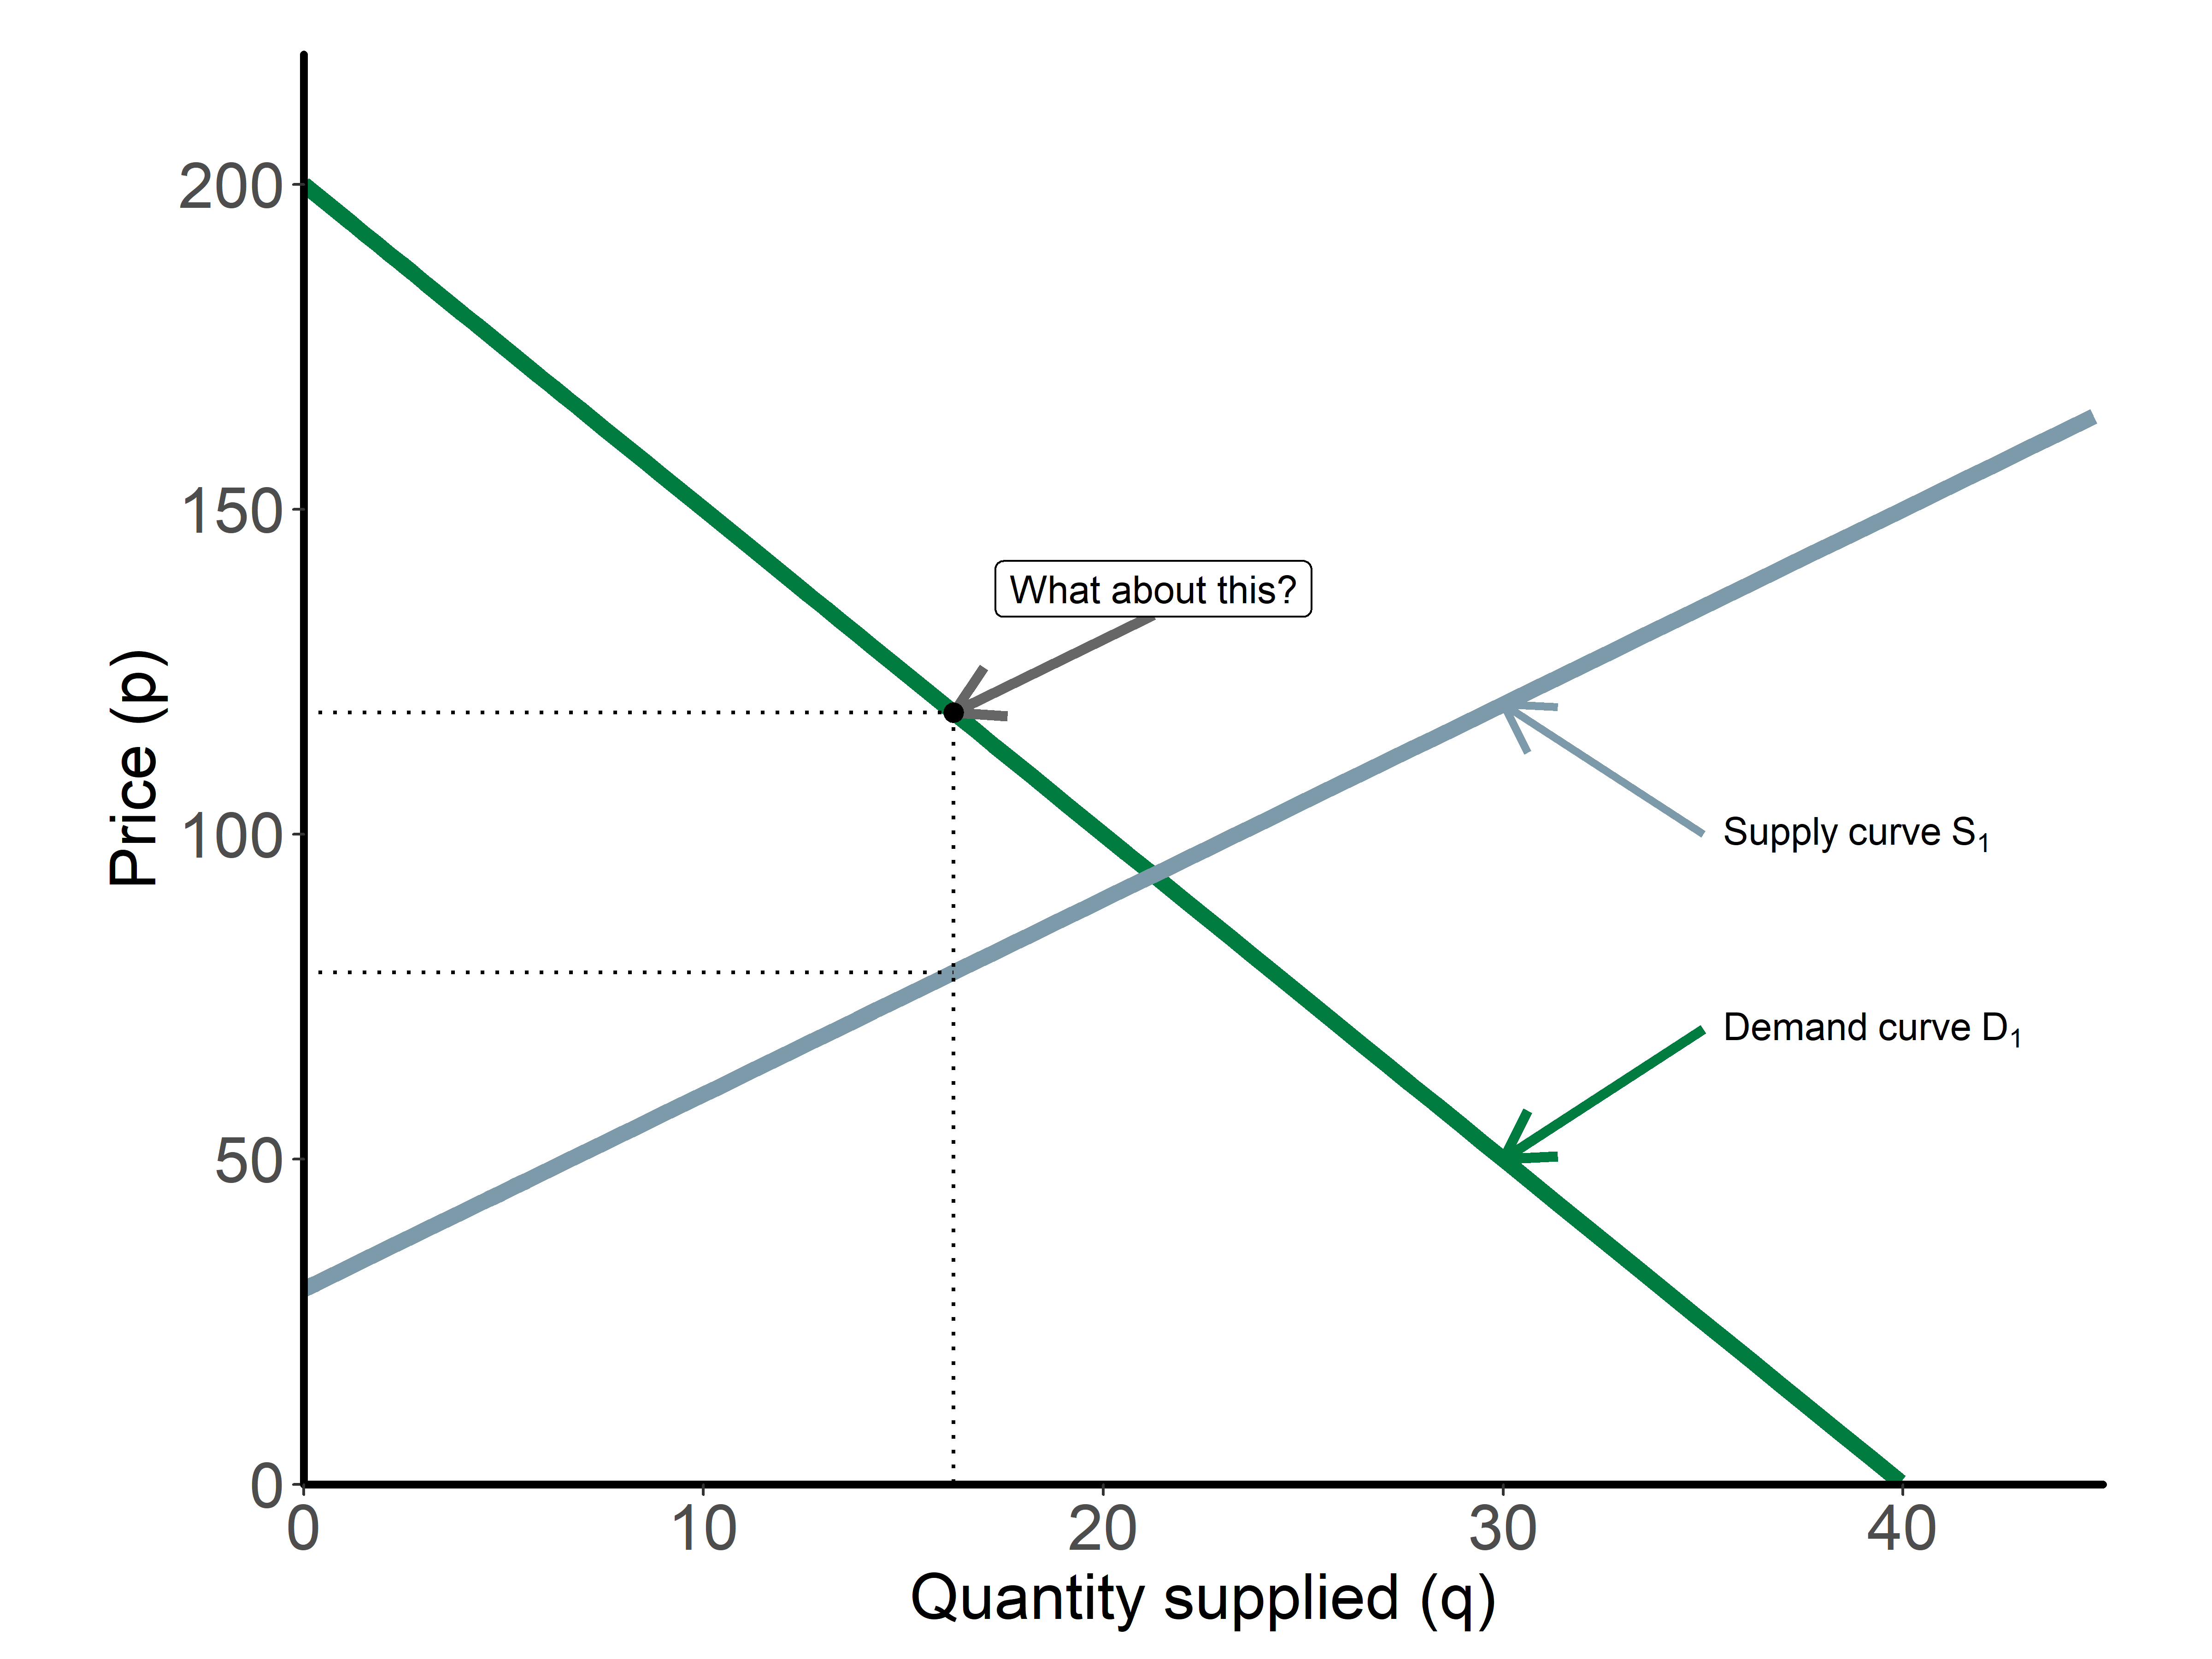
\includegraphics[width=\textwidth]{../images/equil_expl_3.png}
}
\caption{Off-equilibrium points, and the rationale of equilibrium}
\end{figure}
}


\frame{
	\frametitle{Market Equilibrium}
	
		\begin{figure}[t!]
    \center
	\resizebox{!}{.4\linewidth}{
    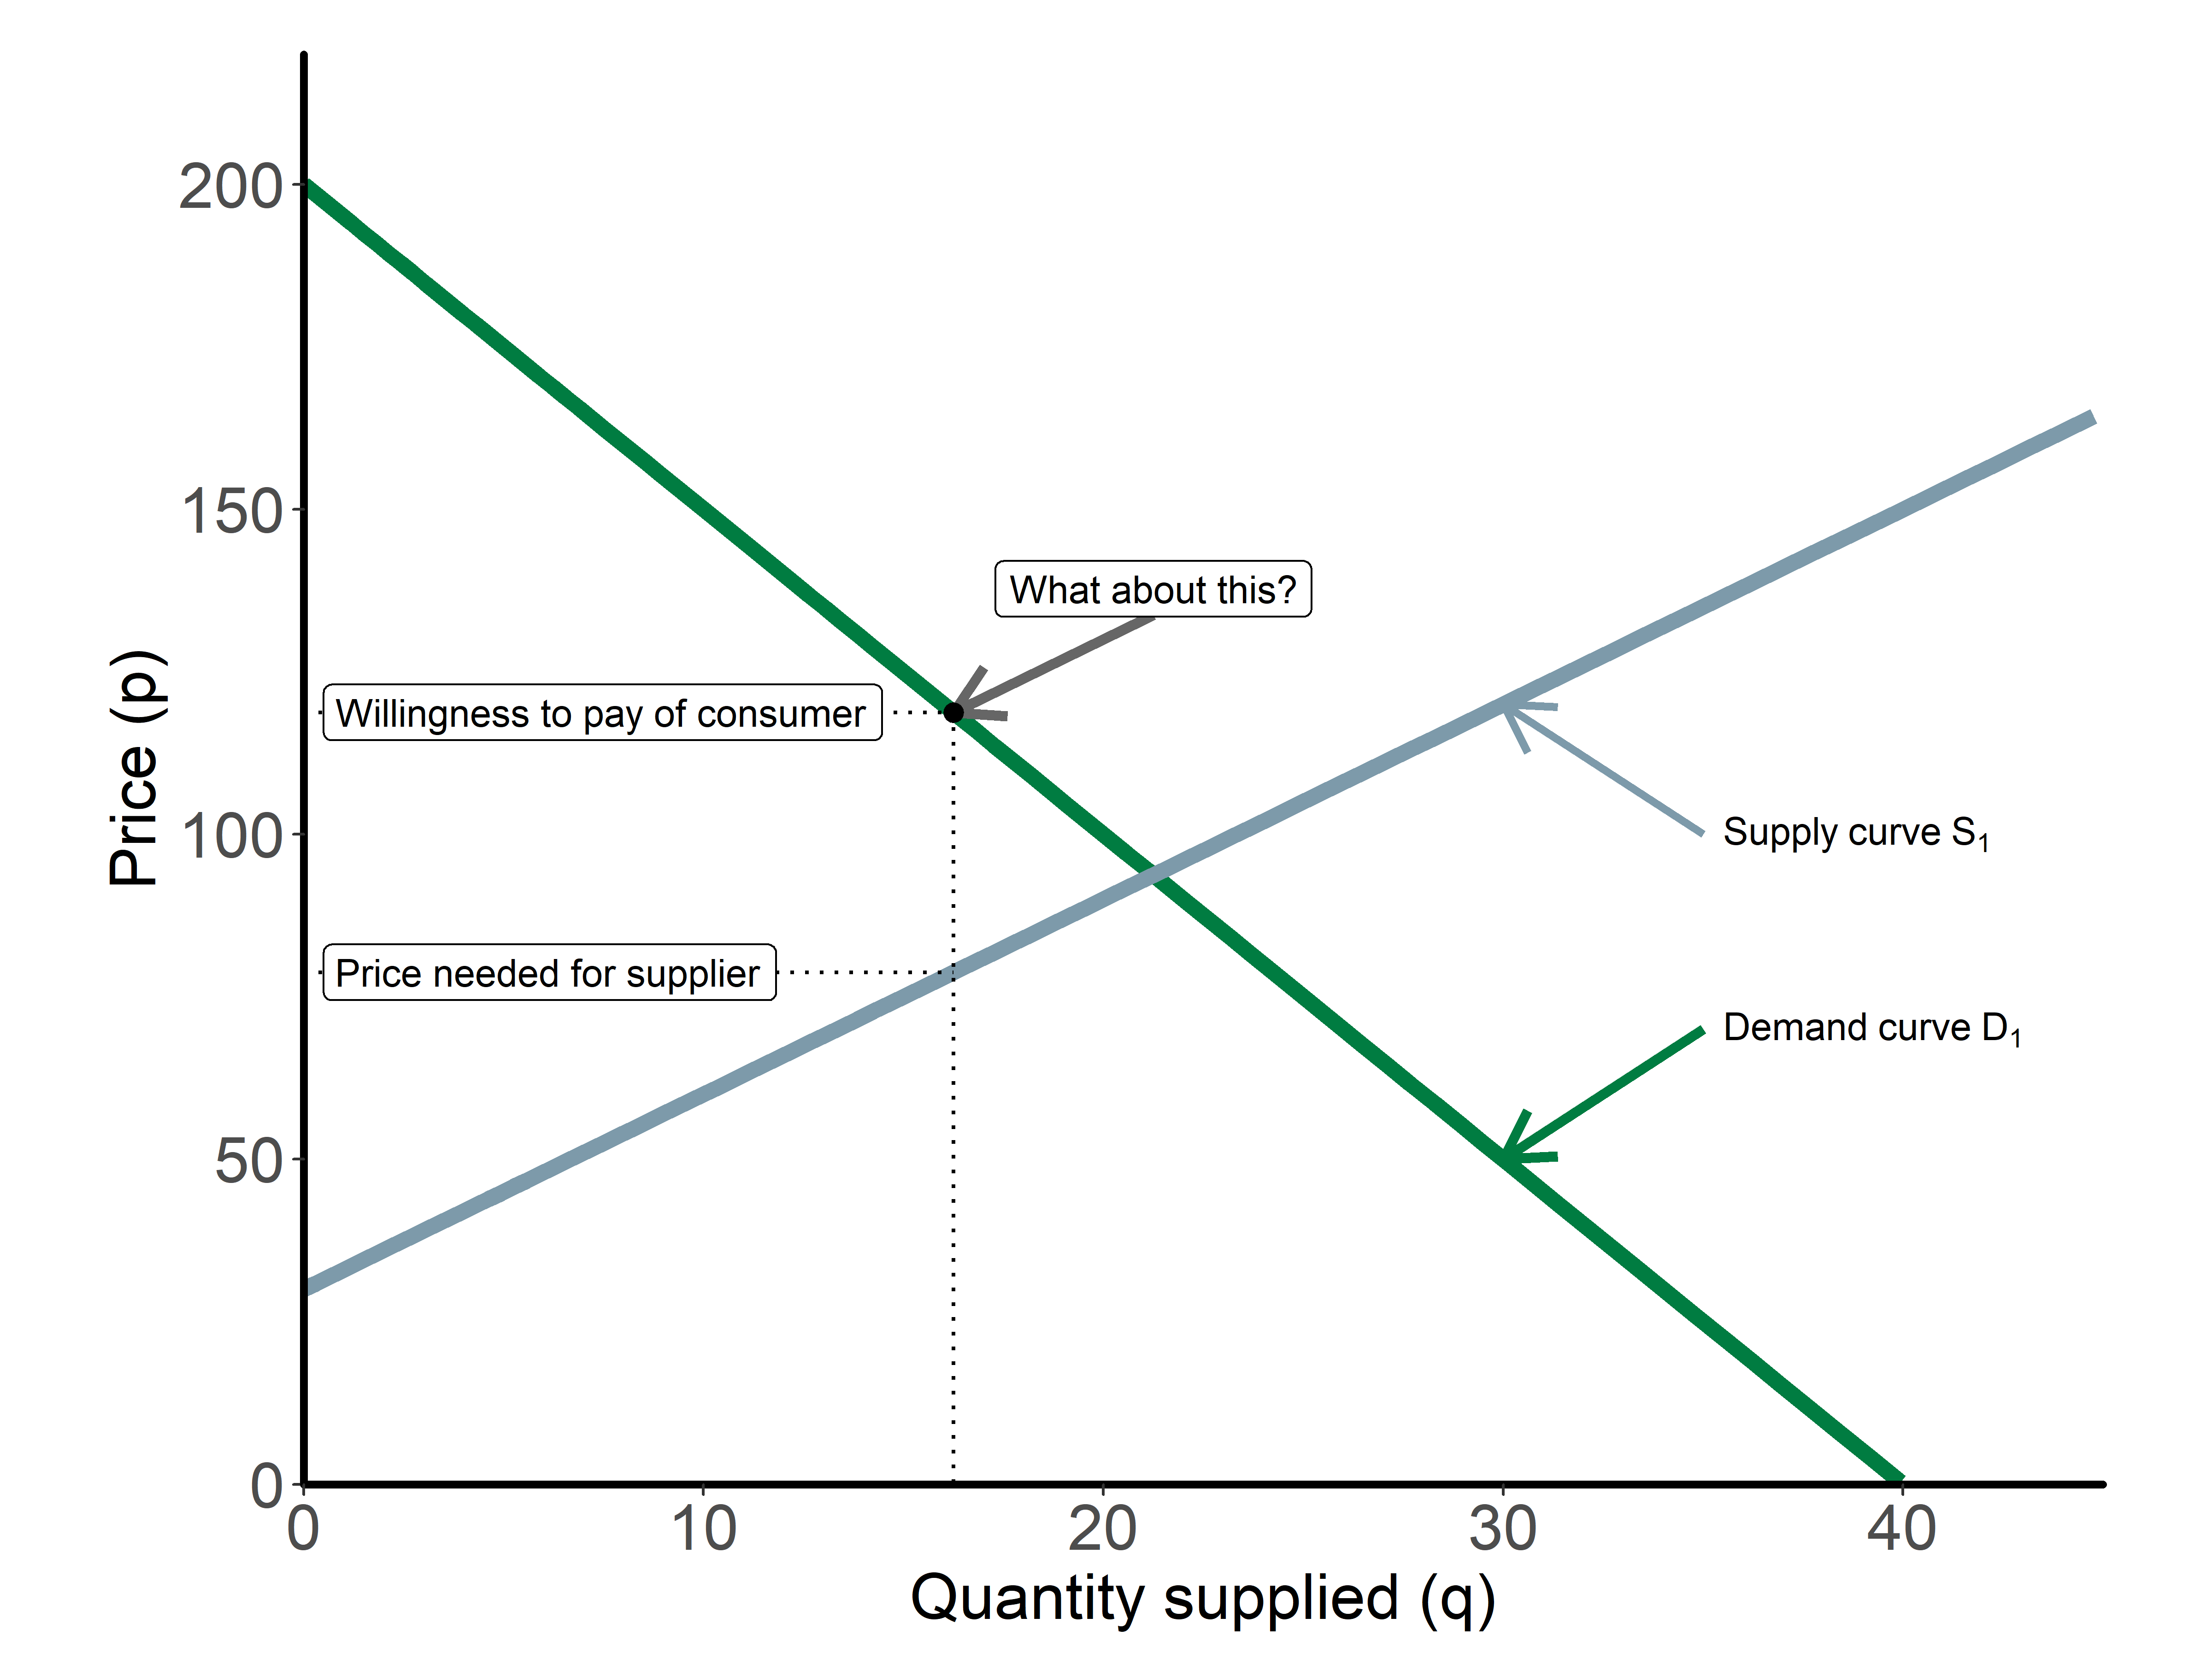
\includegraphics[width=\textwidth]{../images/equil_expl_4.png}
}
\caption{Off-equilibrium points, and the rationale of equilibrium}
\end{figure}
}



\frame{
	\frametitle{Market Equilibrium}
	\begin{itemize}
	\item We can also solve for the market equilibrium analytically using algebra:
		\begin{align*}
		Q_{D} = 40 - \frac{p}{5} \quad \text{and} \quad Q_{S} = \frac{p}{3}-10
		\end{align*}
	\item In equilibrium $Q_{D}=Q_{S}$. Substituting yields:
		\begin{align*}
		40 - \frac{p}{5} &= \frac{p}{3}-10\\
		\frac{8p}{15} &=50 \\
		p &= 93.75
		\end{align*}
	\item Substituting in the equilibrium price into $Q_{D}$ or $Q_{S}$ yields the equilibrium
quantity of 21.25.
	\end{itemize}
}


\frame{
	\frametitle{Market Equilibrium Check}
	\begin{itemize}
	\item We can do the same off-equilibrium checks with algebra too. For example, let's consider whether Q=25 is an equilibrium.
\item Start with the marginal willingness to pay (or demand) at Q=25:
		\begin{align*}
		Q_{D} = 40 - \frac{p}{5} \quad \text{so if} \quad 25 = 40 - \frac{p}{5},\,p\text{ must be }\frac{p}{5}=15,\, p=75
		\end{align*}
	\item But, at p=75, how much are firms willing to supply?
		\begin{align*}
		Q_{S} = \frac{75}{3}-10,\,\text{so }Q_{S} &= 15
		\end{align*}
	\item So, at a quantity of Q=25, the marginal consumer who sets the price is willing to pay p=75, but at a price of p=75, there's only going to be a supply of Q=15. This cannot be an equilibrium.
	\end{itemize}

}

\frame{
	\frametitle{Market Equilibrium}
	Remember this graph? Same thing as the algebra in the previous slide
		\begin{figure}[t!]
    \center
	\resizebox{!}{.4\linewidth}{
    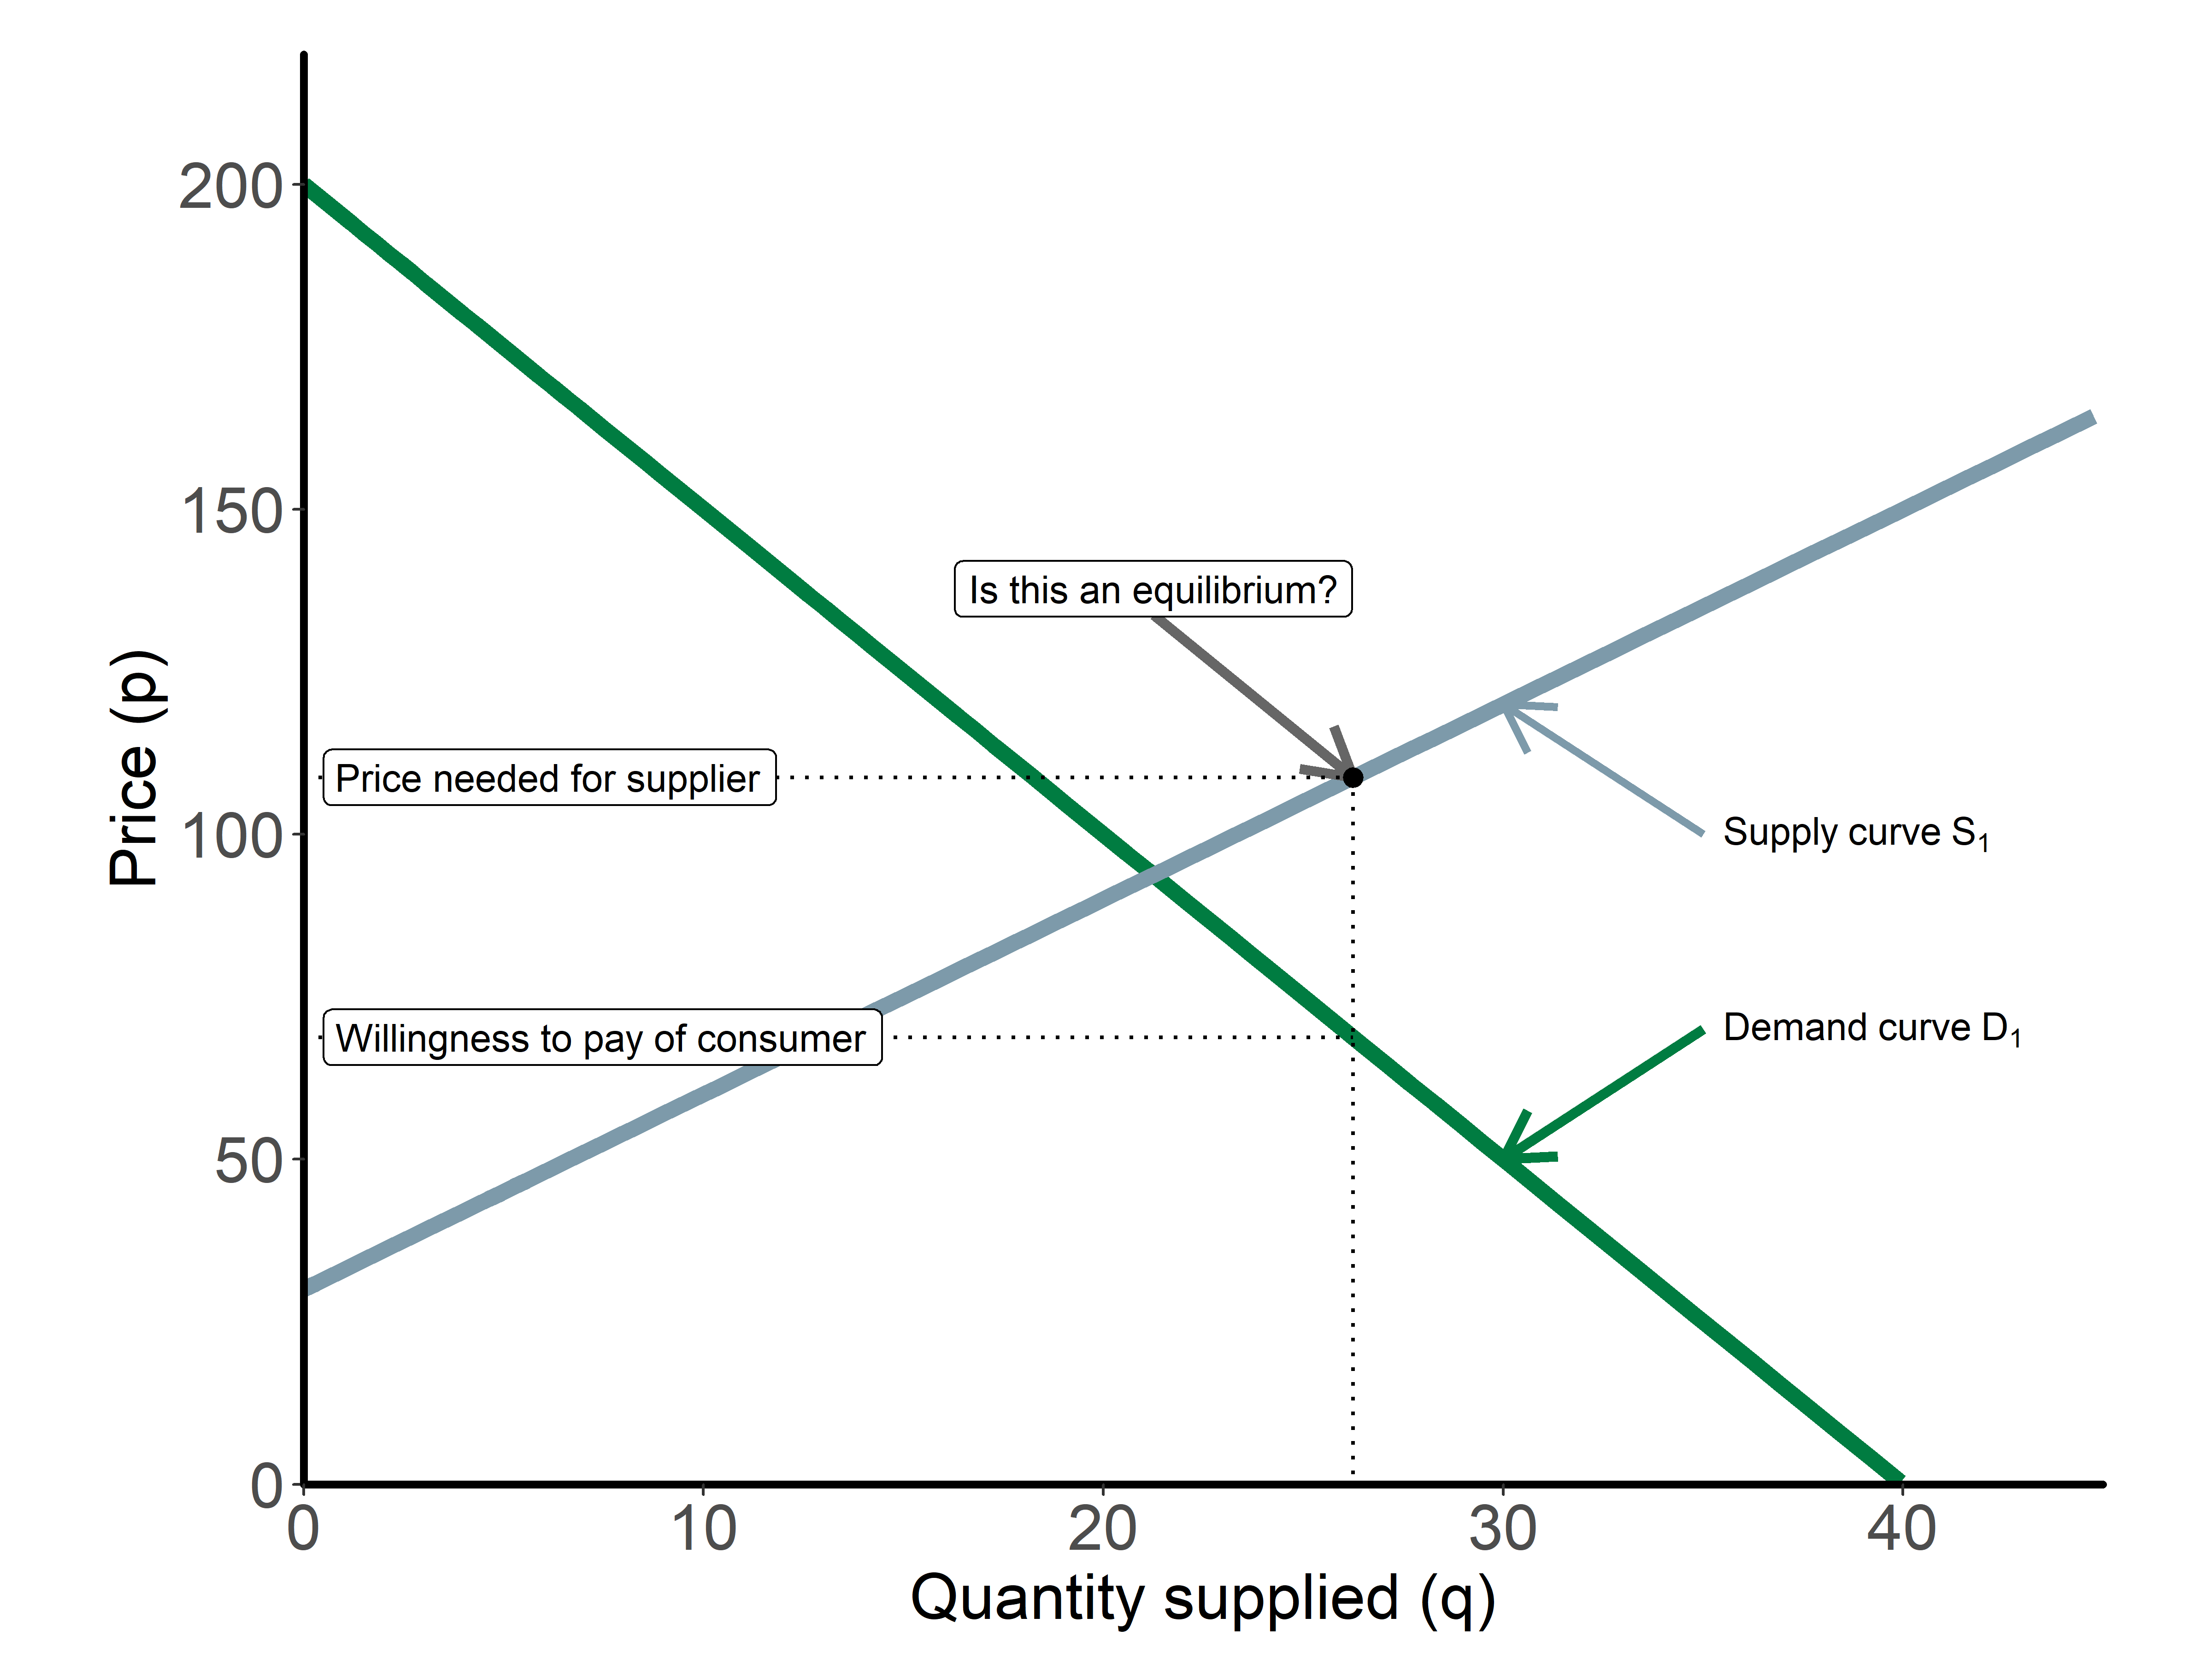
\includegraphics[width=\textwidth]{../images/equil_expl_2.png}
}
\caption{Off-equilibrium points, and the rationale of equilibrium}
\end{figure}
}



\section{Deriving Predictions from the Model}

\frame{
	\frametitle{Shifts in Equilibrium}
	\begin{itemize}
	\item The supply-and-demand model tells us the price and quantity that will \textit{clear the
market} holding all other factors fixed.
	\item Changes in these other factors will change the market equilibrium by shifting the supply
and demand curves (or both!).
	\item We can use the model to precisely predict how changes in these other factors will alter the
market equilibrium.
	\item We will consider two sets of factors:
		\begin{enumerate}
		\item \textit{Market fundamentals}, e.g. inputs, preferences, technology, etc.
		\item Government intervention.
		\end{enumerate}
	\end{itemize}
}

\frame{
	\frametitle{Using the Model: Shifts in Demand}
	\begin{itemize}
	\item We will start by considering the effects of an increase in annual household income.
	\item Specifically, suppose that household income increases from \$100,000 to \$120,000.
	\item How does this affect equilibrium price and quantity?
    \item Recall that our demand function was:
		\begin{align*}
		Q = 30 - \frac{p}{5} + 0.1 Y
		\end{align*}
where Y is income in thousands of dollars
	\end{itemize}
}

\frame{
	\frametitle{Using the Model: Shifts in Demand}
	\begin{itemize}
	\item In the previous examples, we didn't invert demand with income left as a variable, but we can do so:
		\begin{align*}
		Q &= 30 - \frac{p}{5} + 0.1 Y\\
        5Q &= 150 - p + 0.5 Y\\
        p&=150+0.5Y-5Q
		\end{align*}
\item In the previous examples, we generally used $Y=100$, at which the inverse demand reduces to our familiar $p=200-5Q$. At income of $Y=120$, $p=210-5Q$
	\end{itemize}
}



\frame{
	\frametitle{Shifts in Equilibrium: Shifting Demand}
	%	The demand for gasoline:
	
	\begin{figure}[t!]
    \center
	\resizebox{!}{.4\linewidth}{
    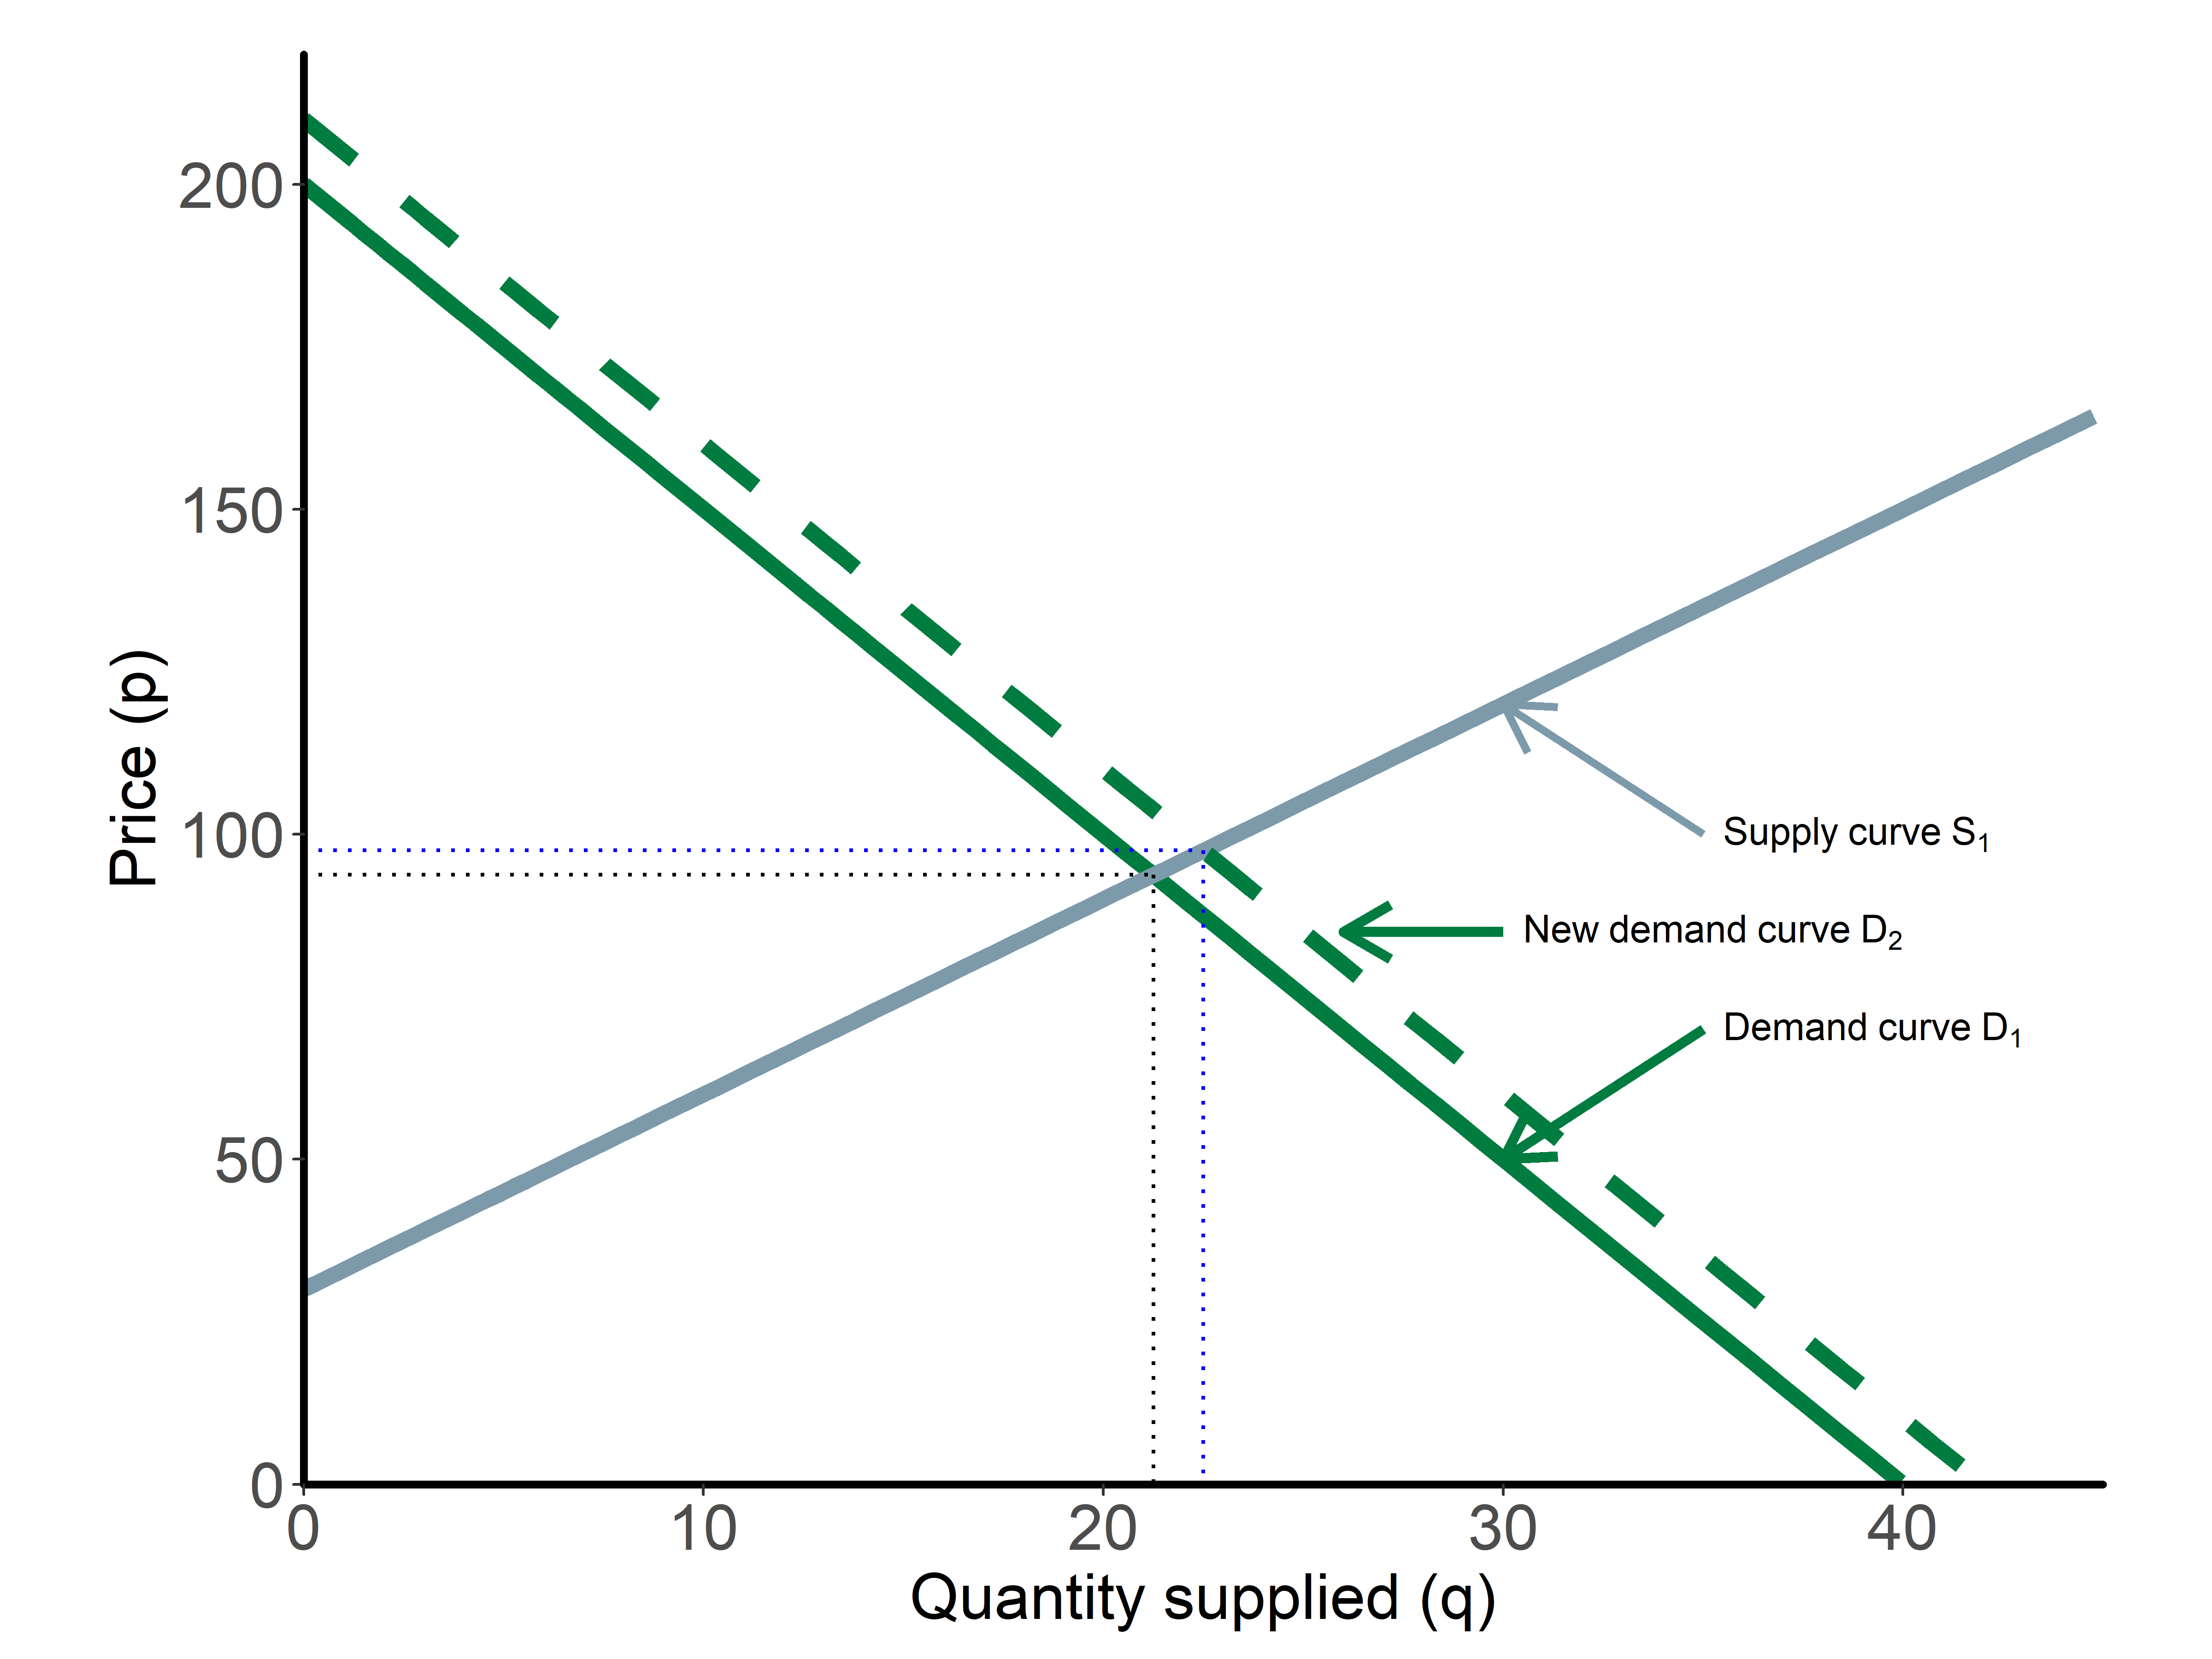
\includegraphics[width=\textwidth]{../images/equil_shift_income.png}
}
\caption{The effects of an increase in income}
\end{figure}
}

\frame{
	\frametitle{Shifts in Equilibrium: Shifting Demand}
	\begin{itemize}
	\item The increase in income shifts the demand curve to the right (from $D_{1}$ to $D_{2}$).
	\item[]
	\item This results in a \textit{movement along the supply curve}.
	\item[]
	\item Why?
	\end{itemize}
}

\frame{
	\frametitle{Shifts in Equilibrium: Shifting Demand}
	%	The demand for gasoline:
	
	\begin{figure}[t!]
    \center
	\resizebox{!}{.4\linewidth}{
    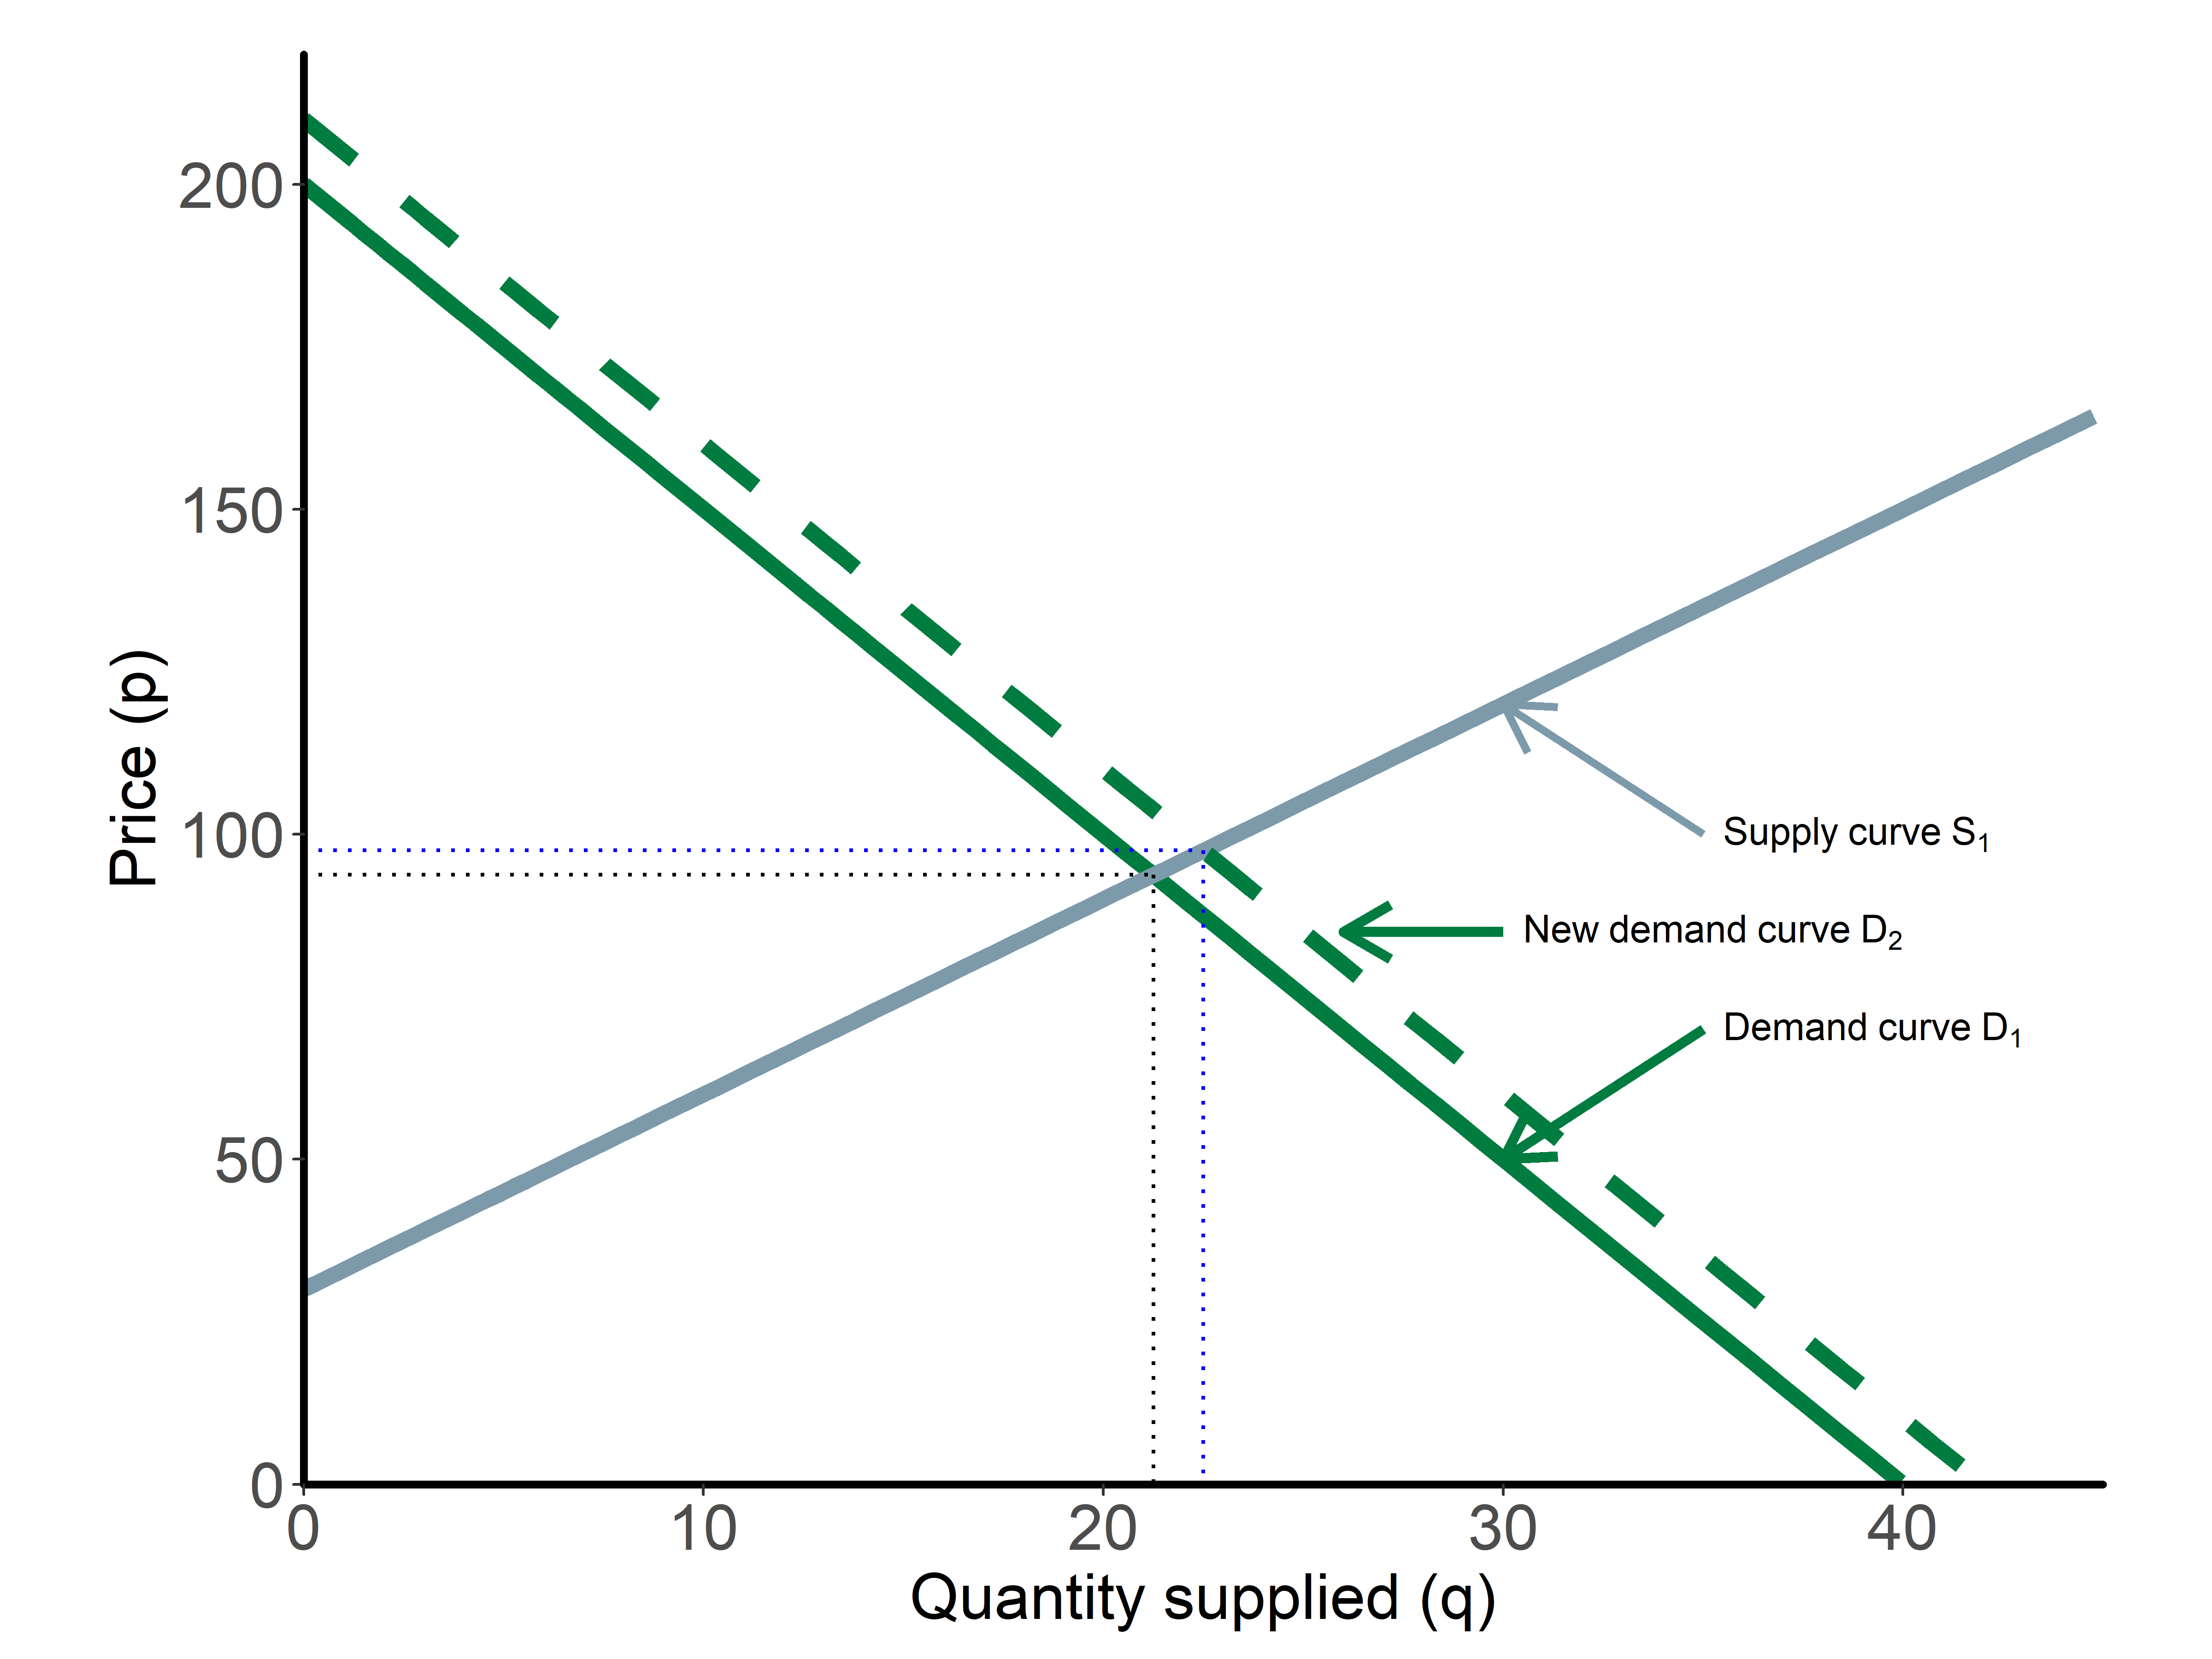
\includegraphics[width=\textwidth]{../images/equil_shift_income.png}
}
\caption{The effects of an increase in income}
\end{figure}
}

\frame{
	\frametitle{Shifts in Equilibrium: Shifting Demand}
	%	The demand for gasoline:
	
	\begin{figure}[t!]
    \center
	\resizebox{!}{.4\linewidth}{
    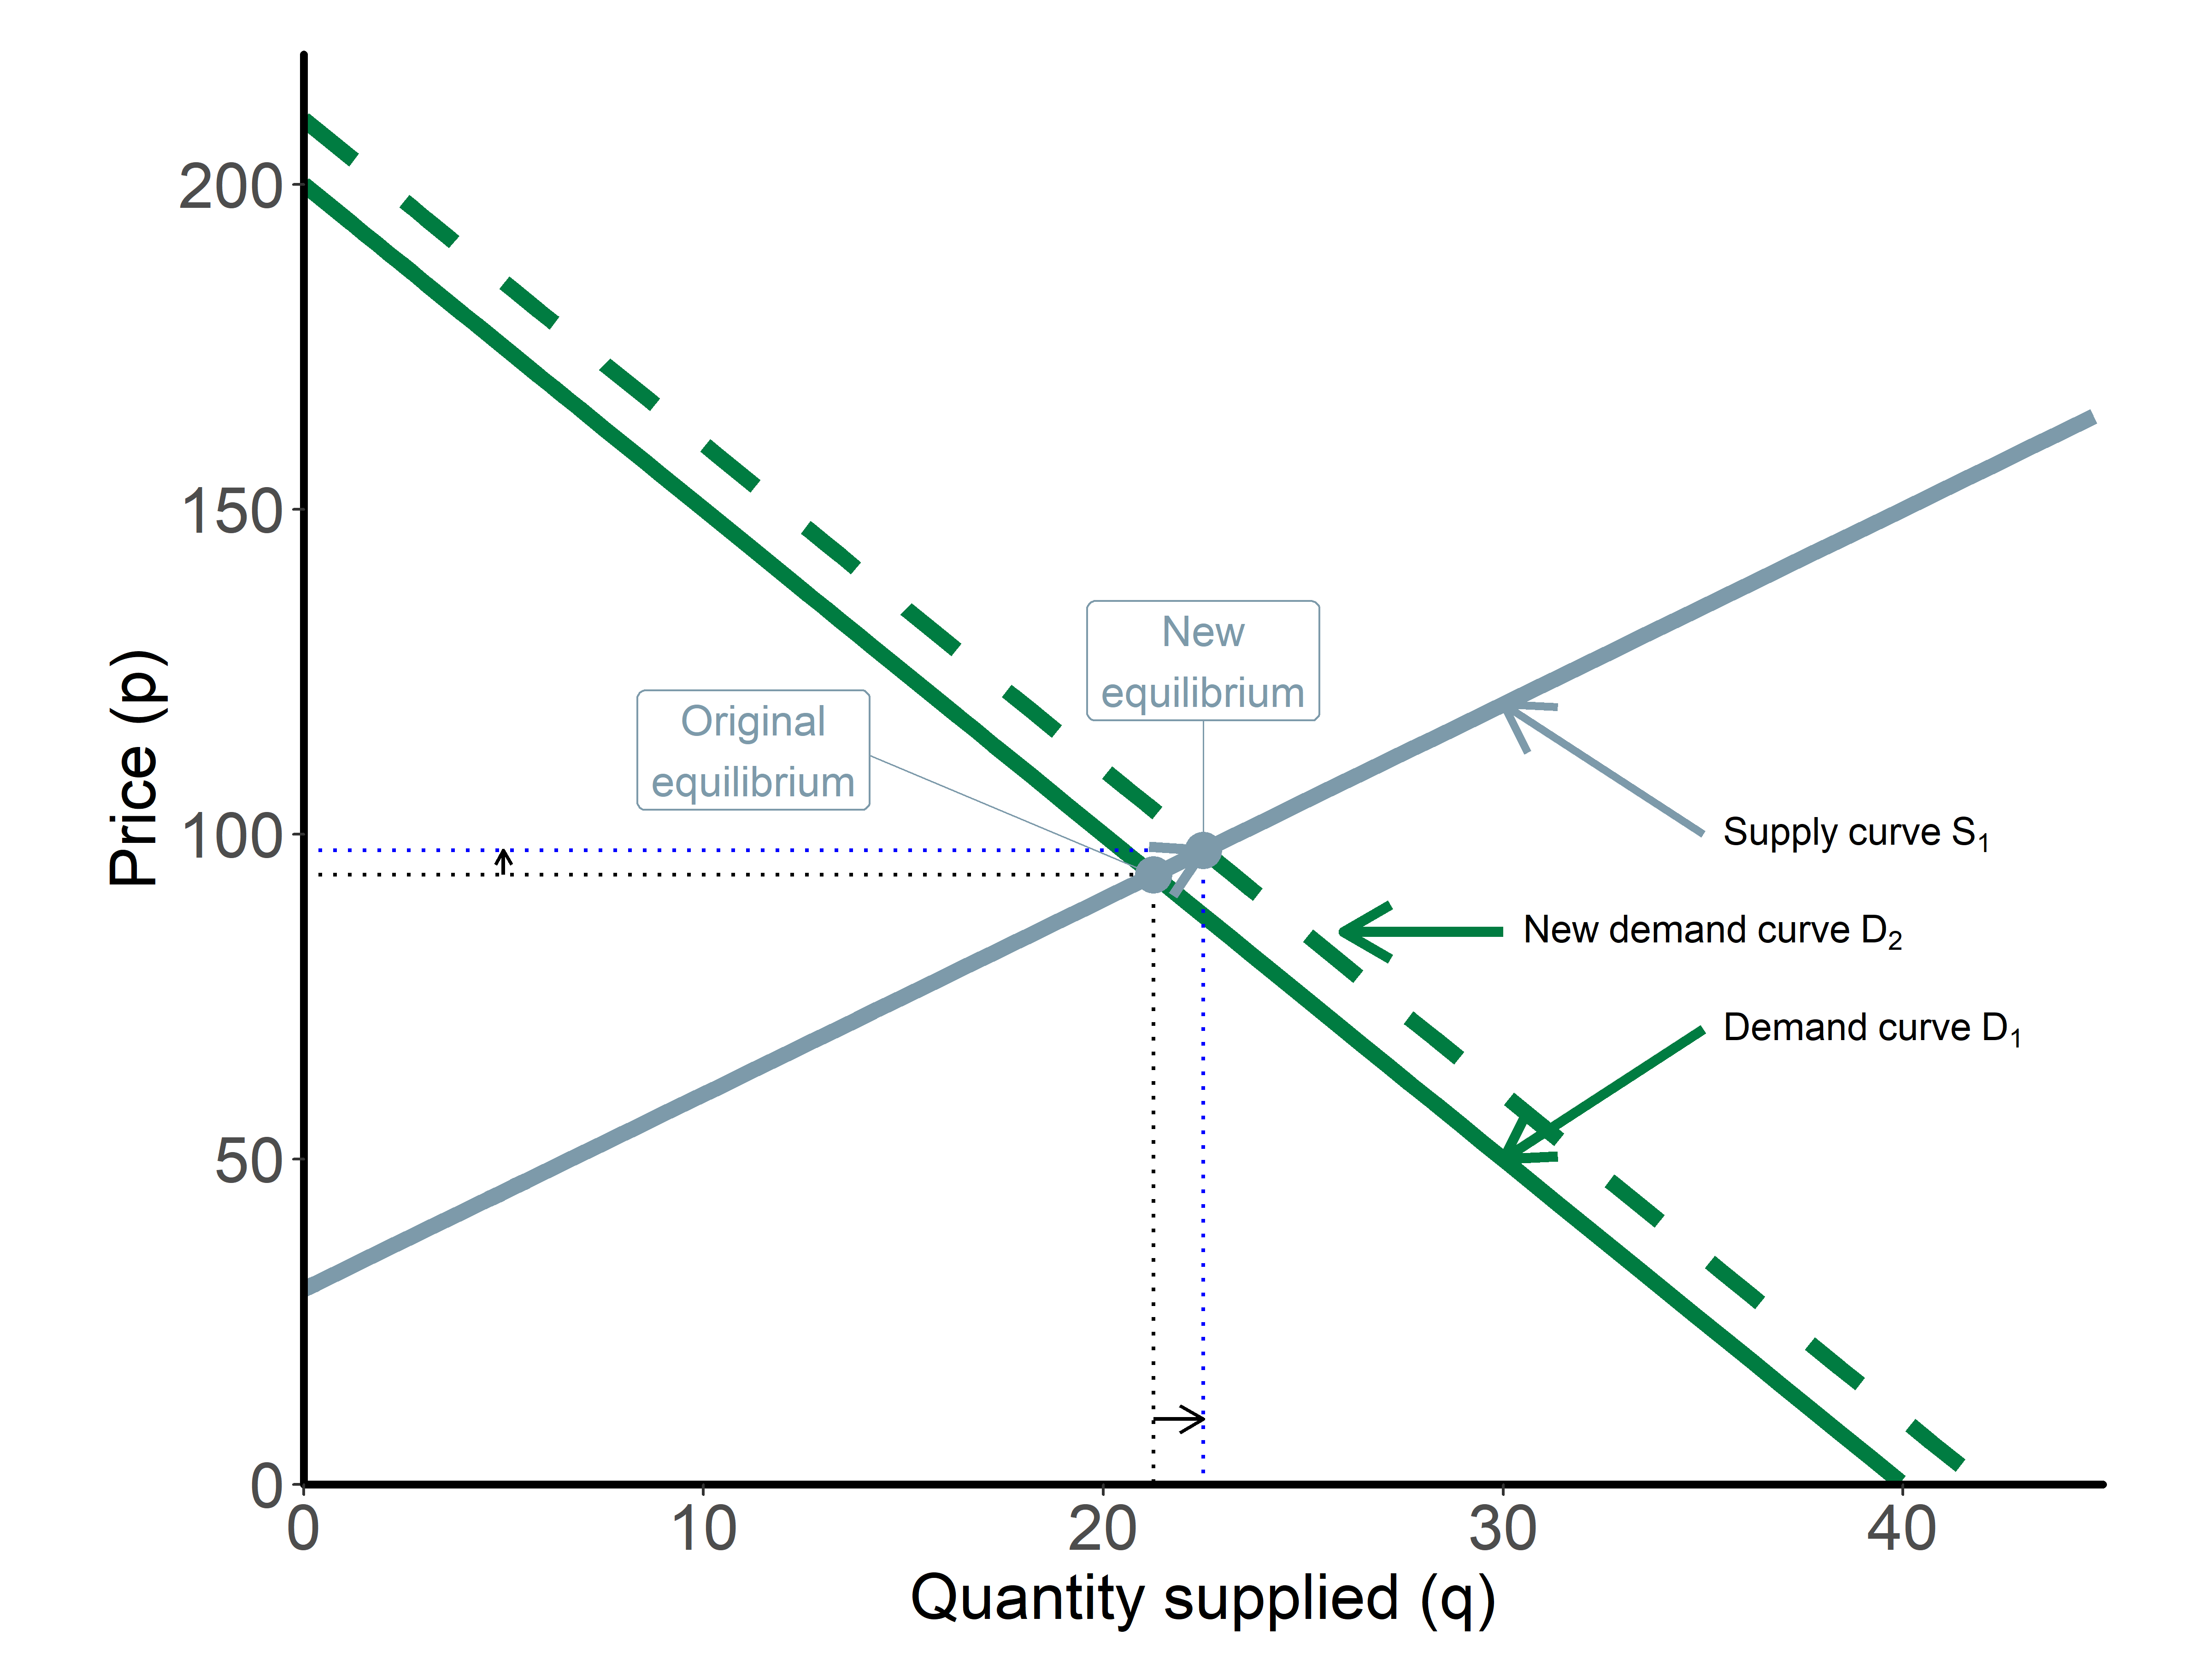
\includegraphics[width=\textwidth]{../images/equil_shift_mvmt1.png}
}
\caption{The effects of an increase in income}
\end{figure}
}



\frame{
	\frametitle{Shifts in Equilibrium: Shifting Demand}
	\begin{itemize}
	\item We can also solve for the change in market equilibrium prices and quantities analytically using algebra. Recall our initial calculations:
		\begin{align*}
		Q_{D} = 40 - \frac{p}{5} \quad \text{and} \quad Q_{S} = \frac{p}{3}-10
		\end{align*}
	\item In equilibrium $Q_{D}=Q_{S}$. Substituting yields:
		\begin{align*}
		40 - \frac{p}{5} &= \frac{p}{3}-10\\
		\frac{8p}{15} &=50 \, \rightarrow	p &= 93.75
		\end{align*}
	\item Substituting $p=93.75$ into $Q_{D}$ or $Q_{S}$ yields $Q=21.25$.
	\end{itemize}
}


\frame{
	\frametitle{Shifts in Equilibrium: Shifting Demand}
	\begin{itemize}
	\item Recall that the underlying demand function was $Q = 30 - \frac{p}{5} + 0.1 Y$, so with income of \$120,000, or $Y=120$:
		\begin{align*}
		Q_{D} = 30 - \frac{p}{5} +.1(120) \quad \text{and} \quad Q_{S} = \frac{p}{3}-10
		\end{align*}
	\item In equilibrium $Q_{D}=Q_{S}$. Substituting yields:
		\begin{align*}
		42 - \frac{p}{5} &= \frac{p}{3}-10\\
		\frac{8p}{15} &=52 \, \rightarrow  p = 97.5\\
		\end{align*}
	\item Substituting $p = 97.5$ into $Q_{D}$ or $Q_{S}$ yields $Q=22.5$.
	\end{itemize}
}






\frame{
	\frametitle{Shifts in Equilibrium: Shifting Demand}
	\begin{itemize}
	\item And now we can compare the impacts of a shift in demand caused by a change in income. In the initial equilibrium:
		\begin{align*}
		Q_{1}^* & = 21.25\\
		p_{1}^* & = 93.75
		\end{align*}
	\item In the \underline{new} equilibrium after the shift in income.
		\begin{align*}
		Q_{2}^* & = 22.5\\
		p_{2}^* & = 97.50
		\end{align*}
	\item The \underline{change} in income leads to a \underline{shift in demand}, and a \underline{movement along the supply curve} such that:
		\begin{align*}
		\Delta_p&=3.75\\
        \Delta_Q&=1.25
		\end{align*}
	\end{itemize}
}

\frame{
	\frametitle{Shifts in Equilibrium: Shifting Demand}
	%	The demand for gasoline:
	
	\begin{figure}[t!]
    \center
	\resizebox{!}{.4\linewidth}{
    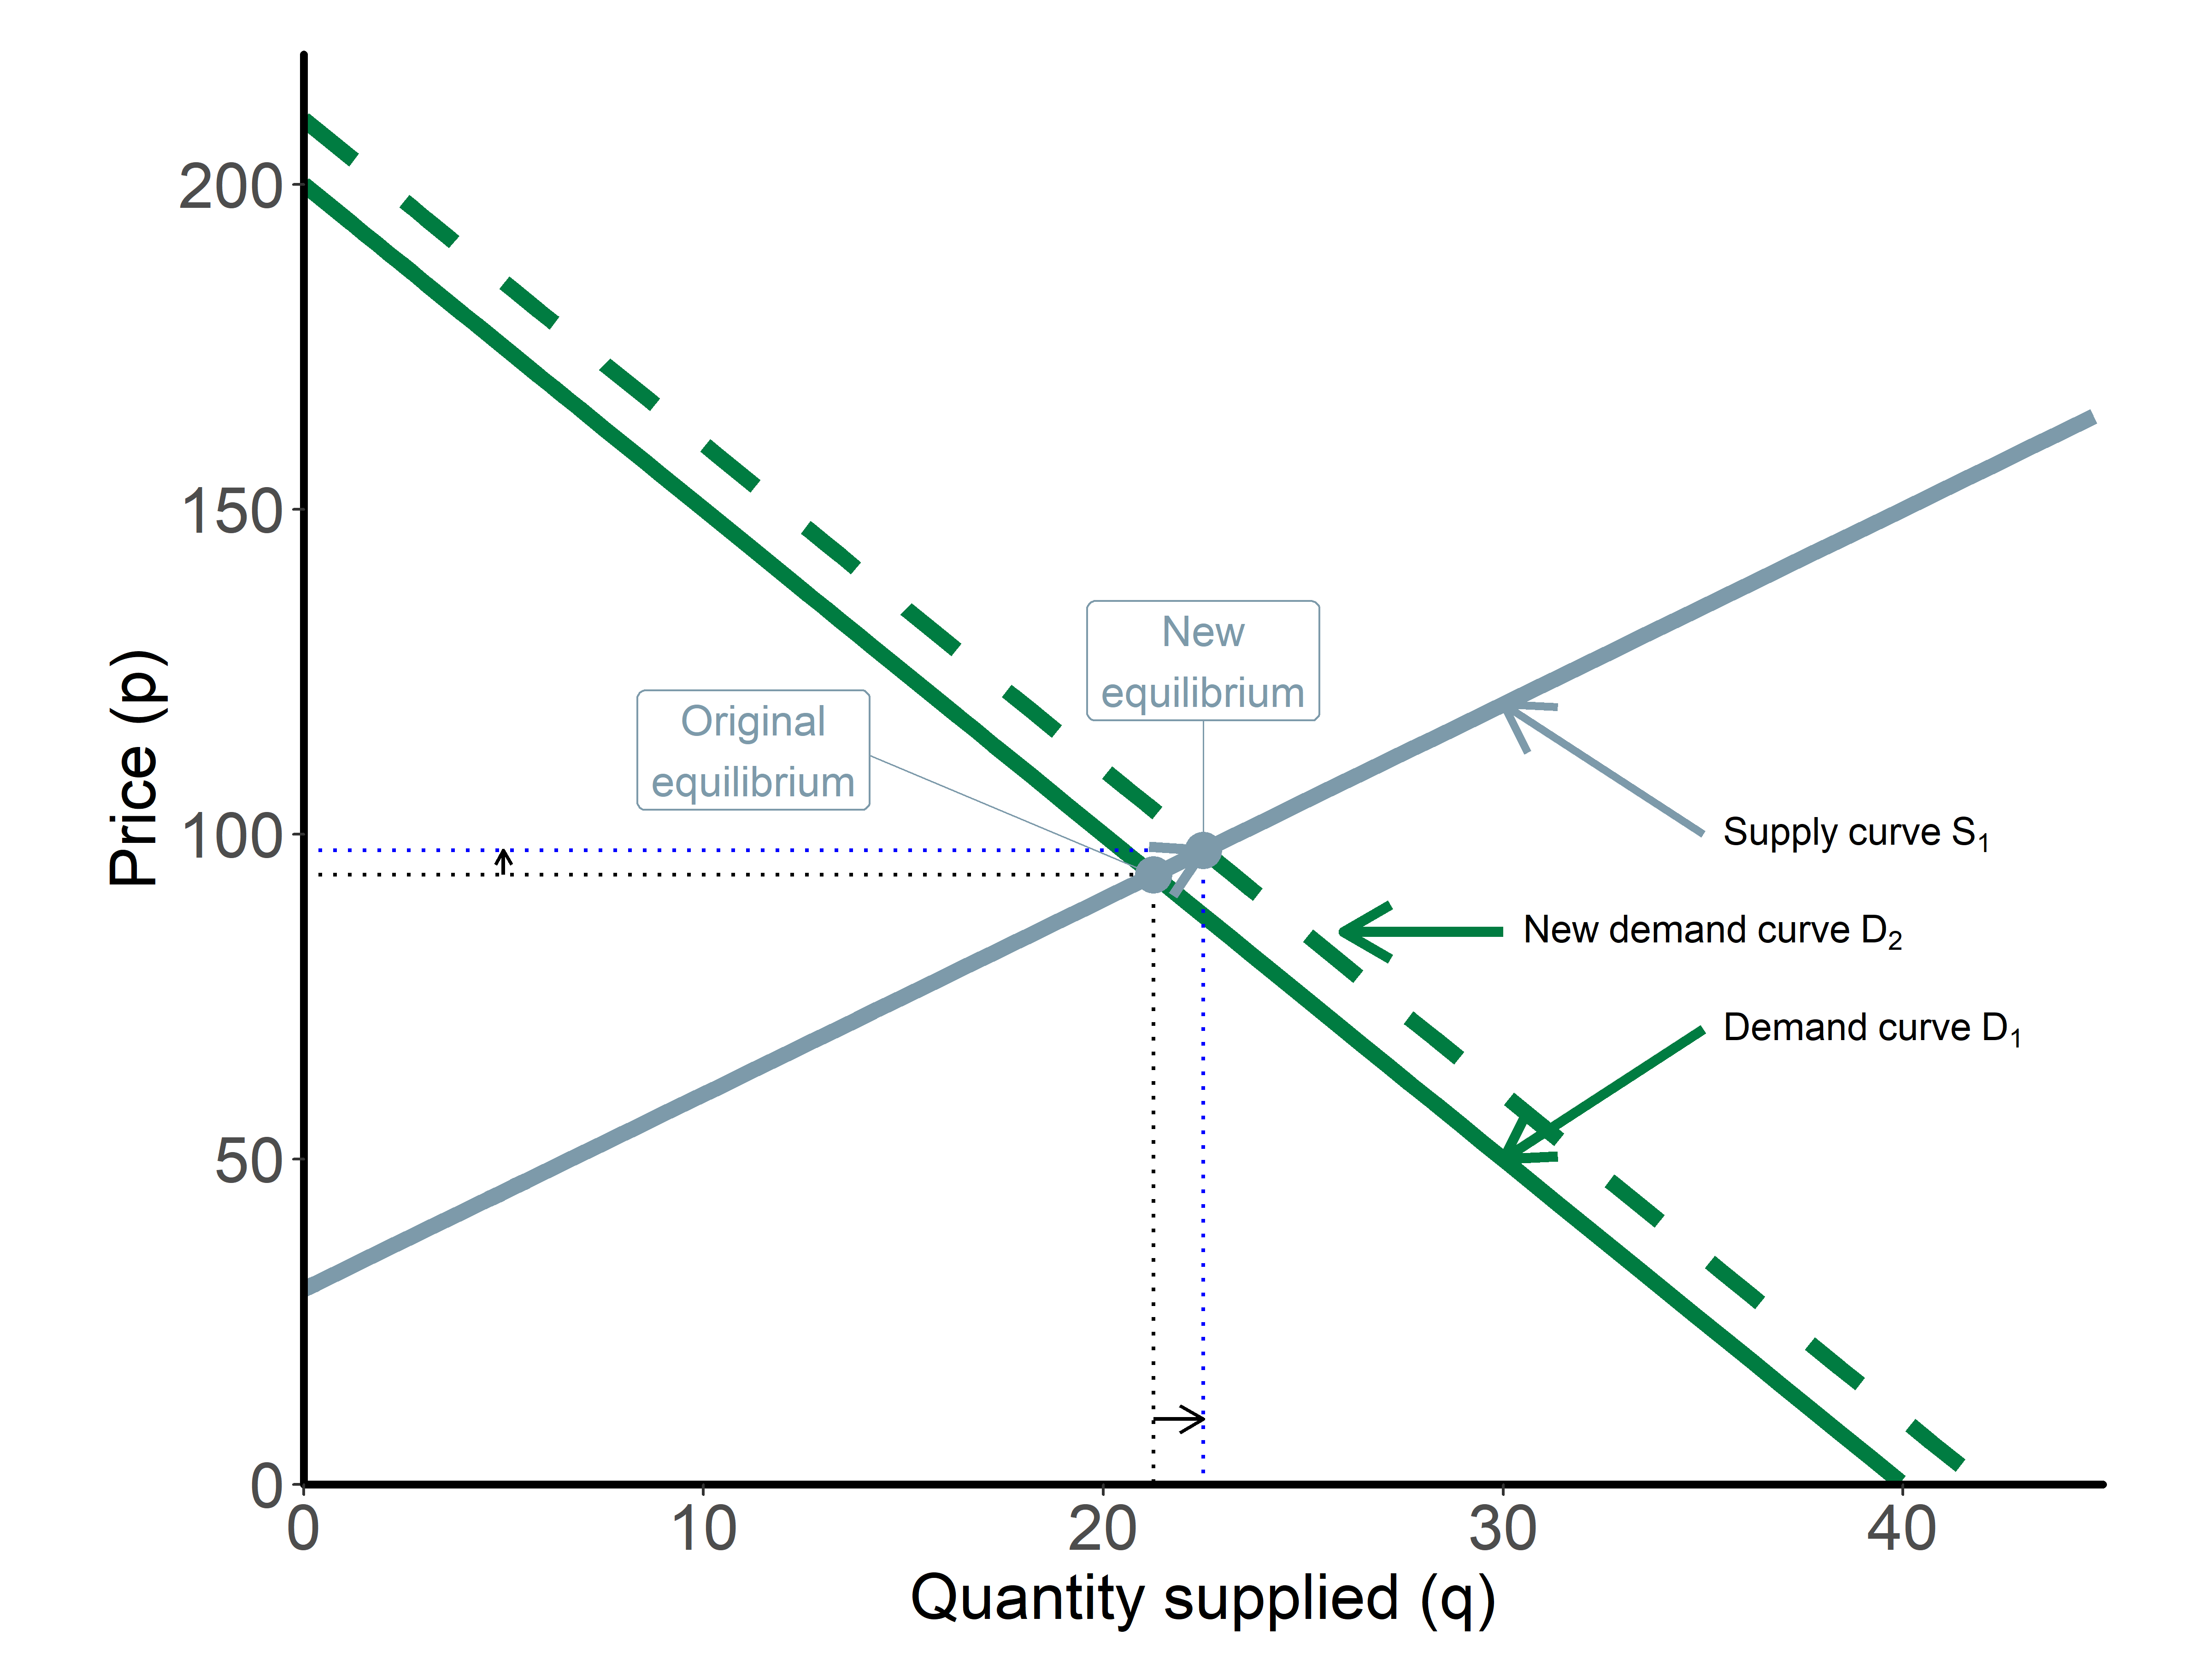
\includegraphics[width=\textwidth]{../images/equil_shift_mvmt1.png}
}
\caption{The effects of an increase in income}
\end{figure}
}



\frame{
	\frametitle{Shifts in Equilibrium: Shifting Supply}
	\begin{itemize}
	\item Suppose instead that the price of crude oil increases from \$40 to \$60 per barrel.
	\item[]
	\item How does this affect equilibrium price and quantity?
	\end{itemize}
}

\frame{
	\frametitle{Shifts in Equilibrium: Shifting Supply}
	%	The demand for gasoline:
	\begin{figure}[t!]
    \center
	\resizebox{!}{.4\linewidth}{
    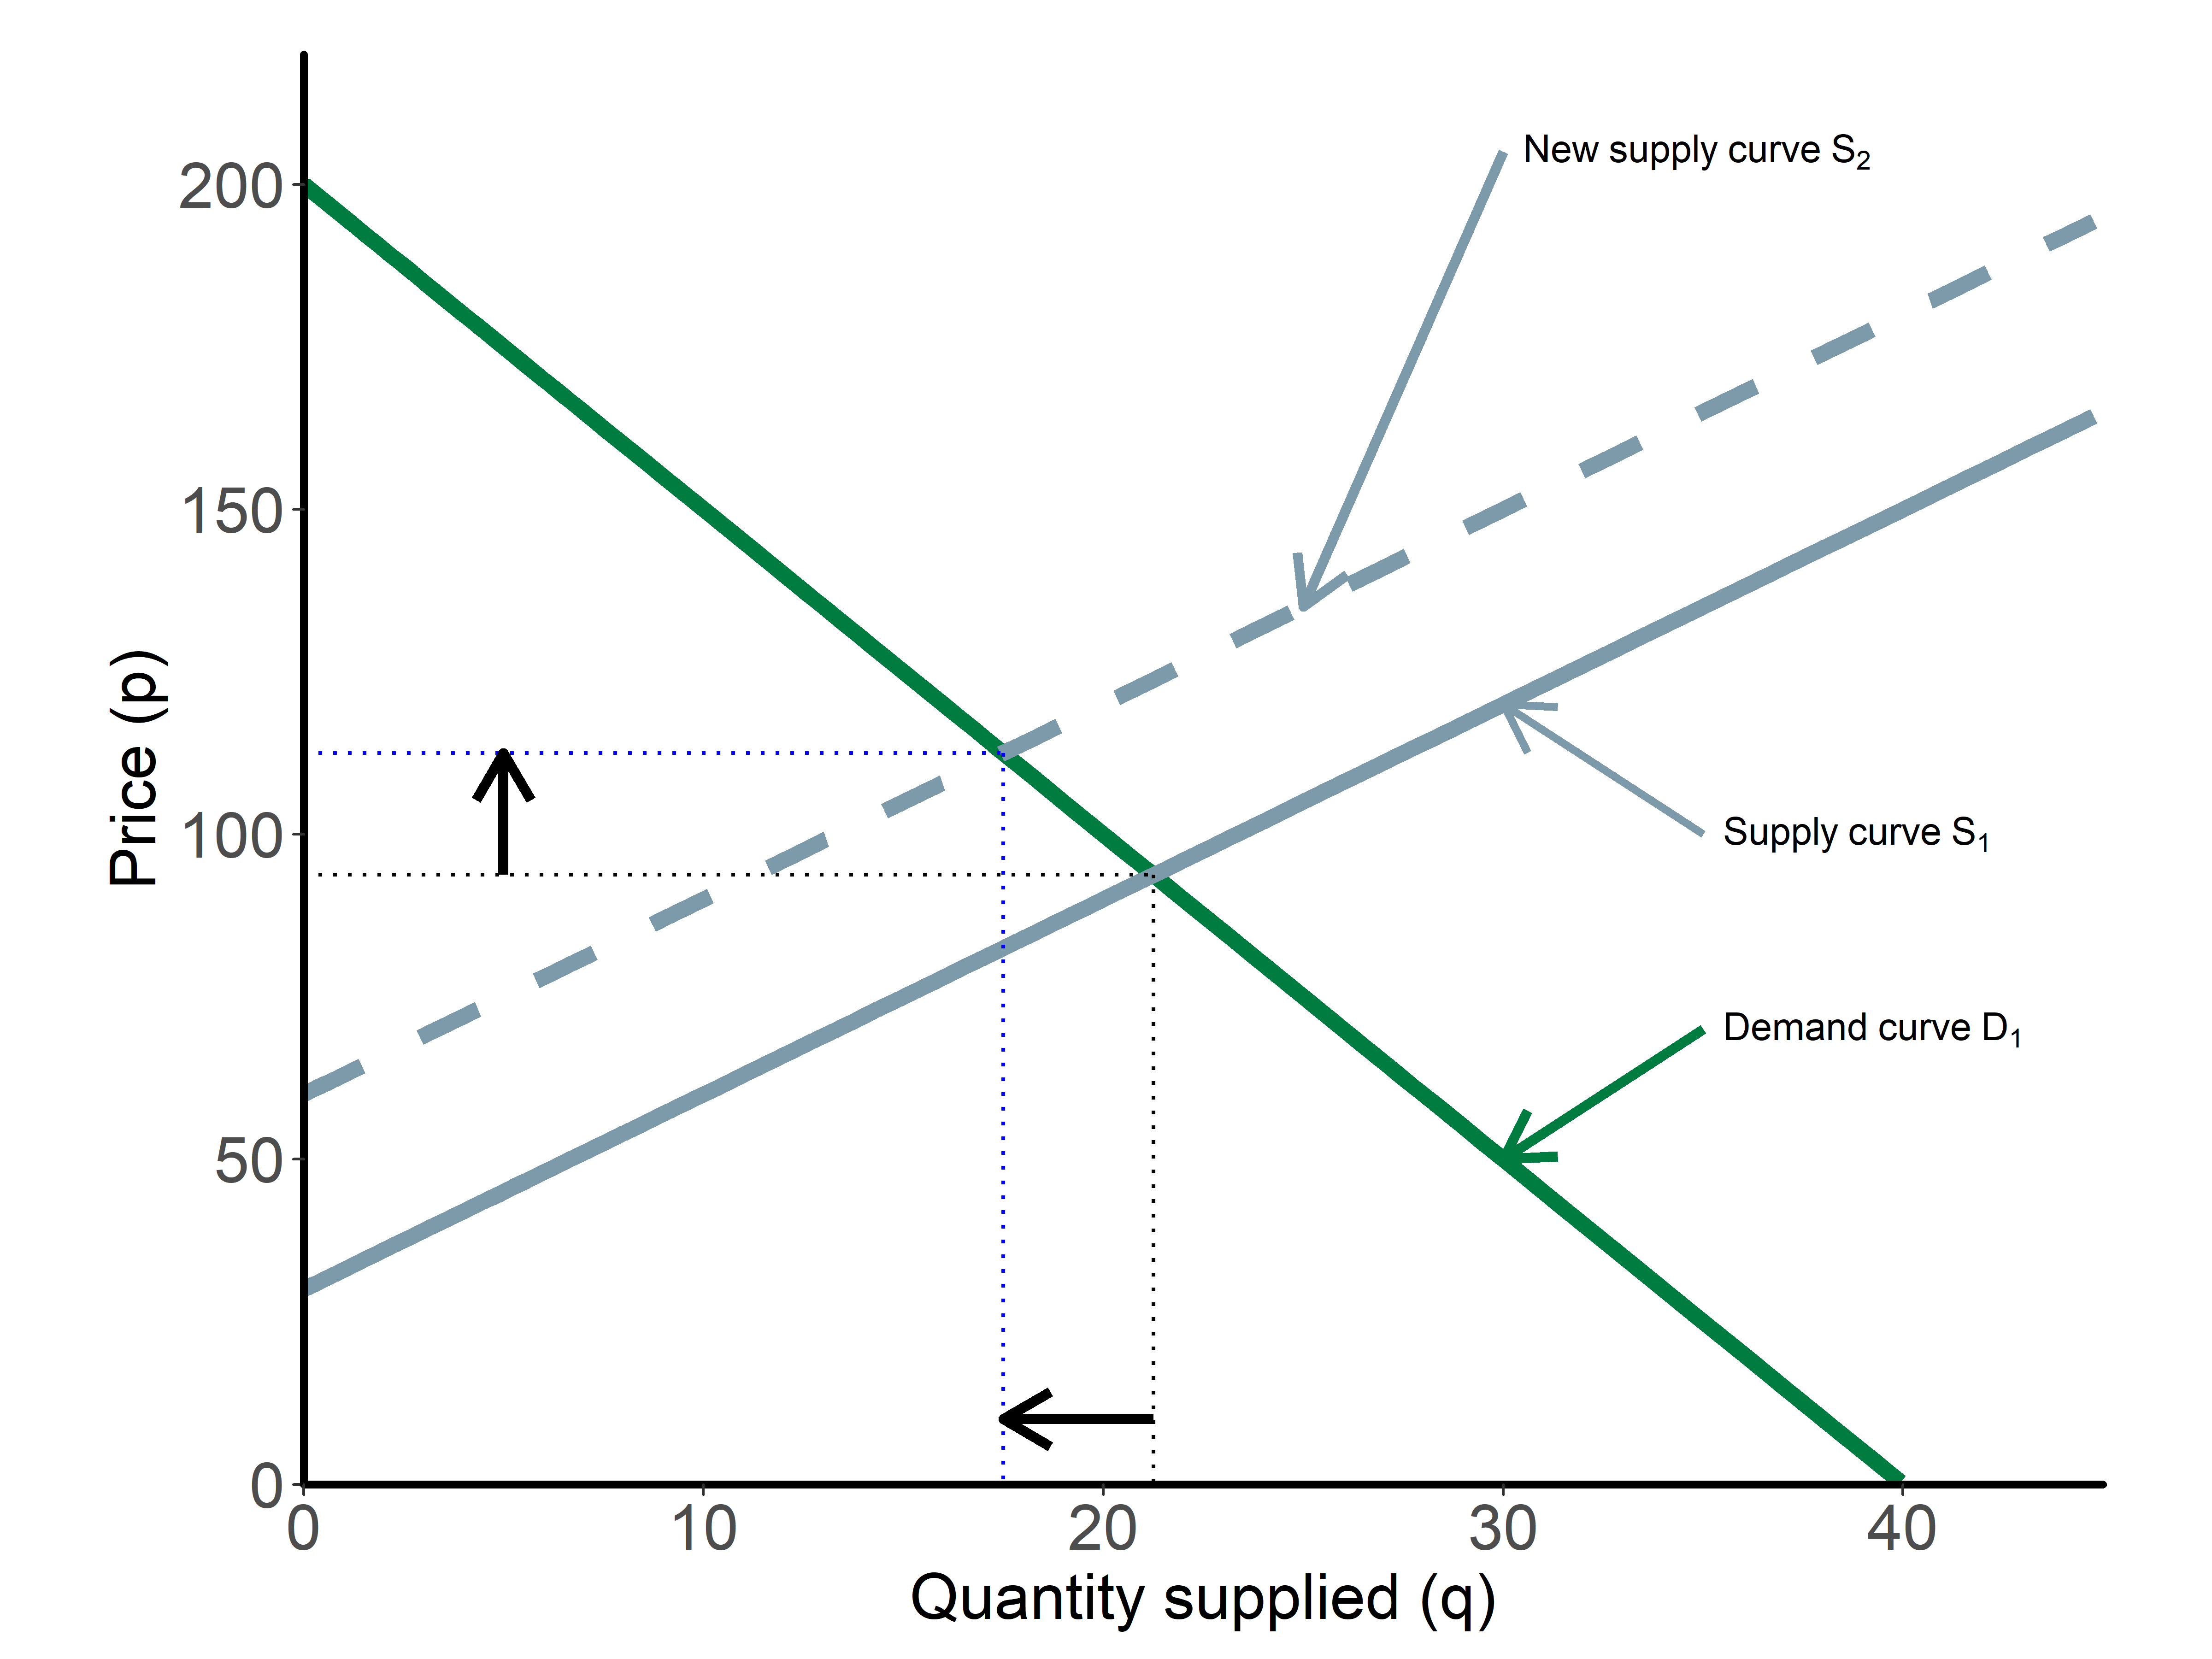
\includegraphics[width=\textwidth]{../images/equil_shift_crude.png}
}

	
\caption{The effects of an increase in the price of crude on gasoline market equilibrium}
\end{figure}
}

\frame{
	\frametitle{Shifts in Equilibrium: Shifting Supply}
	\begin{itemize}
	\item The increase in the price of crude oil (the key input to gasoline production) shifts the supply crude to the left (from $S_{1}$ to
$S_{2}$).
	\item[]
	\item This results in a \textit{movement along the demand curve}.
	\item[]
	\item Why?
	\end{itemize}
}

\frame{
	\frametitle{Shifts in Equilibrium: Shifting Supply}
	%	The demand for gasoline:
	
	\begin{figure}[t!]
    \center
	\resizebox{!}{.4\linewidth}{
    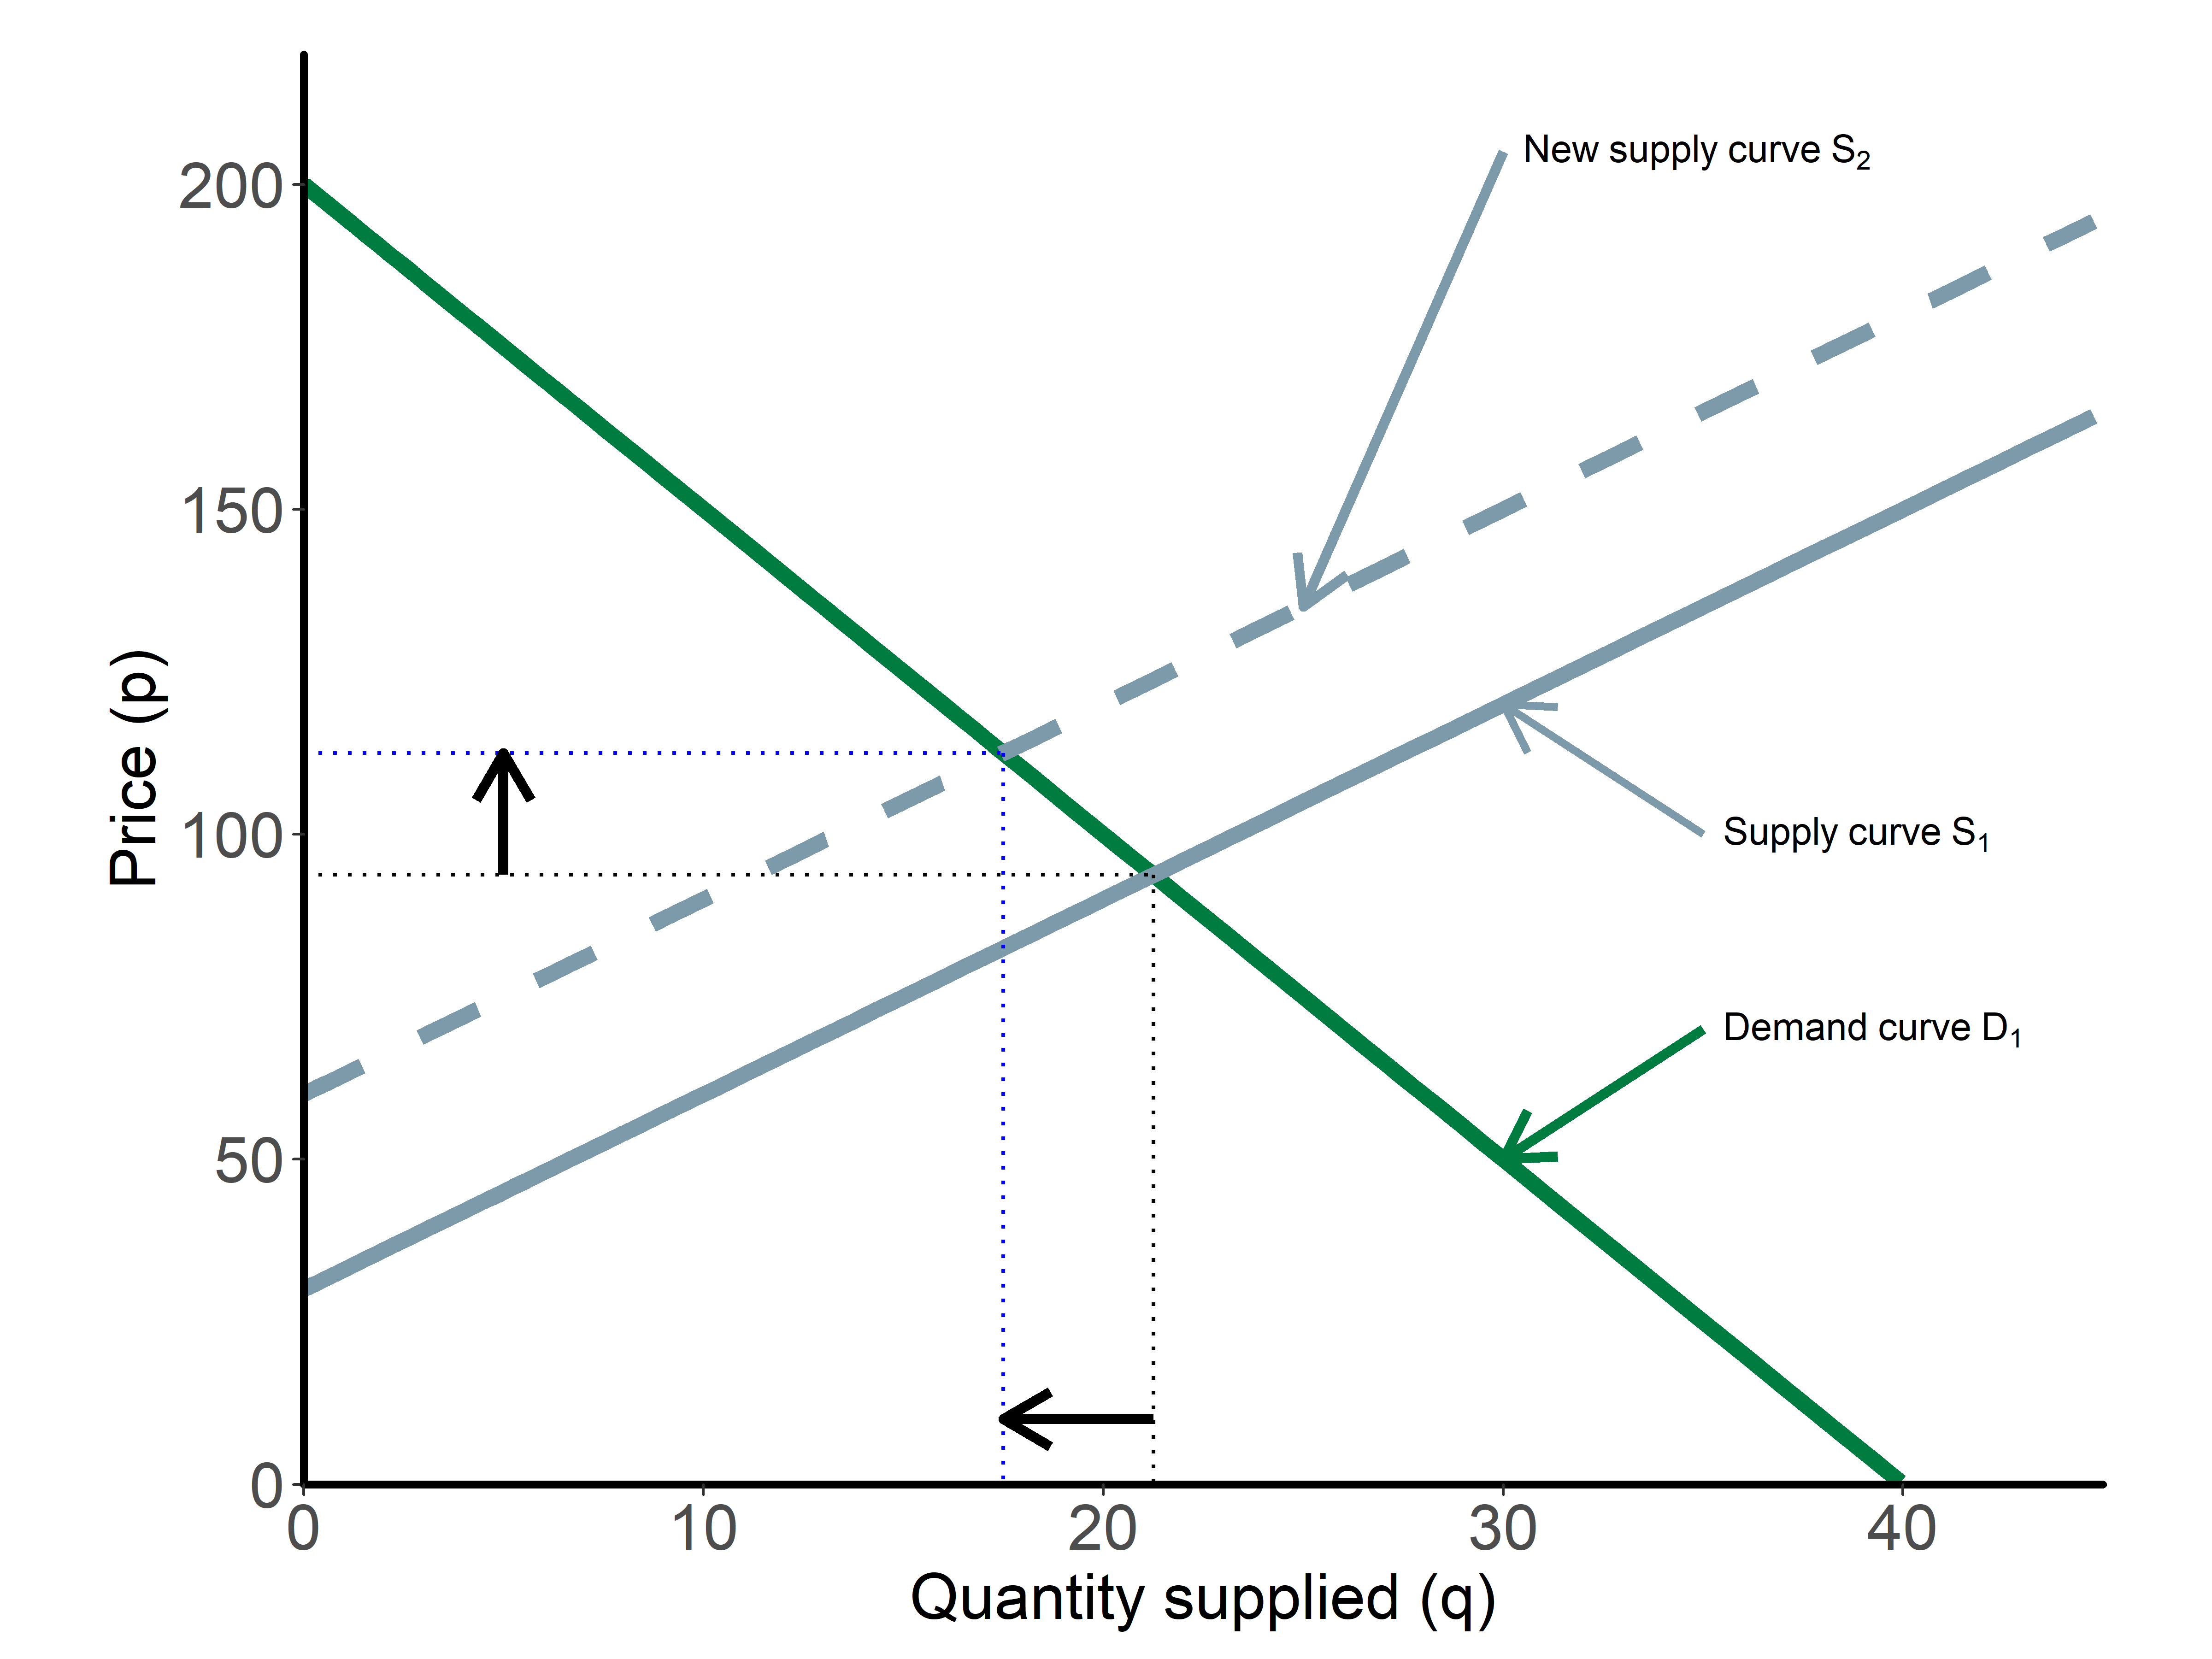
\includegraphics[width=\textwidth]{../images/equil_shift_crude.png}
}

\caption{The effects of an increase in the price of an input (crude oil in this case)}
\end{figure}
}

\frame{
	\frametitle{Shifts in Equilibrium: Shifting Supply}
	%	The demand for gasoline:
	
	\begin{figure}[t!]
    \center
	\resizebox{!}{.4\linewidth}{
    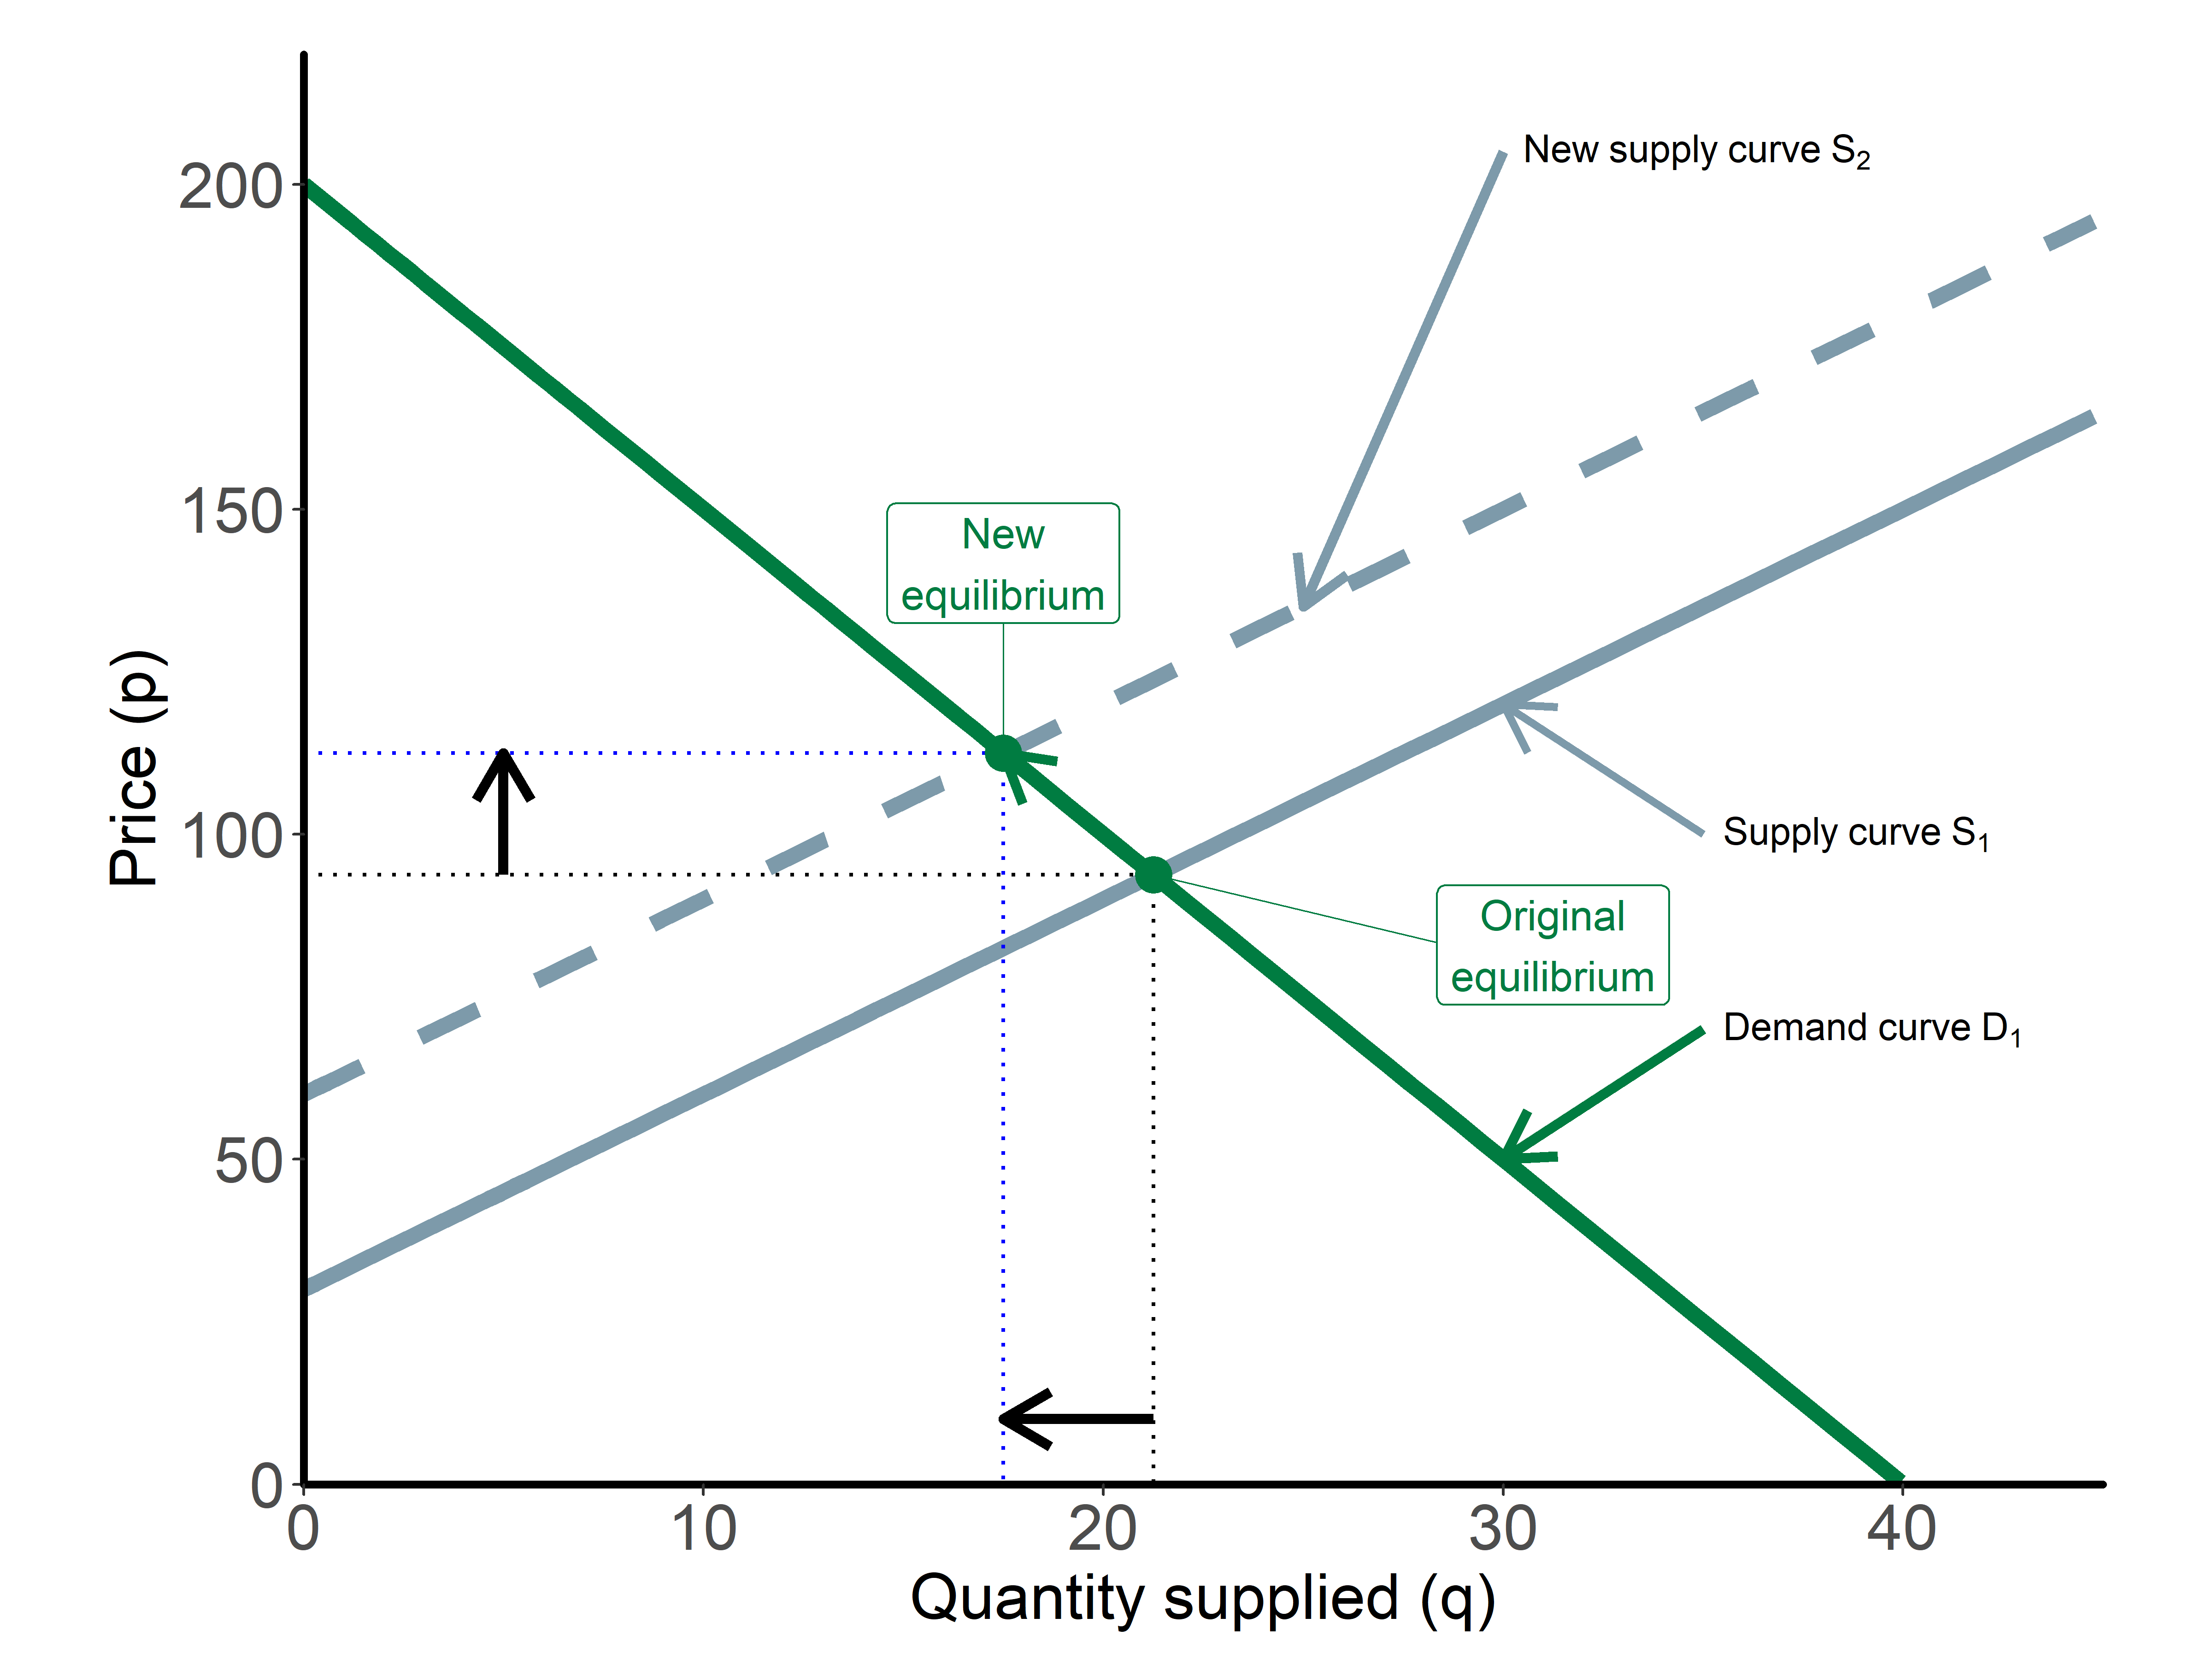
\includegraphics[width=\textwidth]{../images/equil_shift_mvmt.png}
}

\caption{The effects of an increase in the price of an input (crude oil in this case)}
\end{figure}
}




\frame{
	\frametitle{Shifts in Equilibrium: Shifting Supply}
		\begin{itemize}
	\item Recall that the original demand function was $Q_d = 40 - \frac{p}{5}$, with income of \$100,000, or $Y=100$. And the supply curve is $Q_s = 10 +   \frac{p}{3} - 0.5 p_{y}$. So, with crude at \$60 and income at \$100:
		\begin{align*}
		Q_{D} = 30 - \frac{p}{5} +.1(100) \quad \text{and} \quad Q_{S} = \frac{p}{3}-20
		\end{align*}
	\item In equilibrium $Q_{D}=Q_{S}$. Substituting yields:
		\begin{align*}
		40 - \frac{p}{5} &= \frac{p}{3}-20\\
		\frac{8p}{15} &=60 \, \rightarrow  p = 112.5
		\end{align*}
	\item Substituting $p = 112.5$ into $Q_{D}$ or $Q_{S}$ yields $Q=17.5$.
	\end{itemize}
}


\frame{
	\frametitle{Shifts in Equilibrium: Shifting Supply}
	\begin{itemize}
	\item And now we can compare the impacts of a shift in supply caused by a change in crude costs. In the initial equilibrium:
		\begin{align*}
		Q_{1}^* & = 21.25\\
		p_{1}^* & = 93.75
		\end{align*}
	\item In the \underline{new} equilibrium after the shift in income.
		\begin{align*}
		Q_{2}^* & = 17.5\\
		p_{2}^* & = 112.50
		\end{align*}
	\item The \underline{change} in the price of an input leads to a \underline{shift in supply}, and a \underline{movement along the demand curve} such that:
		\begin{align*}
		\Delta_p&=18.75\\
        \Delta_Q&=-3.75
		\end{align*}
	\end{itemize}
}




\frame{
	\frametitle{Shifts in Equilibrium: Shifting Supply}
	%	The demand for gasoline:
	
	\begin{figure}[t!]
    \center
	\resizebox{!}{.4\linewidth}{
    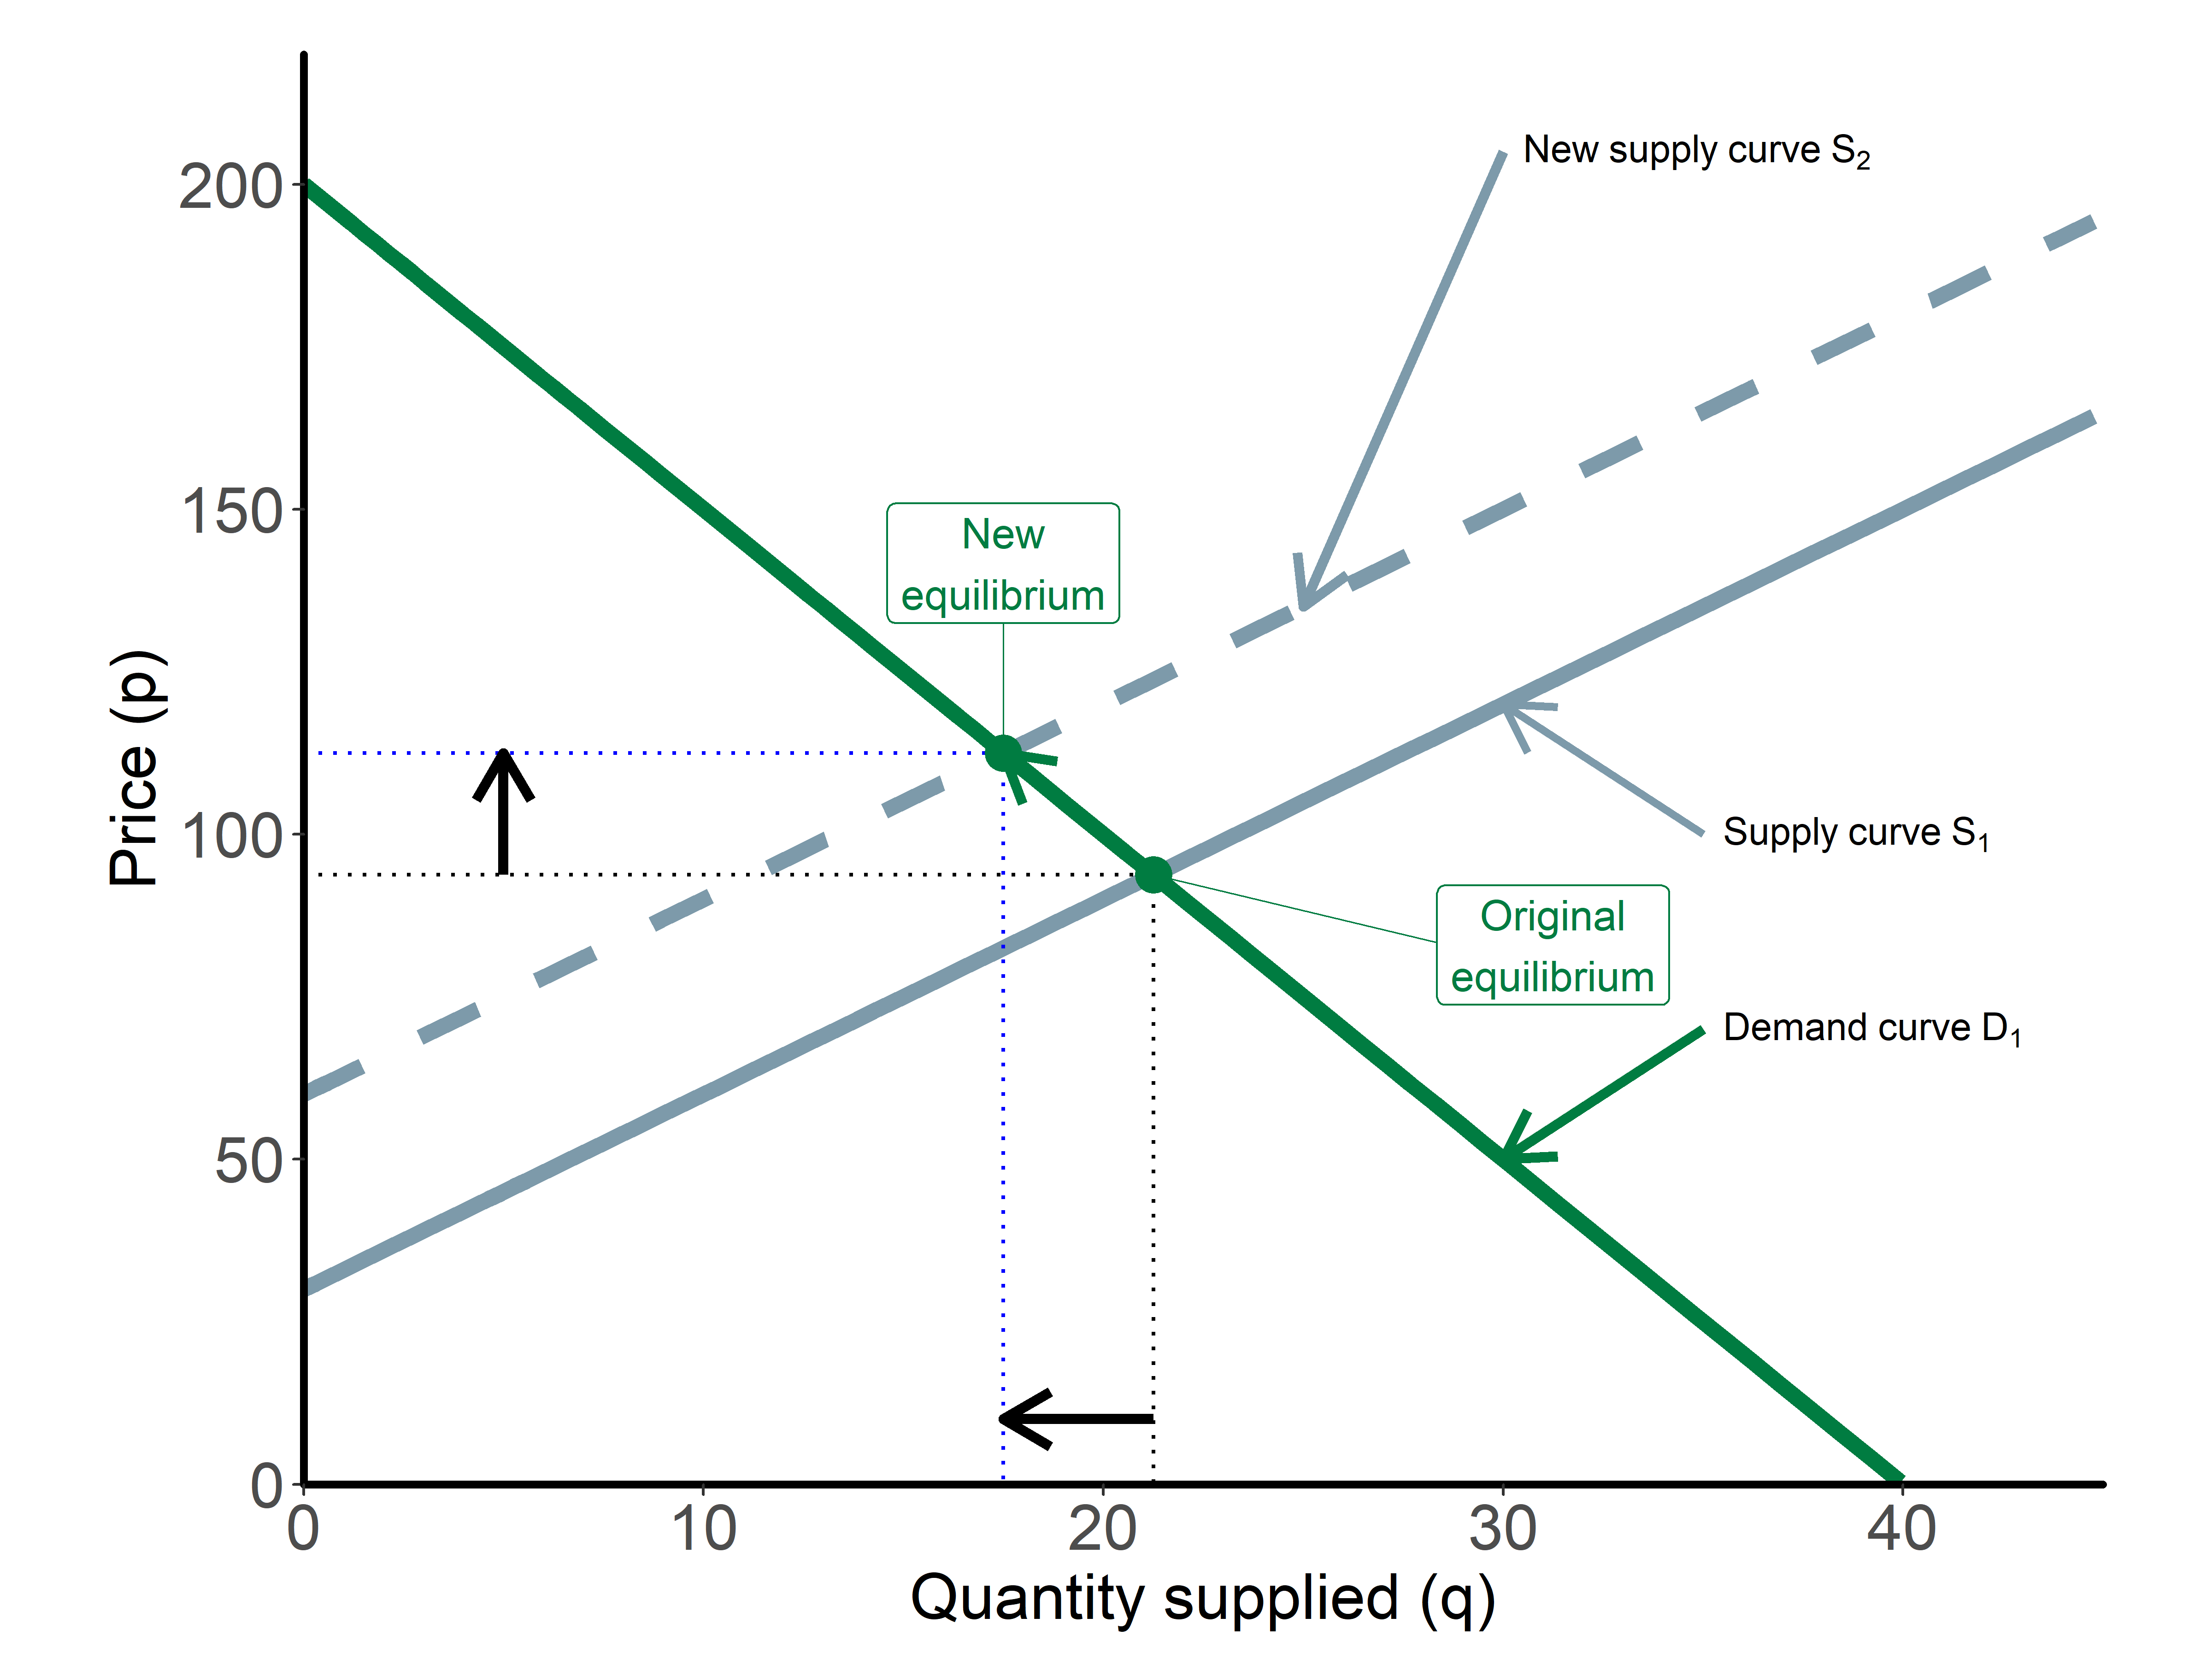
\includegraphics[width=\textwidth]{../images/equil_shift_mvmt.png}
}

\caption{The effects of an increase in the price of an input (crude oil in this case)}
\end{figure}
}




\frame{
	\frametitle{Shifts in Equilibrium: Concurrent Shifts}
	\begin{itemize}
	\item Sometimes, demand and supply change at the same time.
	\item[]
	\item Think of Alberta where increases in the oil price generally have substantial positive income effects (i.e. an increase in the oil price leads to an increase in household income, and vice versa).
	\item[]
	\item What would the effects of the combination of the two shifts we've just seen be on the equilibrium price and quantity in the market for gasoline?
	\end{itemize}
}

\frame{
	\frametitle{Shifts in Equilibrium: Concurrent Shifts in Demand and Supply}
	%	The demand for gasoline:
	
	\begin{figure}[t!]
    \center
	\resizebox{!}{.4\linewidth}{
    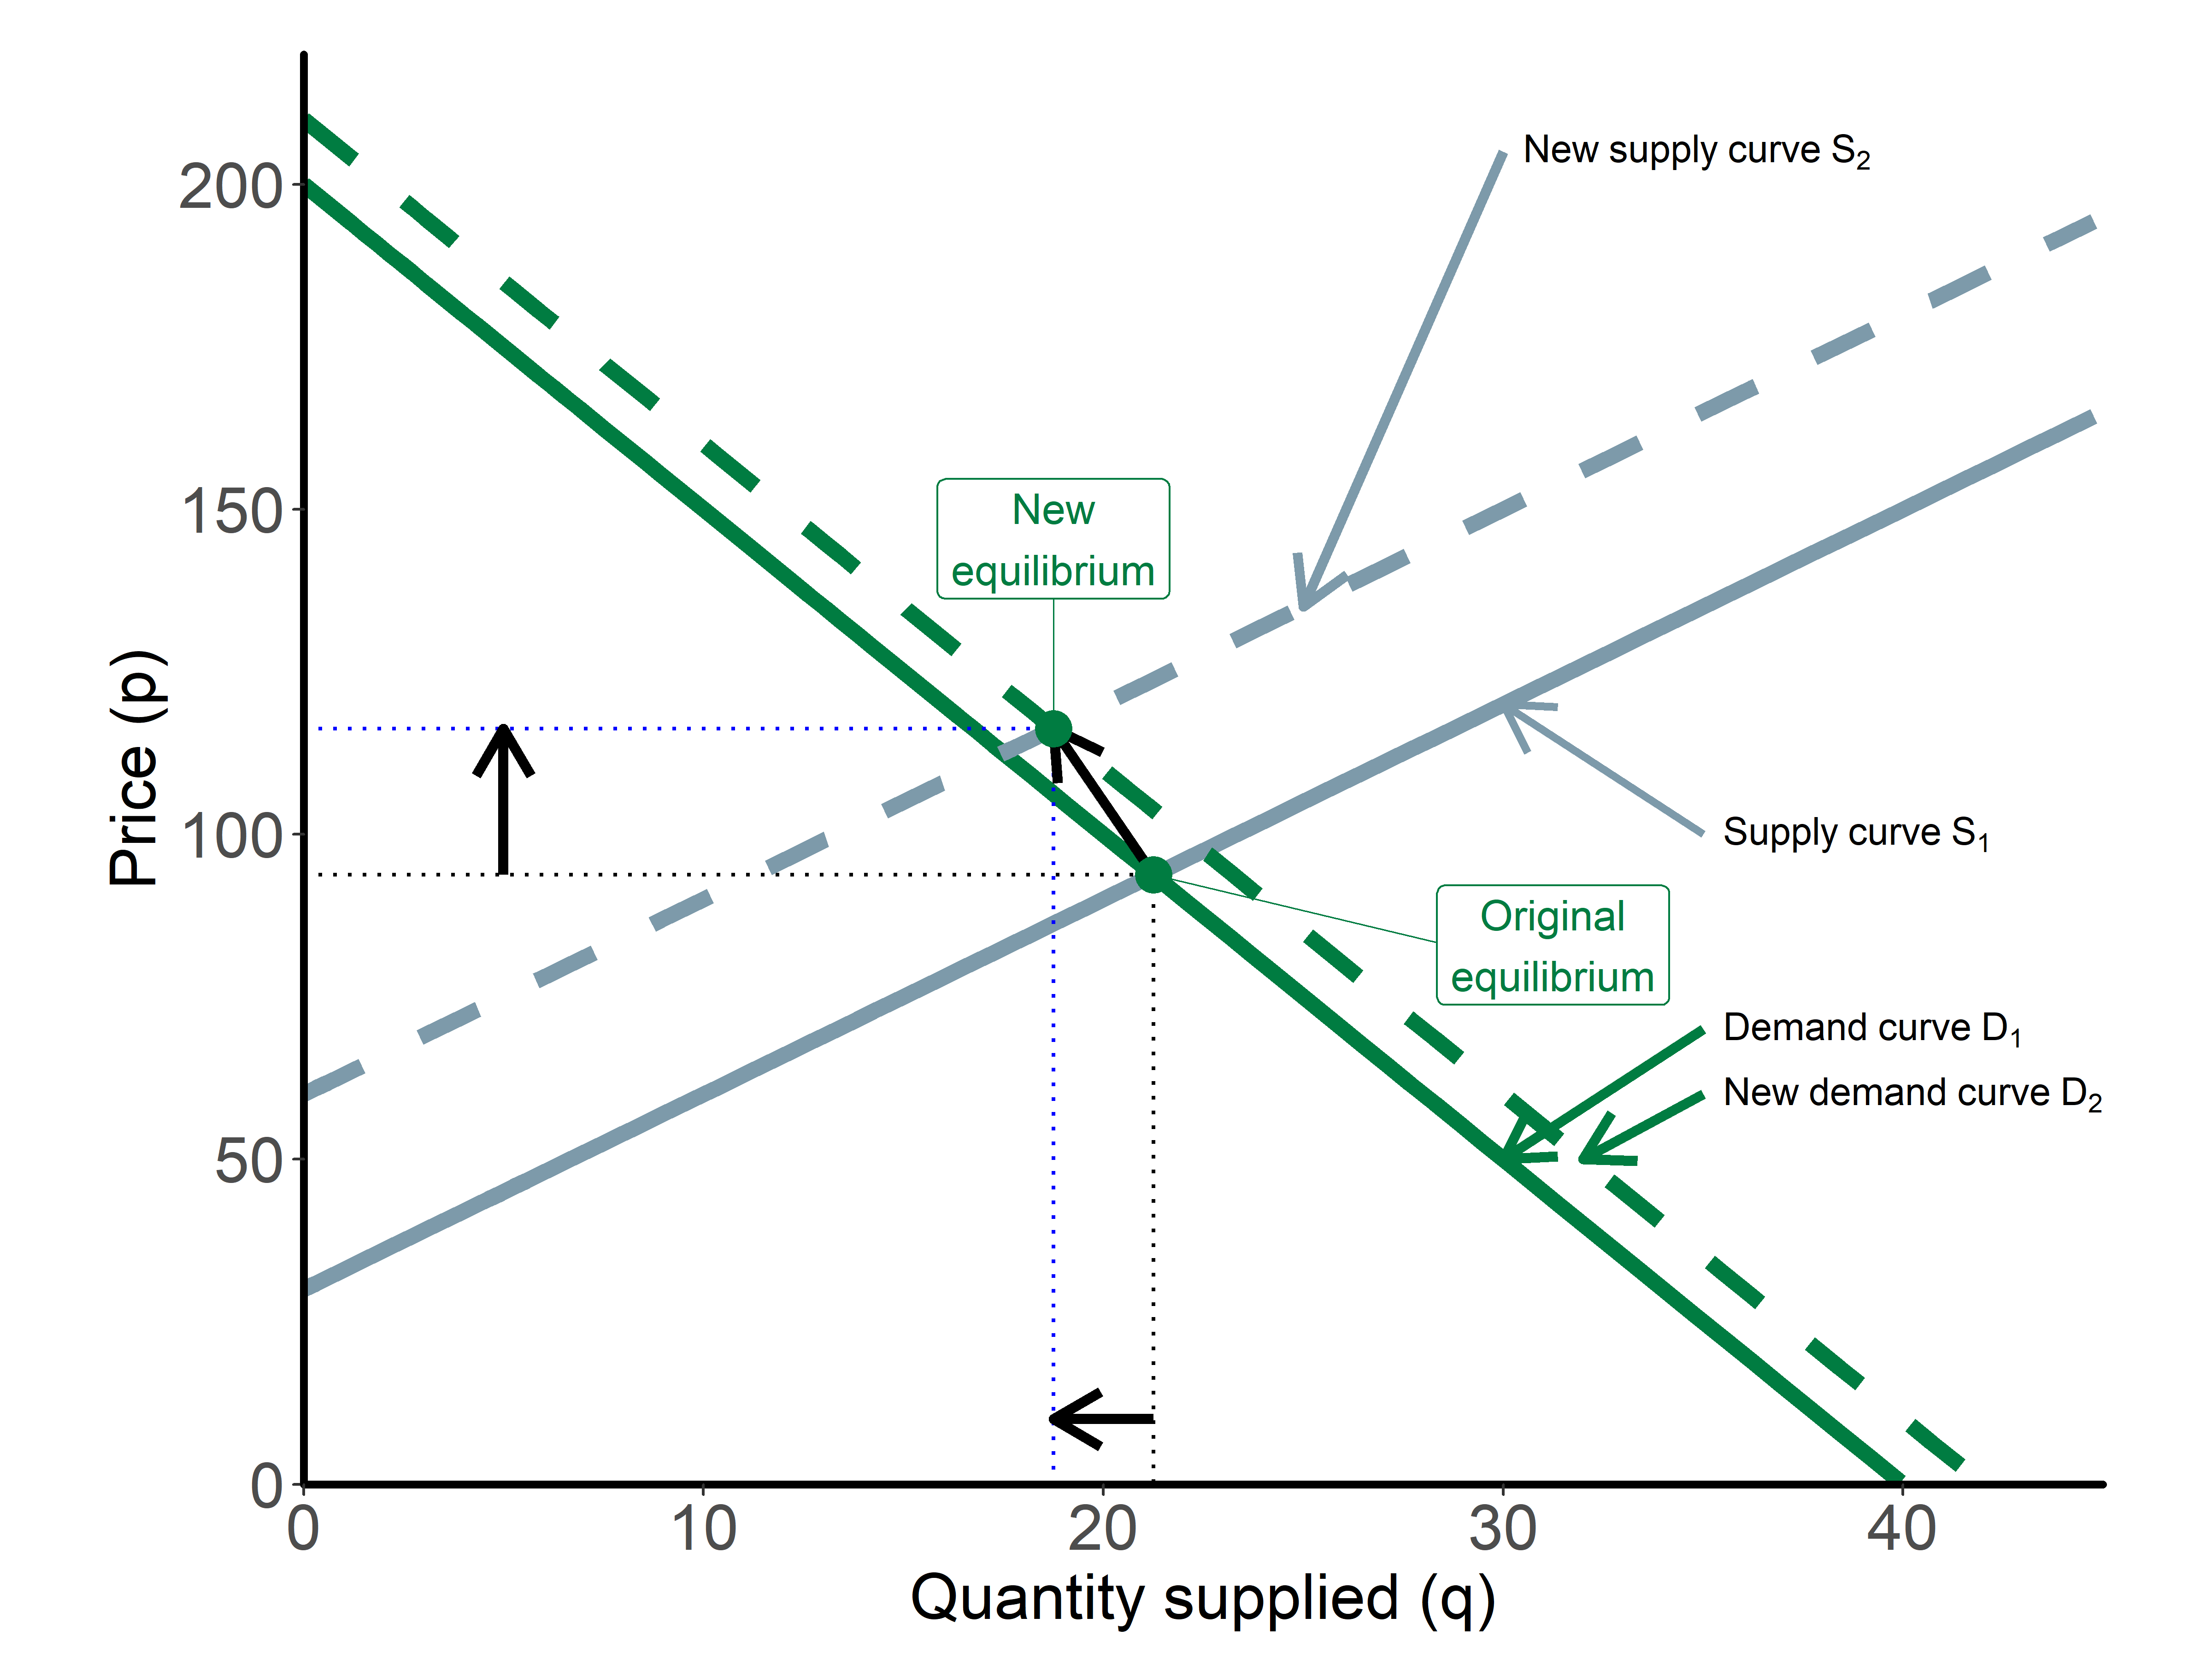
\includegraphics[width=\textwidth]{../images/equil_shift_both.png}
}

\caption{Income (demand) and input cost (supply) effects of an increase in the price of crude oil}
\end{figure}
}

\frame{
	\frametitle{Shifts in Equilibrium: Concurrent Shifts}
	\begin{itemize}
	\item When demand and supply change at the same time, we may not be able to sign the effects on prices and quantities without further analysis:
	\begin{itemize}
	\item An increase in demand (right shift) and a decrease in supply (left shift) could lead to any combination of increases or decreases in $p$ and $Q$;
	\item If demand and supply both increase, we know that equilibrium quantities will increase, but the effect on price is ambiguous;
	\item If supply decreases and demand increases, we know that price will increase, but the effect on quantities is ambiguous.
	\end{itemize}
\end{itemize}
}


\frame{
	\frametitle{Shifts in Equilibrium: Concurrent Shifts}
	\begin{itemize}
	\item When demand and supply change at the same time, the sizes of the shifts and the price elasticities of demand and supply determine the outcome.
\item Recall that the price elasticity of demand is the percentage change in quantity demanded for a given percentage change in price;
\begin{align*}
  \epsilon=\frac{\text{percentage change in quantity demanded}}{\text{percentage change in price}}=\frac{\Delta Q/Q}{\Delta p/p}=\frac{\Delta Q}{\Delta p}\frac{p}{Q}
\end{align*}
	\item The elasticity of supply is calculated similarly as the percentage change in quantity supplied for a given percentage change in price;
  	\item Hint: more \textit{elastic} is more responsive:
\small{\begin{itemize}\item \textit{inelastic} demand or supply means an elasticity less than one (i.e. the relative magnitude of the quantity response is smaller than the price change)
\item \textit{perfectly inelastic} demand has an elasticity of zero
\item \textit{perfectly elastic} demand has undefined elasticity
\end{itemize}}
\end{itemize}
}


\frame{
	\frametitle{Shifts in Equilibrium: Government Intervention}
	\begin{itemize}
	\item Government actions can also affect market outcomes.
	\item[]
	\item Three key channels:
		\begin{enumerate}
		\item Curve shifts.
		\item Price controls.
		\item Taxes/Subsidies.
		\end{enumerate}
	\end{itemize}
}

\frame{
	\frametitle{Shifts in Equilibrium: Policies that Shift Curves}
	\begin{itemize}
	\item Governments use three main approaches to shift curves:
		\begin{enumerate}
		\item Limits on who can buy.
			\begin{itemize}
			\item Governments can restrict who can buy certain products (e.g. cigarettes to
children). This shifts the demand curves for these products
to the left by shrinking the market, and thus decreases the quantity demanded at any price.
			\end{itemize}
		\item Restrictions on imports or exports.
			\begin{itemize}
			\item Governments can restrict the flow of imports or exports. Import restrictions artificially shifts the importing country's supply curve to the left, while restrictions on exports shift the exporting country's demand curve to the left.
			\end{itemize}
		\item Government purchases.
			\begin{itemize}
			\item Governments can buy goods directly, increasing the quantity demanded at each
price. This shifts the demand curve to the right.
			\end{itemize}
		\end{enumerate}
	\item Why would governments enact these policies?
	\end{itemize}
}

\frame{
	\frametitle{Shifts in Equilibrium: Price Controls}
	\begin{itemize}
	\item Sometimes governments intervene by controlling prices in a market.
	\item[]
	\item Two main forms:
		\begin{enumerate}
		\item \underline{Price ceiling}.
			\begin{itemize}
			\item Policy in which a government sets a maximum price, $\bar{p}$, that can prevail
in the market.
			\end{itemize}
		\item \underline{Price floor}.
			\begin{itemize}
			\item Policy in which a government sets a minimum price, $\underline{p}$, that can
prevail in the market.
			\end{itemize}
		\end{enumerate}
	\end{itemize}
}

\frame{
	\frametitle{Shifts in Equilibrium: Price Controls}
	%	The demand for gasoline:
	\begin{figure}[t!]
    \center
	\resizebox{!}{.4\linewidth}{
    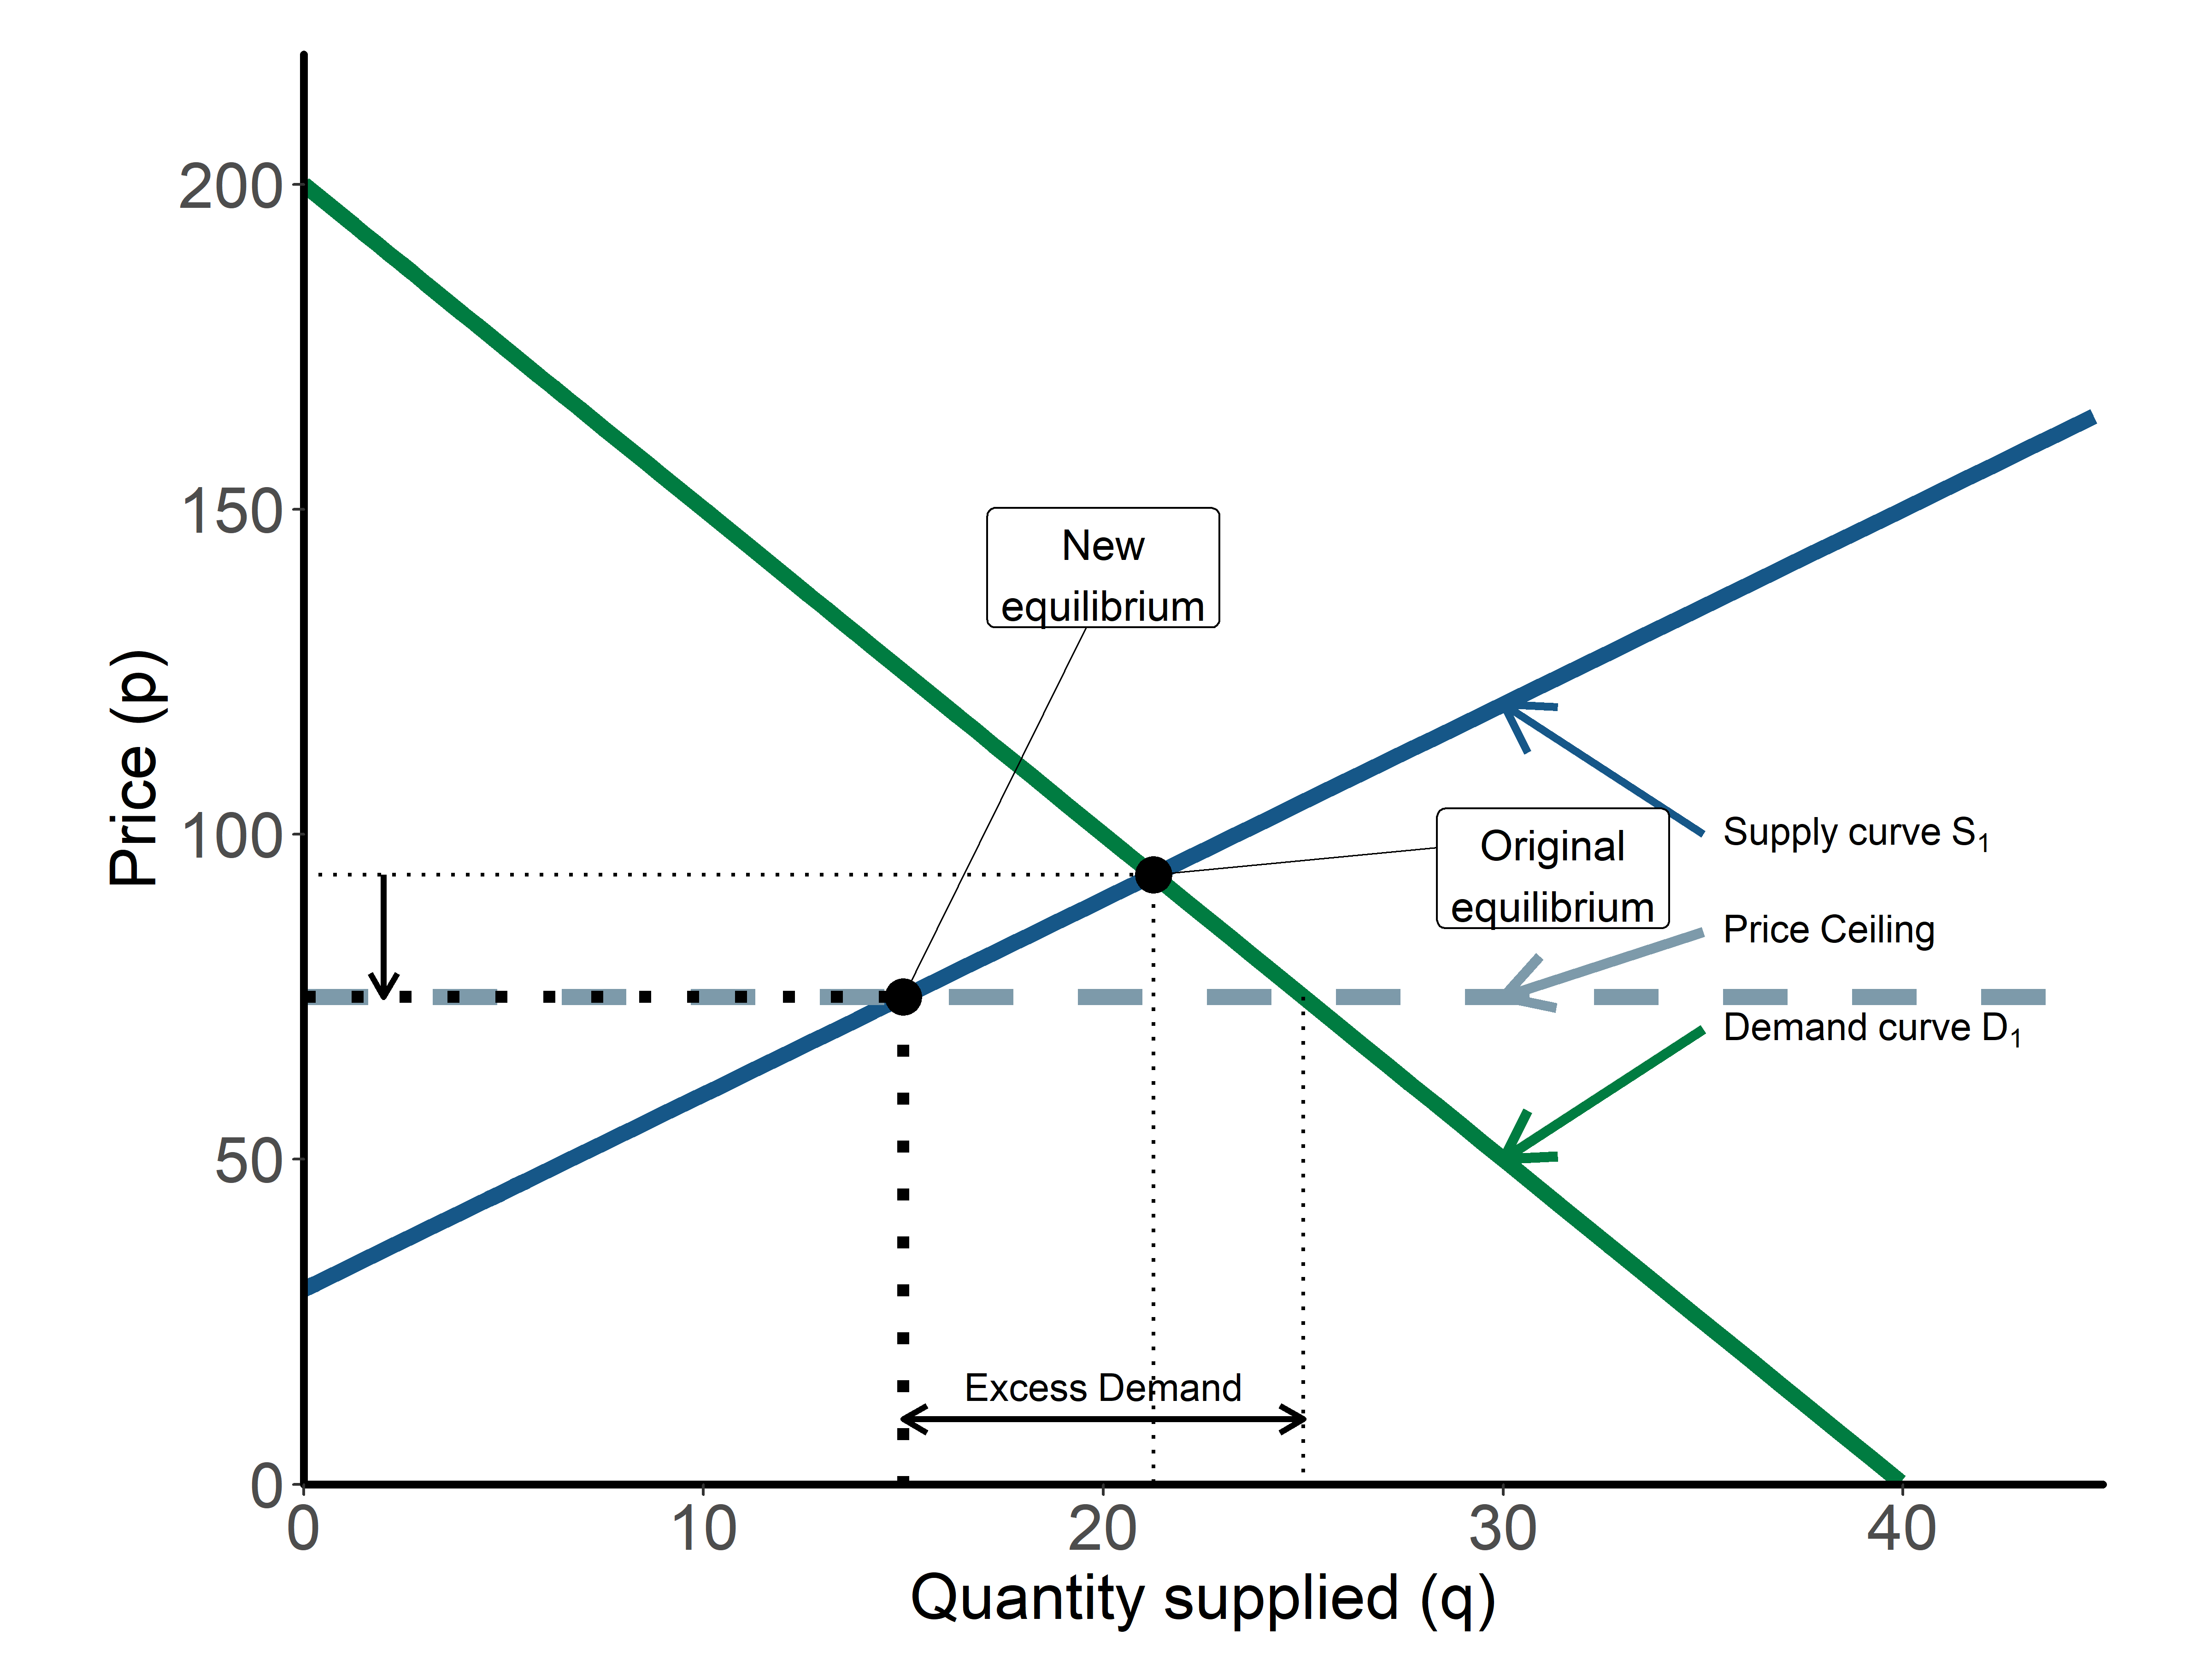
\includegraphics[width=\textwidth]{../images/equil_price_ceiling.png}
}
\caption{The effects of a maximum price in the market.}
\end{figure}
}

\frame{
	\frametitle{Shifts in Equilibrium: Price Controls}
	%	The demand for gasoline:
	\begin{figure}[t!]
    \center
	\resizebox{!}{.4\linewidth}{
    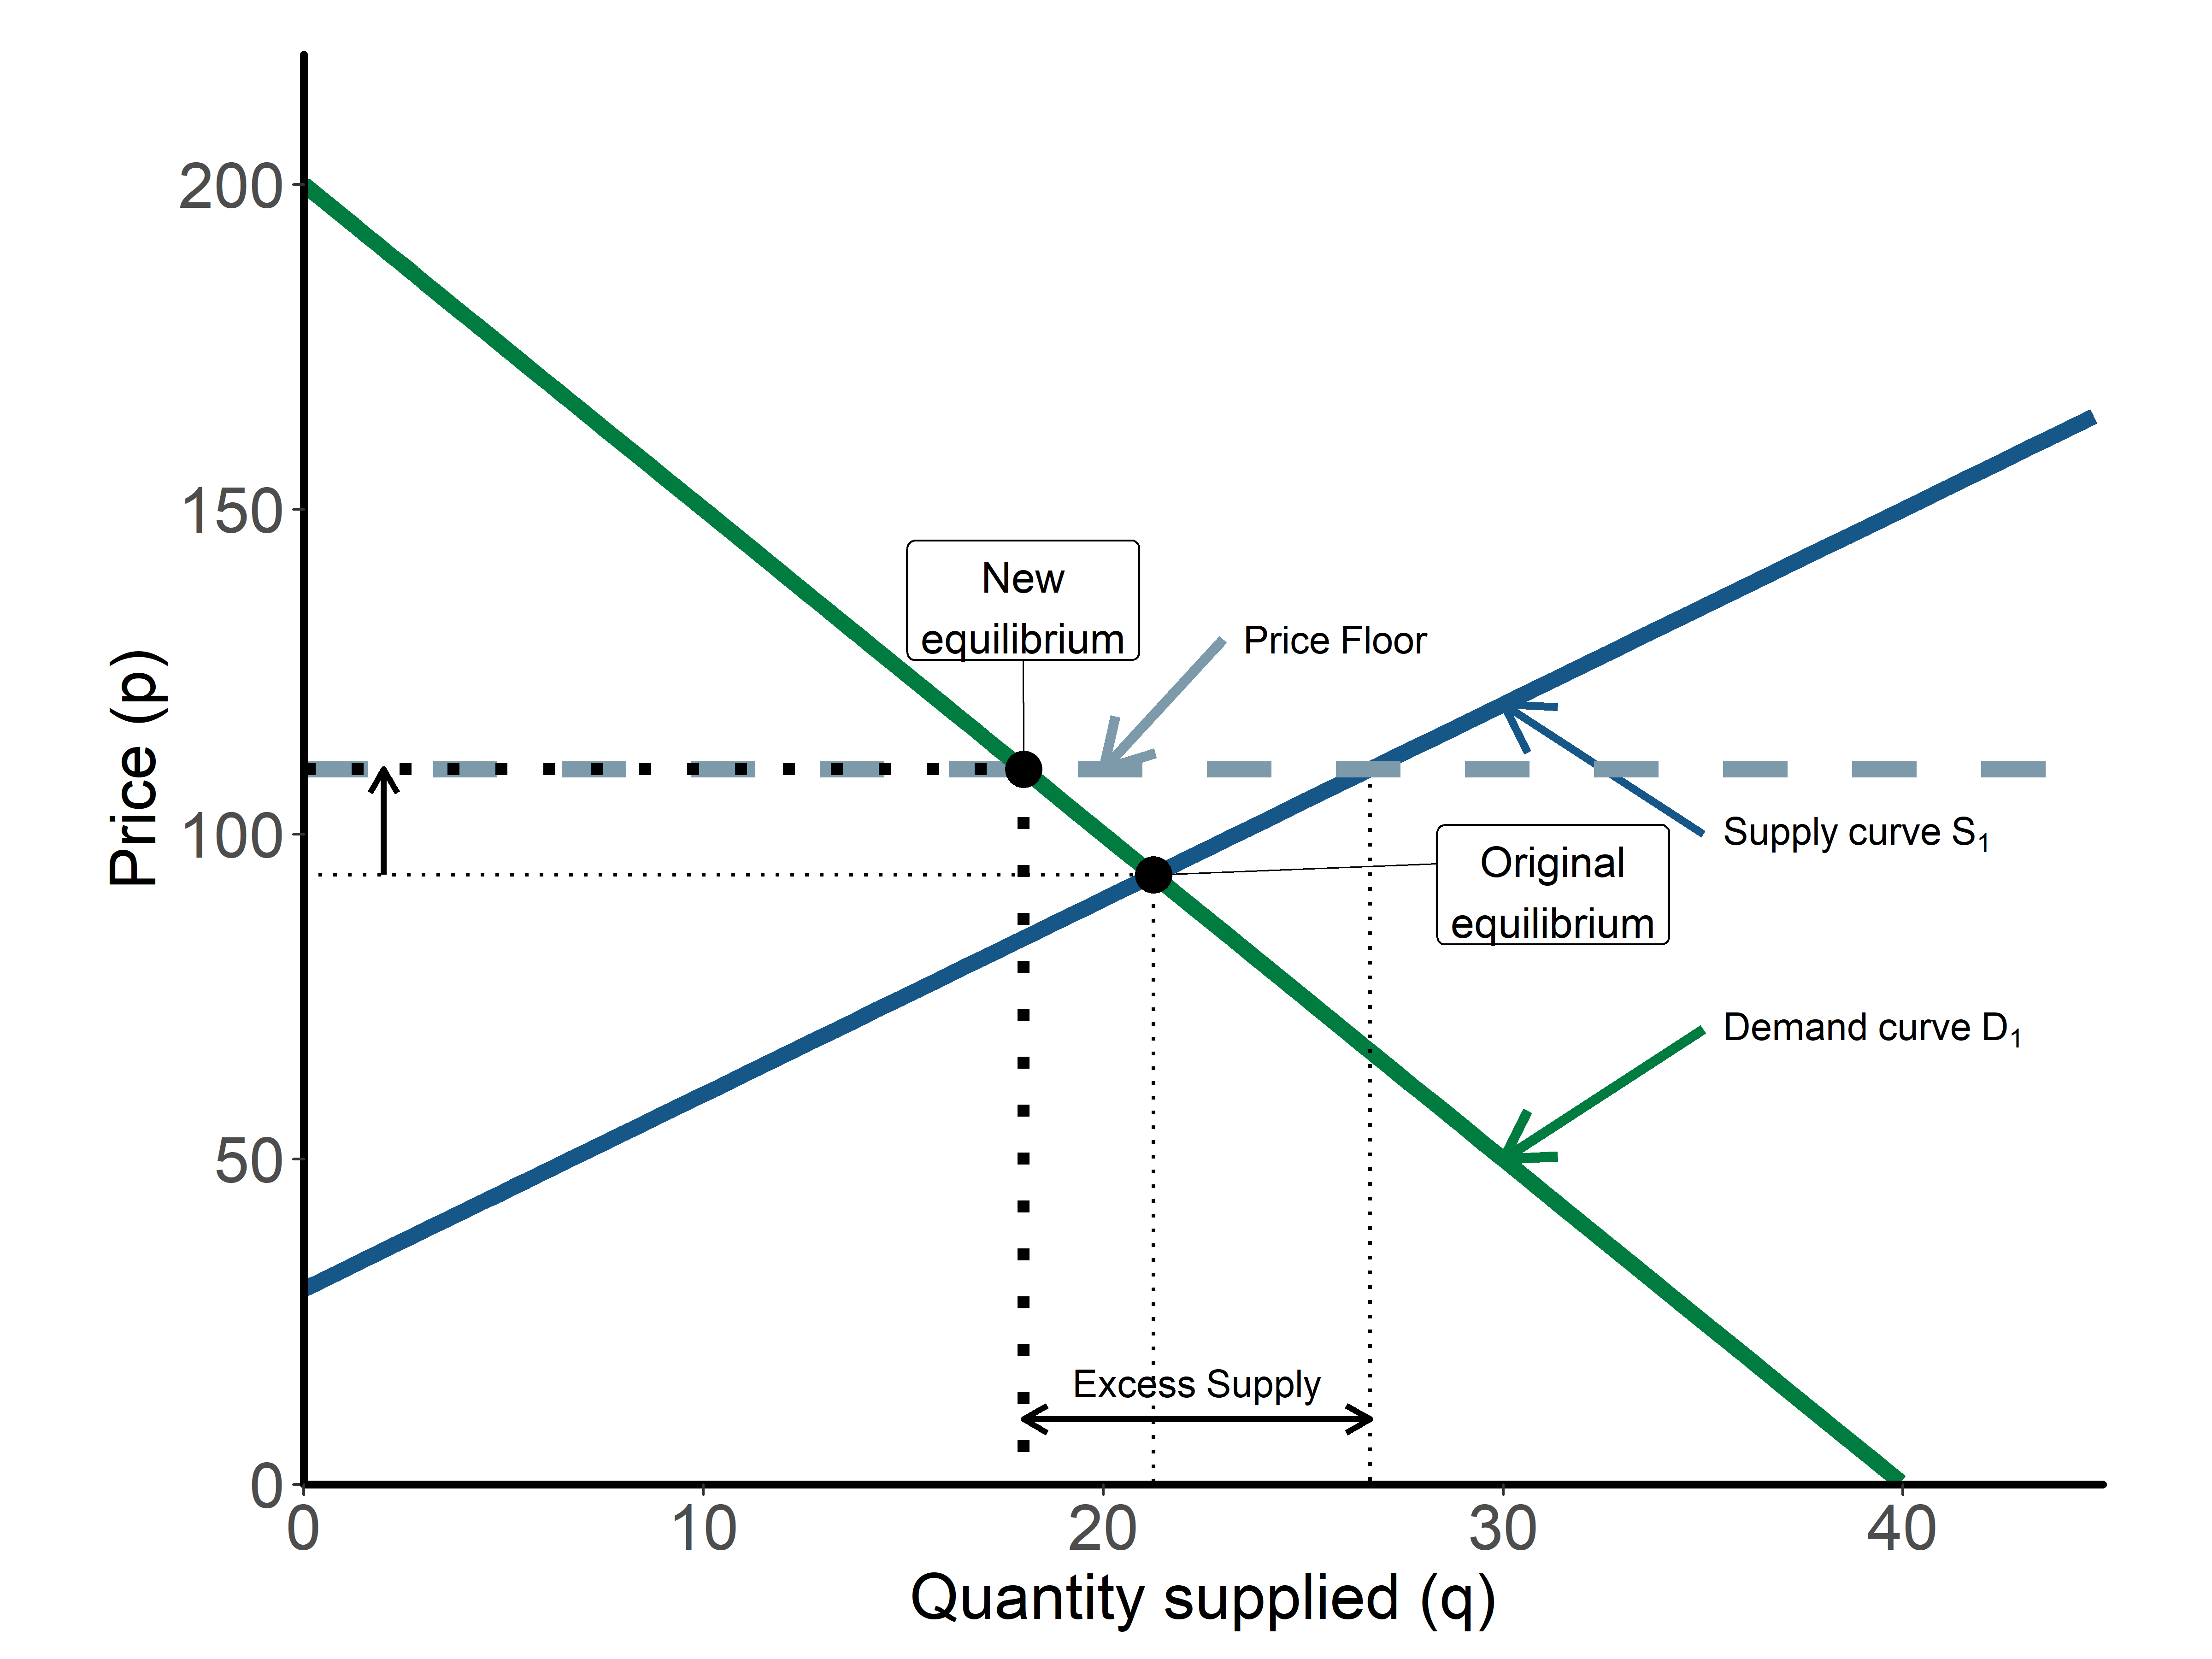
\includegraphics[width=\textwidth]{../images/equil_price_floor.png}
}
\caption{The effects of a minimum price in the market.}
\end{figure}
}


\frame{
	\frametitle{Shifts in Equilibrium: Price Controls}
	\begin{itemize}
	\item Examples show that supply need not equal demand if the government intervenes in the market.
	\item[]
	\item In the absence of government intervention, supply equals demand, and the market clears.
	\item[]
	\item With government intervention, the quantity demanded and quantity supplied need not equal
the \underline{actual} quantity that is bought and sold.
	\end{itemize}
}

\frame{
	\frametitle{Shifts in Equilibrium: Taxes/Subsidies}
	\begin{itemize}
	\item Taxes may also affect equilibrium price and quantity.
	\item[]
	\item As an example, we will examine the effects of a \textit{specific tax} in the market for
gasoline.
		\begin{itemize}
		\item A specific tax is a tax charged per unit of output (e.g. \$/litre of gasoline).
		\end{itemize}
	\end{itemize}
}

\frame{
	\frametitle{Shifts in Equilibrium: Specific Tax Collected from Suppliers}
	%	The demand for gasoline:
\begin{figure}[t!]
    \center
	\resizebox{!}{.4\linewidth}{
    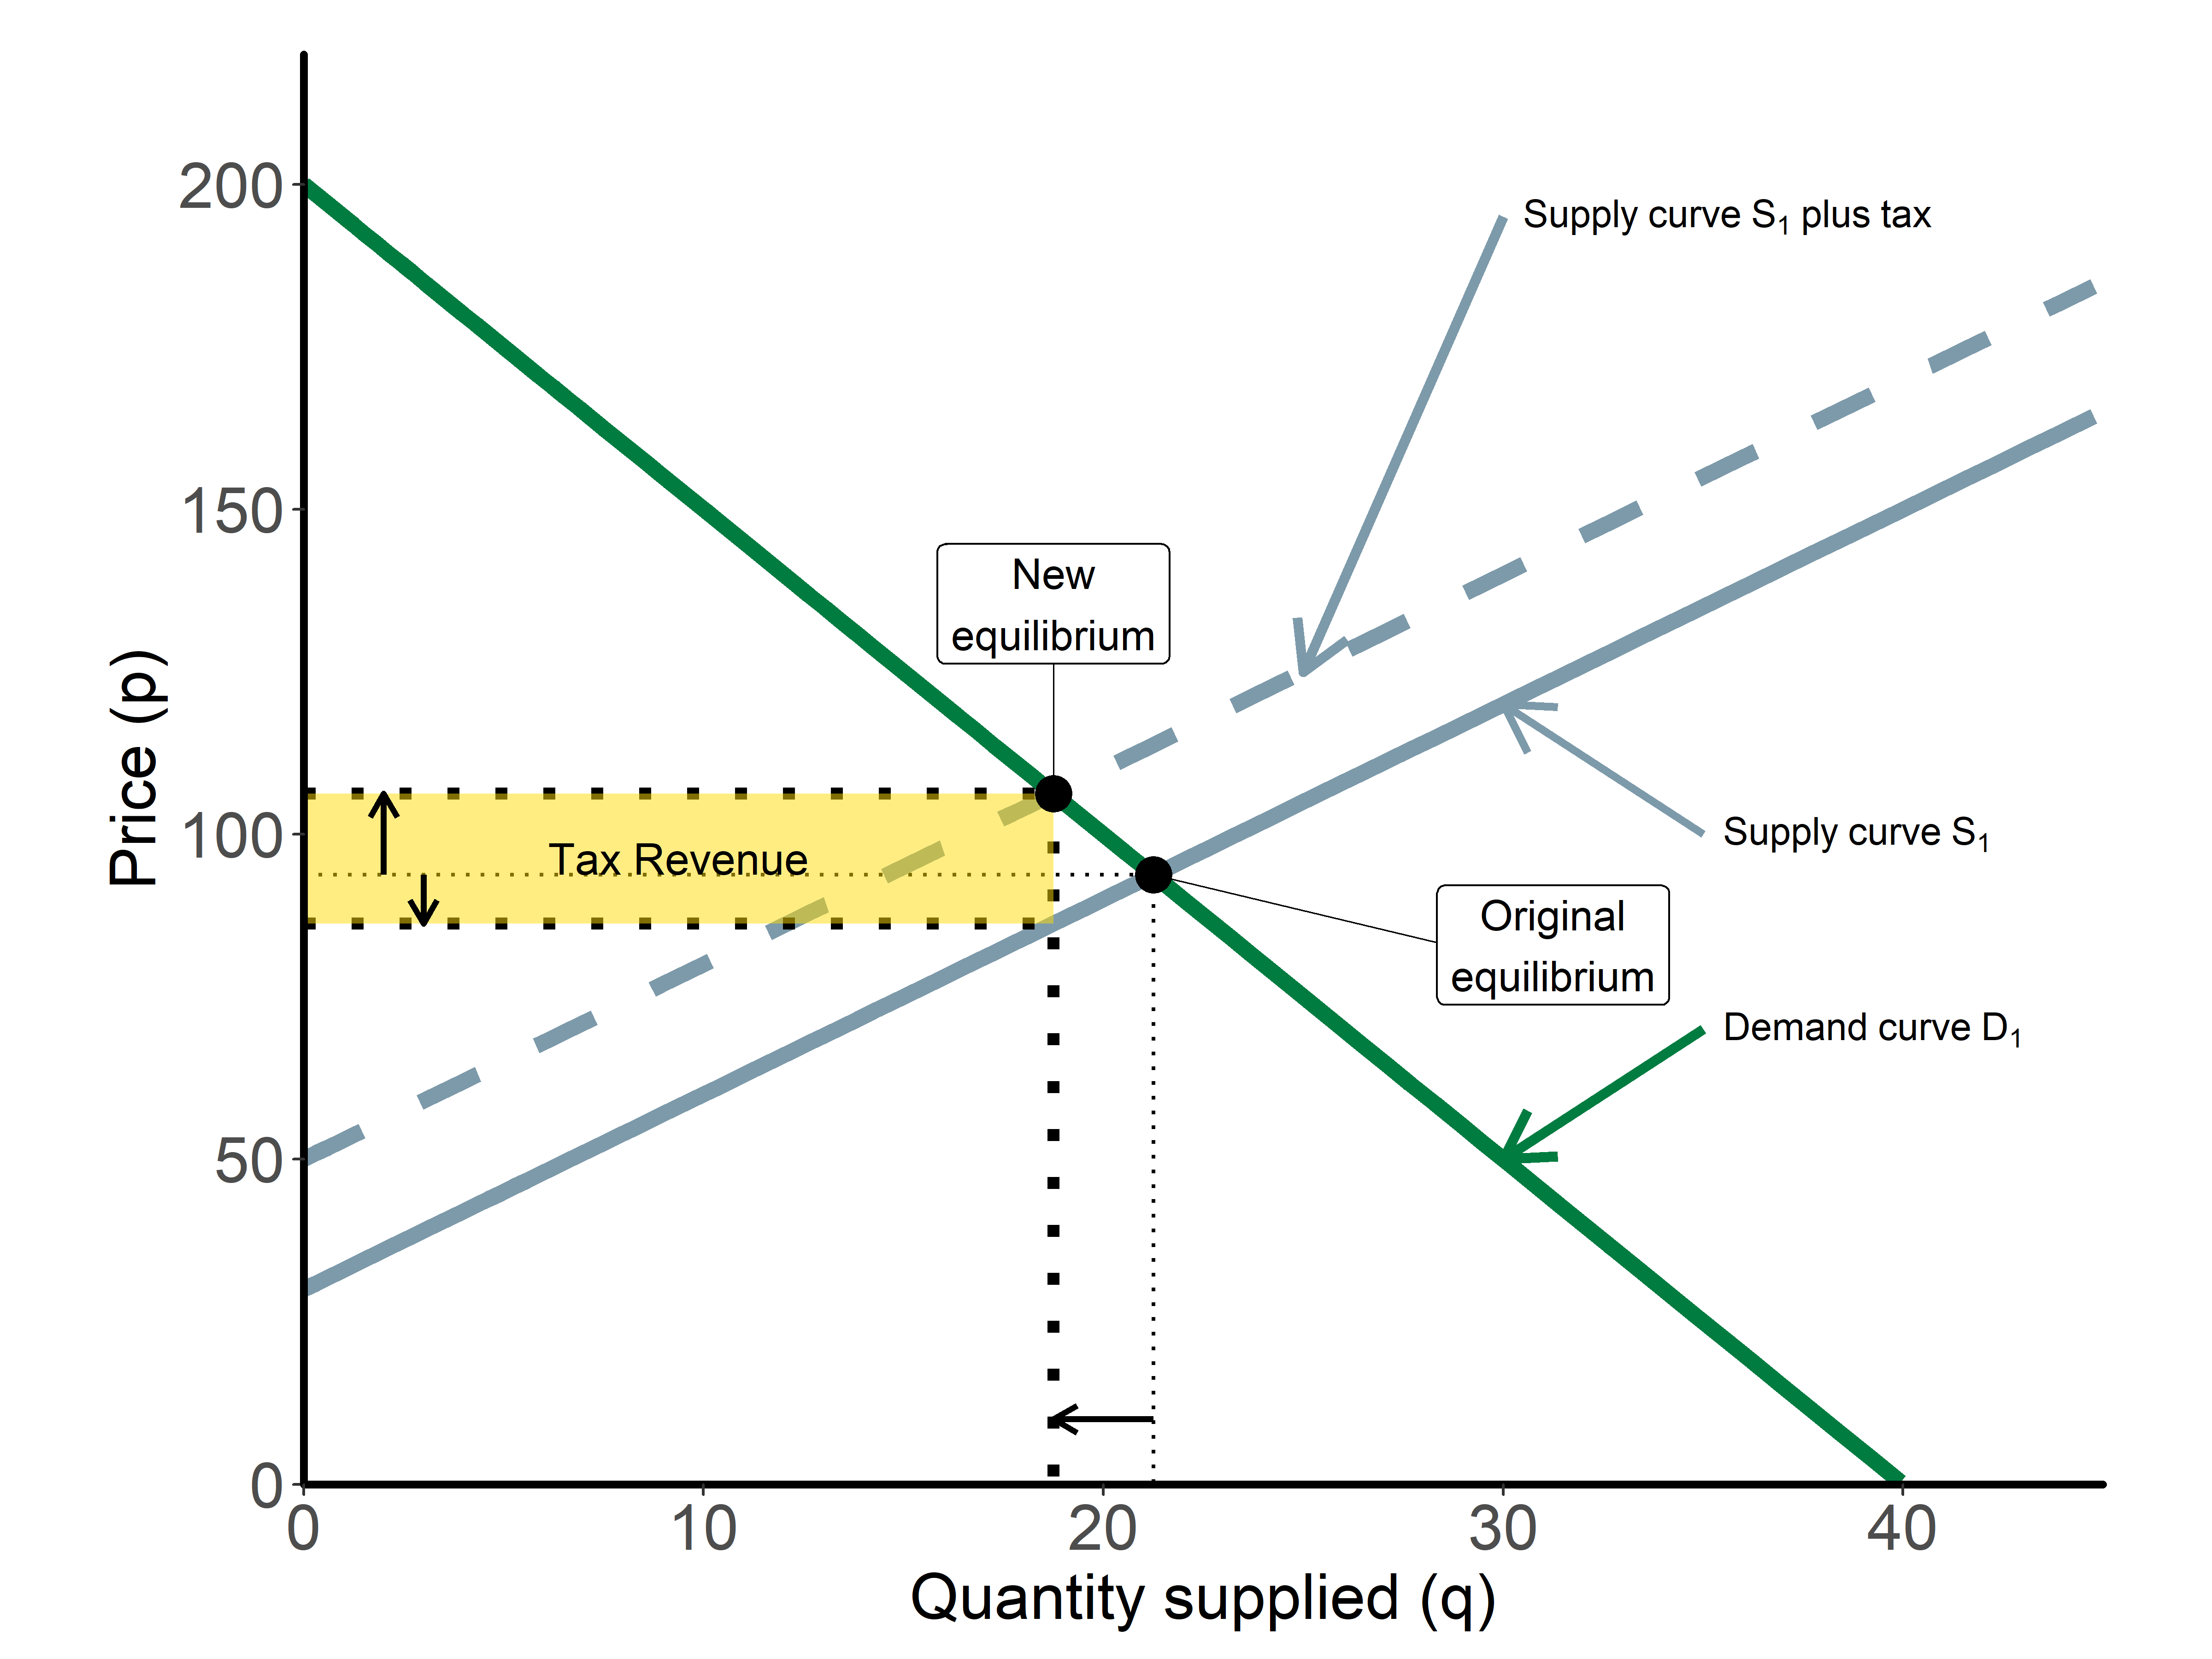
\includegraphics[width=\textwidth]{../images/equil_shift_tax_supply.png}
}
\caption{The effects of a 20c/l tax charged to gasoline producers}
\end{figure}
}

\frame{
	\frametitle{Shifts in Equilibrium: Specific Tax Collected from Consumers}
	%	The demand for gasoline:
\begin{figure}[t!]
    \center
	\resizebox{!}{.4\linewidth}{
    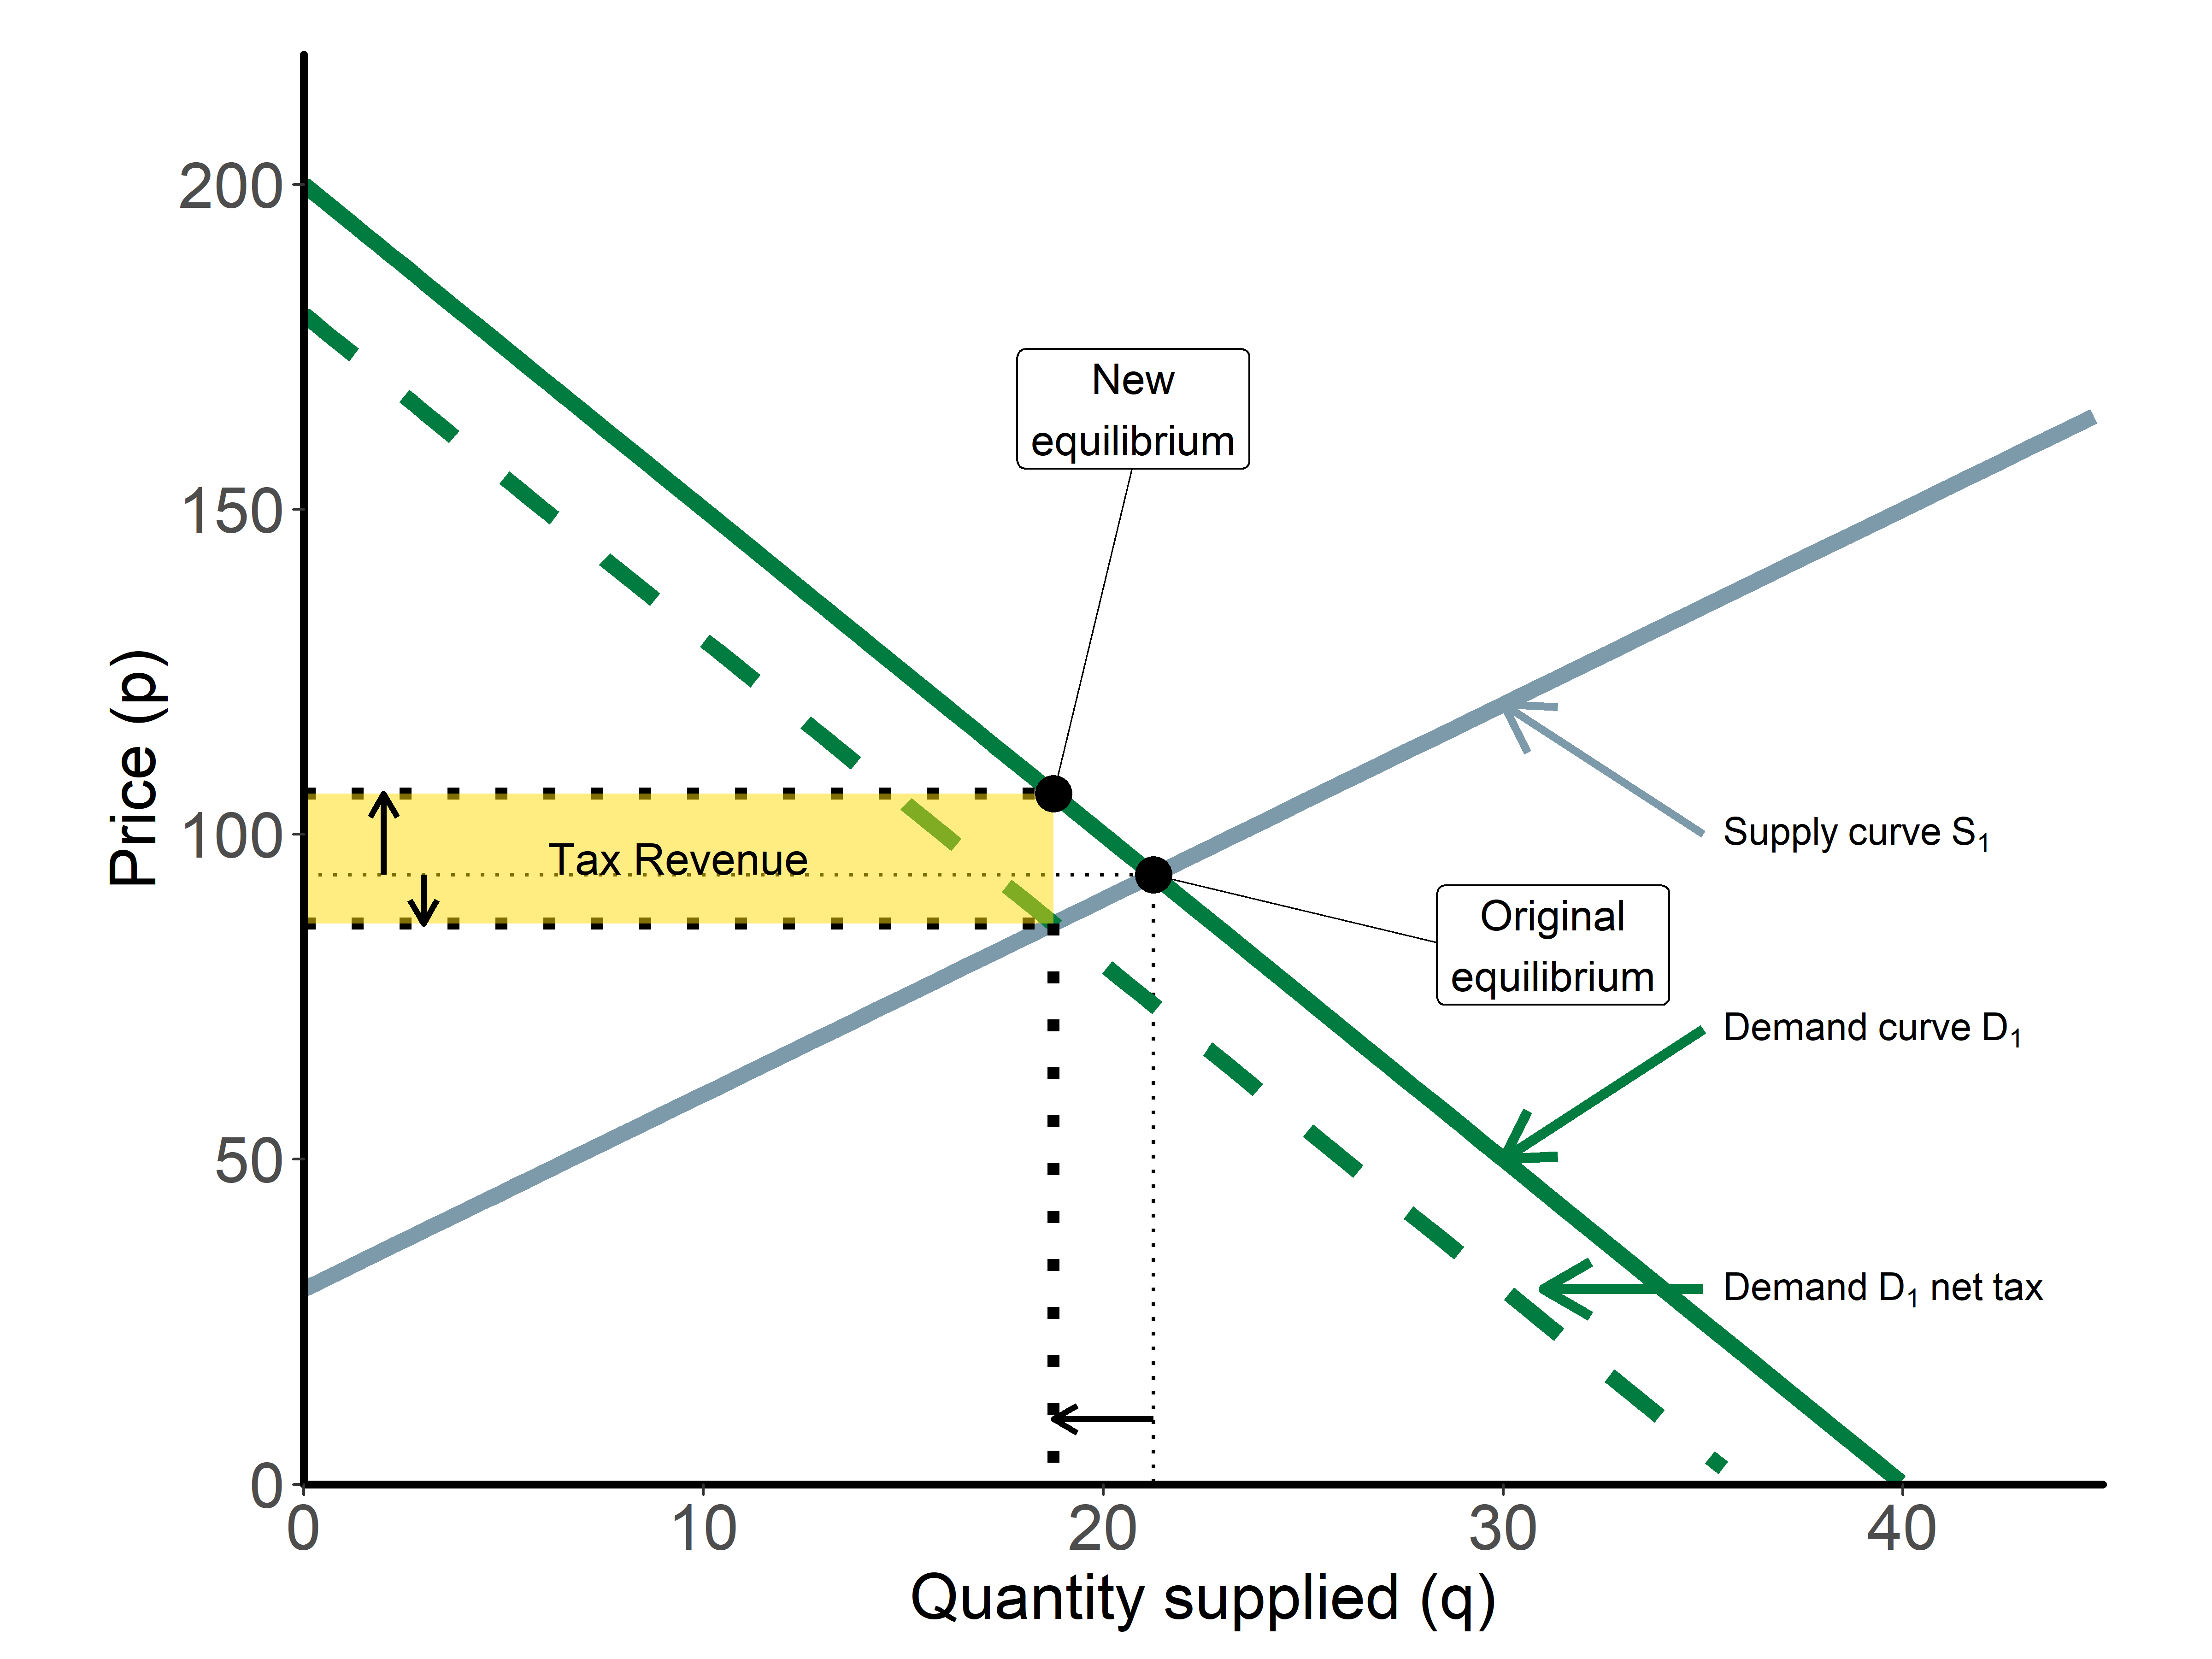
\includegraphics[width=\textwidth]{../images/equil_shift_tax_demand.png}
}
\caption{The effects of a 20c/l tax charged to gasoline consumers}
\end{figure}
}


\frame{
	\frametitle{Shifts in Equilibrium: The Effects of A Specific Tax}
	\begin{itemize}
	\item Two key points:
		\begin{enumerate}
		\item As shown in the two figures, the imposition of specific sales tax yields the same
equilibrium regardless of \textit{who pays the tax}.
		\item[]
		\item The figures also show that the tax need not be fully passed on to consumers.
			\begin{itemize}
			\item Producers may bear some of the effects of a tax.
			\item What determines the extent of pass-through?
			\end{itemize}
		\end{enumerate}
	\end{itemize}
}

\frame{
	\frametitle{Outline}
	\begin{enumerate}
%	\item Big Government Gasoline
%	\item[]
	\item The Supply-and-Demand Model
		\begin{itemize}
		\item Demand
		\item Supply
		\item Market Equilibrium
		\end{itemize}
	\item[]
	\item Using the Model
		\begin{itemize}
		\item Changing fundamentals.
		\item The effects of government intervention.
		\end{itemize}
	\item[]
	\item \alert{Applying the model in practice.}
		\begin{itemize}
		\item When it works.
		\item When if fails.
		\end{itemize}
	\end{enumerate}
}

\section{Supply and Demand in Practice}

\frame{
	\frametitle{3. Applying the Model in Practice}
	\begin{itemize}
	\item The supply-and-demand model is a simple, but powerful tool for understanding how markets
will change in the future in response to shocks and changes in government policy.
		\begin{itemize}
		\item e.g. Dr. Copper, Mars Corp.
		\end{itemize}
	\item[]
	\item Unleashing the power of the model requires a deep understanding of the factors that will
affect demand and supply.
		\begin{itemize}
		\item Need to understand determinants of demand and supply/possible government actions.
		\end{itemize}
	\item[]
	\item We also need to know when the model is appropriate to use.
	\end{itemize}
}

\frame{
	\frametitle{3. Applying the Model in Practice}
	\begin{itemize}
	\item The supply-and-demand model works well as a tool for understanding markets that are
\textit{perfectly competitive}.
	\item Five characteristics of a perfectly competitive market:	
		\begin{enumerate}
		\item Many small buyers and sellers.
		\item Consumers believe all firms produce identical products.
		\item All market participants have full information about price and product
characteristics.
		\item Transaction costs (expenses over and above the price) are negligible.
		\item Firms can easily enter and exit the market, so competition is high.
		\end{enumerate}
	\item The model does not work well in non-competitive markets where there are a few sellers that
are price setters.
		\begin{itemize}
		\item For these markets, we need a different model.
		\end{itemize}
	\end{itemize}
}

\frame{
	\frametitle{3. Applying the Model in Practice}
	\begin{itemize}
	\item In practice, no market necessarily meets all five criteria.
	\item[]
	\item Still, the model is useful if the market is ``competitive enough''.
	\item[]
	\item What are some markets for which the model would work well?
	\end{itemize}
}

\frame{
	\frametitle{Supply and Demand: Takeaways}
	\begin{enumerate}
	\item The supply-and-demand model is a simple and powerful tool for understanding many markets.
	\item Model relates the quantity consumers demand and the quantity producers supply to own prices
and other factors.
	\item Using the model requires understanding how factors other than own price may shift demand
and supply, and how government intervention may affect prices in the market.
	\item The model works well for understanding markets that are \textit{competitive enough}.
	\end{enumerate}
}

\end{document}
